\documentclass[11pt,a4paper]{article}

\usepackage[indonesian]{babel}
\usepackage{fontspec}
\setmainfont{PlusJakartaSans}[
  Path=fonts/,
  Extension=.ttf,
  UprightFont=*-Regular,
  ItalicFont=*-Italic,
  BoldFont=*-Bold,
  BoldItalicFont=*-BoldItalic
]
\newfontfamily\judulfont{PlusJakartaSans}[Path=fonts/, Extension=.ttf, UprightFont=*-ExtraBold]
\newfontfamily\tebalfont{PlusJakartaSans}[Path=fonts/, Extension=.ttf, UprightFont=*-SemiBold]

\usepackage[a4paper,top=2.5cm,bottom=2.6cm,left=2.5cm,right=2.5cm,headheight=15pt]{geometry}
\usepackage{xcolor}
\definecolor{tinta}{HTML}{1C2230}
\definecolor{biru}{HTML}{4A7FDB}
\definecolor{redup}{HTML}{5B6475}
\definecolor{garis}{HTML}{DDE3EE}
\definecolor{latar}{HTML}{EEF3FC}

\usepackage{graphicx}
\usepackage[export]{adjustbox}
\usepackage{float}
\usepackage{caption}
\DeclareCaptionFont{redup}{\color{redup}}
\captionsetup{font={small,redup},labelfont={small,redup},justification=raggedright,singlelinecheck=false,skip=6pt}

\usepackage{enumitem}
\setlist[enumerate]{leftmargin=1.6em,itemsep=3pt,topsep=4pt,label={\color{biru}\tebalfont\arabic*.}}
\setlist[itemize]{leftmargin=1.4em,itemsep=2pt,topsep=4pt,label={\color{biru}\textbullet}}

\usepackage{array}
\usepackage{colortbl}
\usepackage{booktabs}
\setlength{\aboverulesep}{0.5ex}
\setlength{\belowrulesep}{0.8ex}
\arrayrulecolor{garis}
\renewcommand{\arraystretch}{1.25}

\usepackage{tcolorbox}
\newtcolorbox{catatan}{colback=latar,colframe=biru,boxrule=0pt,leftrule=2.5pt,arc=0pt,left=8pt,right=8pt,top=5pt,bottom=5pt,before skip=8pt,after skip=8pt}

\usepackage{titlesec}
\titleformat{\section}{\judulfont\LARGE\color{tinta}}{\color{biru}\thesection}{0.6em}{}
\titlespacing*{\section}{0pt}{0pt}{16pt}
\titleformat{\subsection}{\tebalfont\large\color{tinta}}{\color{biru}\thesubsection}{0.6em}{}
\titlespacing*{\subsection}{0pt}{18pt}{6pt}
\newcommand{\sectionbreak}{\clearpage}

\usepackage{fancyhdr}
\pagestyle{fancy}
\fancyhf{}
\fancyhead[L]{\small\color{redup}Panduan Penggunaan POS Soswir}
\fancyhead[R]{\small\color{redup}\thepage}
\renewcommand{\headrule}{{\color{garis}\hrule width\headwidth height 0.4pt}}

\usepackage[hidelinks]{hyperref}
\urlstyle{same}

\addto\captionsindonesian{\renewcommand{\contentsname}{Daftar isi}\renewcommand{\figurename}{Gambar}}

\usepackage{ragged2e}
\AtBeginDocument{\RaggedRight}
\setlength{\parindent}{0pt}
\setlength{\parskip}{7pt}
\setlength{\emergencystretch}{2em}
\linespread{1.18}
\color{tinta}

\newcommand{\ui}[1]{\textbf{#1}}

\begin{document}

\begin{titlepage}
\color{tinta}
\vspace*{1.5cm}

\includegraphics[width=2.1cm]{img/logo.png}

\vspace{2.2cm}
{\judulfont\fontsize{32}{40}\selectfont Panduan Penggunaan\\POS Soswir\par}

\vspace{0.8cm}
{\large\color{redup}Cara memakai aplikasi kasir Soswir untuk pemilik toko dan kasir: berjualan, mengelola produk dan titipan, serta membaca laporan.\par}

\vfill
{\color{biru}\rule{2.6cm}{1.2pt}}\par
\vspace{0.3cm}
{\small\color{redup}\url{https://pos.danuseta.my.id}\\Versi November 2026\par}
\end{titlepage}
\setcounter{page}{2}

{\setlength{\parskip}{0pt}\tableofcontents}
\thispagestyle{fancy}

% ---------------------------------------------------------------
\section{Sebelum Mulai}

POS Soswir adalah aplikasi kasir untuk toko Soswir. Kasir memakainya untuk mencatat penjualan. Pemilik toko memakainya untuk mengatur produk, barang titipan, jadwal kasir, dan melihat pendapatan.

Aplikasi dibuka lewat peramban (Chrome, Edge, atau Firefox) di alamat \url{https://pos.danuseta.my.id}. Tidak perlu memasang aplikasi apa pun.

\subsection{Dua peran pengguna}

\begin{center}
\small
\begin{tabular}{@{}>{\raggedright\arraybackslash}p{3.4cm}>{\raggedright\arraybackslash}p{12.1cm}@{}}
\toprule
\textbf{Peran} & \textbf{Yang bisa dilakukan} \\
\midrule
Superadmin & Pemilik atau pengelola toko. Membuka semua menu: produk, kategori, supplier titipan, stok harian, kasir dan jadwal shift, pendapatan, log transaksi, aktivitas, dan pengaturan toko. \\
Kasir & Petugas di meja kasir. Melayani penjualan di menu \ui{Point of Sale}, melihat daftar produk dan stok, serta melihat riwayat transaksinya sendiri. Kasir hanya bisa masuk pada jam shift-nya. \\
\bottomrule
\end{tabular}
\end{center}

\subsection{Cara membaca panduan ini}

Teks tebal adalah tulisan yang tampil persis di layar, misalnya tombol \ui{Tambah Produk}, menu \ui{Stok Harian PUBJ}, atau kolom \ui{Nama Pelanggan}. Sebagian tulisan di layar memakai bahasa Inggris, misalnya tombol \ui{Sign In to Dashboard}; panduan ini menulisnya apa adanya.

Banyak tabel punya tombol tiga titik di kolom \ui{Aksi}. Tekan tombol itu untuk membuka menu aksi baris tersebut, seperti \ui{Edit} atau \ui{Hapus}.

PUBJ adalah sebutan untuk barang titipan: barang milik supplier yang dijual di toko, lalu hasil penjualannya dibagi antara toko dan supplier.

Gambar di panduan ini memakai data contoh, bukan data toko yang sebenarnya.

% ---------------------------------------------------------------
\section{Masuk dan Keluar Akun}

\subsection{Masuk ke aplikasi}

Setiap pengguna masuk dengan username dan password yang dibuat oleh superadmin.

\begin{enumerate}
  \item Buka \url{https://pos.danuseta.my.id} di peramban.
  \item Isi kolom \ui{Username}.
  \item Isi kolom \ui{Password}. Tekan ikon mata di ujung kanan kolom kalau ingin melihat password yang diketik.
  \item Tekan \ui{Sign In to Dashboard}. Superadmin langsung dibawa ke \ui{Dashboard} admin, kasir ke \ui{Dashboard Kasir}.
\end{enumerate}

\begin{figure}[H]
\centering
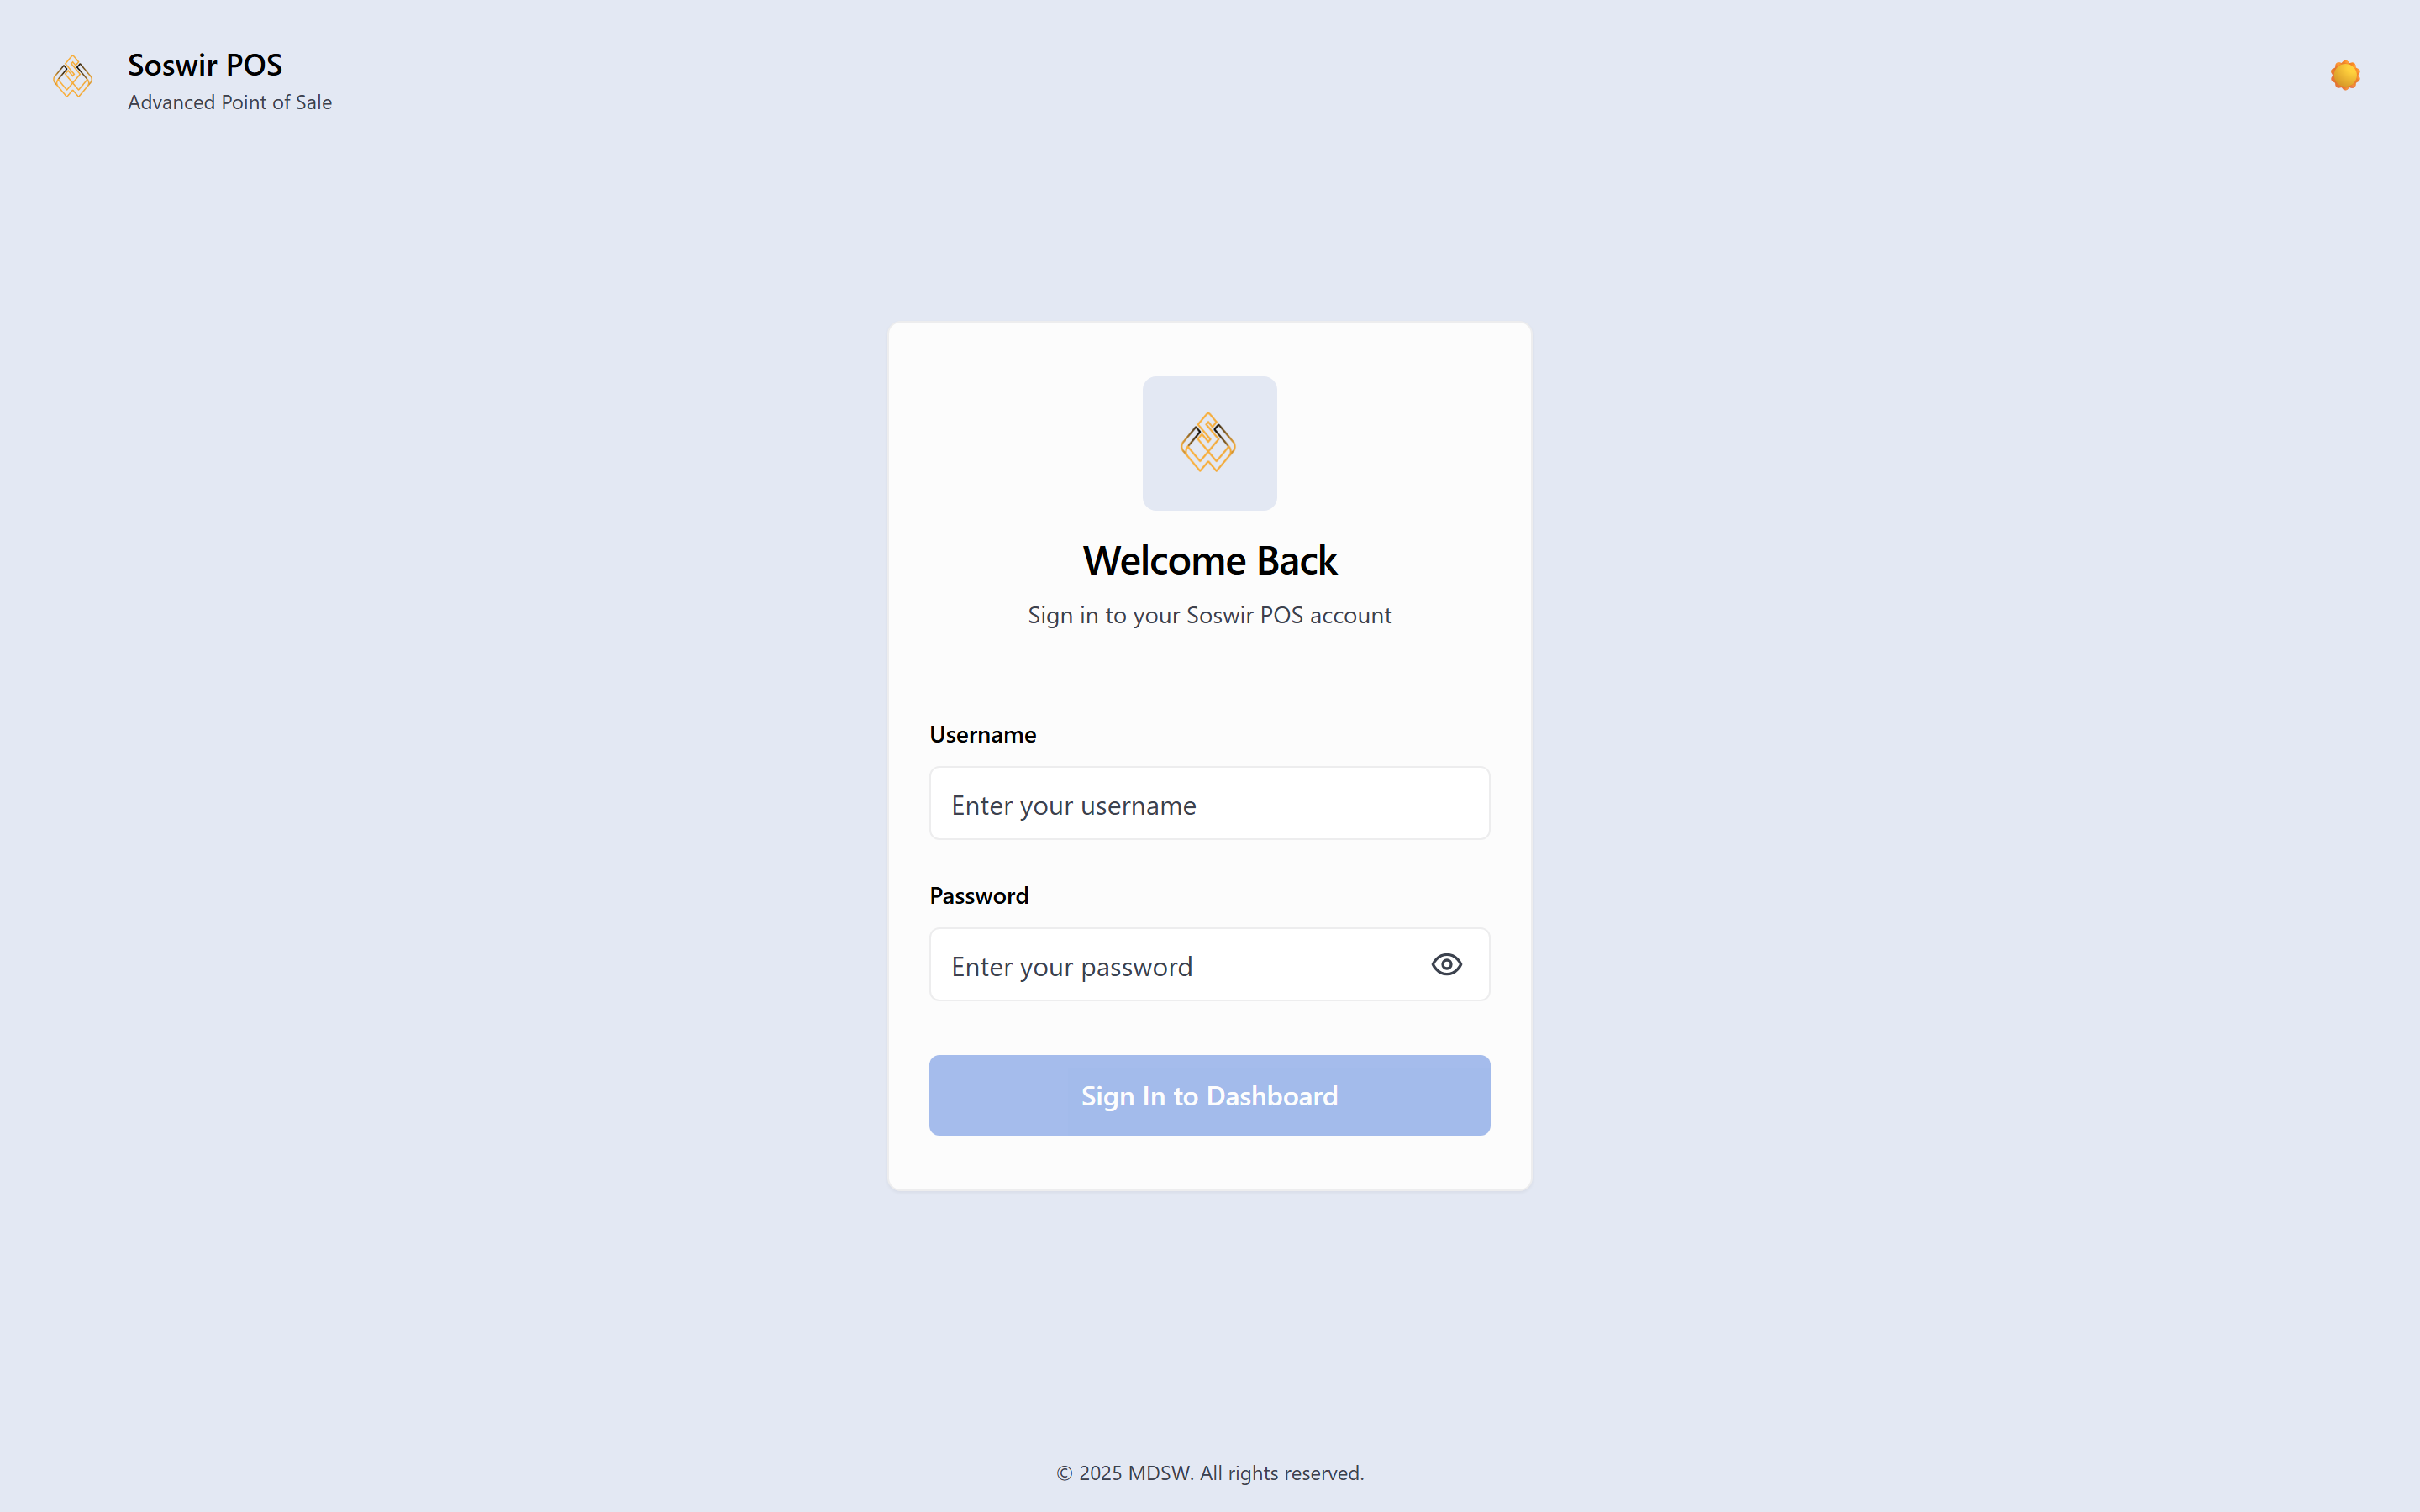
\includegraphics[width=0.99\linewidth,height=0.40\textheight,keepaspectratio,cfbox=garis 0.5pt 0pt]{img/01-login.png}
\caption{Halaman masuk akun.}
\end{figure}

\subsection{Kasir hanya bisa masuk pada jam shift}

Setiap kasir ditempatkan di satu sesi shift, misalnya \ui{Sesi 1} pukul 10:00--17:00. Kasir hanya bisa masuk pada rentang jam sesinya, dengan kelonggaran 15 menit sebelum jam mulai dan 15 menit sesudah jam selesai. Di luar itu, aplikasi menolak dan menampilkan jadwal kasir tersebut.

\begin{figure}[H]
\centering
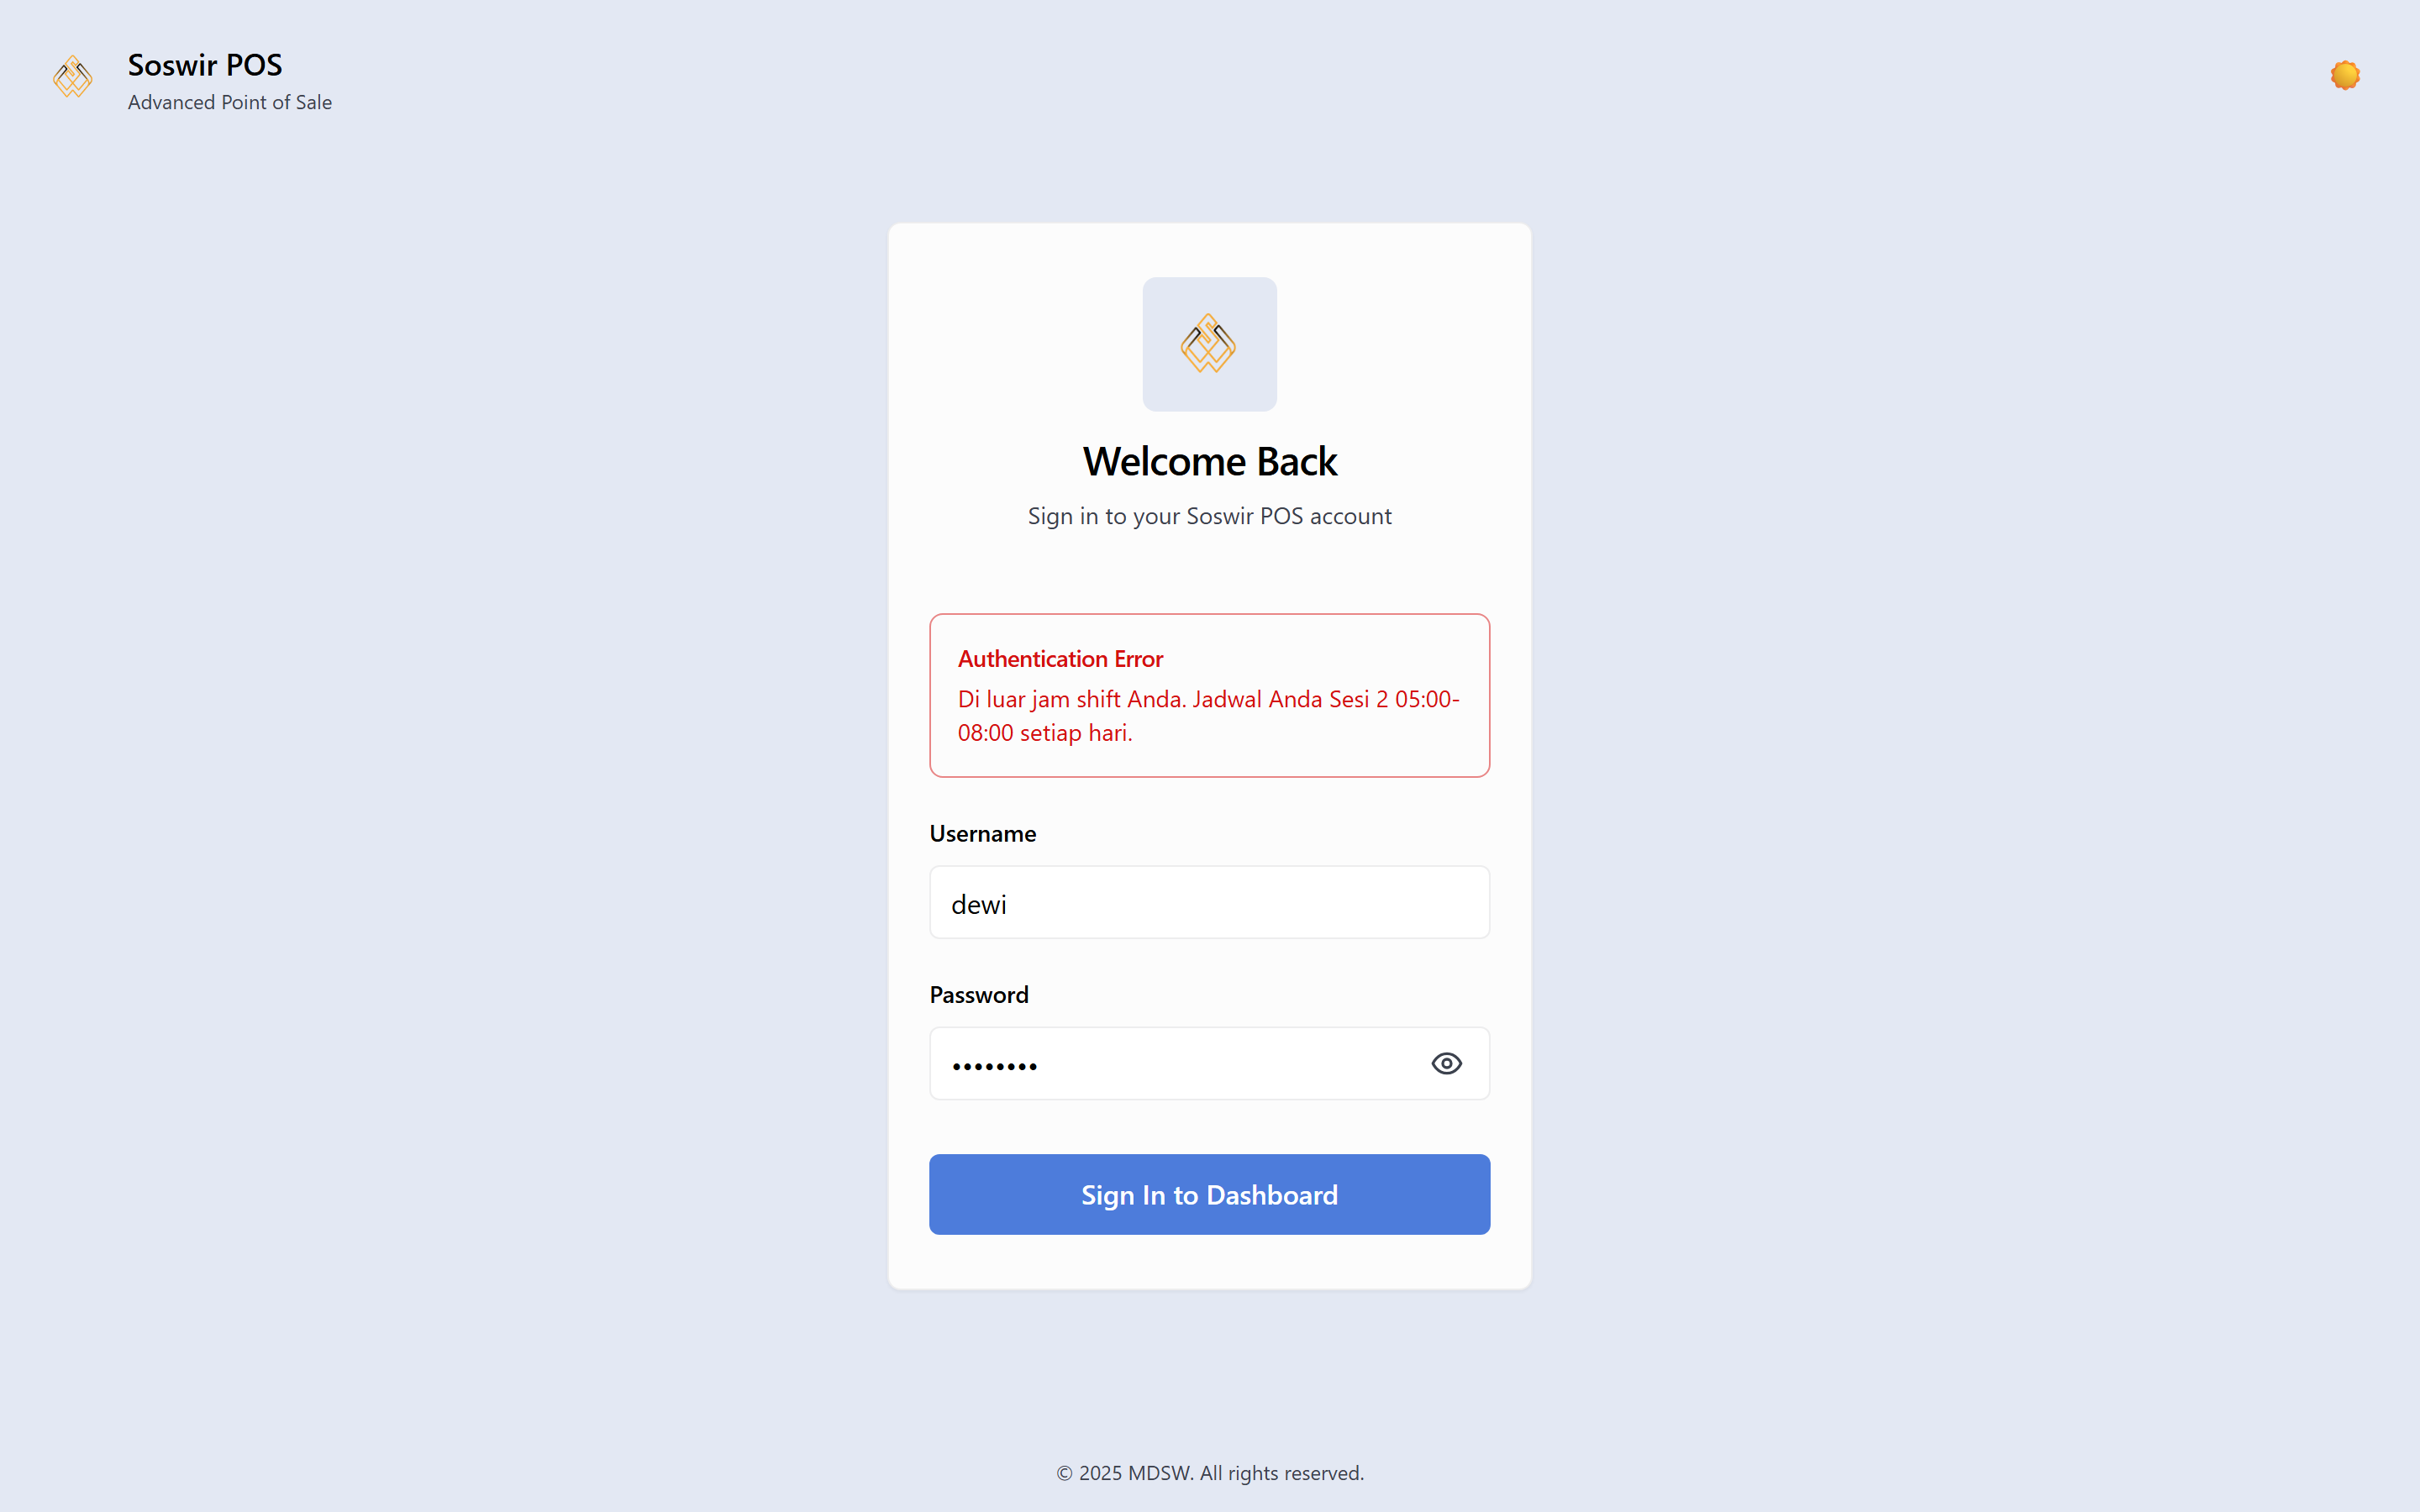
\includegraphics[width=0.99\linewidth,height=0.40\textheight,keepaspectratio,cfbox=garis 0.5pt 0pt]{img/02-login-di-luar-shift.png}
\caption{Kasir yang mencoba masuk di luar jam shift mendapat pesan ``Di luar jam shift Anda'' beserta jadwalnya.}
\end{figure}

\begin{catatan}
Kalau shift habis saat kasir masih membuka aplikasi, kasir otomatis dikeluarkan dan halaman masuk menampilkan pesan yang sama. Kasir yang belum ditempatkan di sesi mana pun mendapat pesan ``Anda belum ditempatkan di sesi shift mana pun. Hubungi superadmin.'' Superadmin tidak dibatasi jam.
\end{catatan}

\subsection{Keluar dari akun}

\begin{enumerate}
  \item Tekan nama Anda di pojok kanan atas.
  \item Pilih \ui{Logout}. Anda kembali ke halaman masuk.
\end{enumerate}

\begin{figure}[H]
\centering
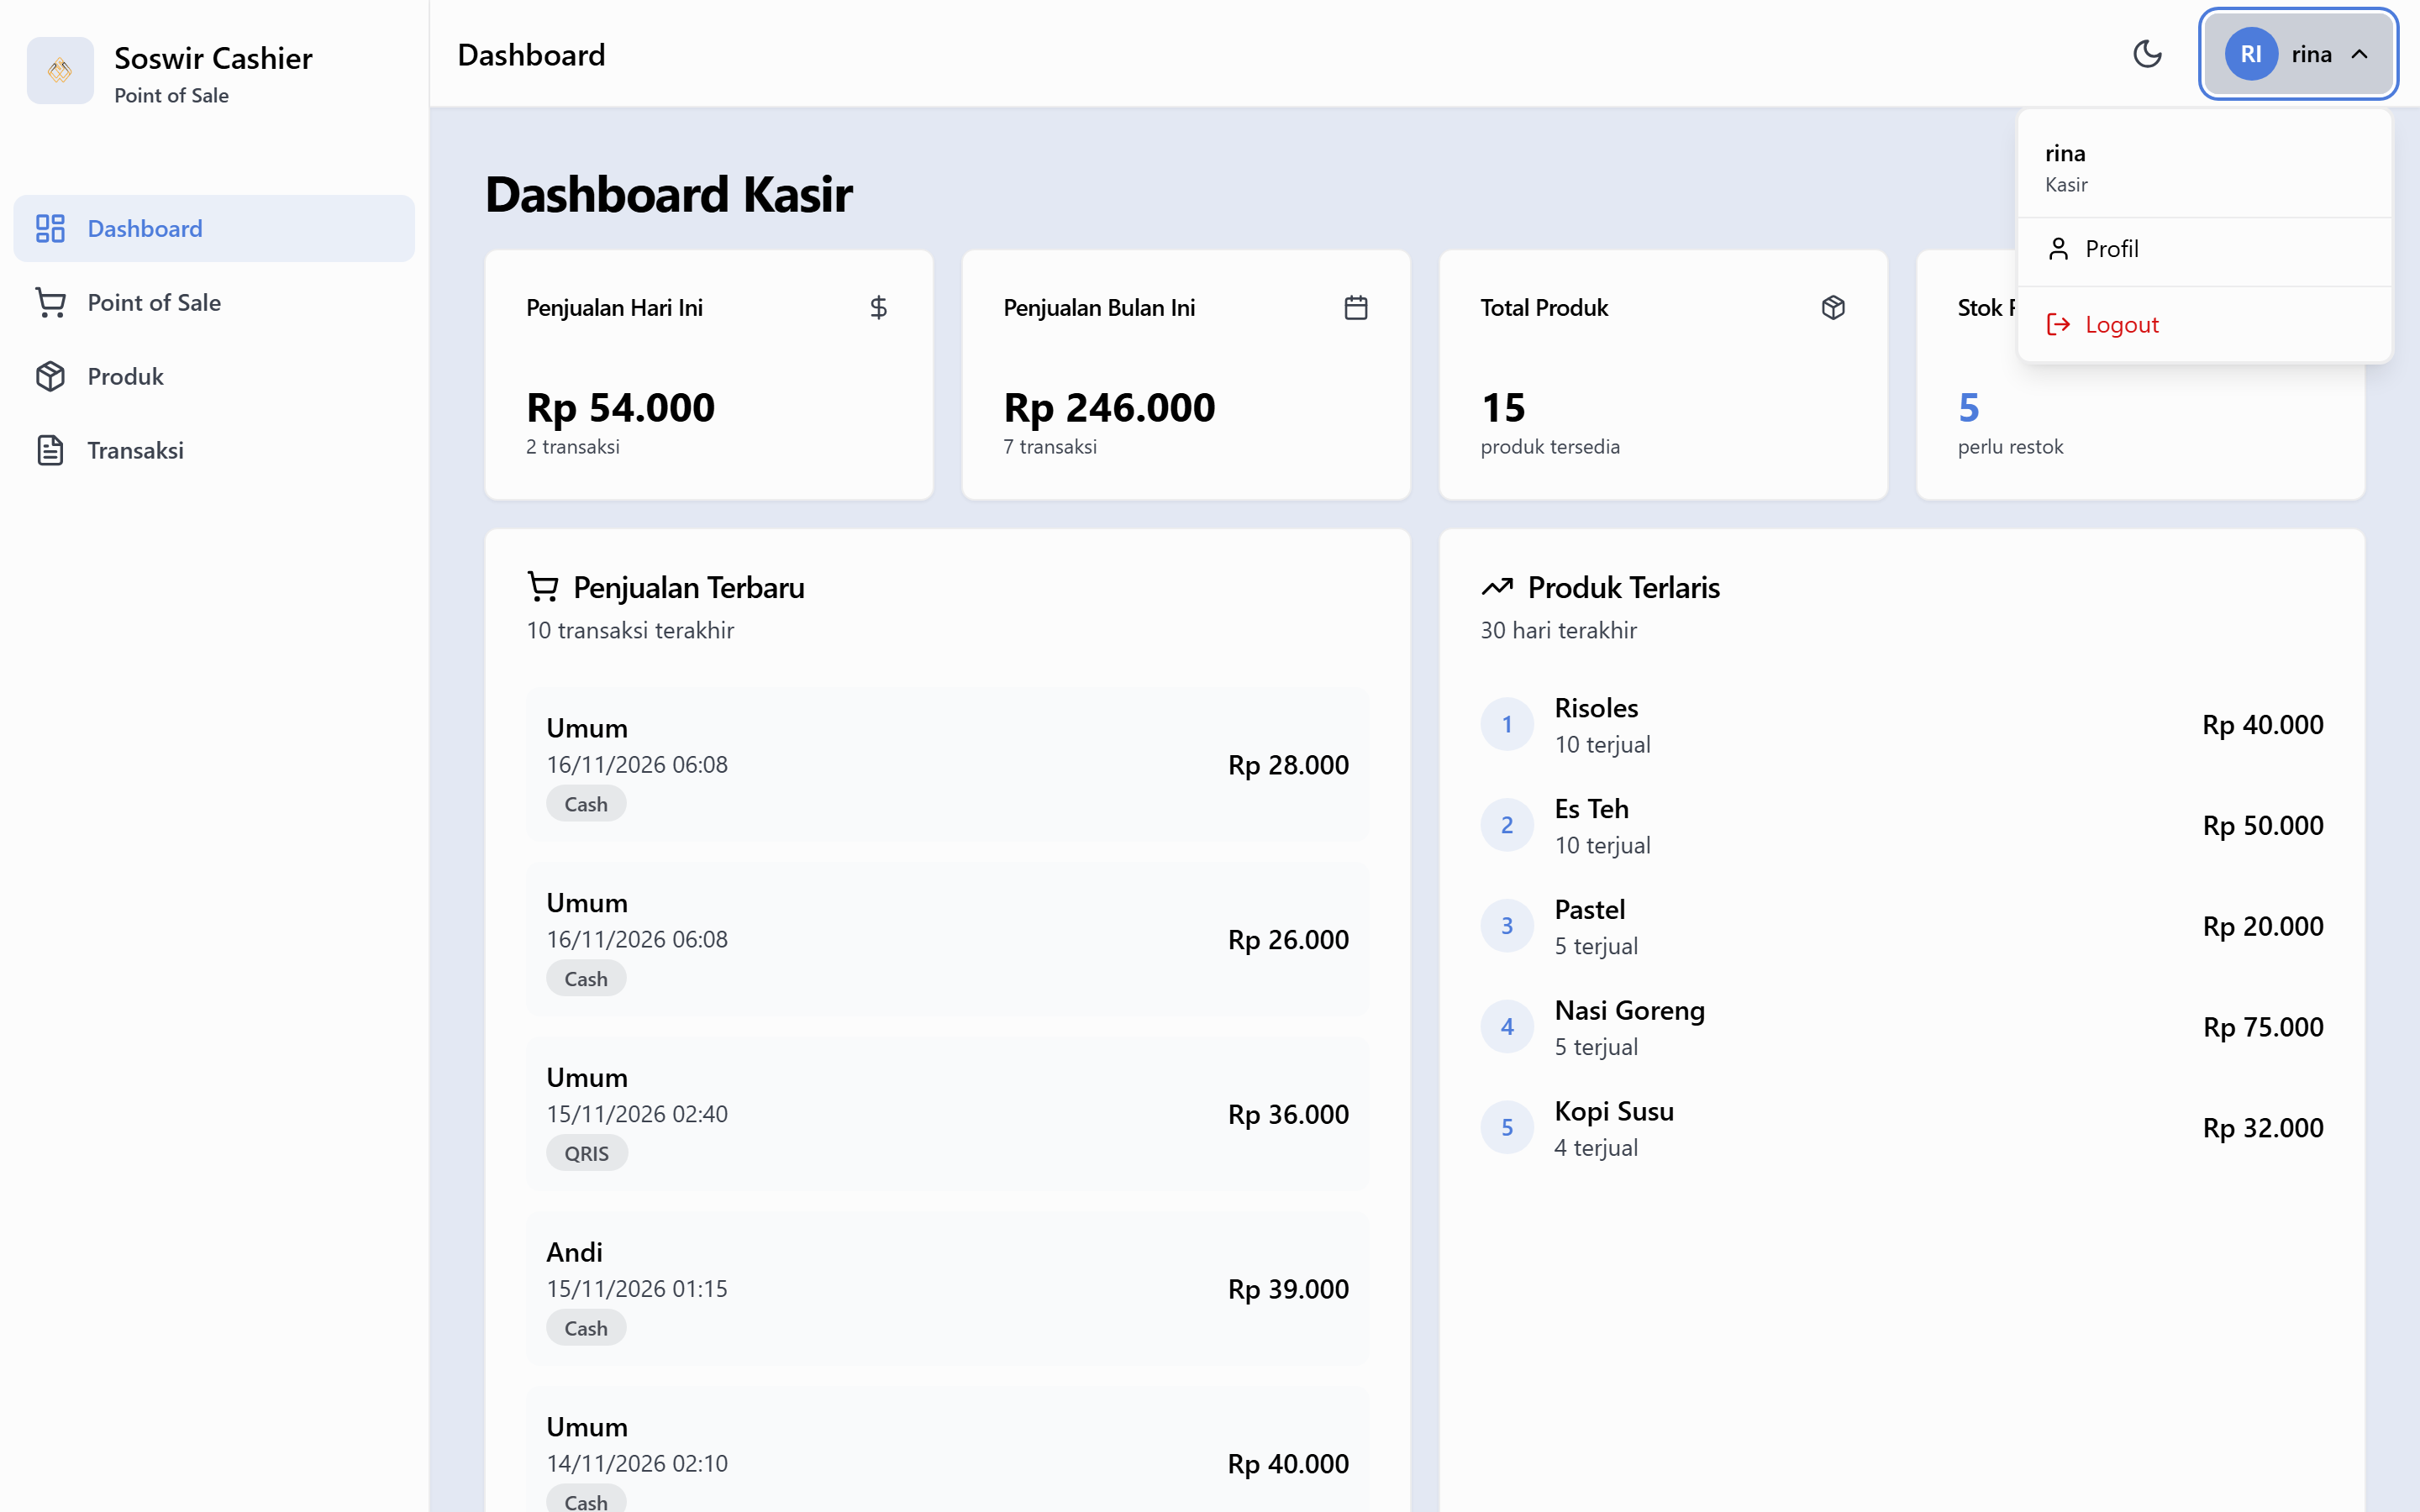
\includegraphics[width=0.99\linewidth,height=0.40\textheight,keepaspectratio,cfbox=garis 0.5pt 0pt]{img/04-menu-akun.png}
\caption{Menu akun di pojok kanan atas berisi \ui{Profil} dan \ui{Logout}. Pada akun superadmin ada juga \ui{Pengaturan}.}
\end{figure}

Selalu keluar dari akun sebelum meninggalkan komputer kasir, terutama saat pergantian shift.

\subsection{Mengubah username dan password}

Kasir dan superadmin bisa mengganti username dan password-nya sendiri.

\begin{enumerate}
  \item Tekan nama Anda di pojok kanan atas, lalu pilih \ui{Profil}.
  \item Ubah \ui{Username} bila perlu.
  \item Untuk mengganti password, isi \ui{Password Lama}, \ui{Password Baru}, dan \ui{Konfirmasi Password Baru}. Biarkan ketiganya kosong kalau tidak ingin mengganti password.
  \item Tekan \ui{Simpan Perubahan}.
\end{enumerate}

\begin{figure}[H]
\centering
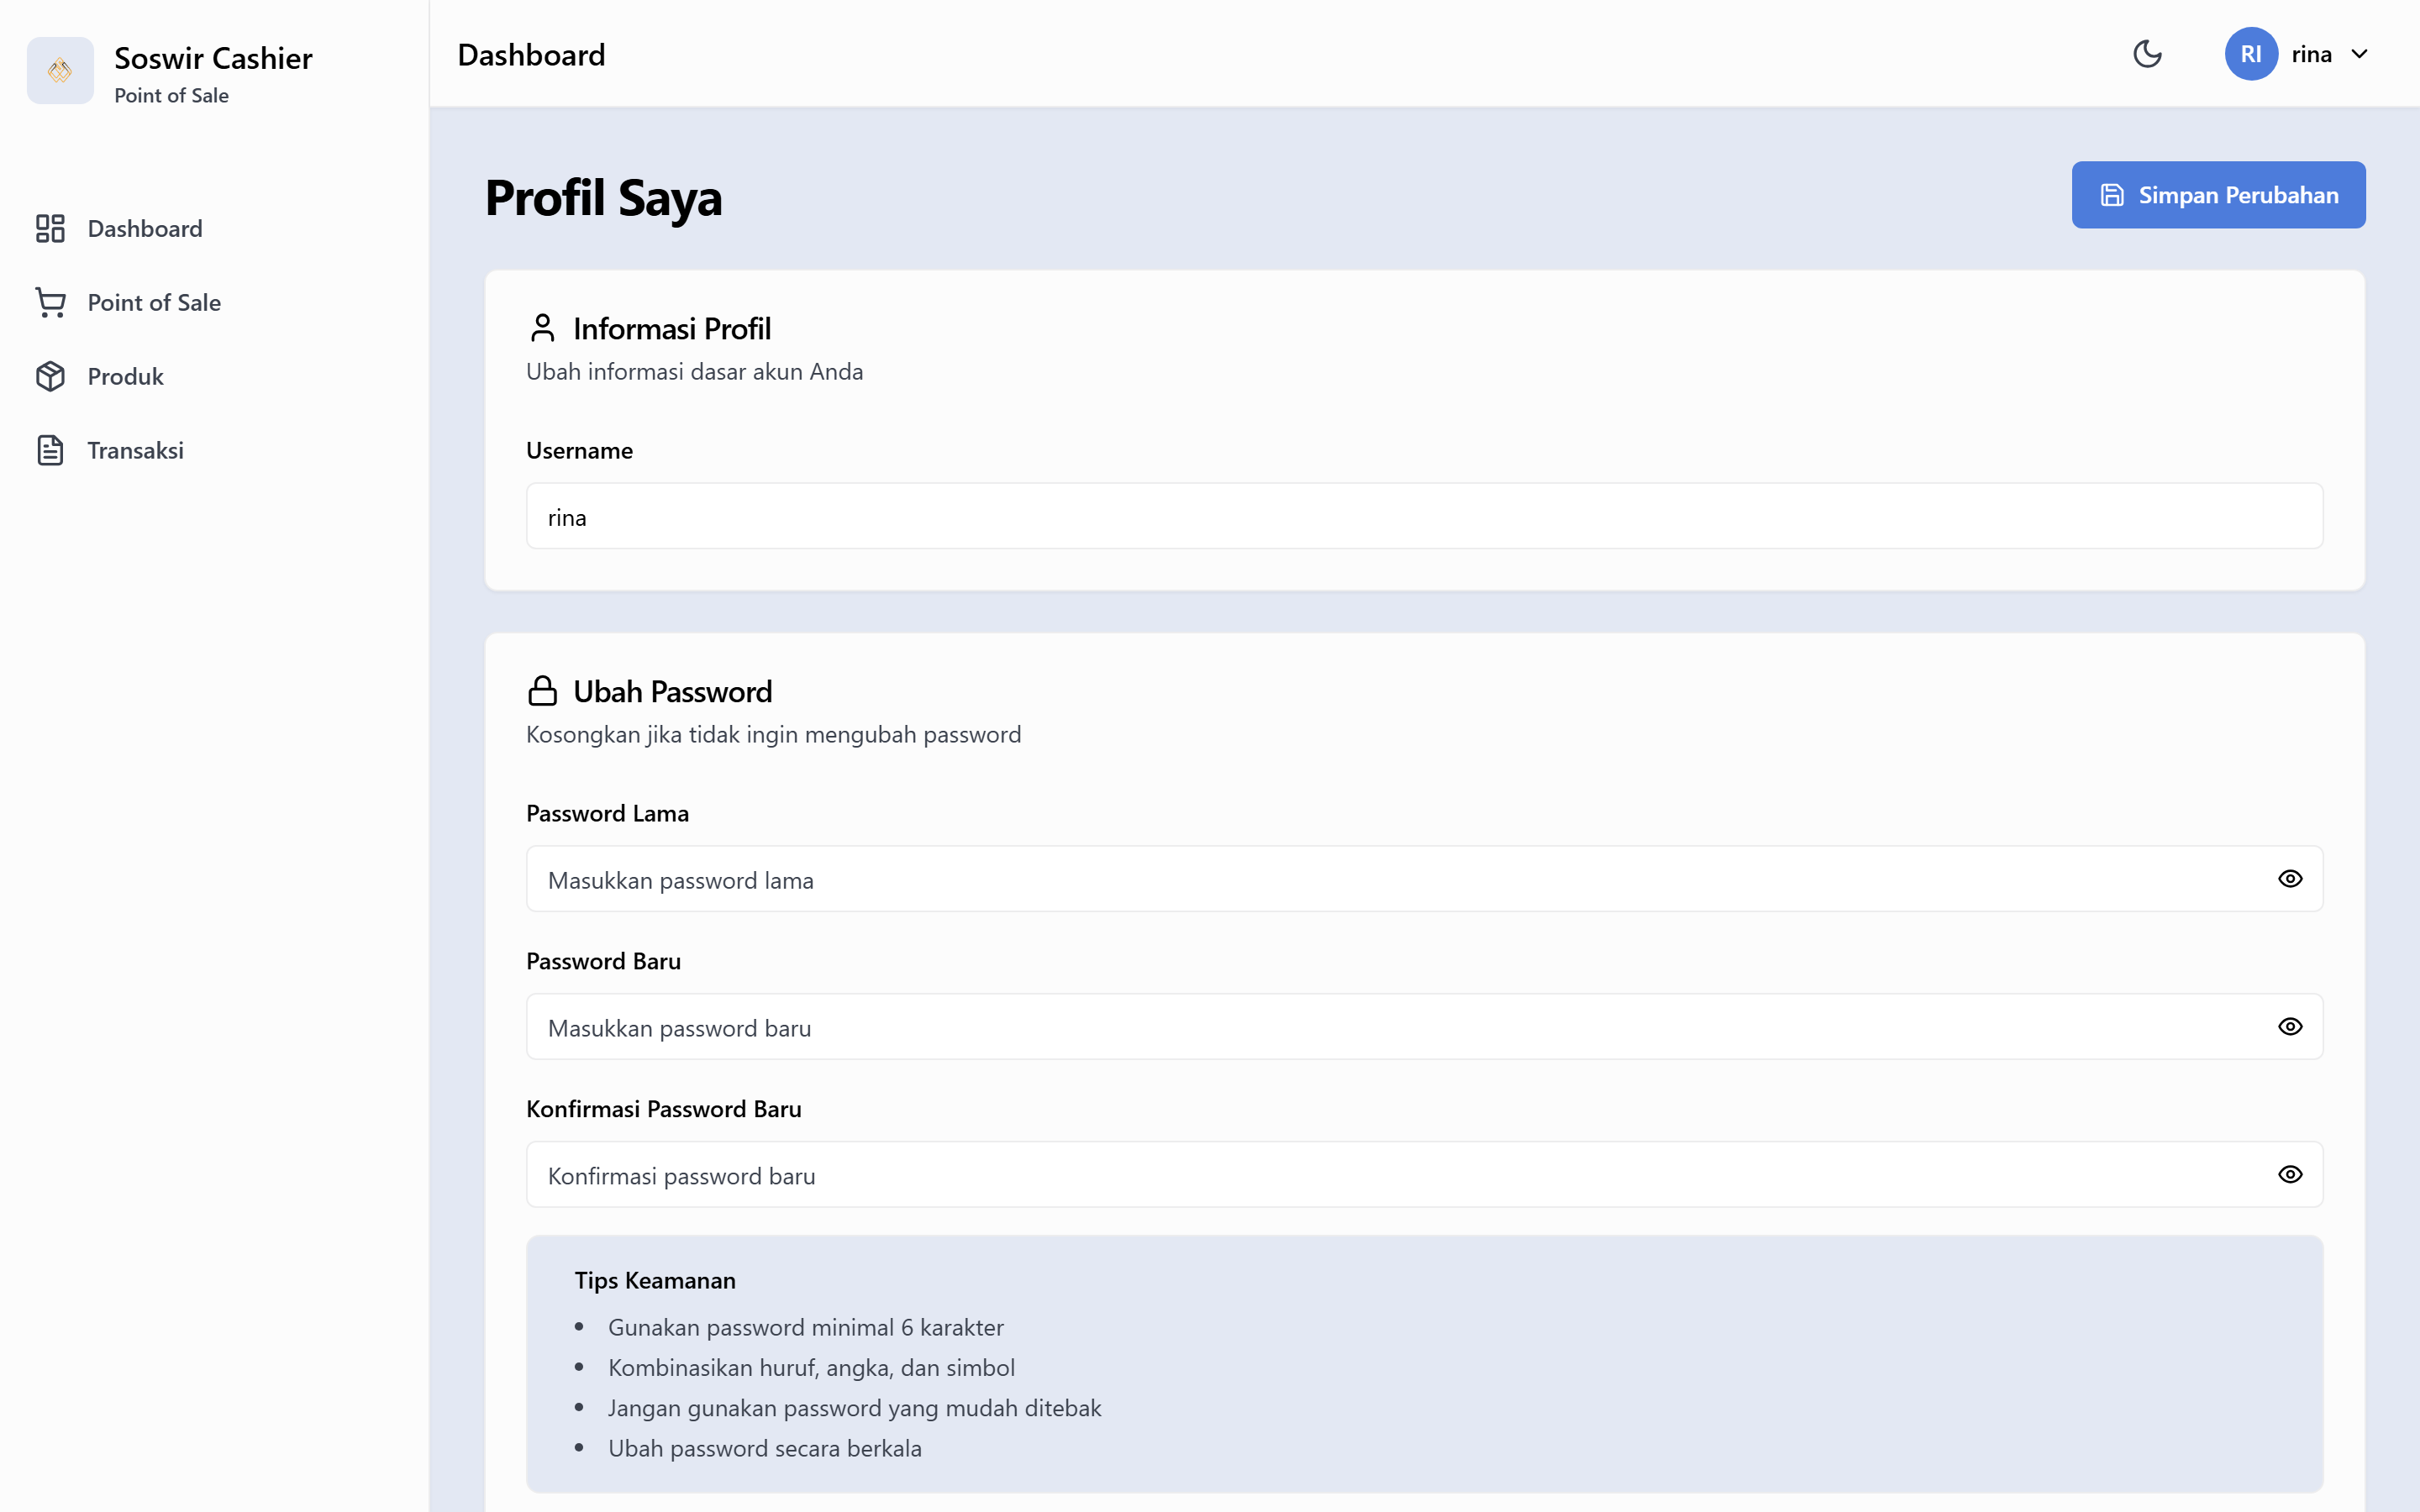
\includegraphics[width=0.99\linewidth,height=0.40\textheight,keepaspectratio,cfbox=garis 0.5pt 0pt]{img/12-profil.png}
\caption{Halaman \ui{Profil Saya}.}
\end{figure}

% ---------------------------------------------------------------
\section{Kasir}

Menu kasir ada di sisi kiri: \ui{Dashboard}, \ui{Point of Sale}, \ui{Produk}, dan \ui{Transaksi}.

\subsection{Dashboard kasir}

Halaman ini terbuka setelah kasir masuk. Isinya ringkasan singkat untuk kasir.

\begin{figure}[H]
\centering
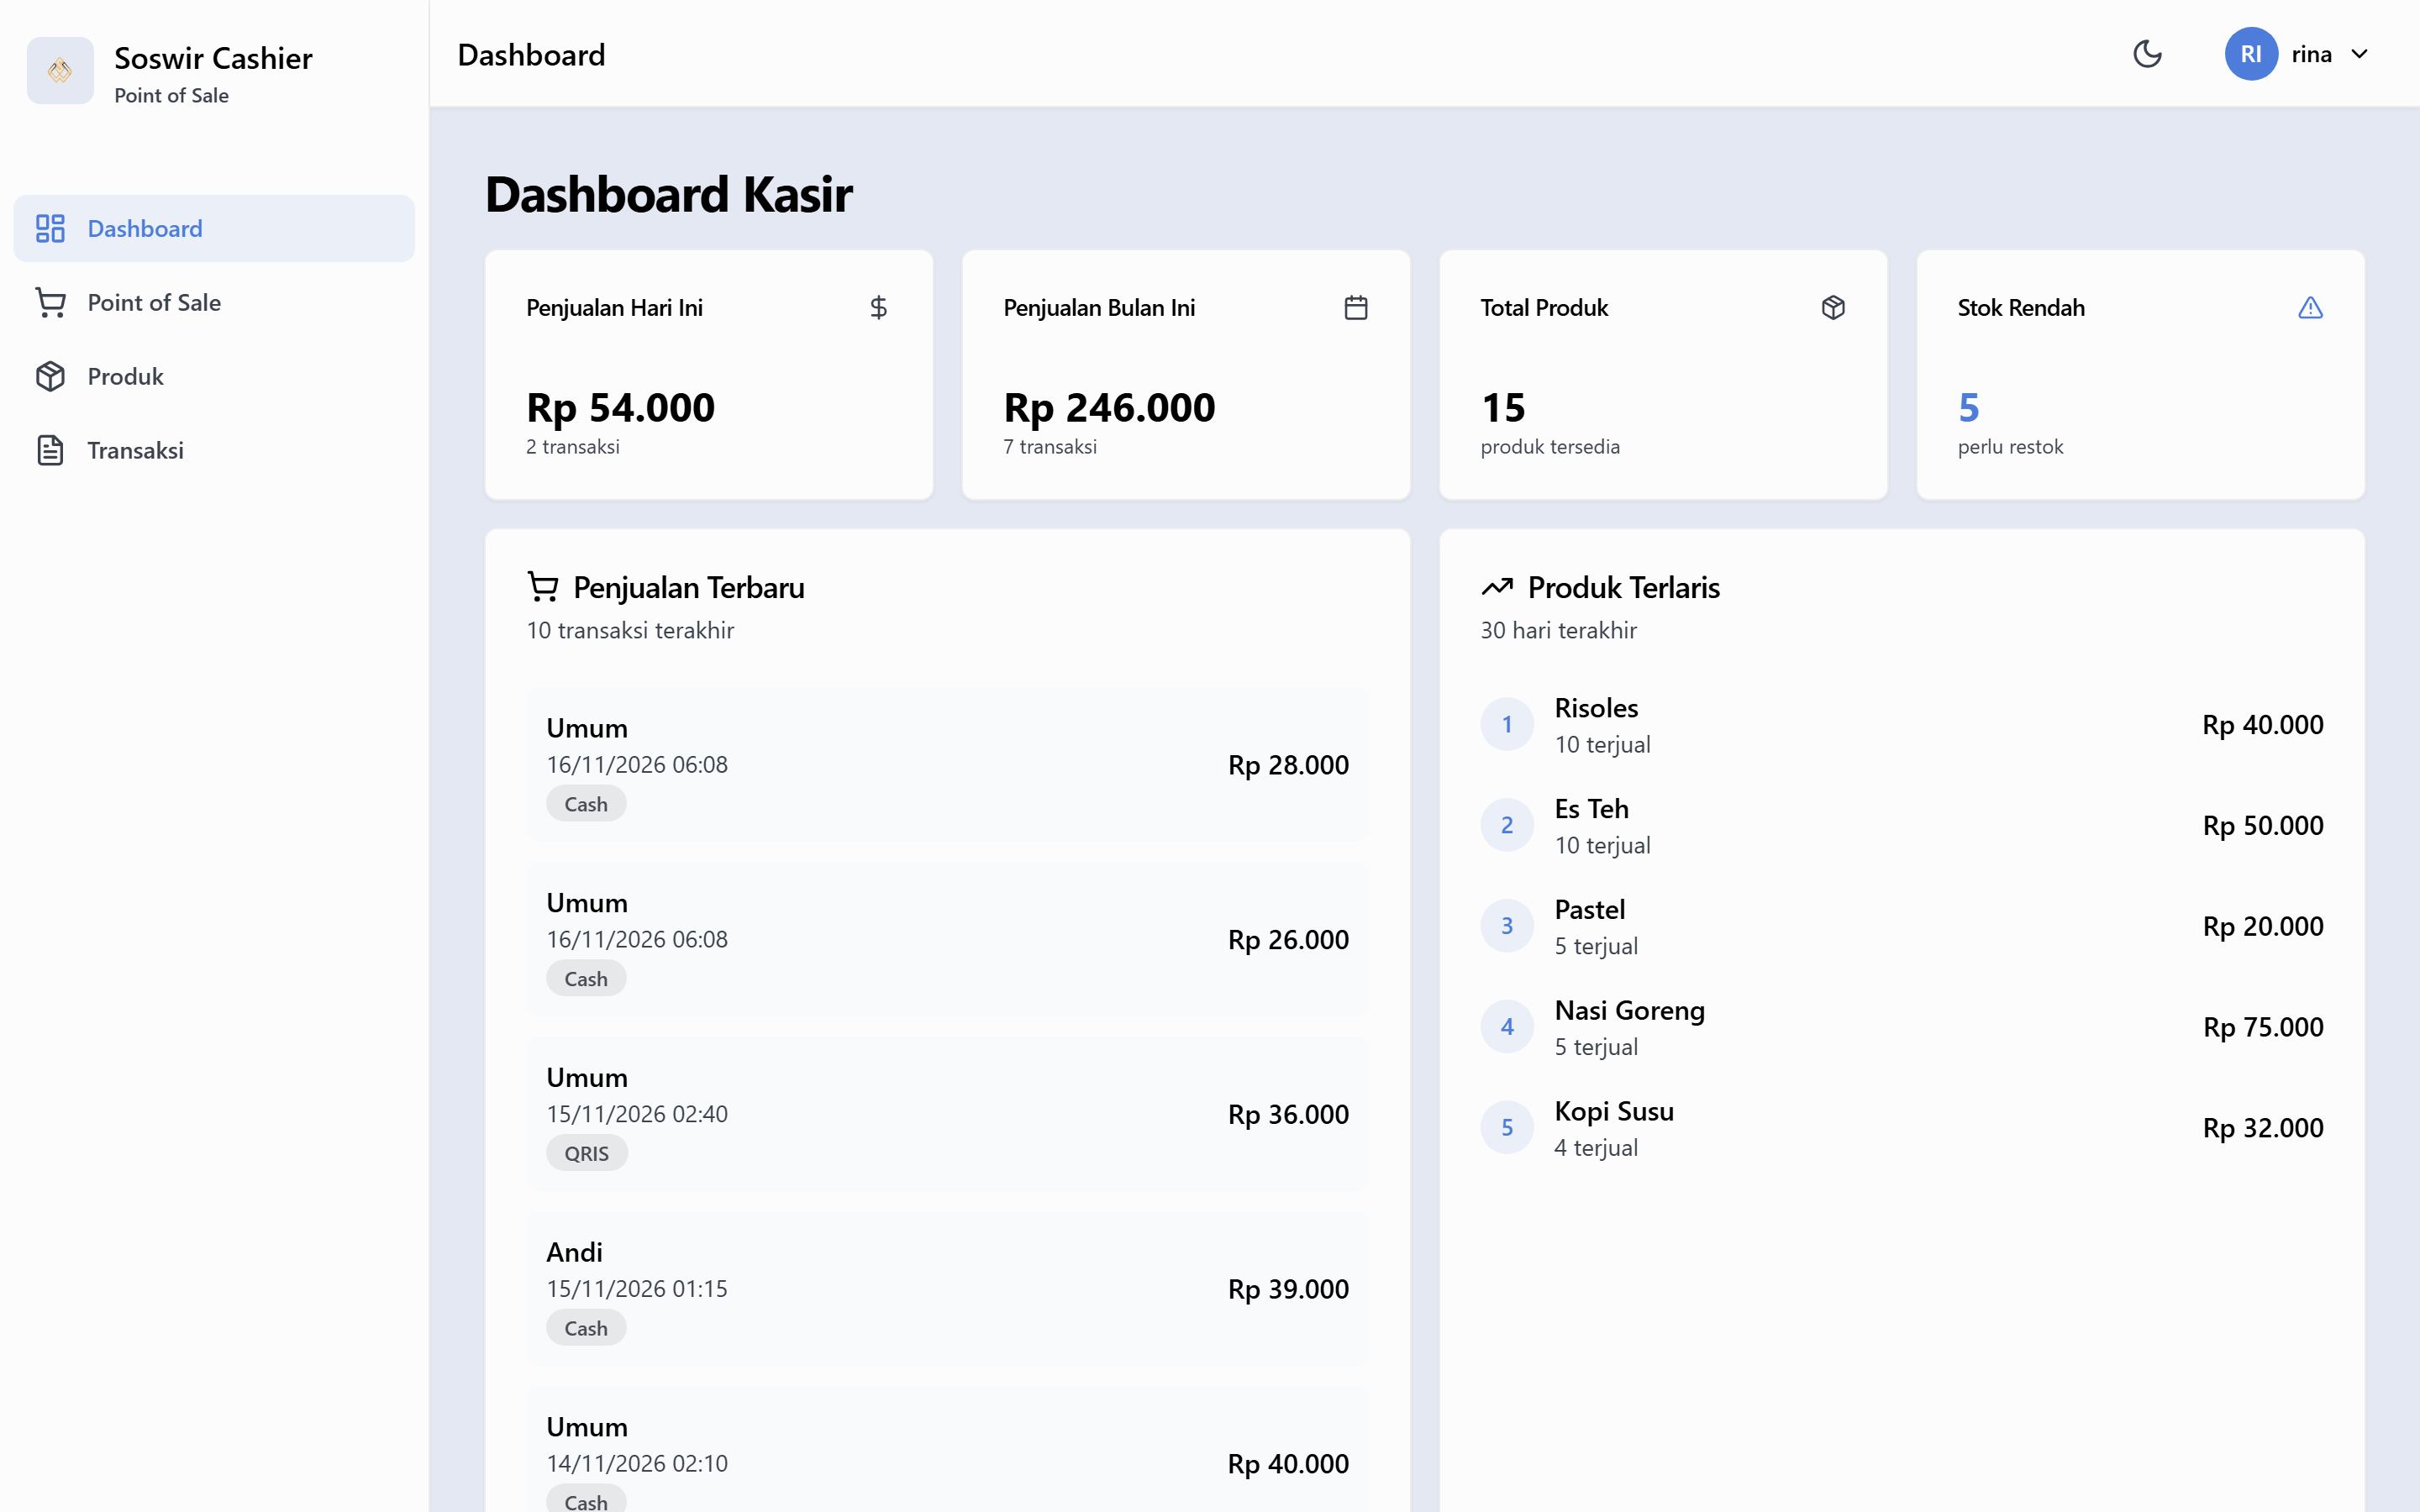
\includegraphics[width=0.99\linewidth,height=0.40\textheight,keepaspectratio,cfbox=garis 0.5pt 0pt]{img/03-kasir-dashboard.png}
\caption{\ui{Dashboard Kasir}.}
\end{figure}

\begin{itemize}
  \item \ui{Penjualan Hari Ini} dan \ui{Penjualan Bulan Ini}: total uang penjualan dan jumlah transaksinya.
  \item \ui{Total Produk} dan \ui{Stok Rendah}: jumlah produk dan berapa yang stoknya menipis.
  \item \ui{Penjualan Terbaru}: 10 transaksi terakhir.
  \item \ui{Produk Terlaris}: produk paling laku dalam 30 hari terakhir.
  \item Di bagian bawah ada \ui{Produk Stok Rendah} dan tabel \ui{Stok PUBJ} untuk barang titipan.
\end{itemize}

\subsection{Melayani penjualan}

Semua penjualan dicatat di menu \ui{Point of Sale}.

\begin{enumerate}
  \item Tekan \ui{Point of Sale} di menu kiri.
  \item Cari produk lewat kotak \ui{Cari produk...}, atau pilih kategori di daftar \ui{Semua Kategori}.
  \item Tekan \ui{Tambah ke Keranjang} pada produk yang dibeli. Produk masuk ke \ui{Keranjang Belanja} di sebelah kanan.
\end{enumerate}

\begin{figure}[H]
\centering
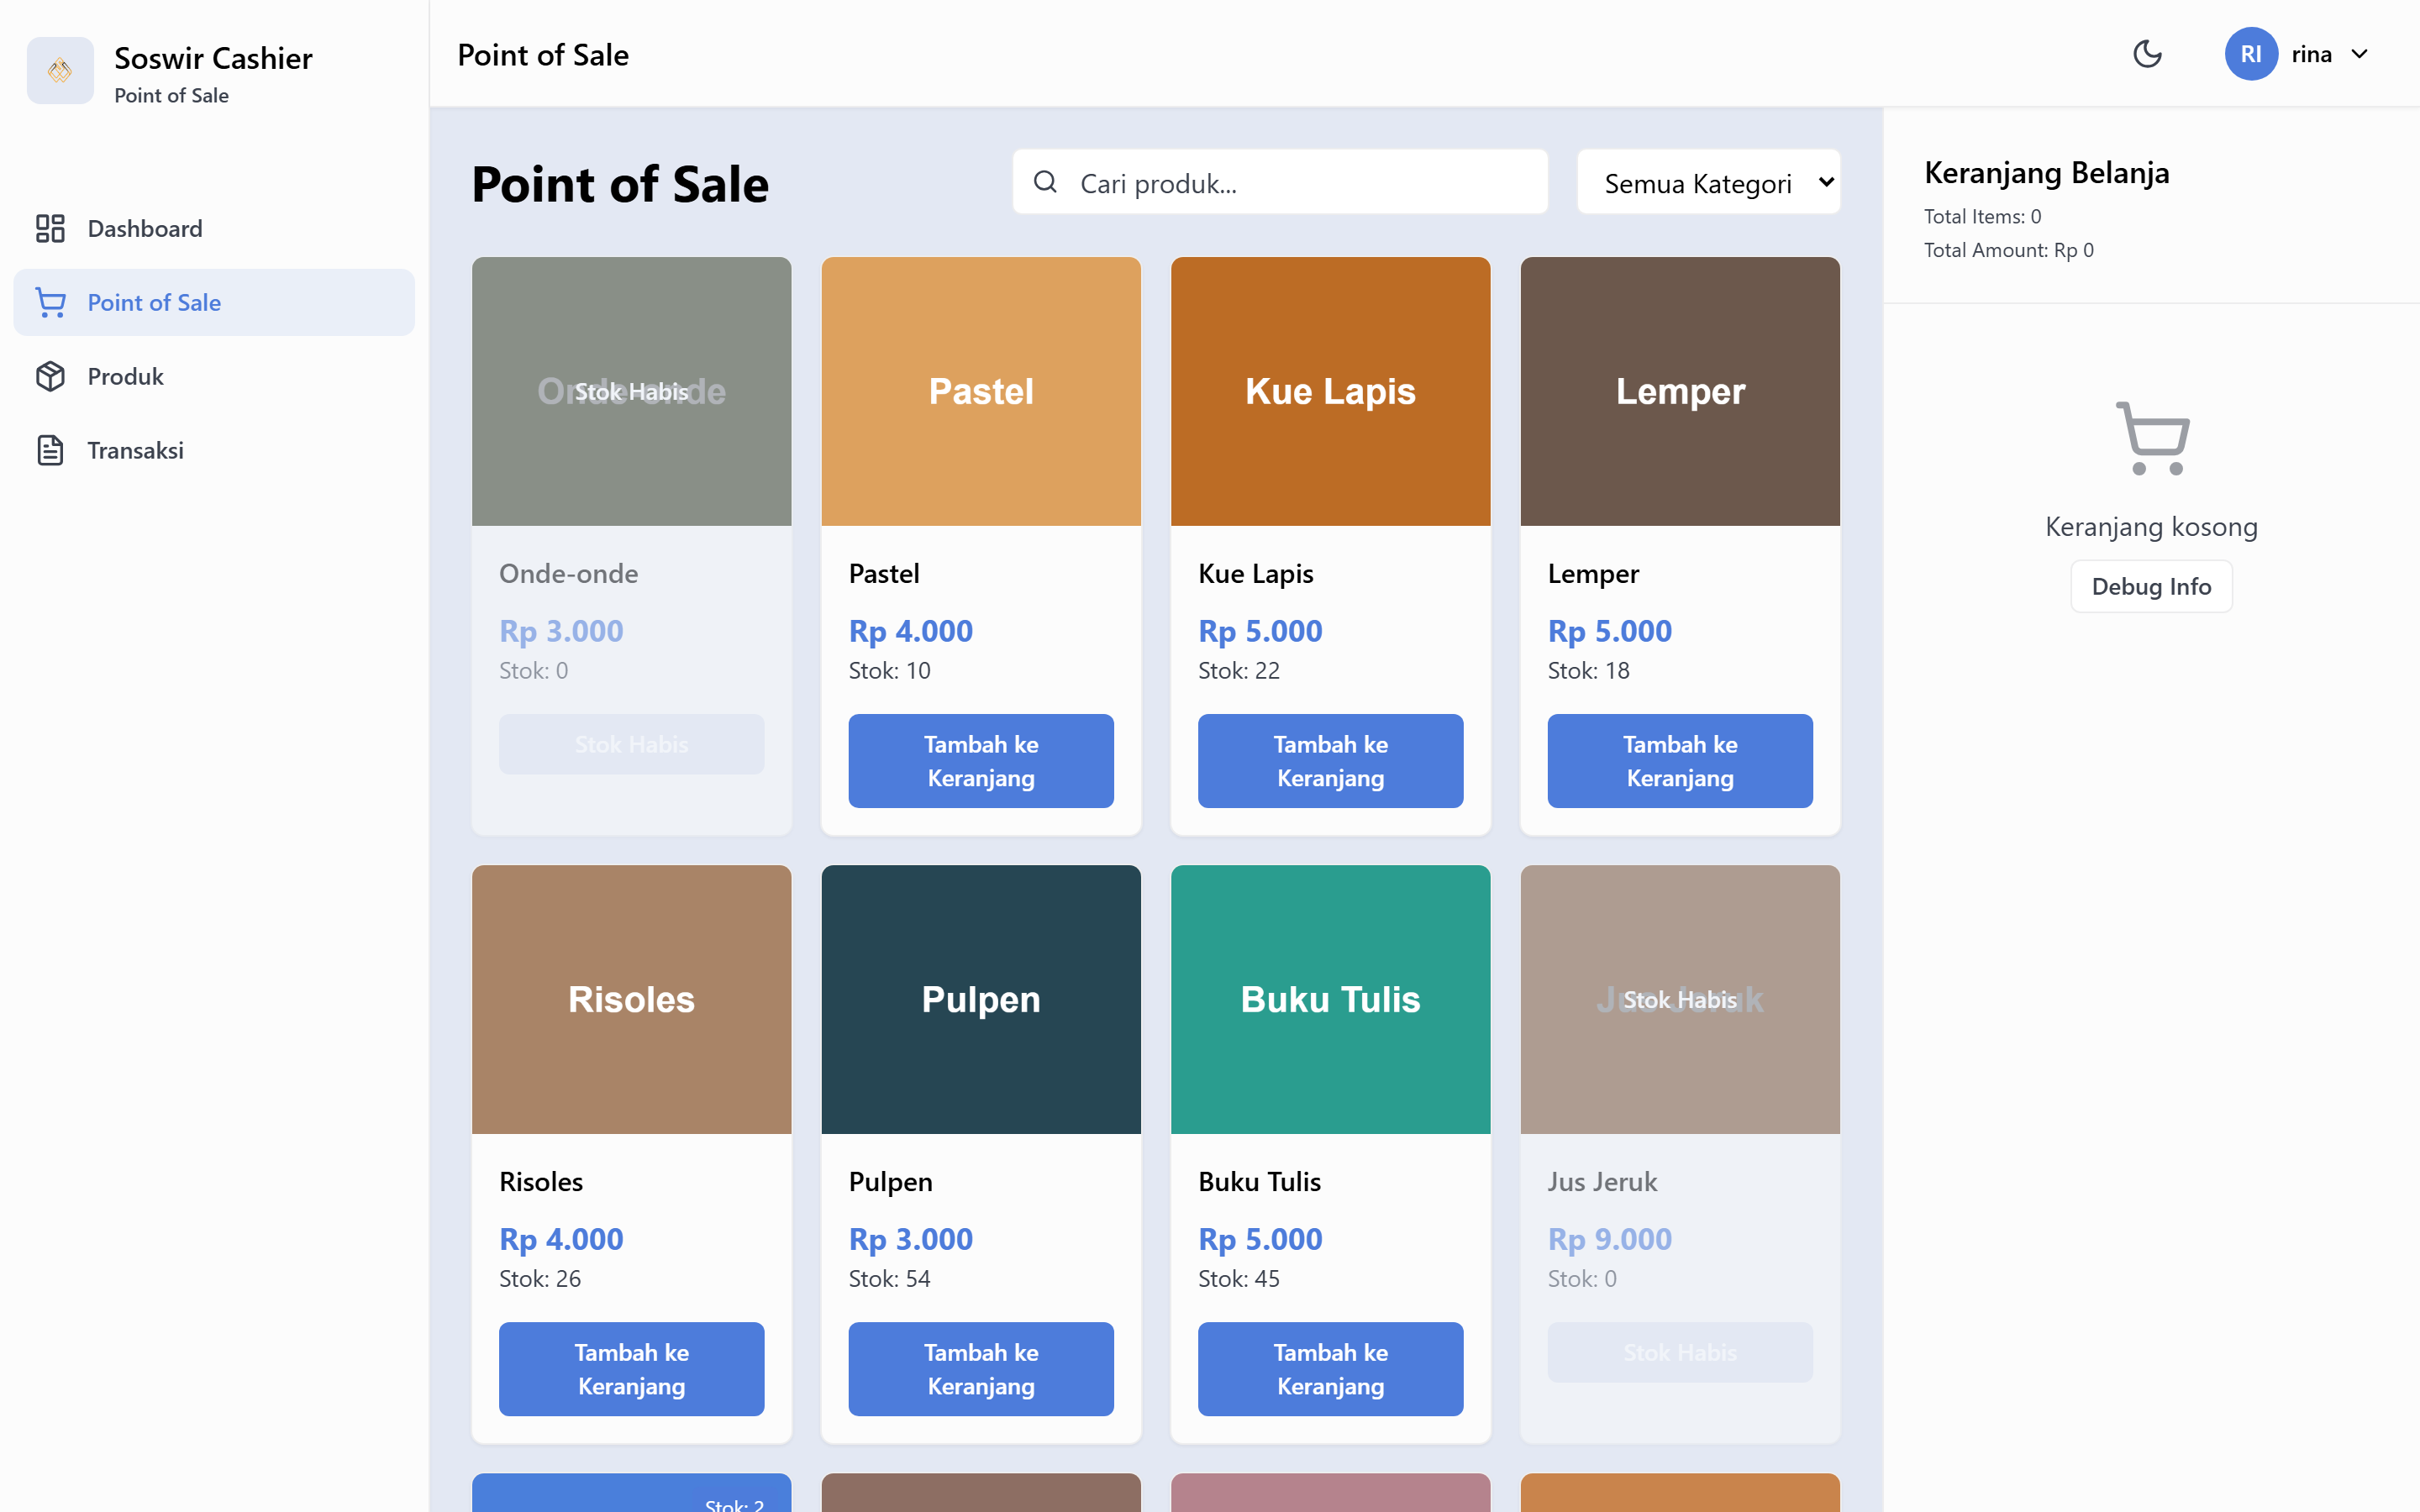
\includegraphics[width=0.99\linewidth,height=0.40\textheight,keepaspectratio,cfbox=garis 0.5pt 0pt]{img/05-pos-katalog.png}
\caption{Halaman \ui{Point of Sale}. Kartu produk menampilkan harga dan sisa stok.}
\end{figure}

\clearpage
\begin{enumerate}[resume]
  \item Atur jumlah di keranjang dengan tombol \ui{+} dan \ui{−}. Jumlah yang diturunkan sampai nol menghapus produk dari keranjang. Tombol \ui{Kosongkan Keranjang} di bawah keranjang menghapus semua isinya.
  \item Periksa \ui{Total:} di bawah keranjang, lalu tekan \ui{Checkout}.
\end{enumerate}

\begin{figure}[H]
\centering
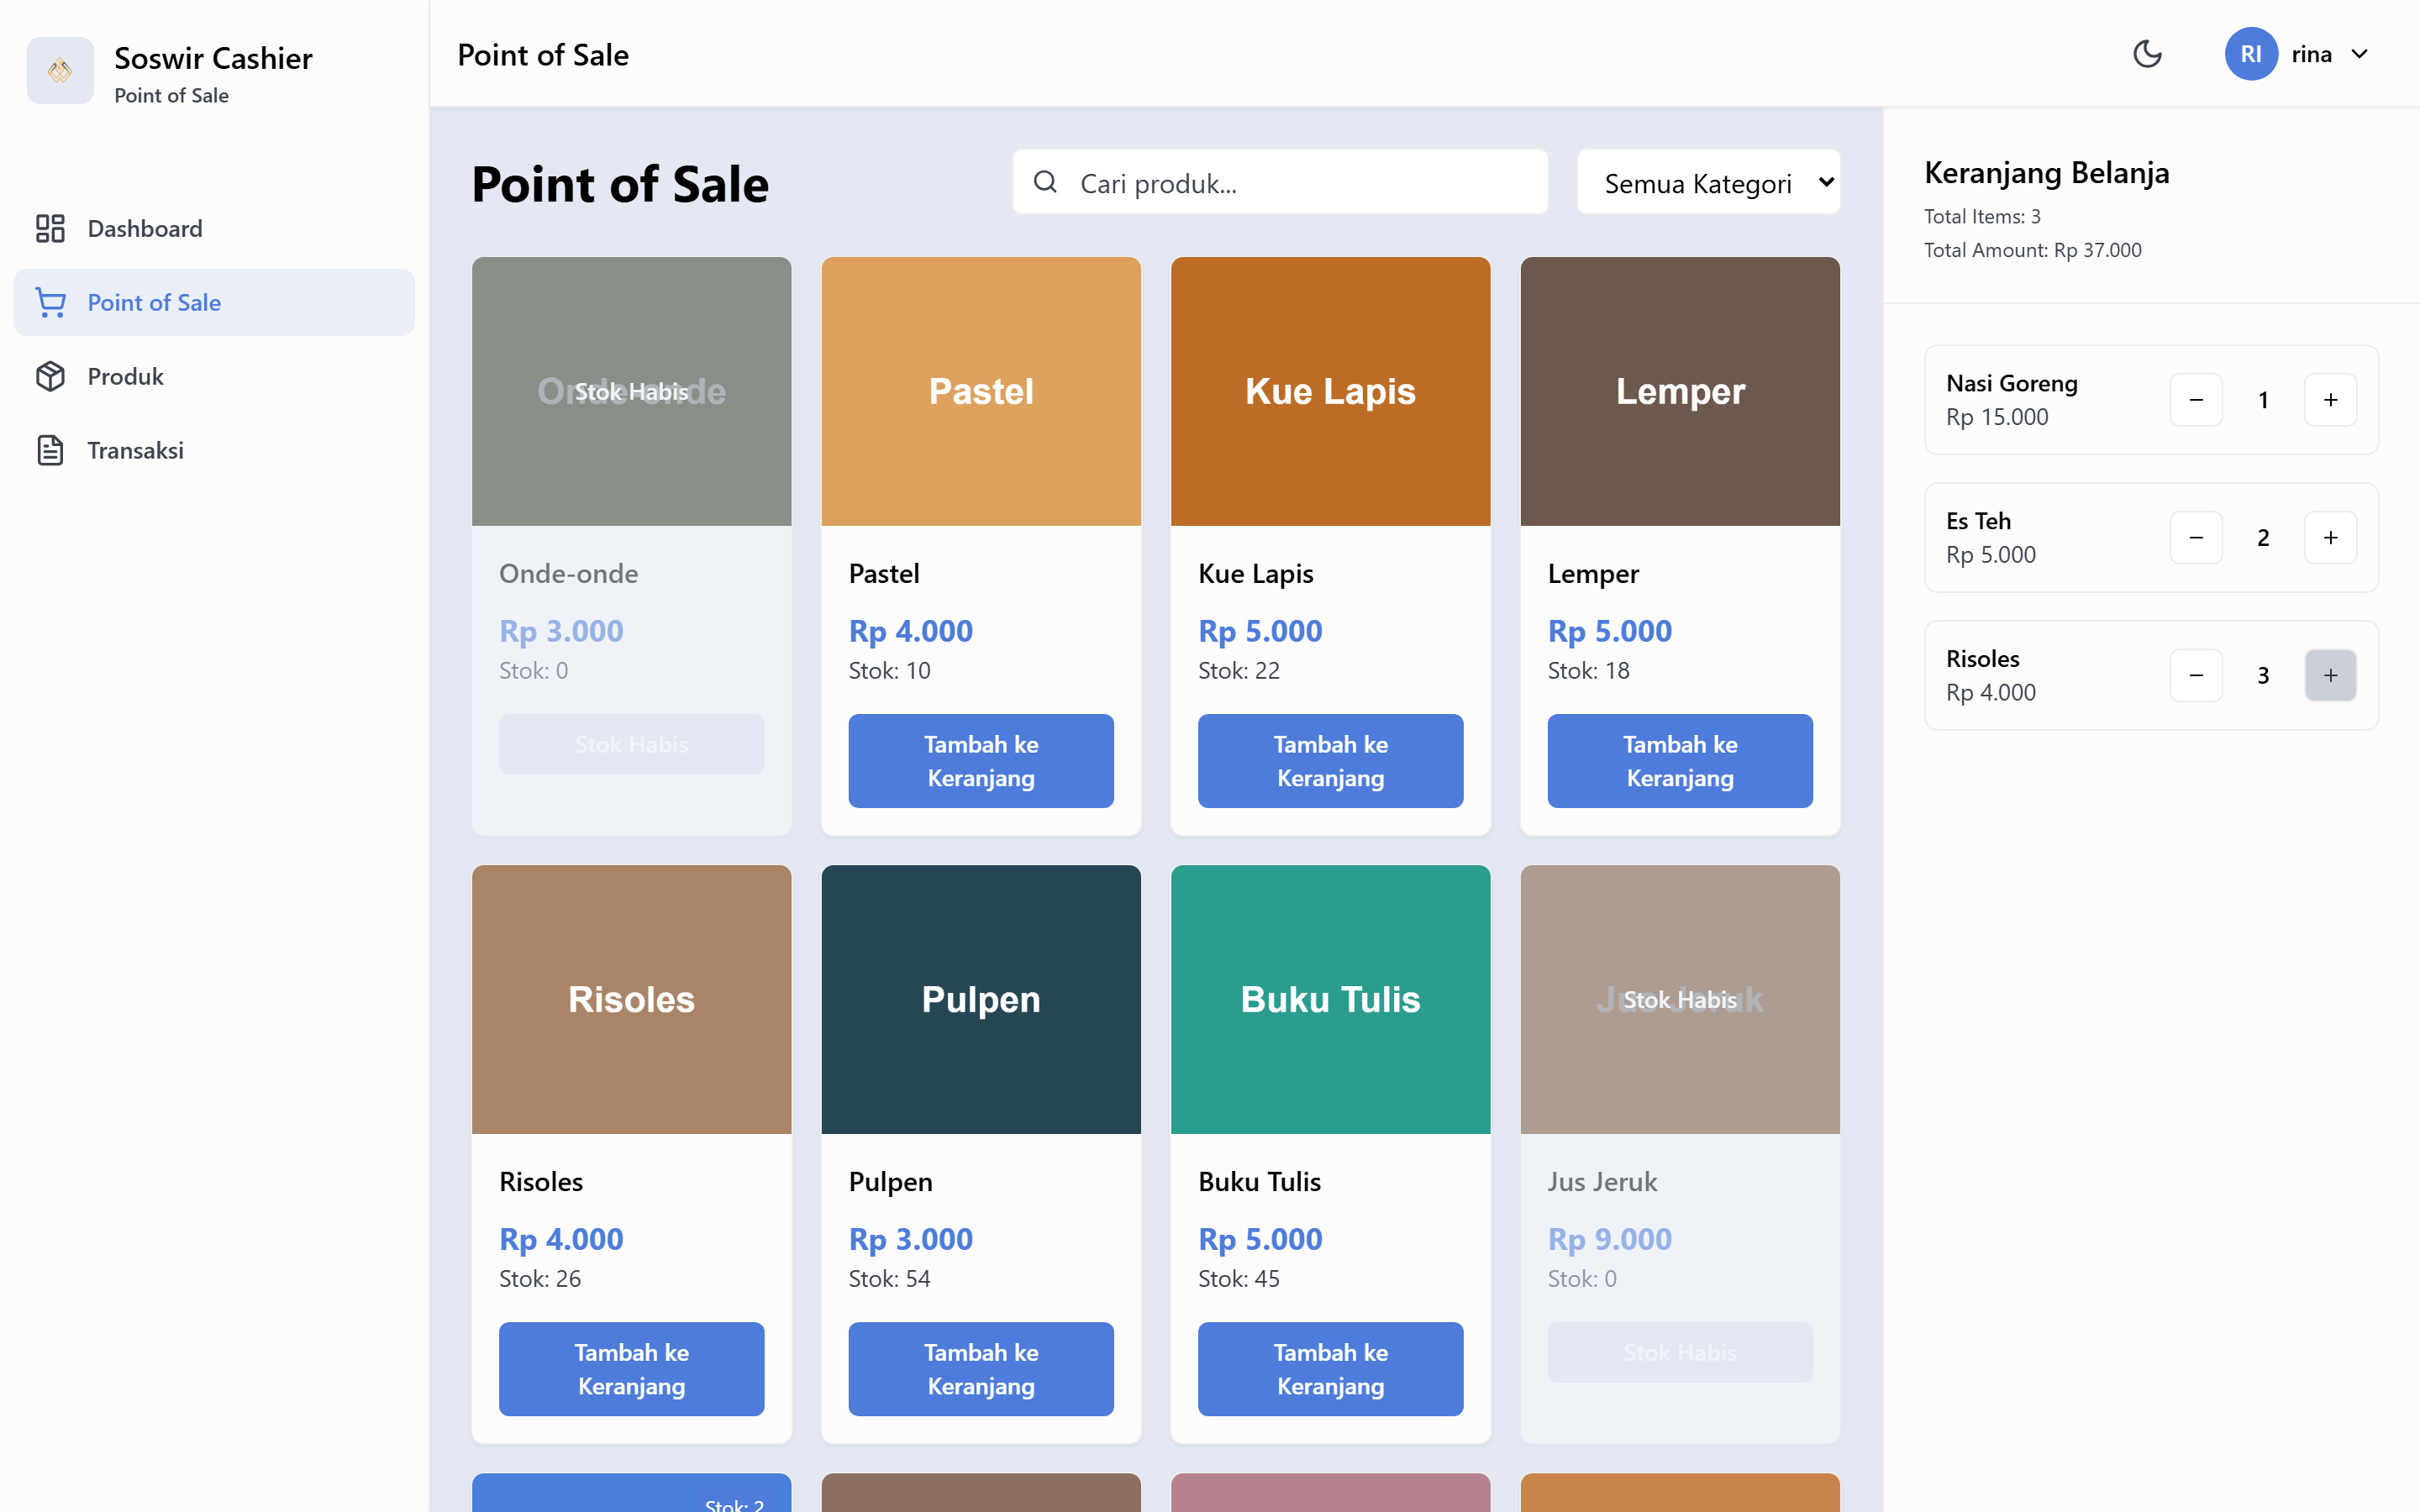
\includegraphics[width=0.99\linewidth,height=0.40\textheight,keepaspectratio,cfbox=garis 0.5pt 0pt]{img/06-pos-keranjang.png}
\caption{Keranjang belanja berisi tiga produk.}
\end{figure}

\begin{enumerate}[resume]
  \item Di jendela \ui{Checkout}, isi \ui{Nama Pelanggan}. Boleh dikosongkan untuk pelanggan umum.
  \item Pilih \ui{Metode Pembayaran}: \ui{Cash / Tunai}, \ui{Kartu Debit/Kredit}, \ui{Transfer Bank}, \ui{E-Wallet (GoPay, OVO, etc.)}, atau \ui{QRIS}.
  \item Cocokkan \ui{Ringkasan Pesanan:} dengan barang yang dibeli, lalu tekan \ui{Konfirmasi Pembayaran}.
\end{enumerate}

\begin{figure}[H]
\centering
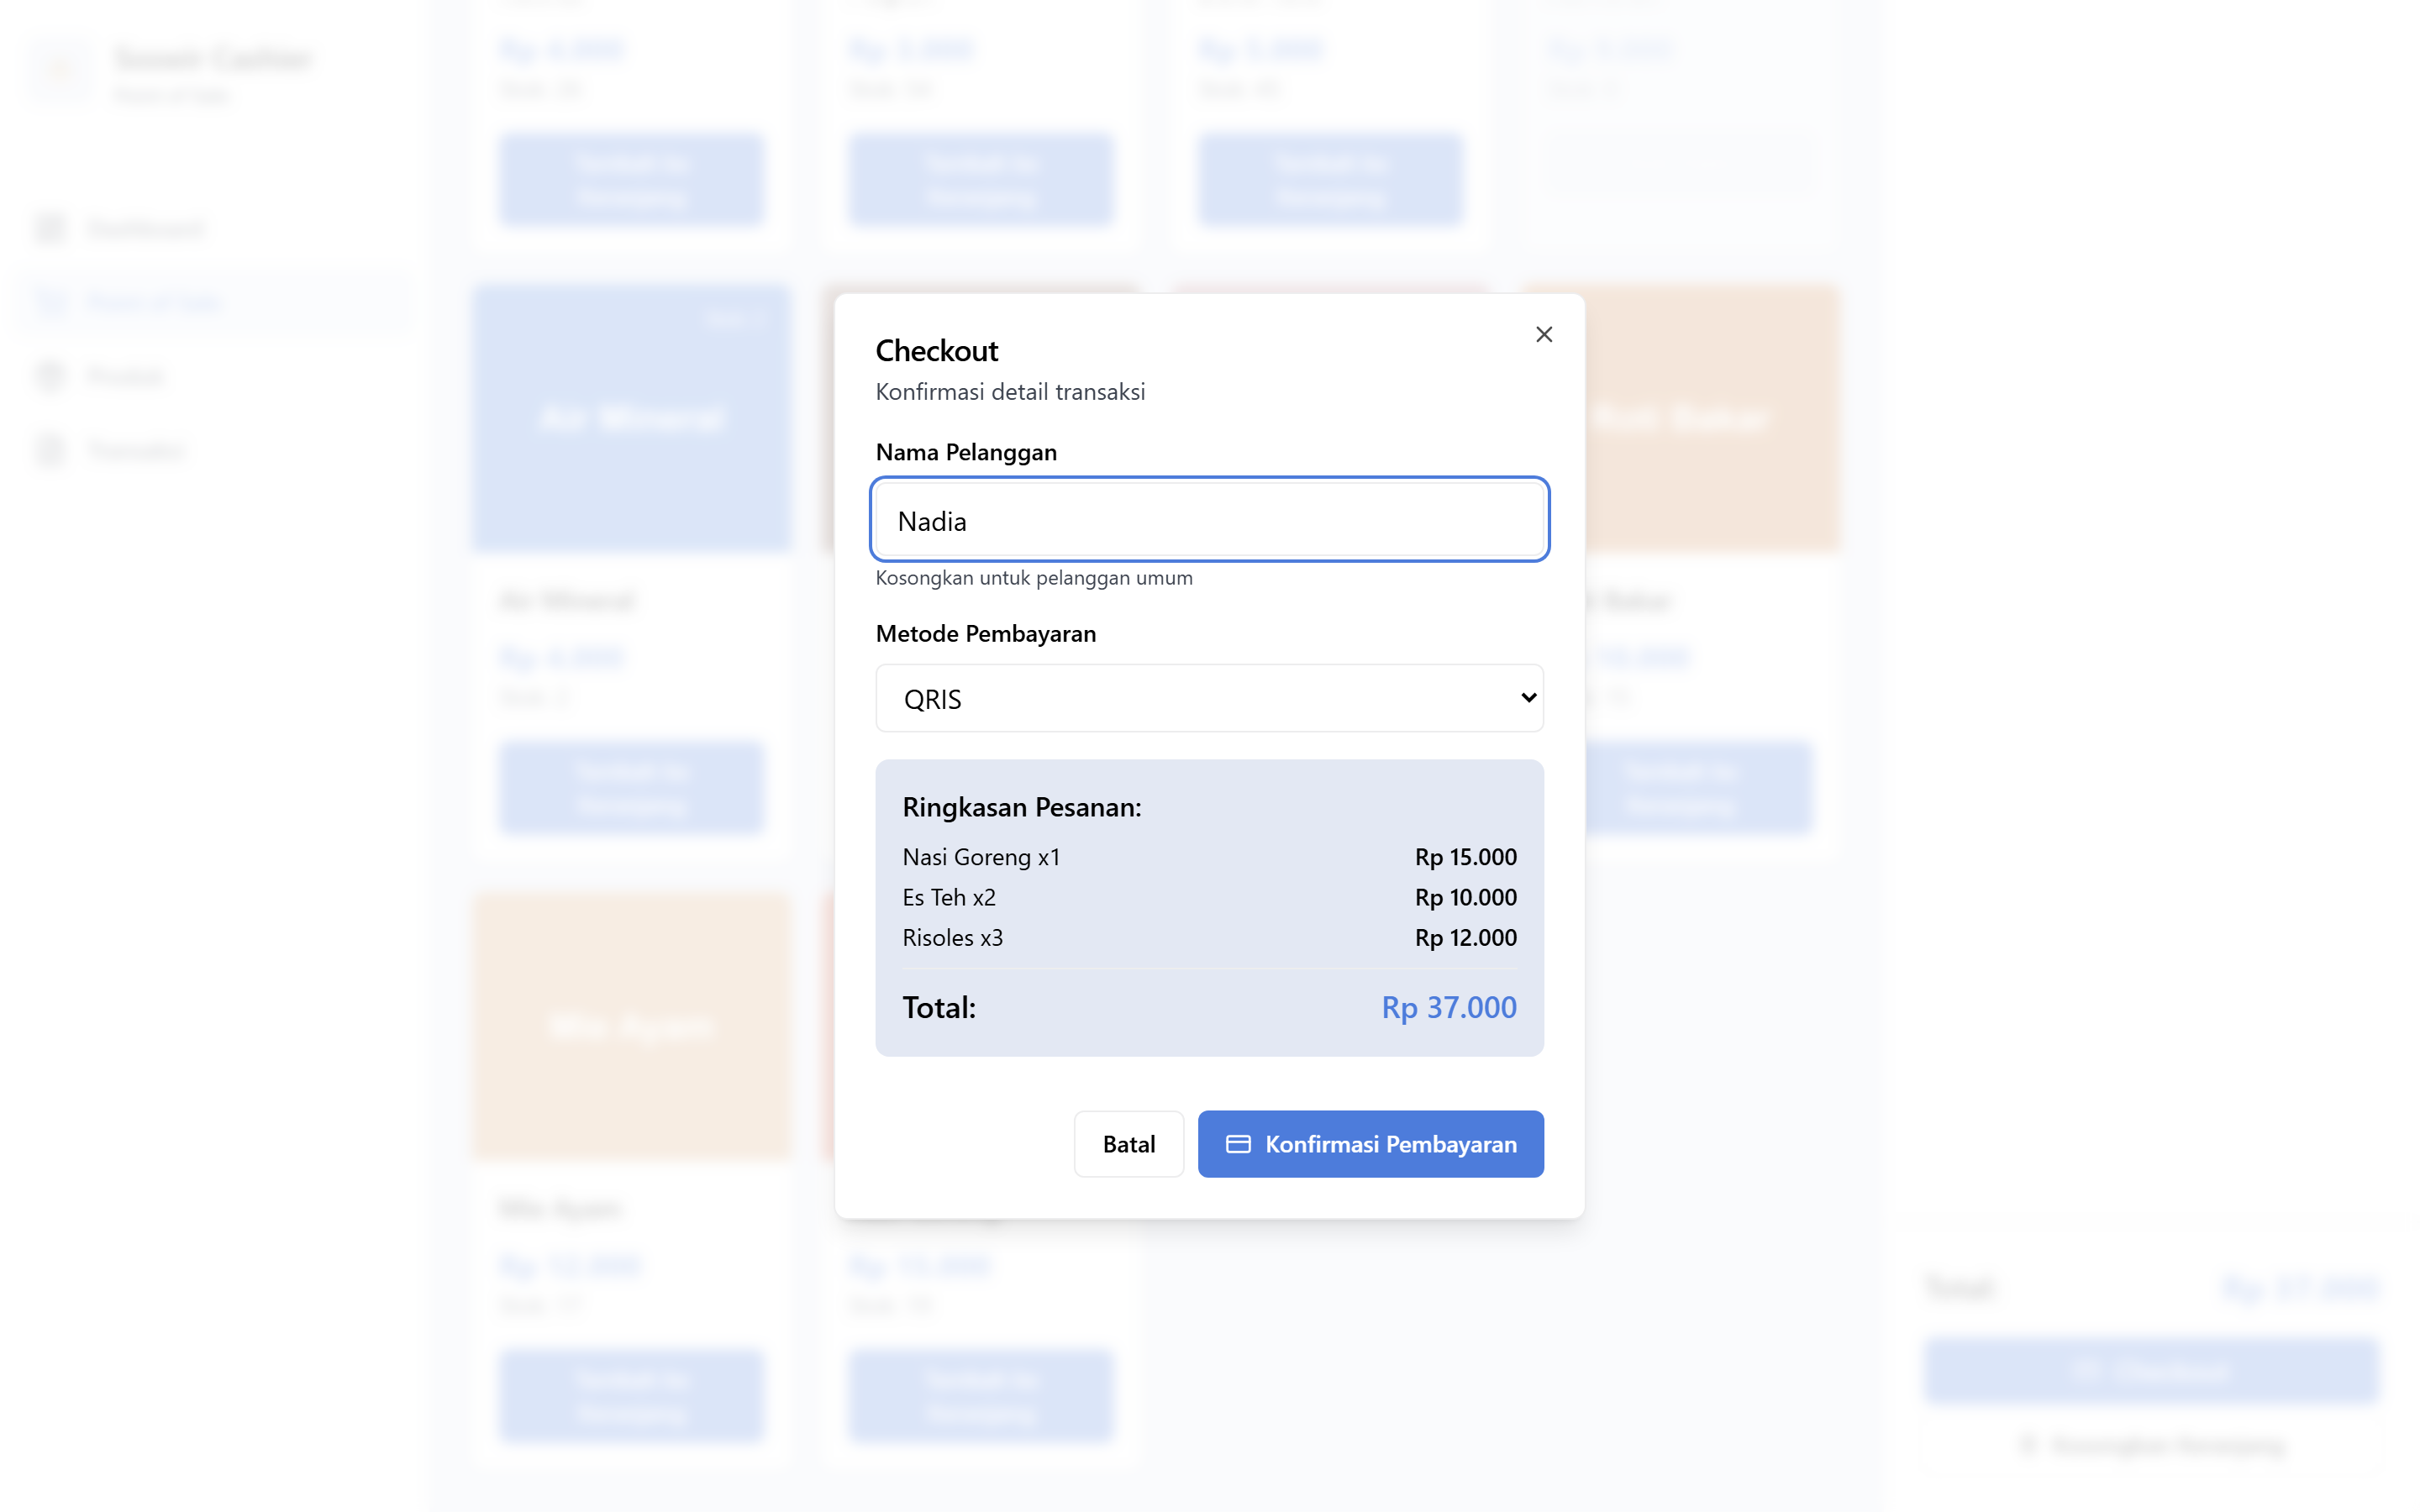
\includegraphics[width=0.99\linewidth,height=0.40\textheight,keepaspectratio,cfbox=garis 0.5pt 0pt]{img/07-pos-checkout.png}
\caption{Jendela \ui{Checkout} sebelum pembayaran dikonfirmasi.}
\end{figure}

\clearpage
\begin{enumerate}[resume]
  \item Setelah tersimpan, muncul pemberitahuan \ui{Berhasil!} dengan total penjualan di pojok kanan atas. Keranjang kosong lagi dan stok produk langsung berkurang.
\end{enumerate}

\begin{figure}[H]
\centering
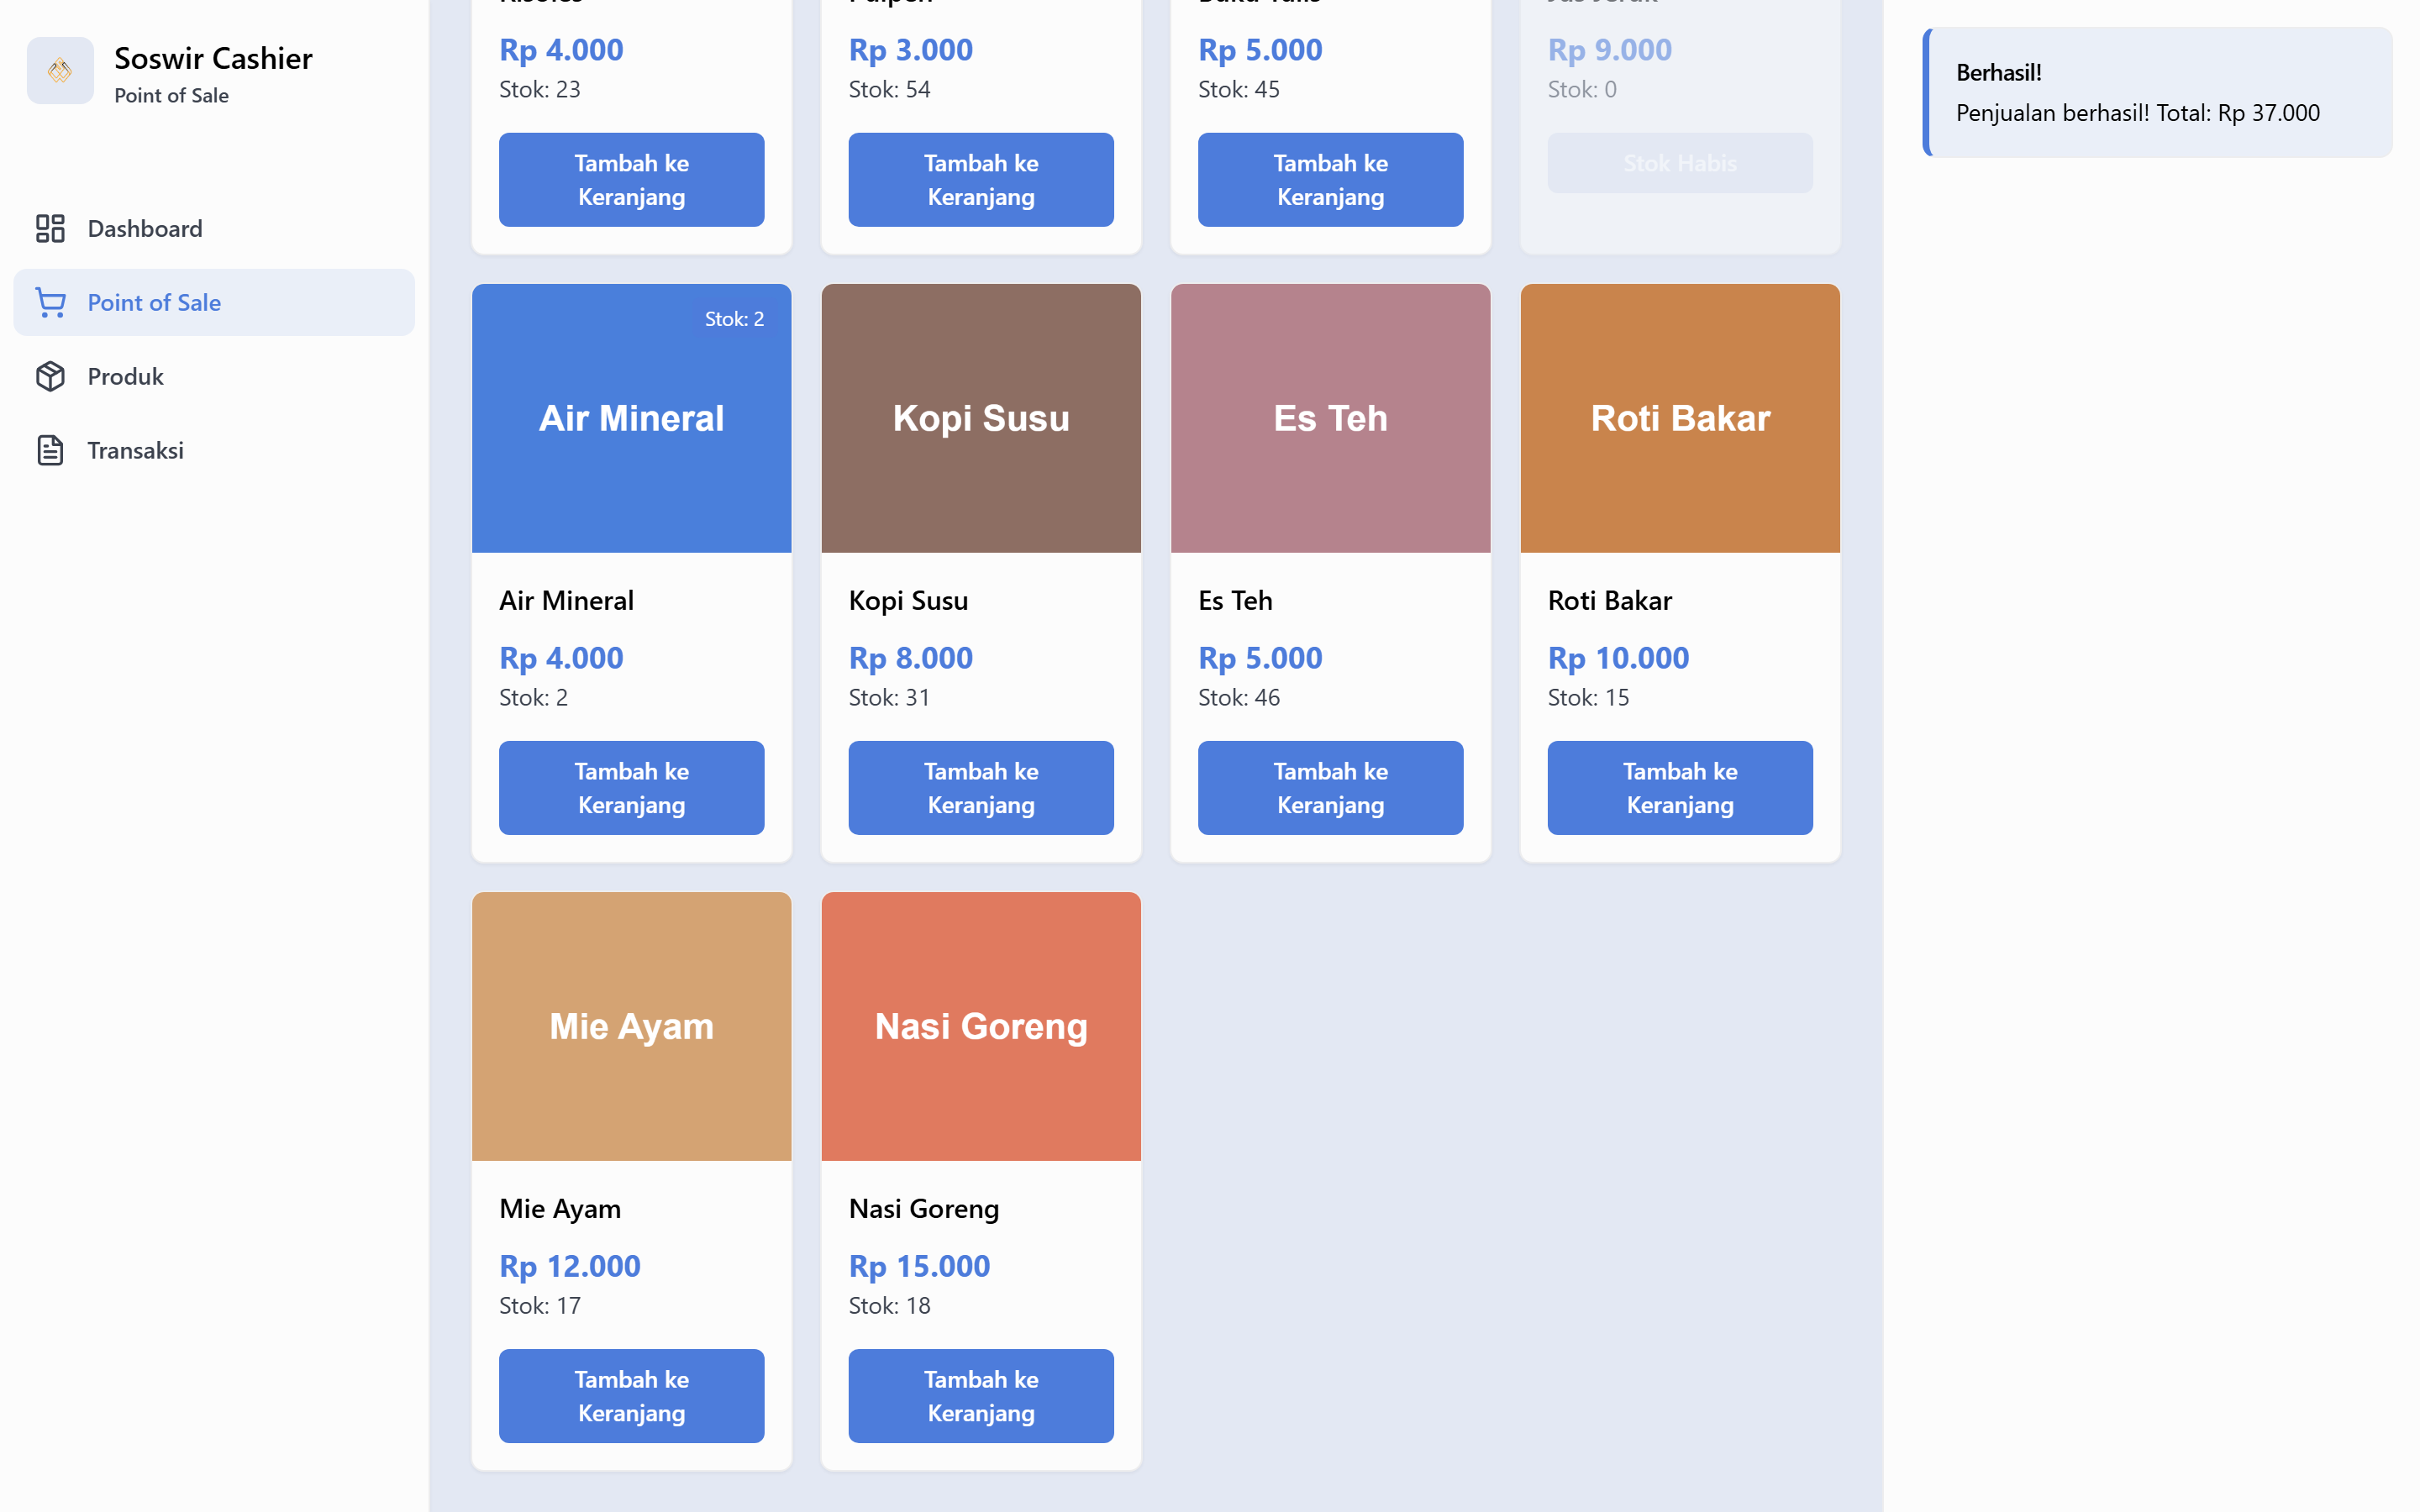
\includegraphics[width=0.99\linewidth,height=0.40\textheight,keepaspectratio,cfbox=garis 0.5pt 0pt]{img/08-pos-berhasil.png}
\caption{Pemberitahuan penjualan berhasil.}
\end{figure}

\begin{catatan}
Aplikasi tidak mencetak struk. Bukti transaksi ada di menu \ui{Transaksi}. Harga yang dipakai saat menyimpan selalu harga terbaru dari data produk, bukan harga yang sempat tampil di layar kasir. Jumlah barang harus bilangan bulat lebih dari nol.
\end{catatan}

\subsection{Stok habis atau tidak cukup}

Stok tidak bisa minus, jadi aplikasi menolak penjualan yang melebihi stok.

\begin{itemize}
  \item Produk dengan stok 0 tampil redup bertuliskan \ui{Stok Habis} dan tidak bisa dimasukkan ke keranjang.
  \item Produk yang stoknya tinggal sedikit memiliki penanda \ui{Stok: ...} di pojok gambar.
  \item Kalau jumlah di keranjang dinaikkan melebihi stok, muncul pesan \ui{Error!} ``Stok tidak mencukupi''.
  \item Kalau stok sempat berubah karena kasir lain menjual barang yang sama, penyimpanan ditolak dengan pesan berisi sisa stok yang tersedia. Kurangi jumlahnya lalu ulangi \ui{Checkout}.
  \item Barang titipan (PUBJ) hanya bisa dijual kalau hari ini sudah ada stok harian untuknya. Kalau belum, minta superadmin mencatat stok hariannya (lihat Bab~\ref{sec:stokharian}).
\end{itemize}

\begin{figure}[H]
\centering
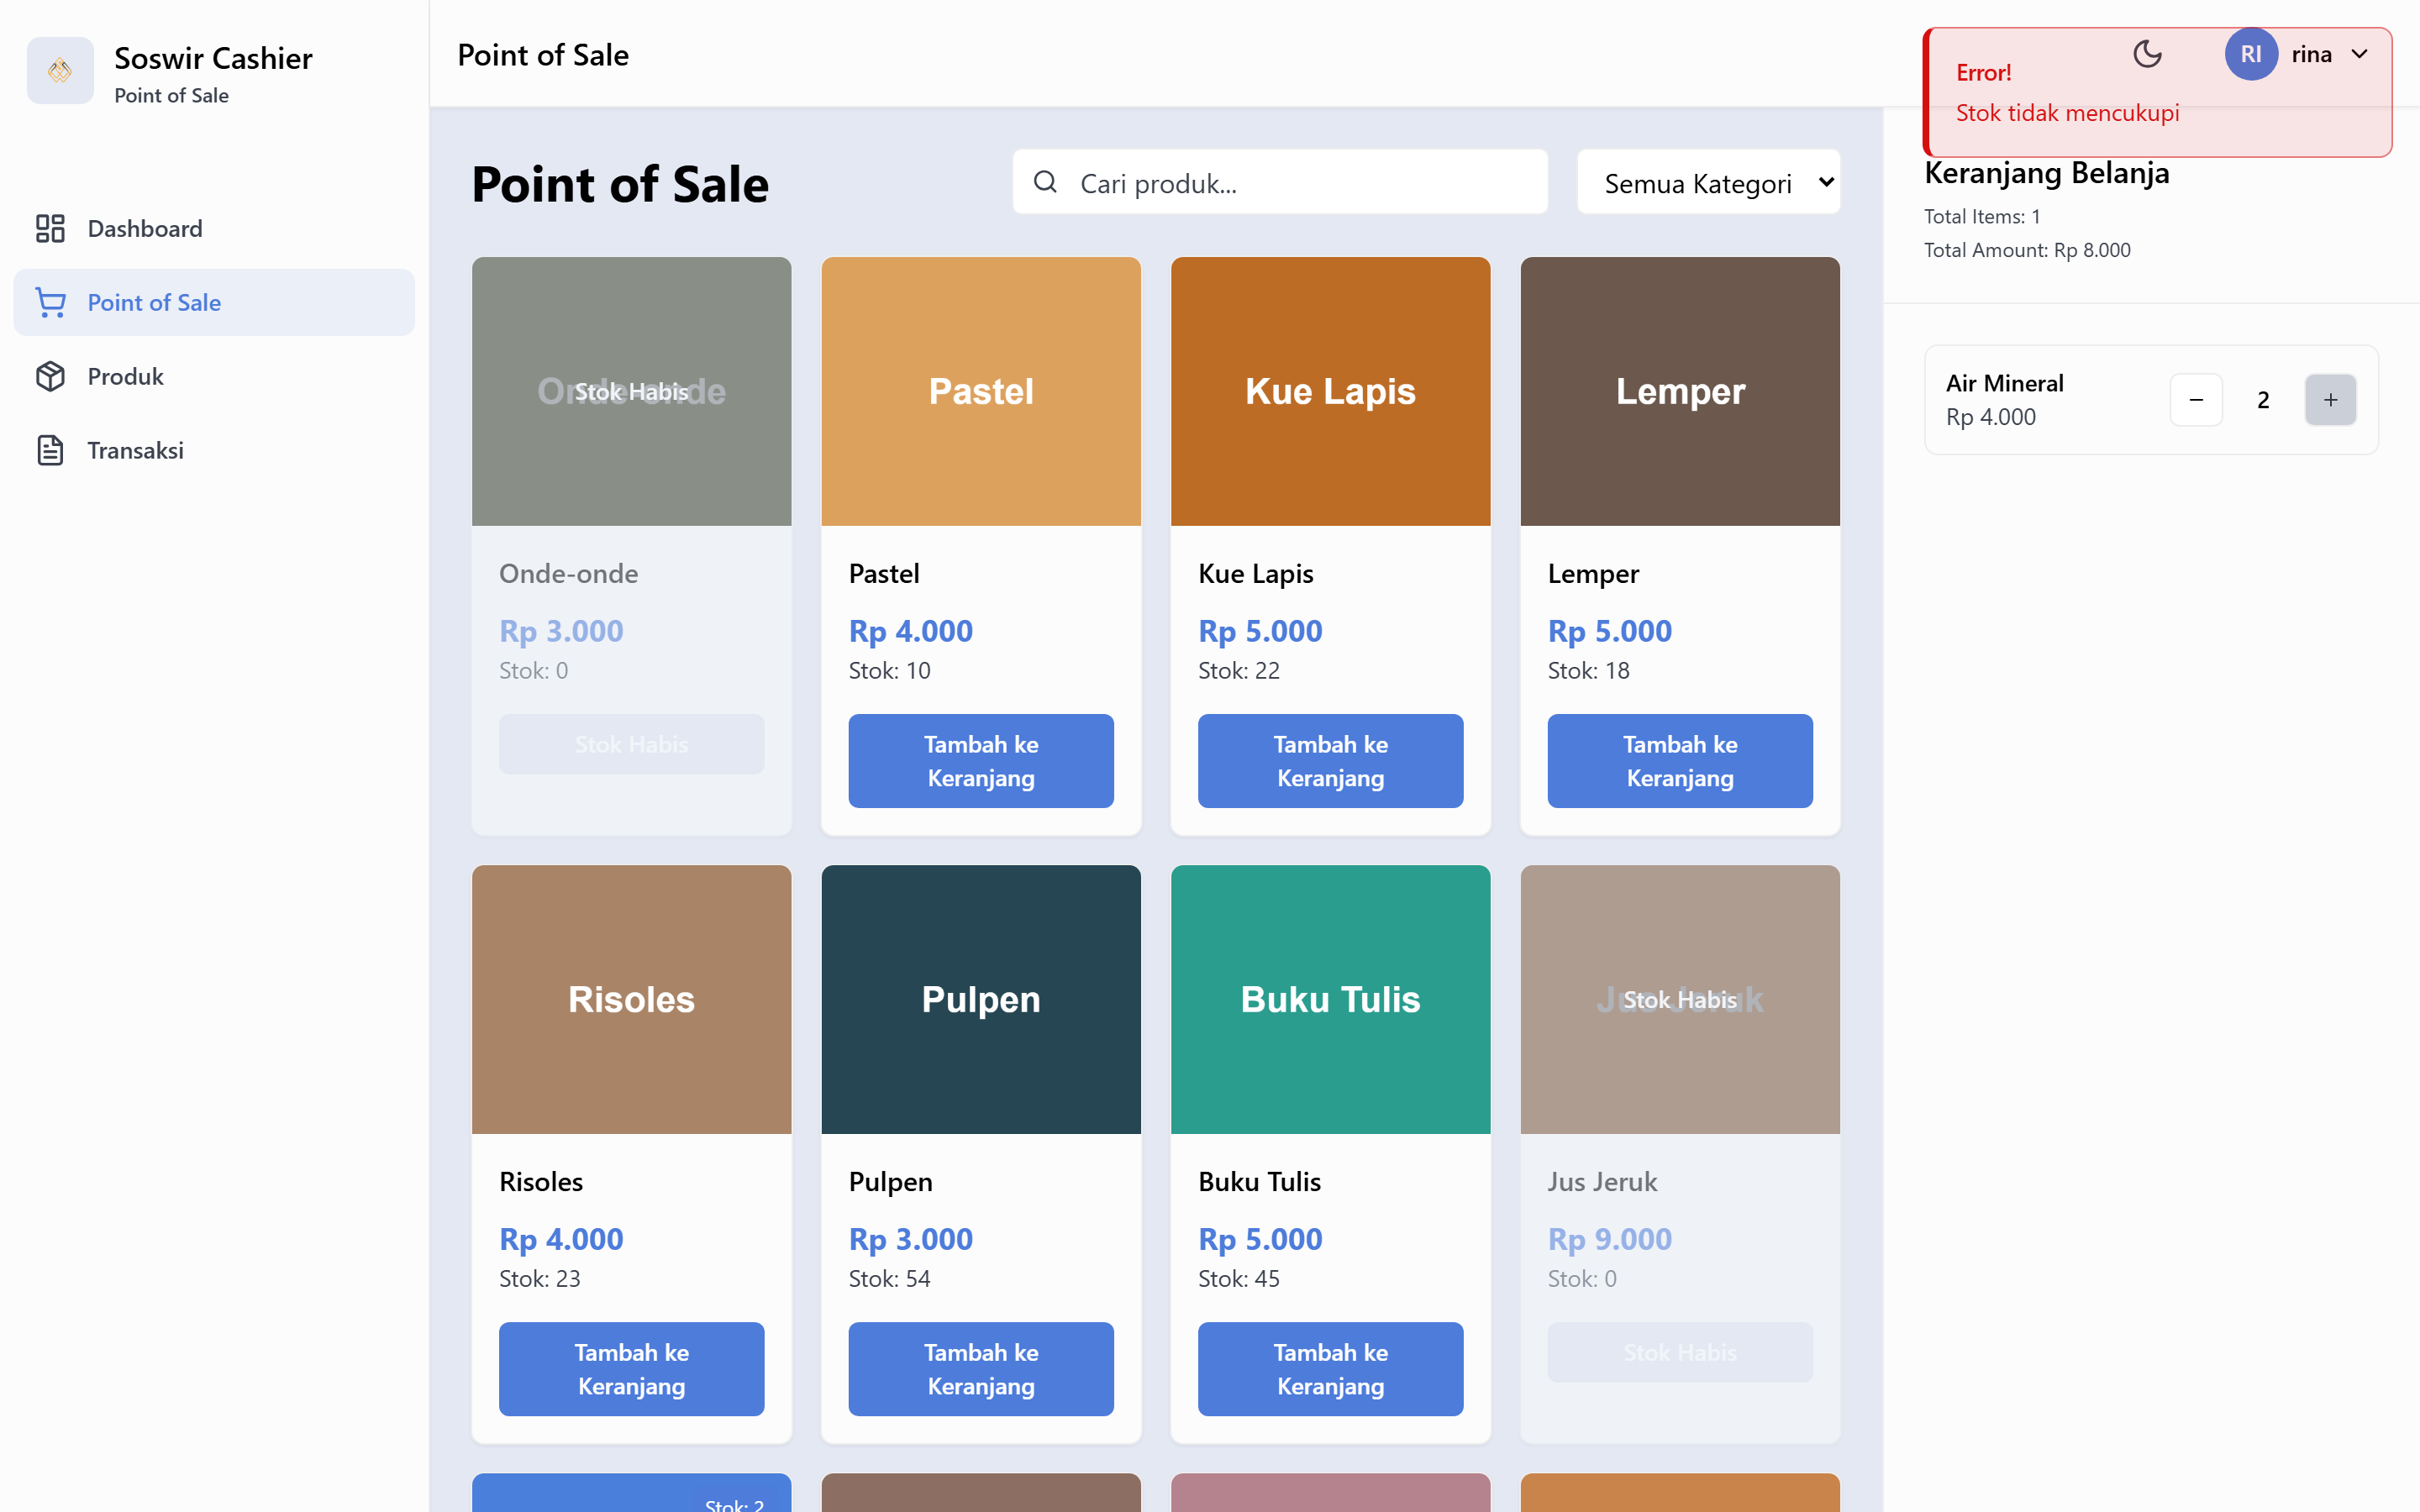
\includegraphics[width=0.99\linewidth,height=0.40\textheight,keepaspectratio,cfbox=garis 0.5pt 0pt]{img/09-pos-stok-tidak-cukup.png}
\caption{Pesan ``Stok tidak mencukupi'' saat jumlah Air Mineral melebihi stok. Onde-onde dan Jus Jeruk tampil \ui{Stok Habis}.}
\end{figure}

\subsection{Melihat daftar produk}

Menu \ui{Produk} menampilkan semua produk beserta harga, stok, dan status. Kasir hanya bisa melihat, tidak bisa mengubah.

\begin{enumerate}
  \item Tekan \ui{Produk} di menu kiri.
  \item Gunakan \ui{Pencarian}, \ui{Kategori}, dan \ui{Status Stok} (\ui{Semua}, \ui{Tersedia}, \ui{Habis}) untuk menyaring daftar. \ui{Reset Filter} mengembalikan tampilan semula.
  \item Atur urutan lewat \ui{Urutkan:}, atau tekan judul kolom.
\end{enumerate}

\begin{figure}[H]
\centering
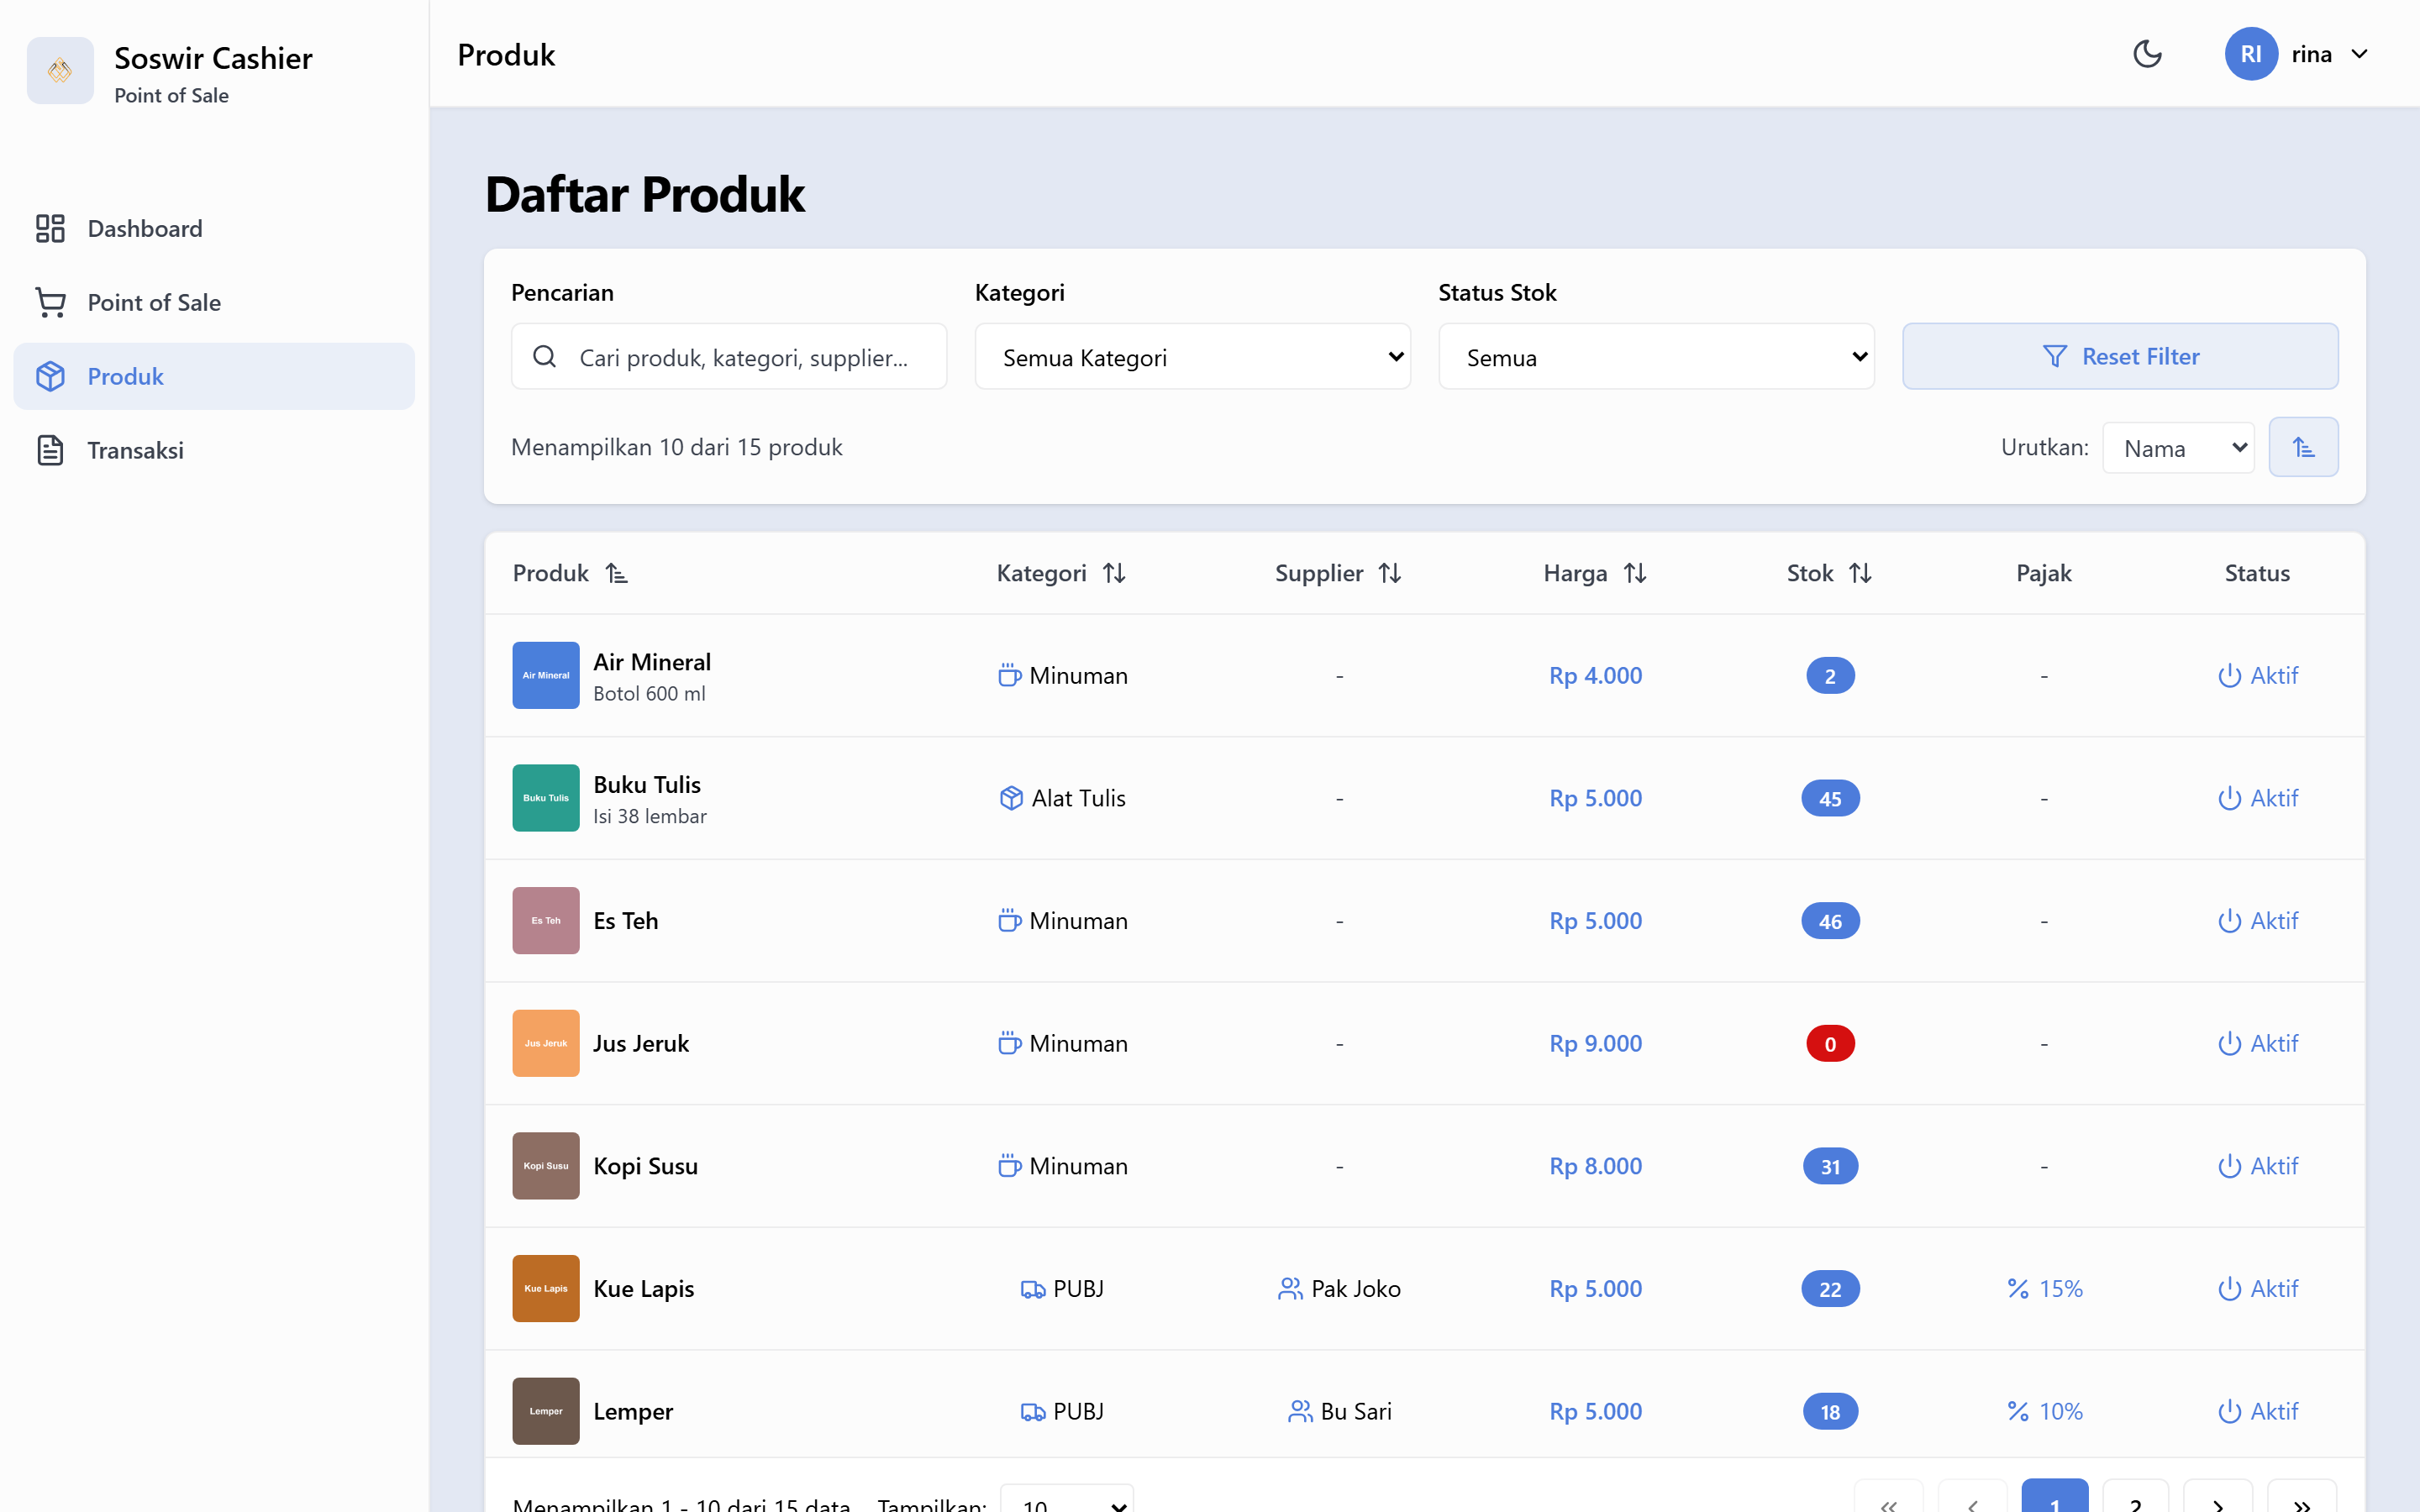
\includegraphics[width=0.99\linewidth,height=0.40\textheight,keepaspectratio,cfbox=garis 0.5pt 0pt]{img/10-kasir-produk.png}
\caption{\ui{Daftar Produk} untuk kasir.}
\end{figure}

\subsection{Riwayat transaksi kasir}

Menu \ui{Transaksi} menampilkan \ui{Log Transaksi} milik kasir yang sedang masuk. Satu baris adalah satu produk dalam satu transaksi.

\begin{enumerate}
  \item Tekan \ui{Transaksi} di menu kiri.
  \item Cari lewat kotak \ui{Cari transaksi...}, atau isi dua kotak tanggal untuk membatasi rentang tanggal. \ui{Reset} menghapus saringan.
  \item Tekan \ui{Ekspor ke CSV} untuk mengunduh daftar yang sedang tampil.
\end{enumerate}

\begin{figure}[H]
\centering
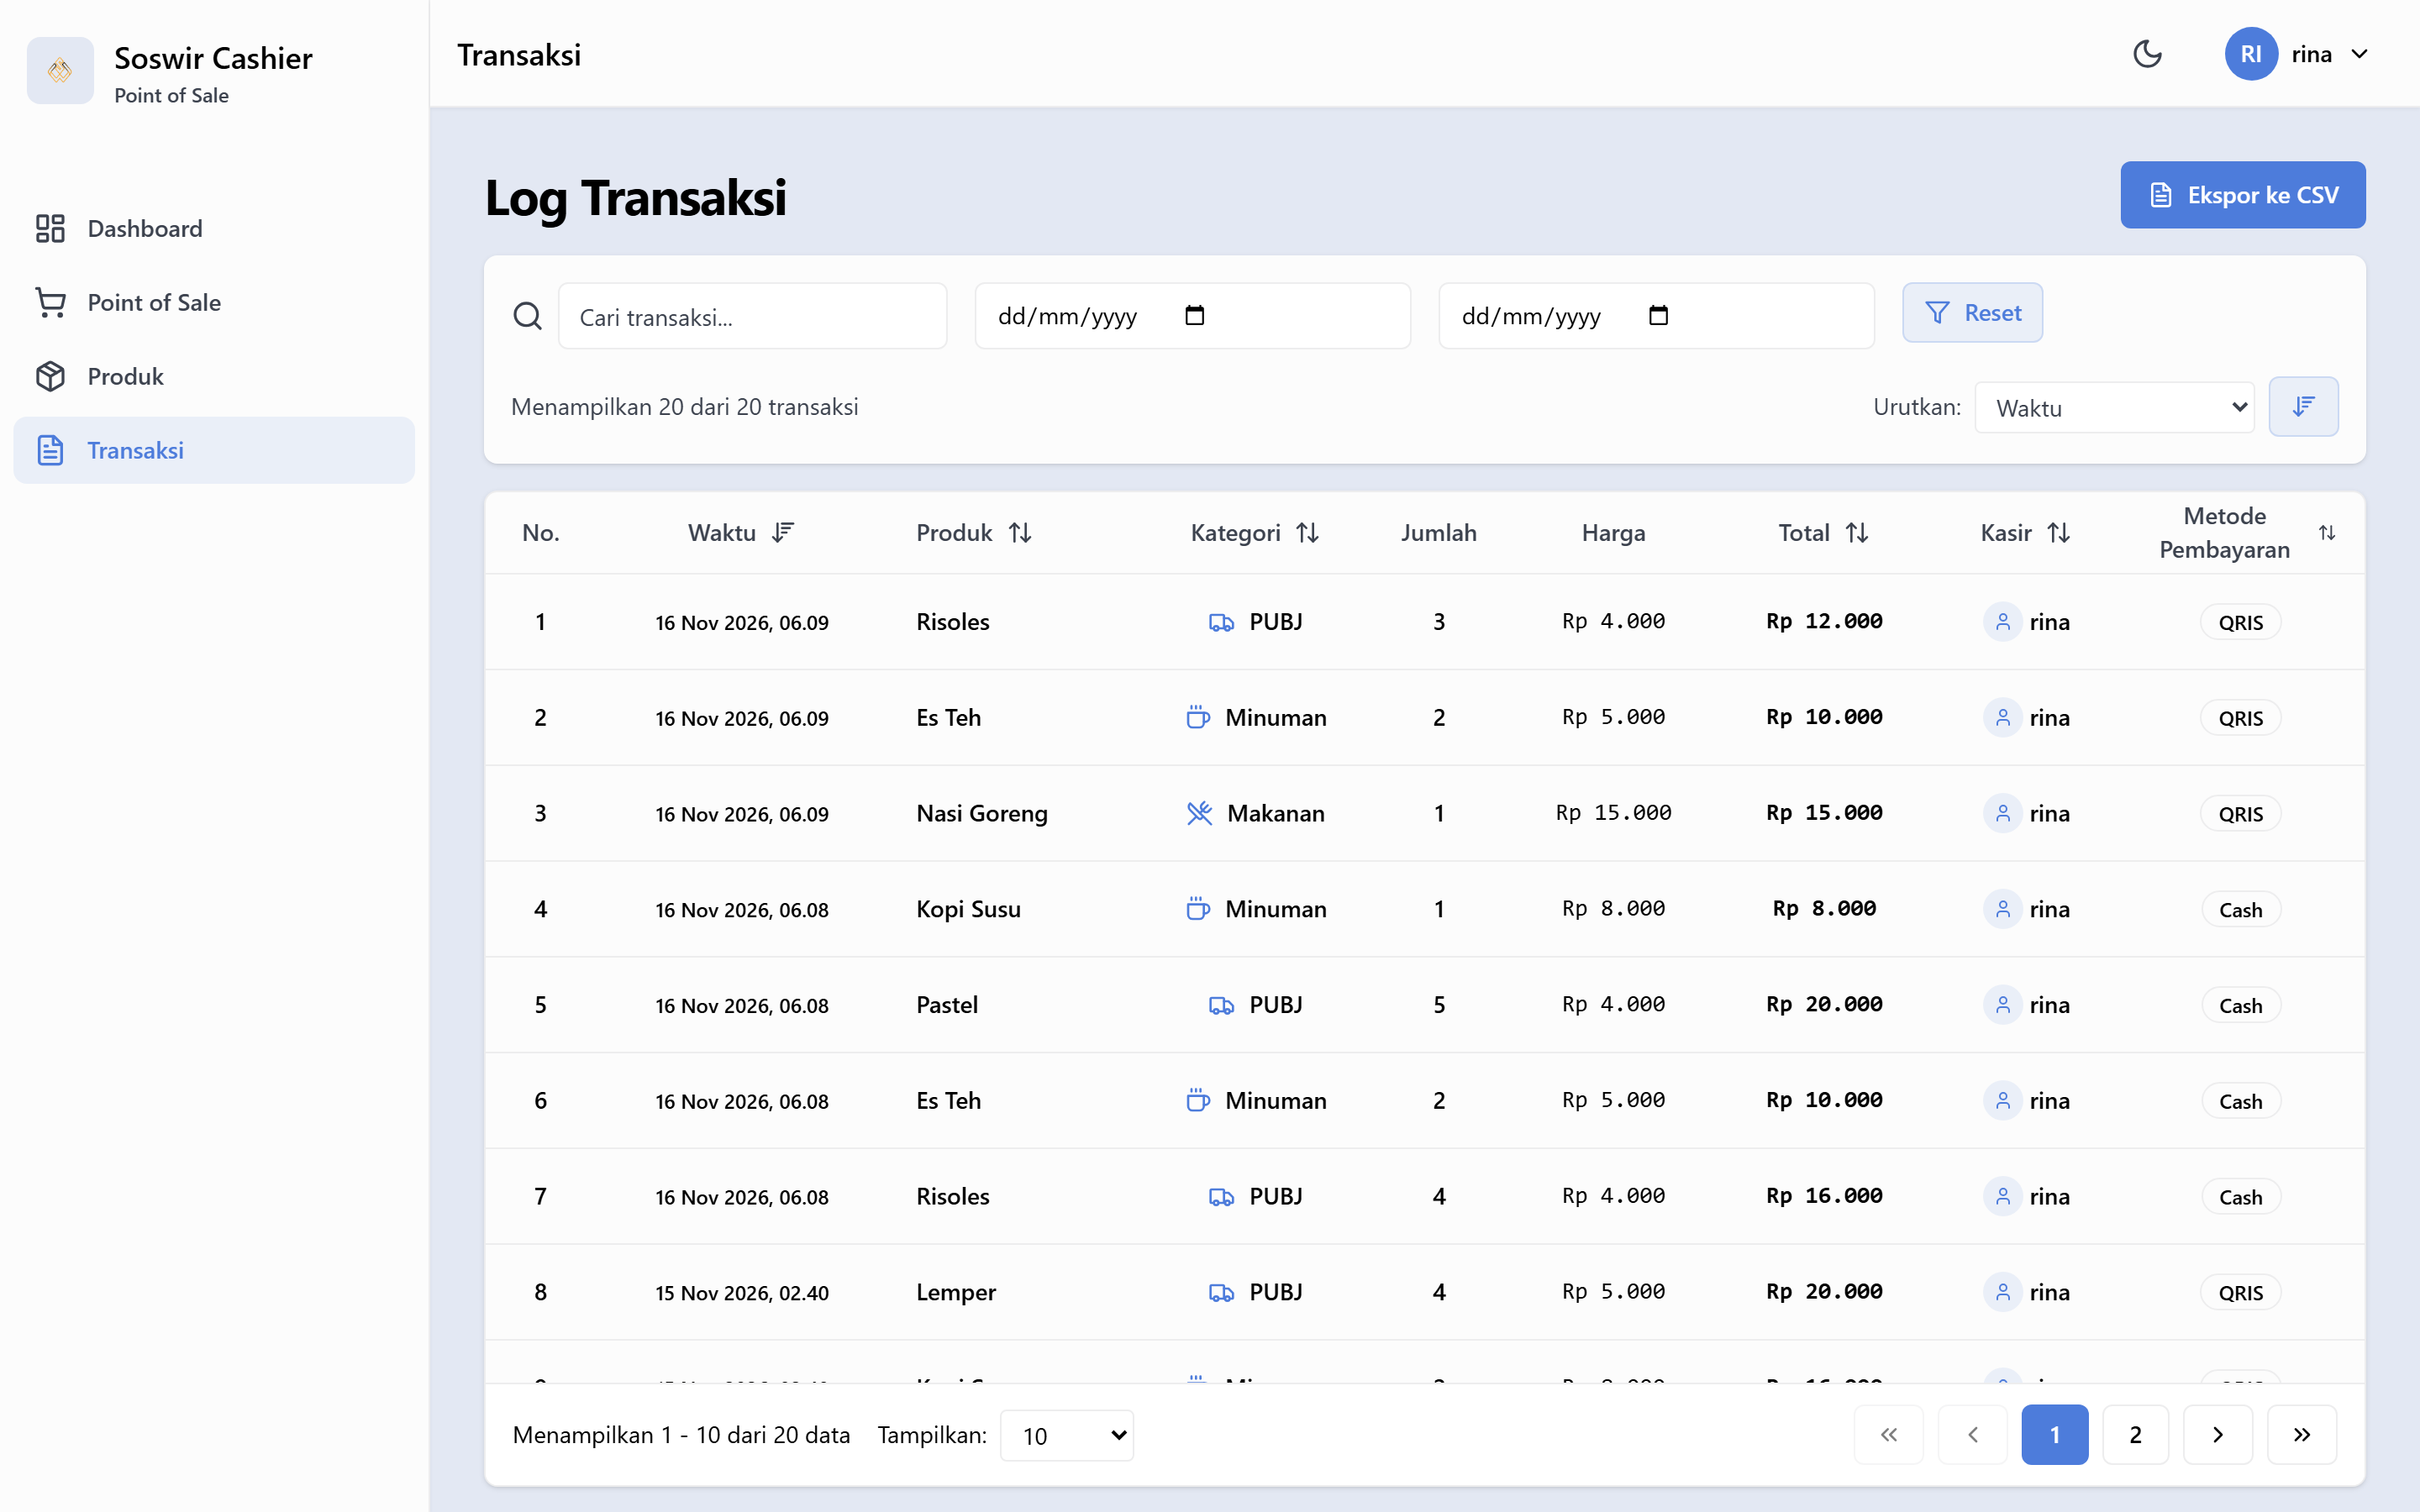
\includegraphics[width=0.99\linewidth,height=0.40\textheight,keepaspectratio,cfbox=garis 0.5pt 0pt]{img/11-kasir-transaksi.png}
\caption{\ui{Log Transaksi} kasir.}
\end{figure}

% ---------------------------------------------------------------
\section{Dashboard Superadmin}

Halaman \ui{Dashboard} terbuka setelah superadmin masuk. Bagian atas berisi delapan kartu angka.

\begin{figure}[H]
\centering
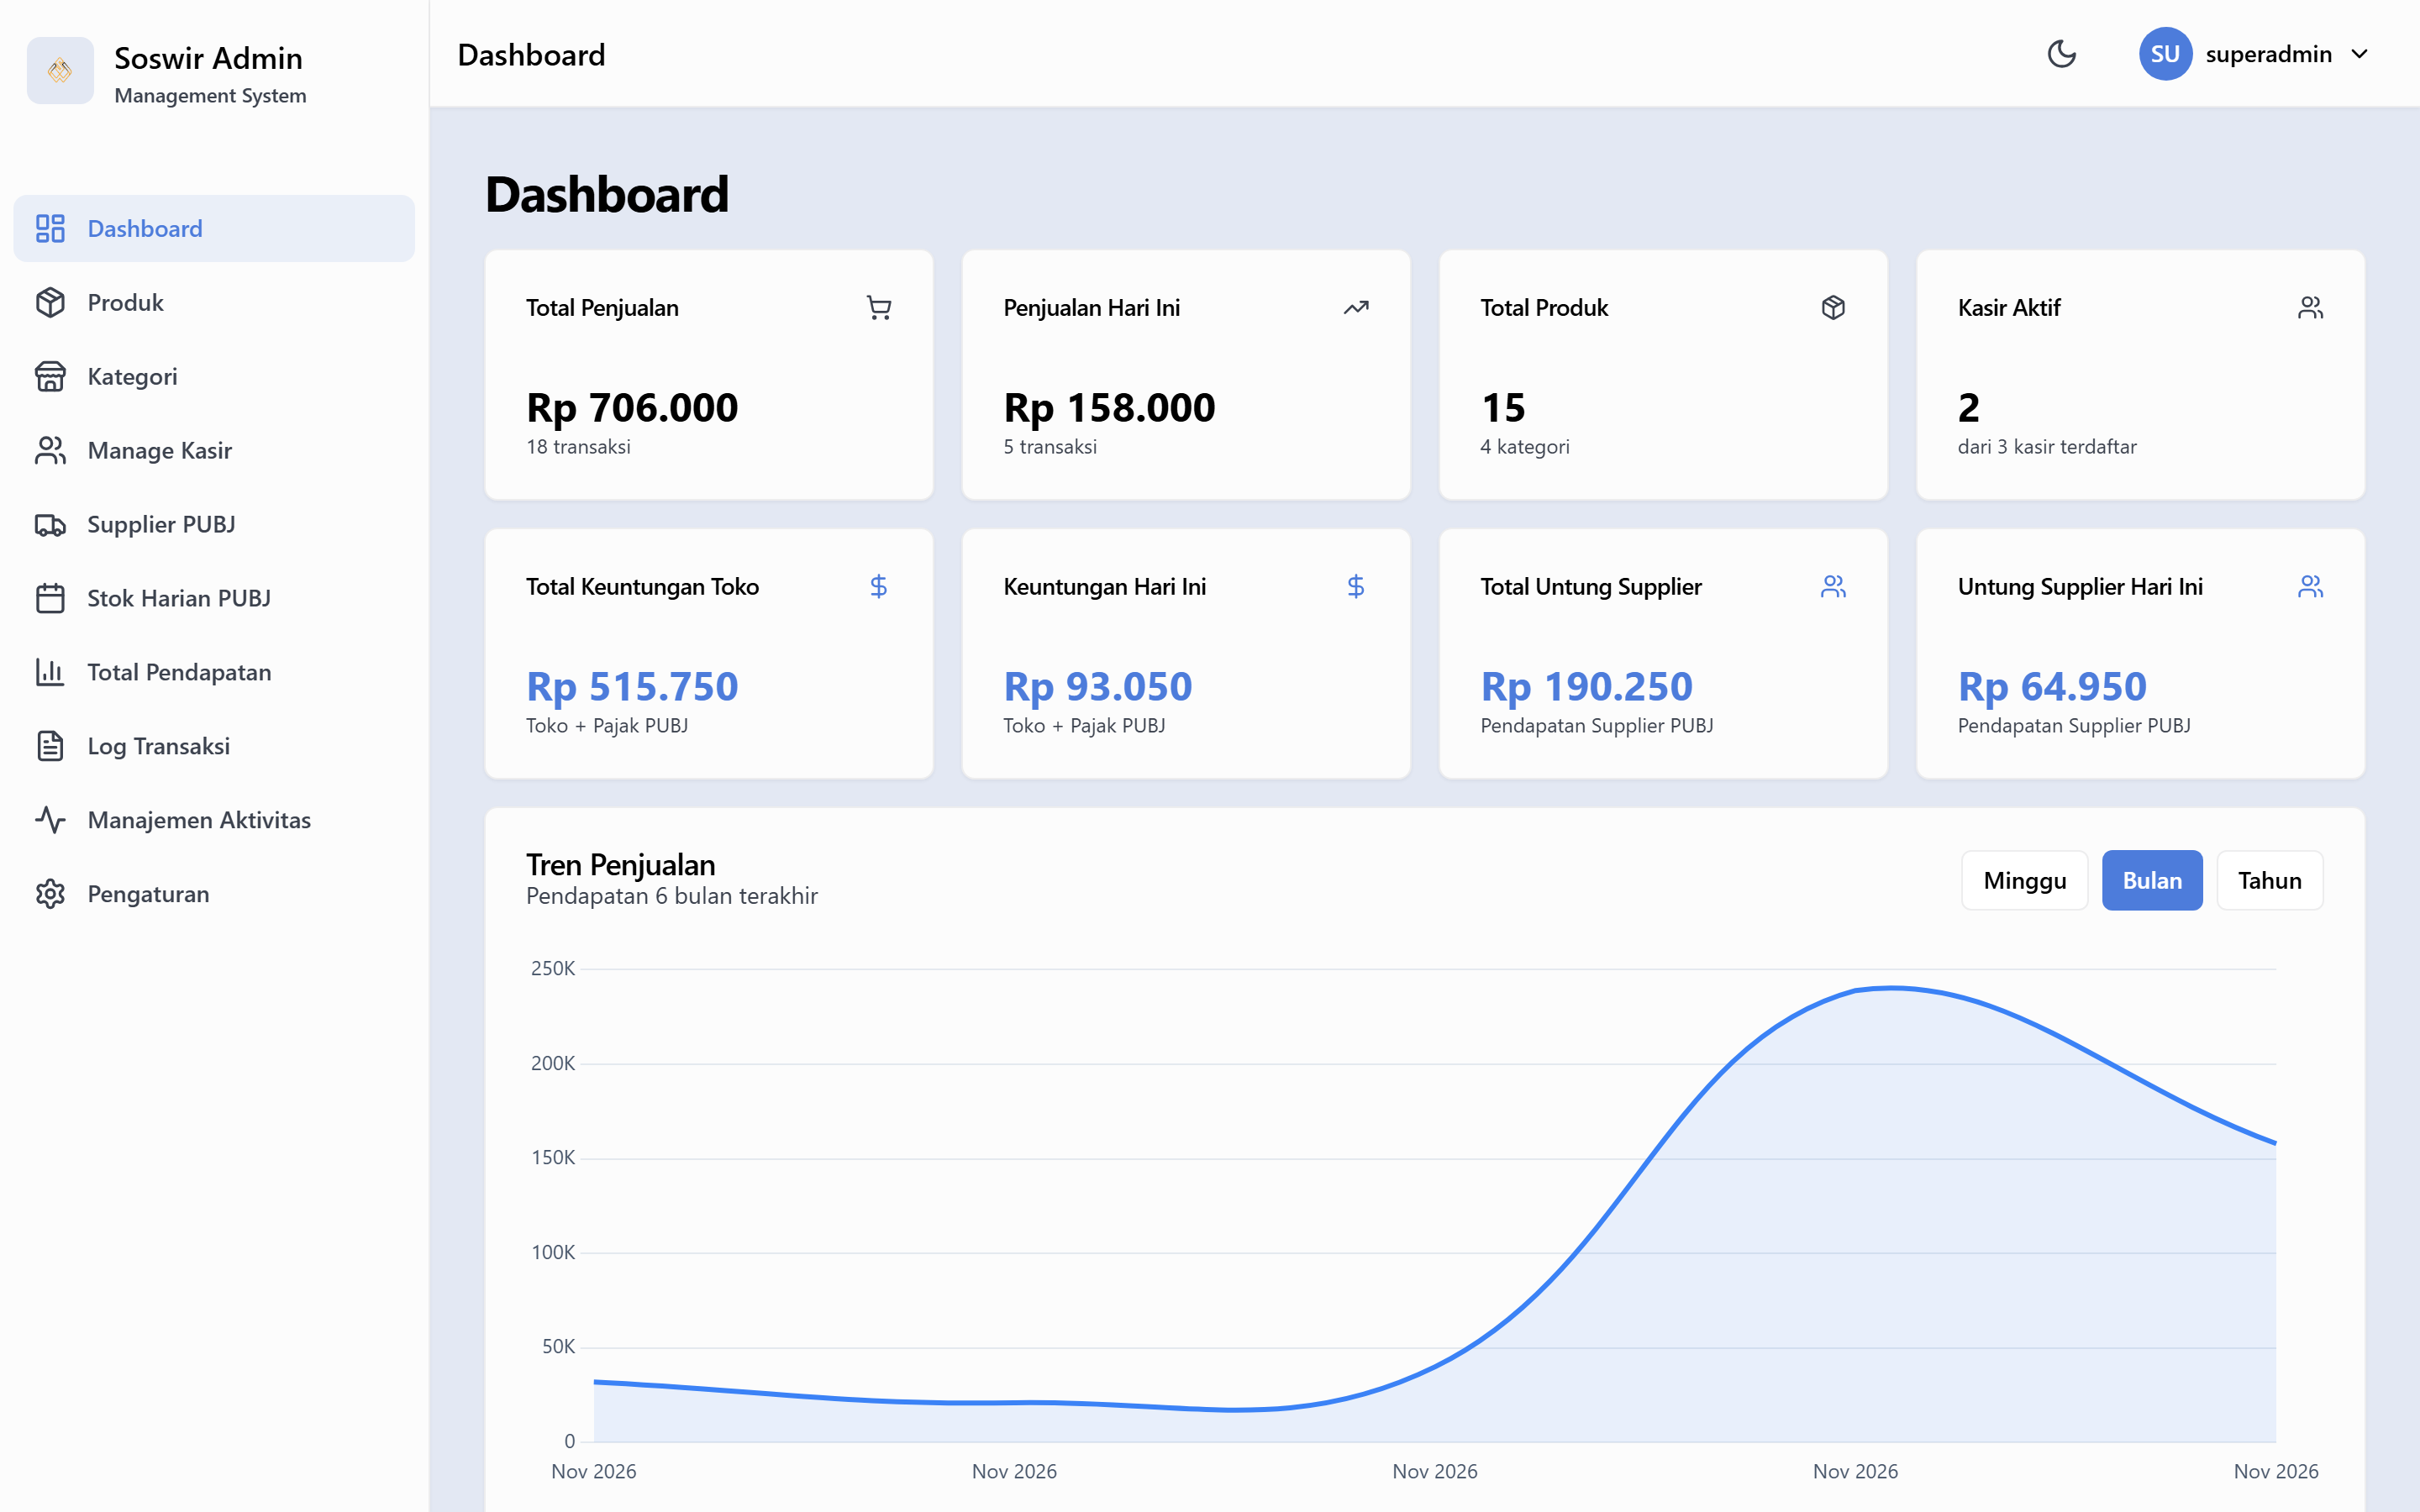
\includegraphics[width=0.99\linewidth,height=0.40\textheight,keepaspectratio,cfbox=garis 0.5pt 0pt]{img/13-admin-dashboard.png}
\caption{Kartu angka dan grafik \ui{Tren Penjualan}.}
\end{figure}

\begin{center}
\small
\begin{tabular}{@{}>{\raggedright\arraybackslash}p{4.4cm}>{\raggedright\arraybackslash}p{11.1cm}@{}}
\toprule
\textbf{Kartu} & \textbf{Arti} \\
\midrule
Total Penjualan & Seluruh uang penjualan sejak awal, termasuk barang titipan. \\
Penjualan Hari Ini & Uang penjualan hari ini dan jumlah transaksinya. \\
Total Produk & Jumlah produk dan jumlah kategori. \\
Kasir Aktif & Kasir yang sedang aktif dibanding semua kasir terdaftar. \\
Total Keuntungan Toko & Bagian toko: 100\% penjualan produk toko ditambah fee toko dari barang titipan PUBJ. \\
Keuntungan Hari Ini & Sama seperti di atas, khusus hari ini. \\
Total Untung Supplier & Bagian supplier dari penjualan barang titipan, yaitu harga jual dikurangi fee toko. \\
Untung Supplier Hari Ini & Sama seperti di atas, khusus hari ini. \\
\bottomrule
\end{tabular}
\end{center}

Contoh: Risoles titipan dijual Rp 4.000 dengan fee toko 10\%. Setiap Risoles terjual, toko mendapat Rp 400 dan supplier Rp 3.600. Nasi Goreng adalah produk toko, jadi seluruh Rp 15.000 masuk ke keuntungan toko.

Grafik \ui{Tren Penjualan} bisa diganti tampilannya dengan tombol \ui{Minggu}, \ui{Bulan}, atau \ui{Tahun}.

\clearpage
Gulir ke bawah untuk melihat ringkasan lain:

\begin{itemize}
  \item \ui{Performa Kategori \& Pajak PUBJ}: penjualan per kategori 30 hari terakhir. Kategori PUBJ menampilkan rincian \ui{Pajak} (fee toko) dan \ui{Supplier}.
  \item \ui{Produk Terlaris}: produk paling laku 30 hari terakhir. Barang titipan menampilkan fee toko di bawah angkanya.
  \item \ui{Transaksi Terbaru} dan \ui{Aktivitas Terkini}: transaksi dan aktivitas pengguna paling baru. Tombol \ui{Lihat Semua Aktivitas} membuka daftar lengkapnya.
\end{itemize}

\begin{figure}[H]
\centering
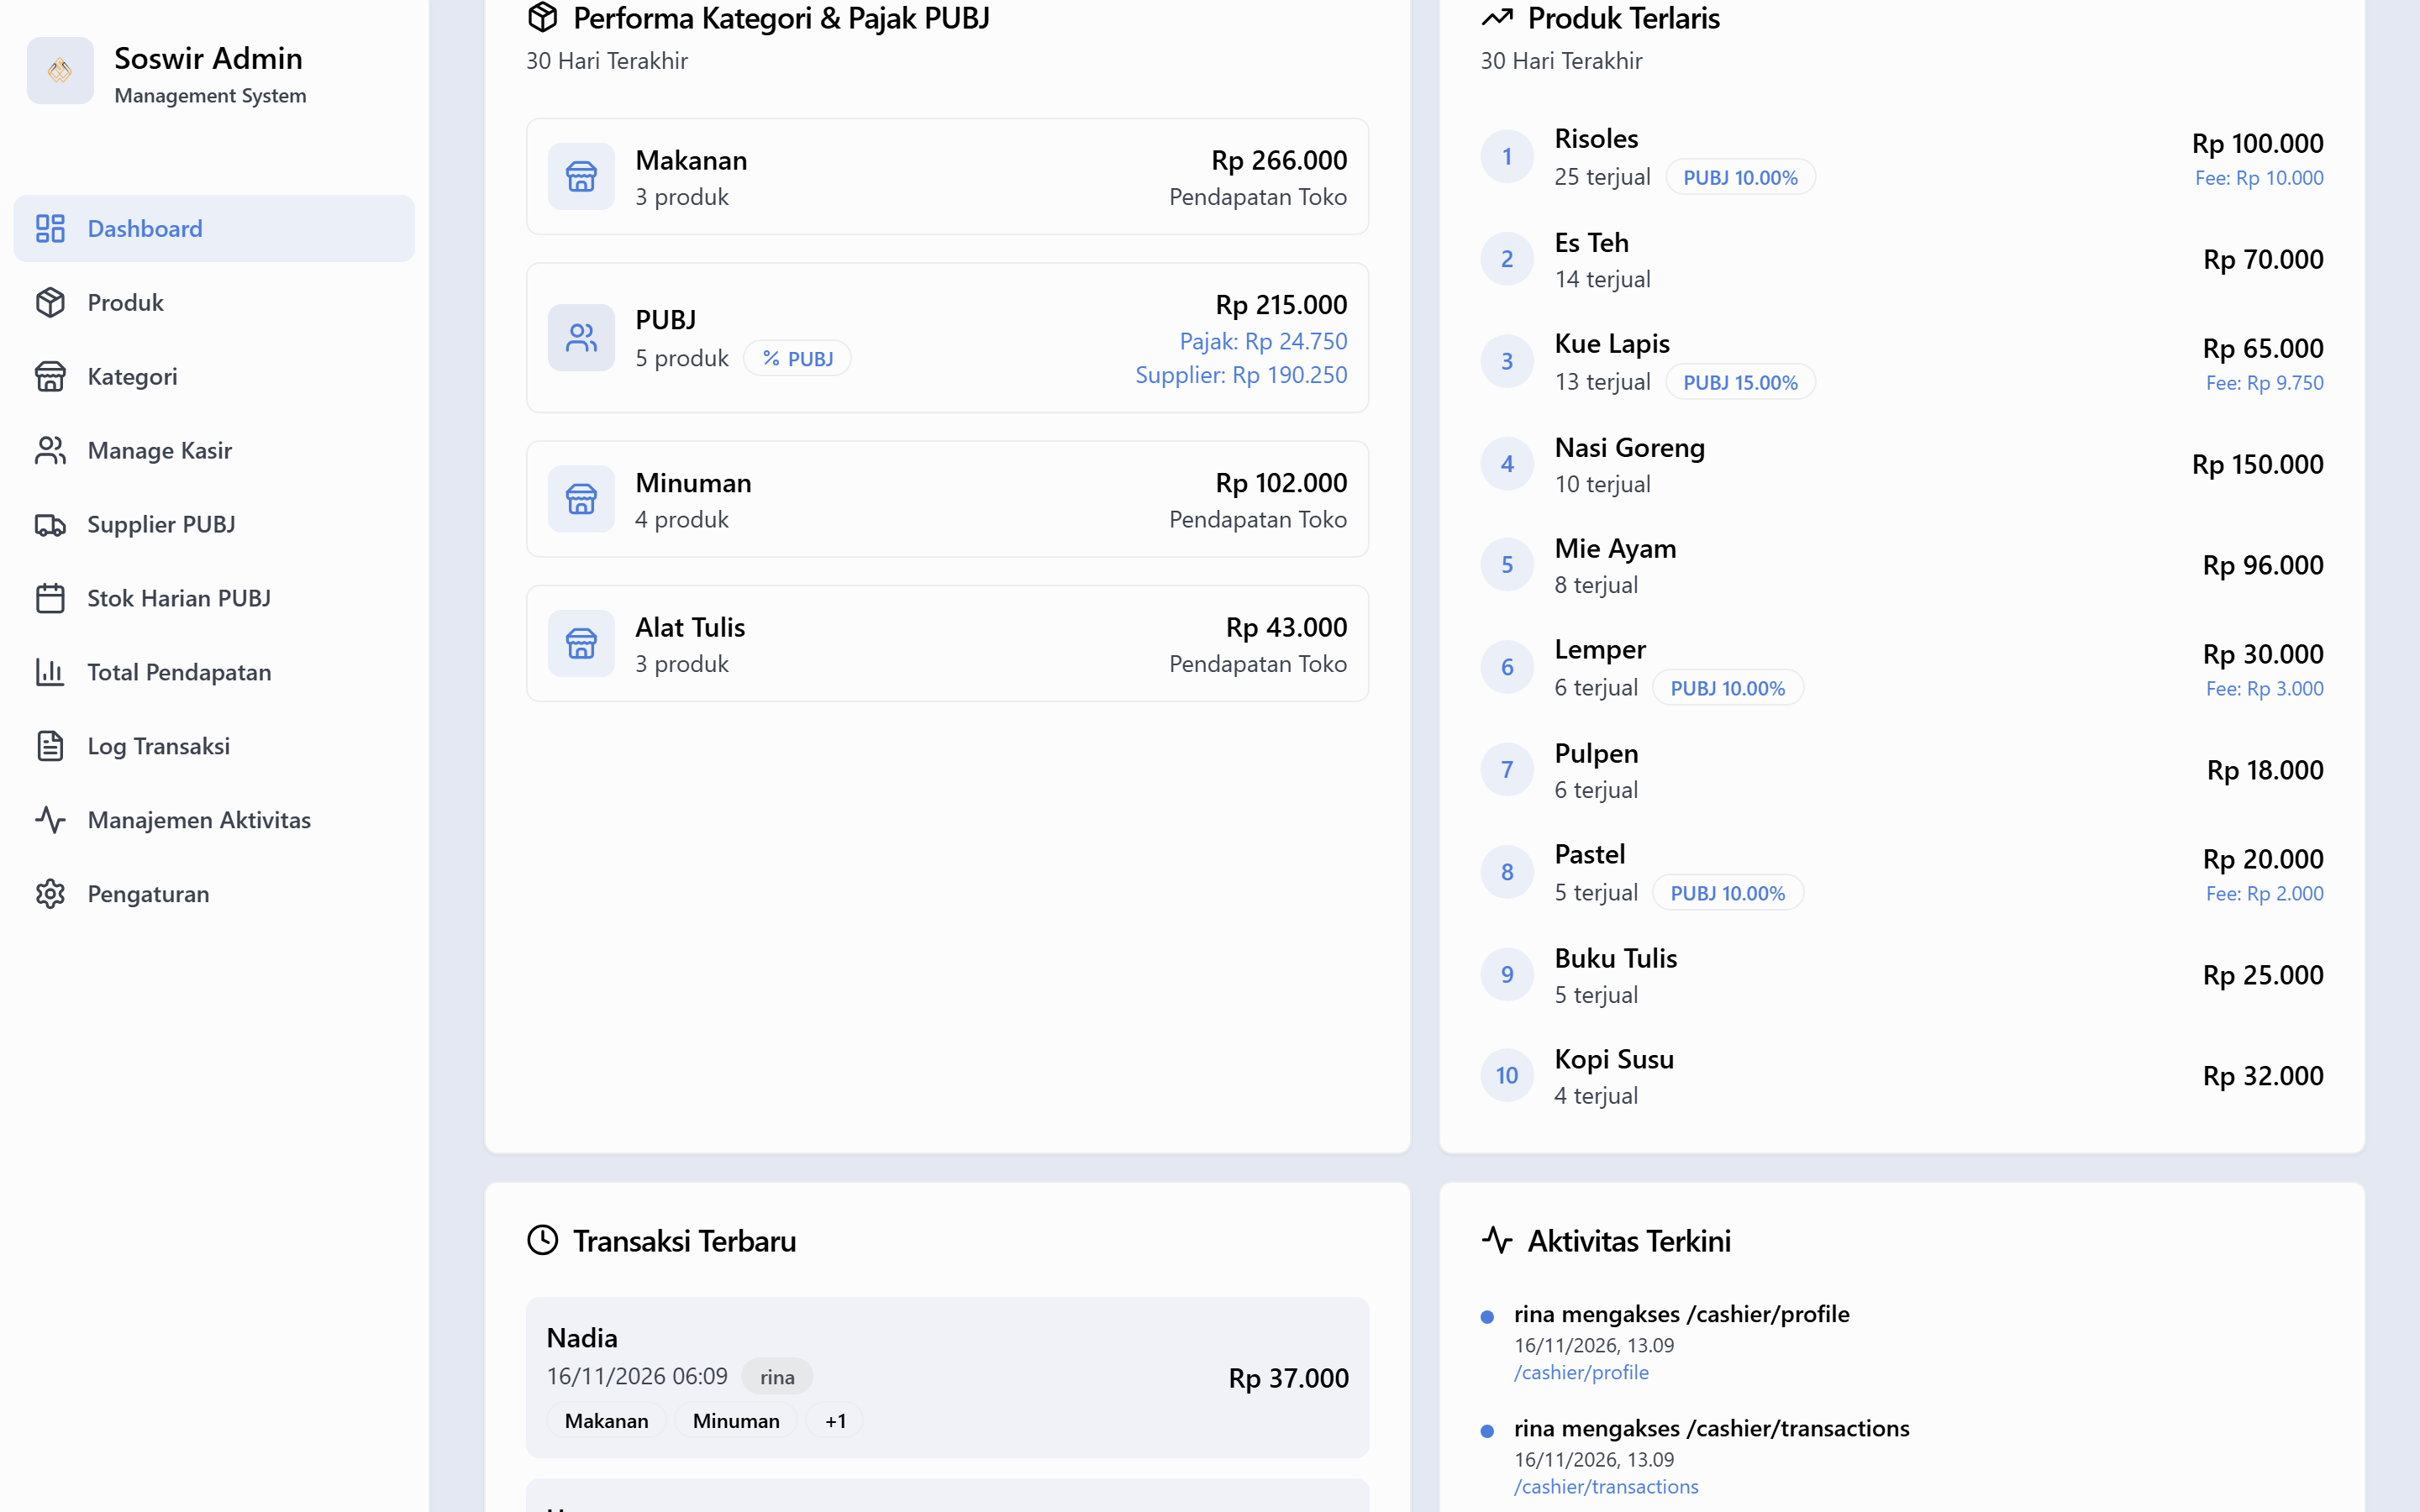
\includegraphics[width=0.99\linewidth,height=0.40\textheight,keepaspectratio,cfbox=garis 0.5pt 0pt]{img/14-admin-dashboard-ringkasan.png}
\caption{Ringkasan kategori, produk terlaris, transaksi, dan aktivitas.}
\end{figure}

% ---------------------------------------------------------------
\section{Produk}

Menu \ui{Produk} membuka halaman \ui{Manajemen Produk}. Di sini superadmin menambah produk, mengubah harga, menambah stok, dan menonaktifkan produk.

\begin{figure}[H]
\centering
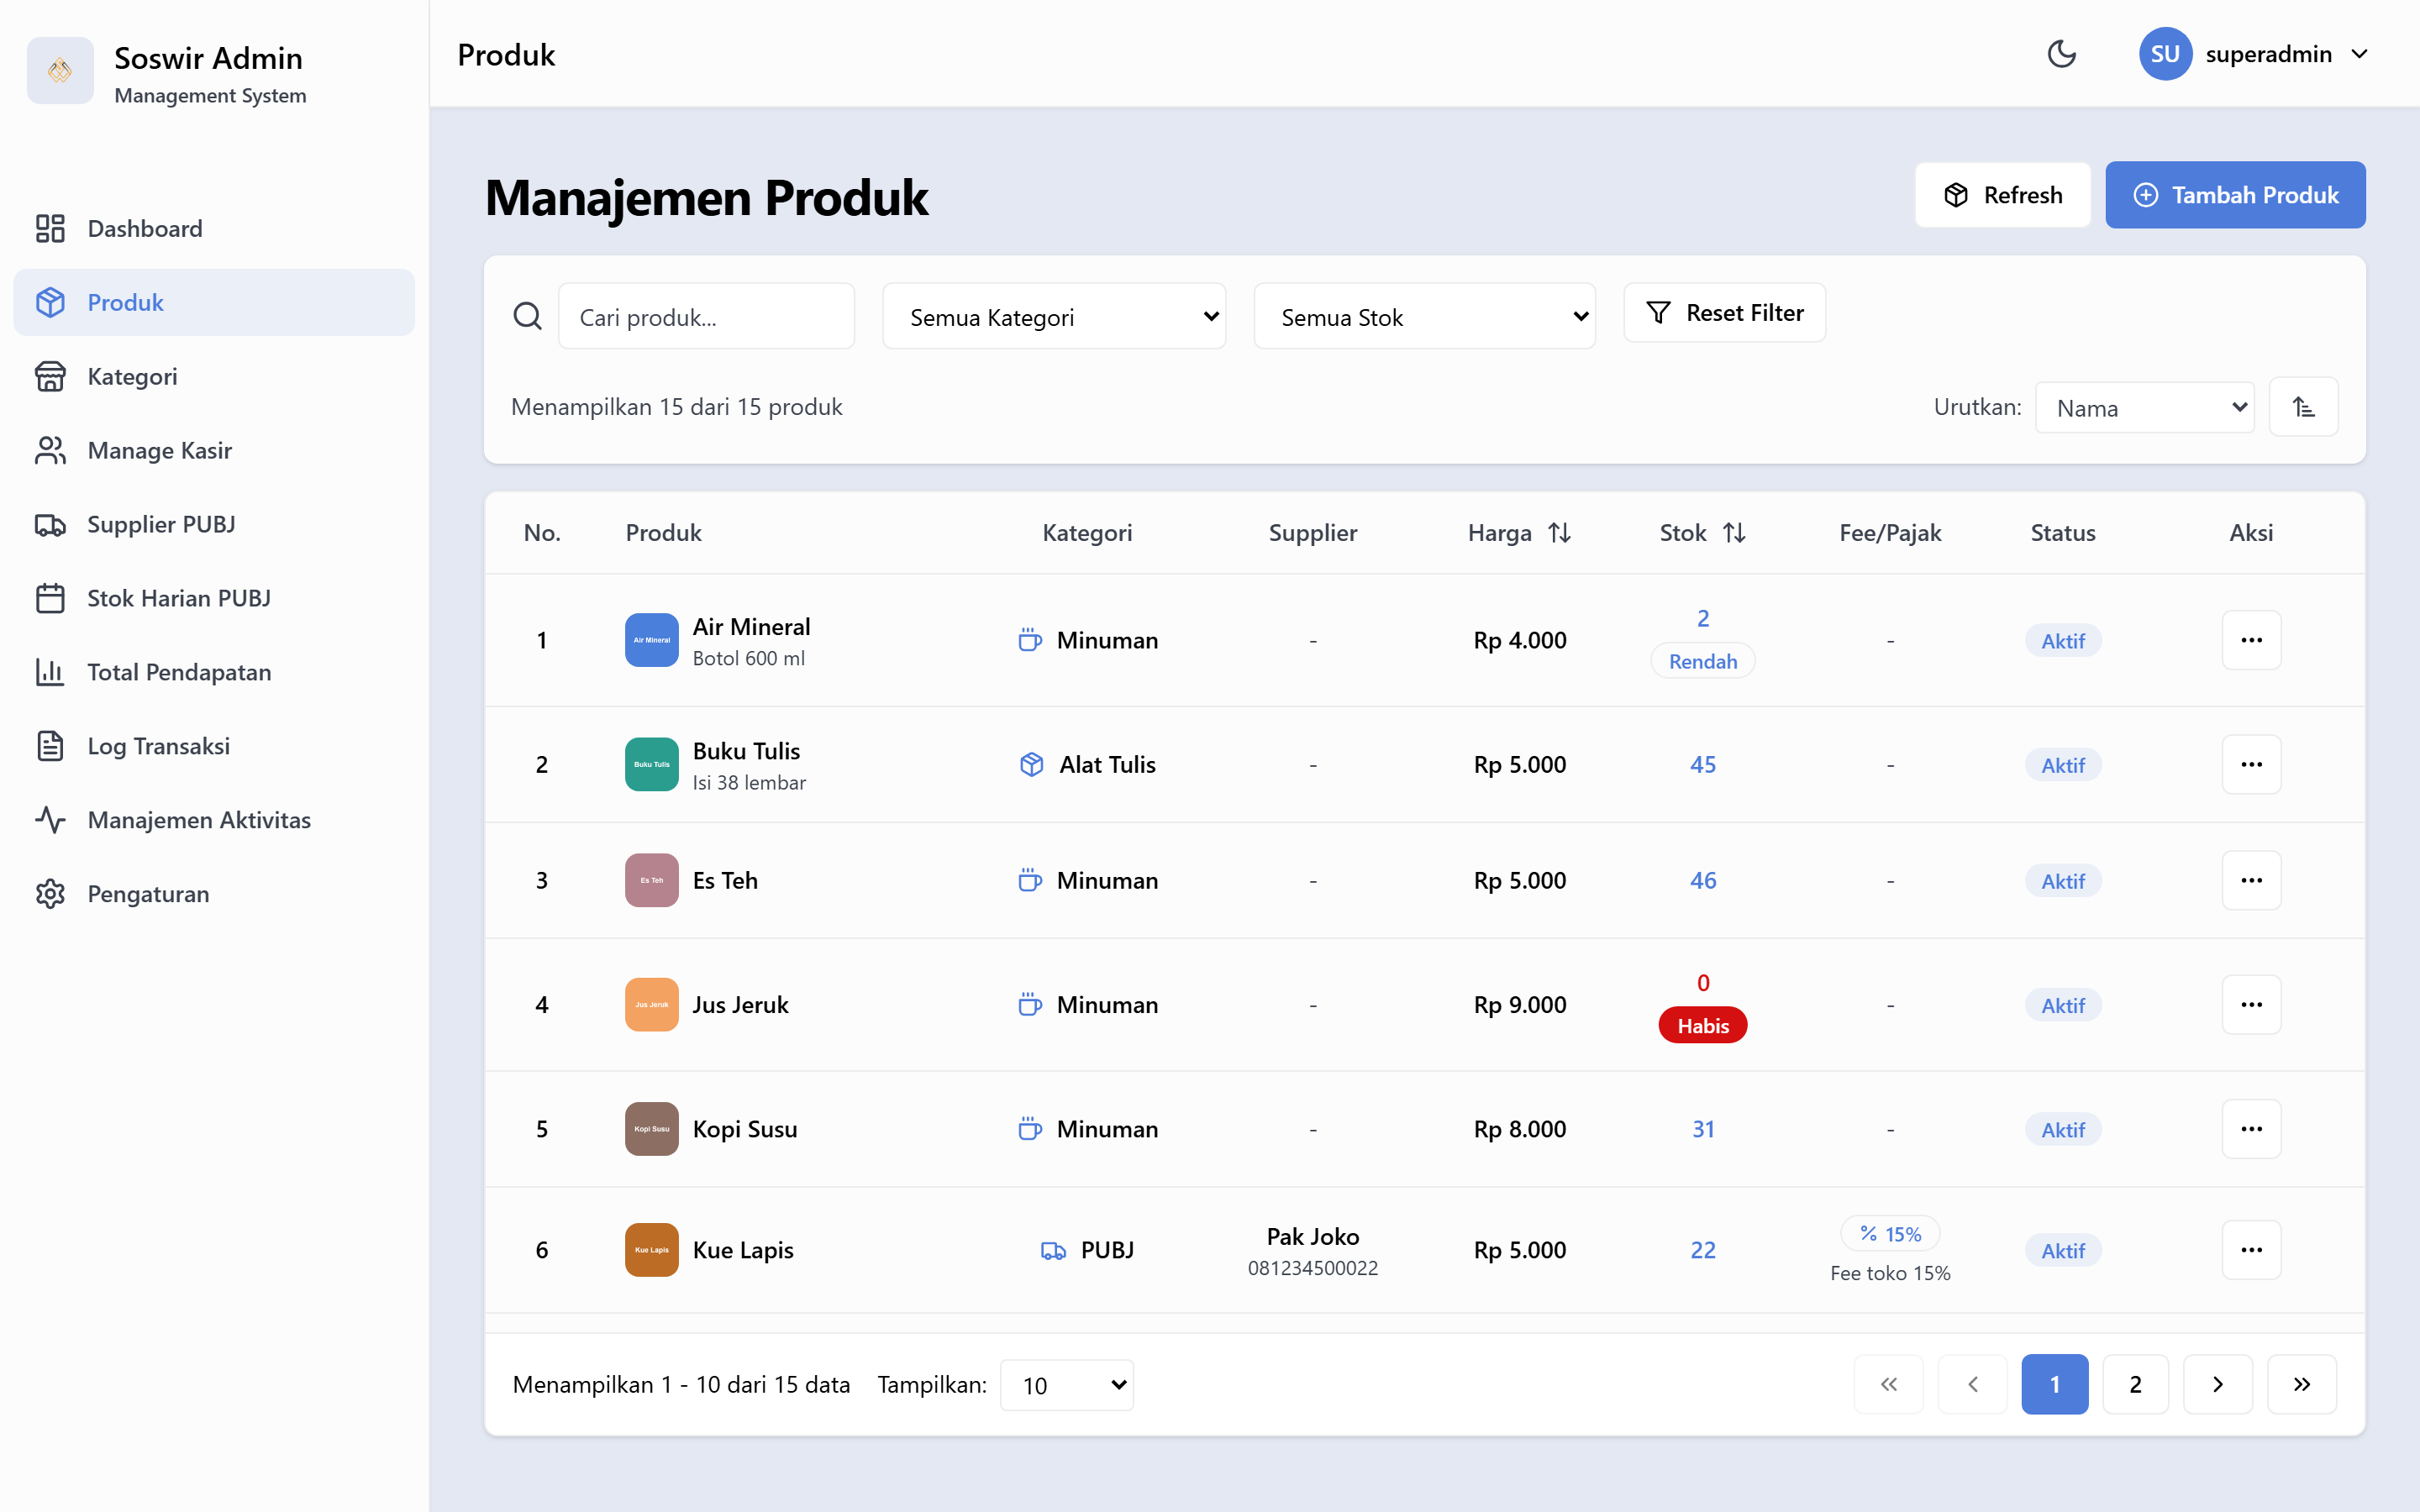
\includegraphics[width=0.99\linewidth,height=0.40\textheight,keepaspectratio,cfbox=garis 0.5pt 0pt]{img/15-produk-daftar.png}
\caption{Halaman \ui{Manajemen Produk}. Stok 0 ditandai \ui{Habis}, stok 10 ke bawah ditandai \ui{Rendah}.}
\end{figure}

Saring daftar dengan kotak \ui{Cari produk...}, pilihan \ui{Semua Kategori}, dan \ui{Semua Stok} (\ui{Stok Rendah (≤10)} atau \ui{Habis}).

\subsection{Menambah produk toko}

\begin{enumerate}
  \item Tekan \ui{Tambah Produk} di kanan atas.
  \item Isi \ui{Nama Produk} dan pilih \ui{Kategori}.
  \item Isi \ui{Harga (Rp)} dan \ui{Stok} awal. Stok harus bilangan bulat, boleh 0.
  \item Isi \ui{Deskripsi} bila perlu.
  \item Di bagian \ui{Gambar Produk}, tekan tombol pilih file pada \ui{Pilih Gambar} lalu pilih foto produk. Format yang diterima JPG, PNG, atau WEBP dengan ukuran paling besar 5 MB.
  \item Tekan \ui{Tambah Produk} di bagian bawah jendela.
\end{enumerate}

\begin{figure}[H]
\centering
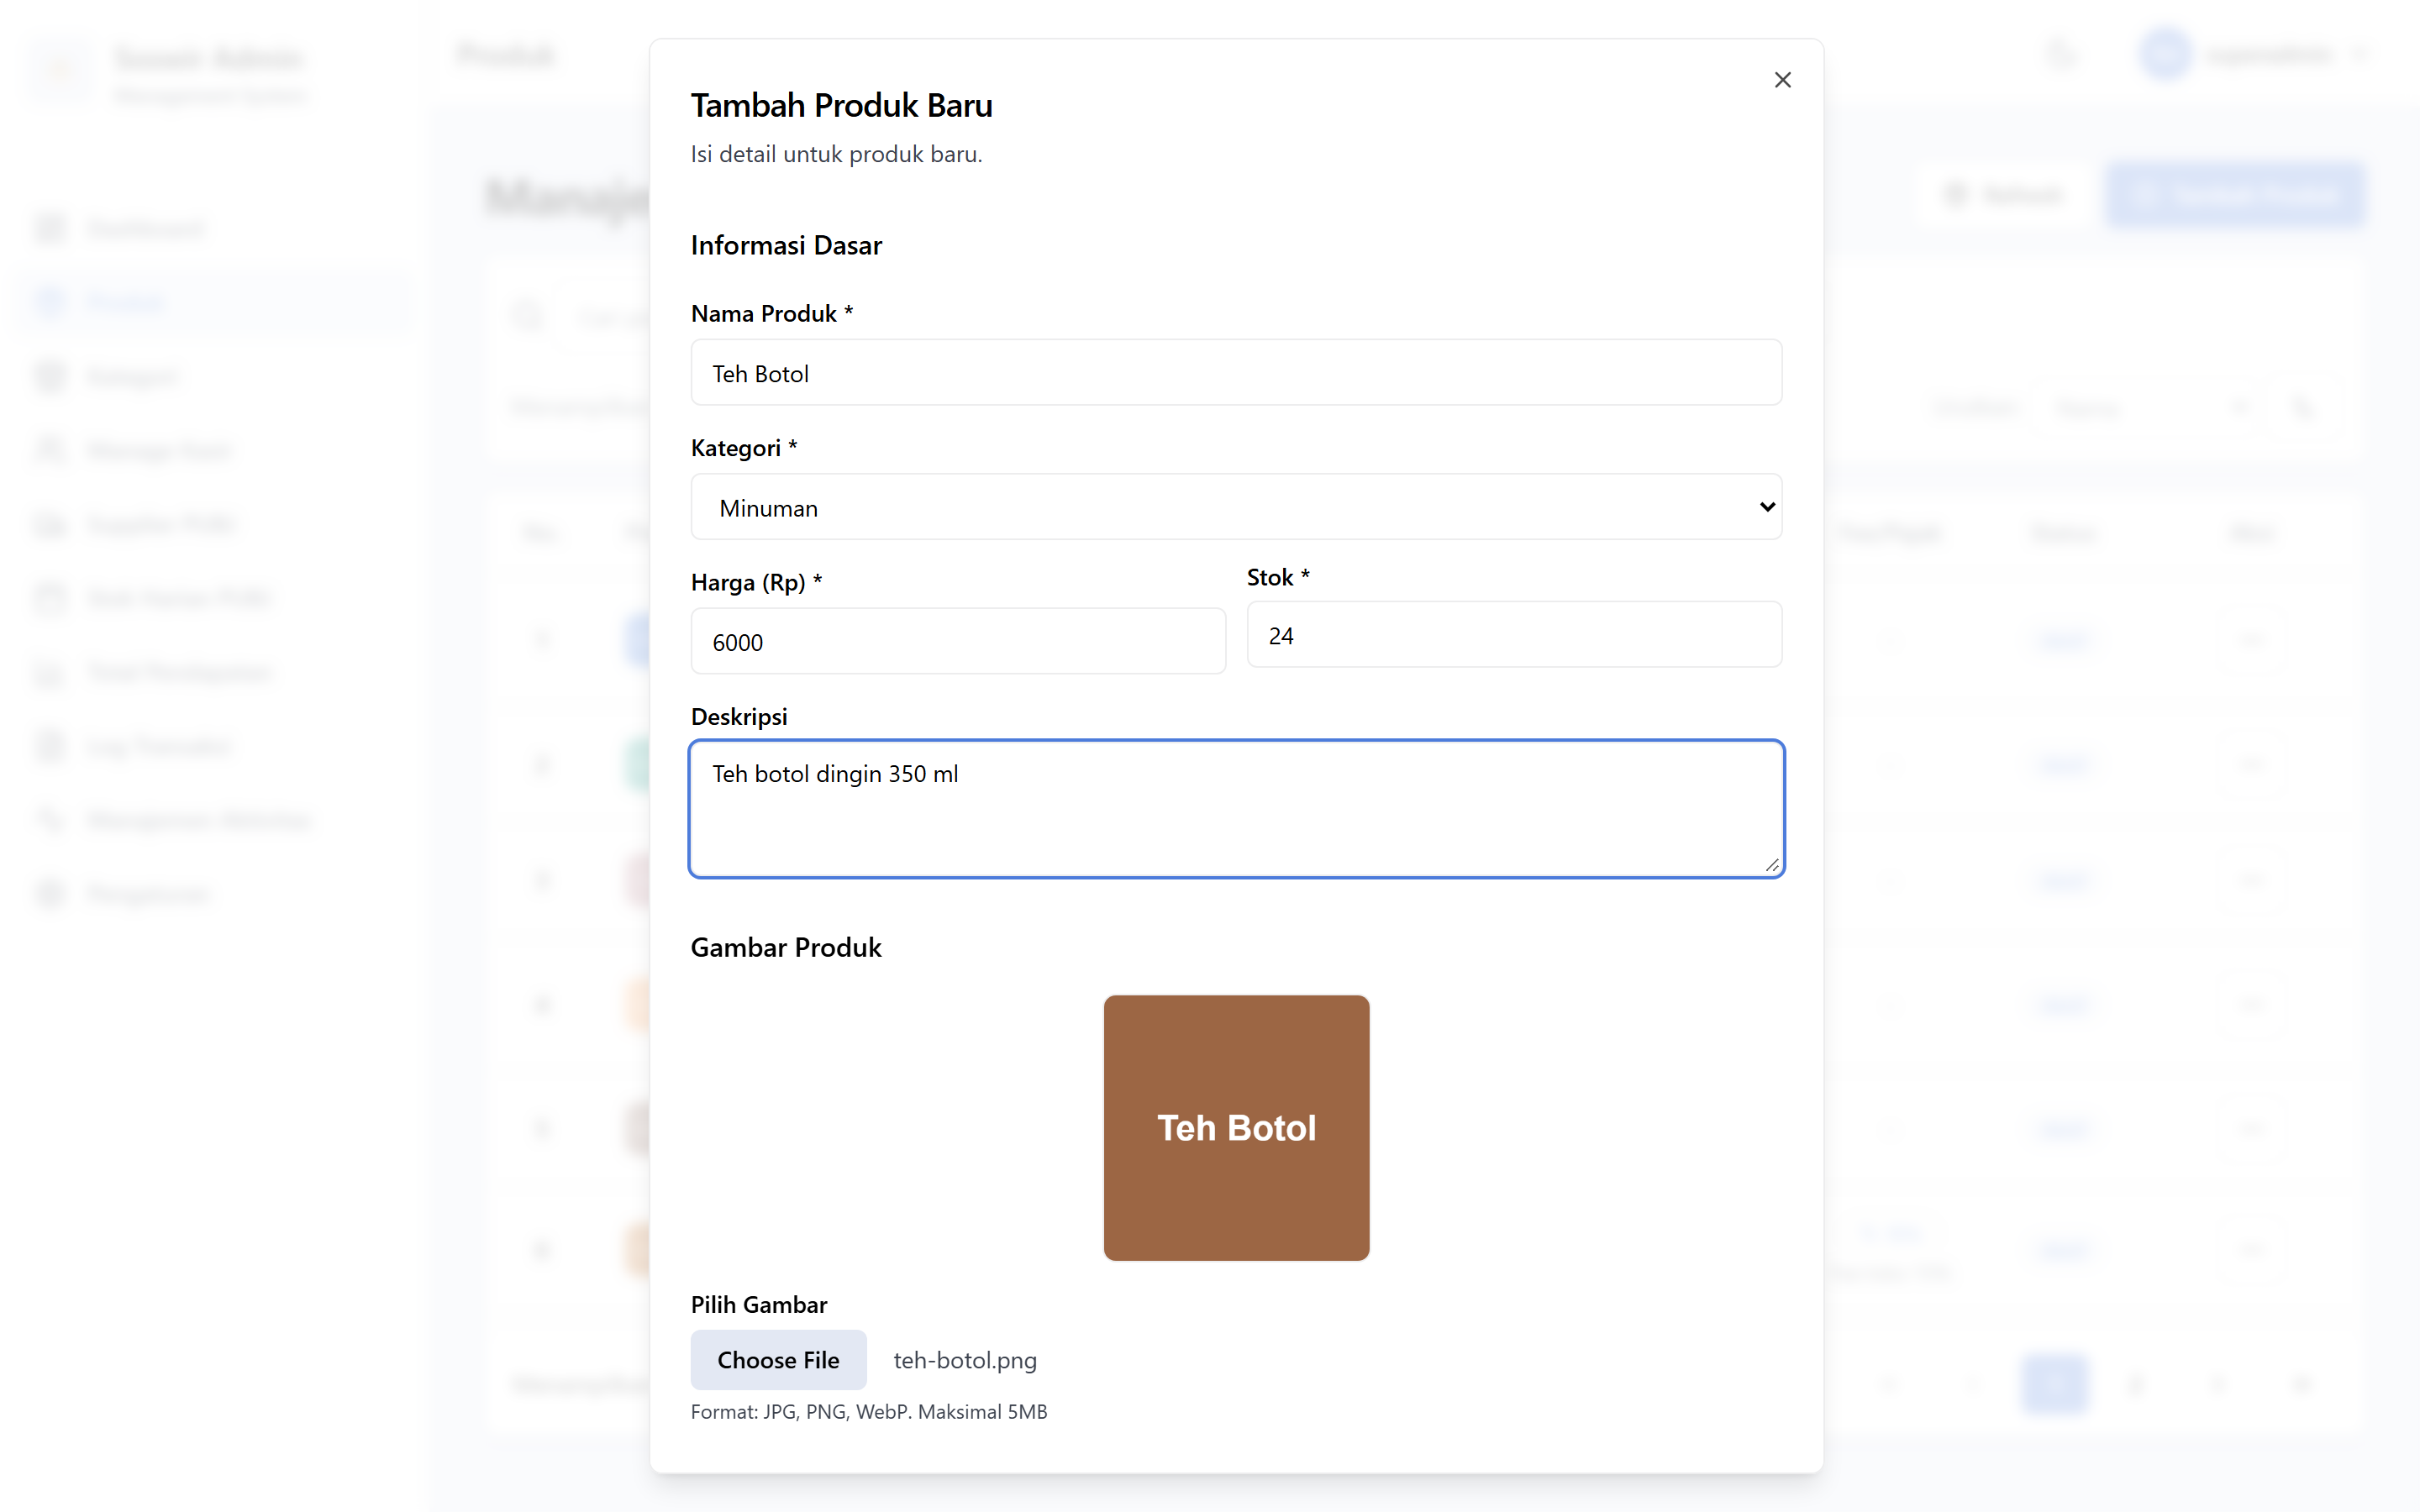
\includegraphics[width=0.99\linewidth,height=0.40\textheight,keepaspectratio,cfbox=garis 0.5pt 0pt]{img/16-produk-tambah.png}
\caption{Jendela \ui{Tambah Produk Baru} untuk produk toko.}
\end{figure}

\subsection{Menambah produk titipan (PUBJ)}

Produk titipan dibuat dengan cara yang sama, tetapi kategorinya kategori PUBJ.

\begin{enumerate}
  \item Tekan \ui{Tambah Produk}, isi nama dan harga jual, lalu pilih kategori PUBJ.
  \item Bagian \ui{Pengaturan PUBJ (Penitipan)} muncul. Pilih \ui{Supplier} pemilik barang.
  \item Isi \ui{Persentase Fee Toko (\%)}, yaitu bagian toko dari harga jual. \ui{Keterangan Fee} boleh diisi sebagai catatan.
  \item Periksa \ui{Simulasi Bagi Hasil:} untuk melihat bagian toko dan bagian supplier per unit.
  \item Tambahkan gambar, lalu tekan \ui{Tambah Produk}.
\end{enumerate}

\begin{figure}[H]
\centering
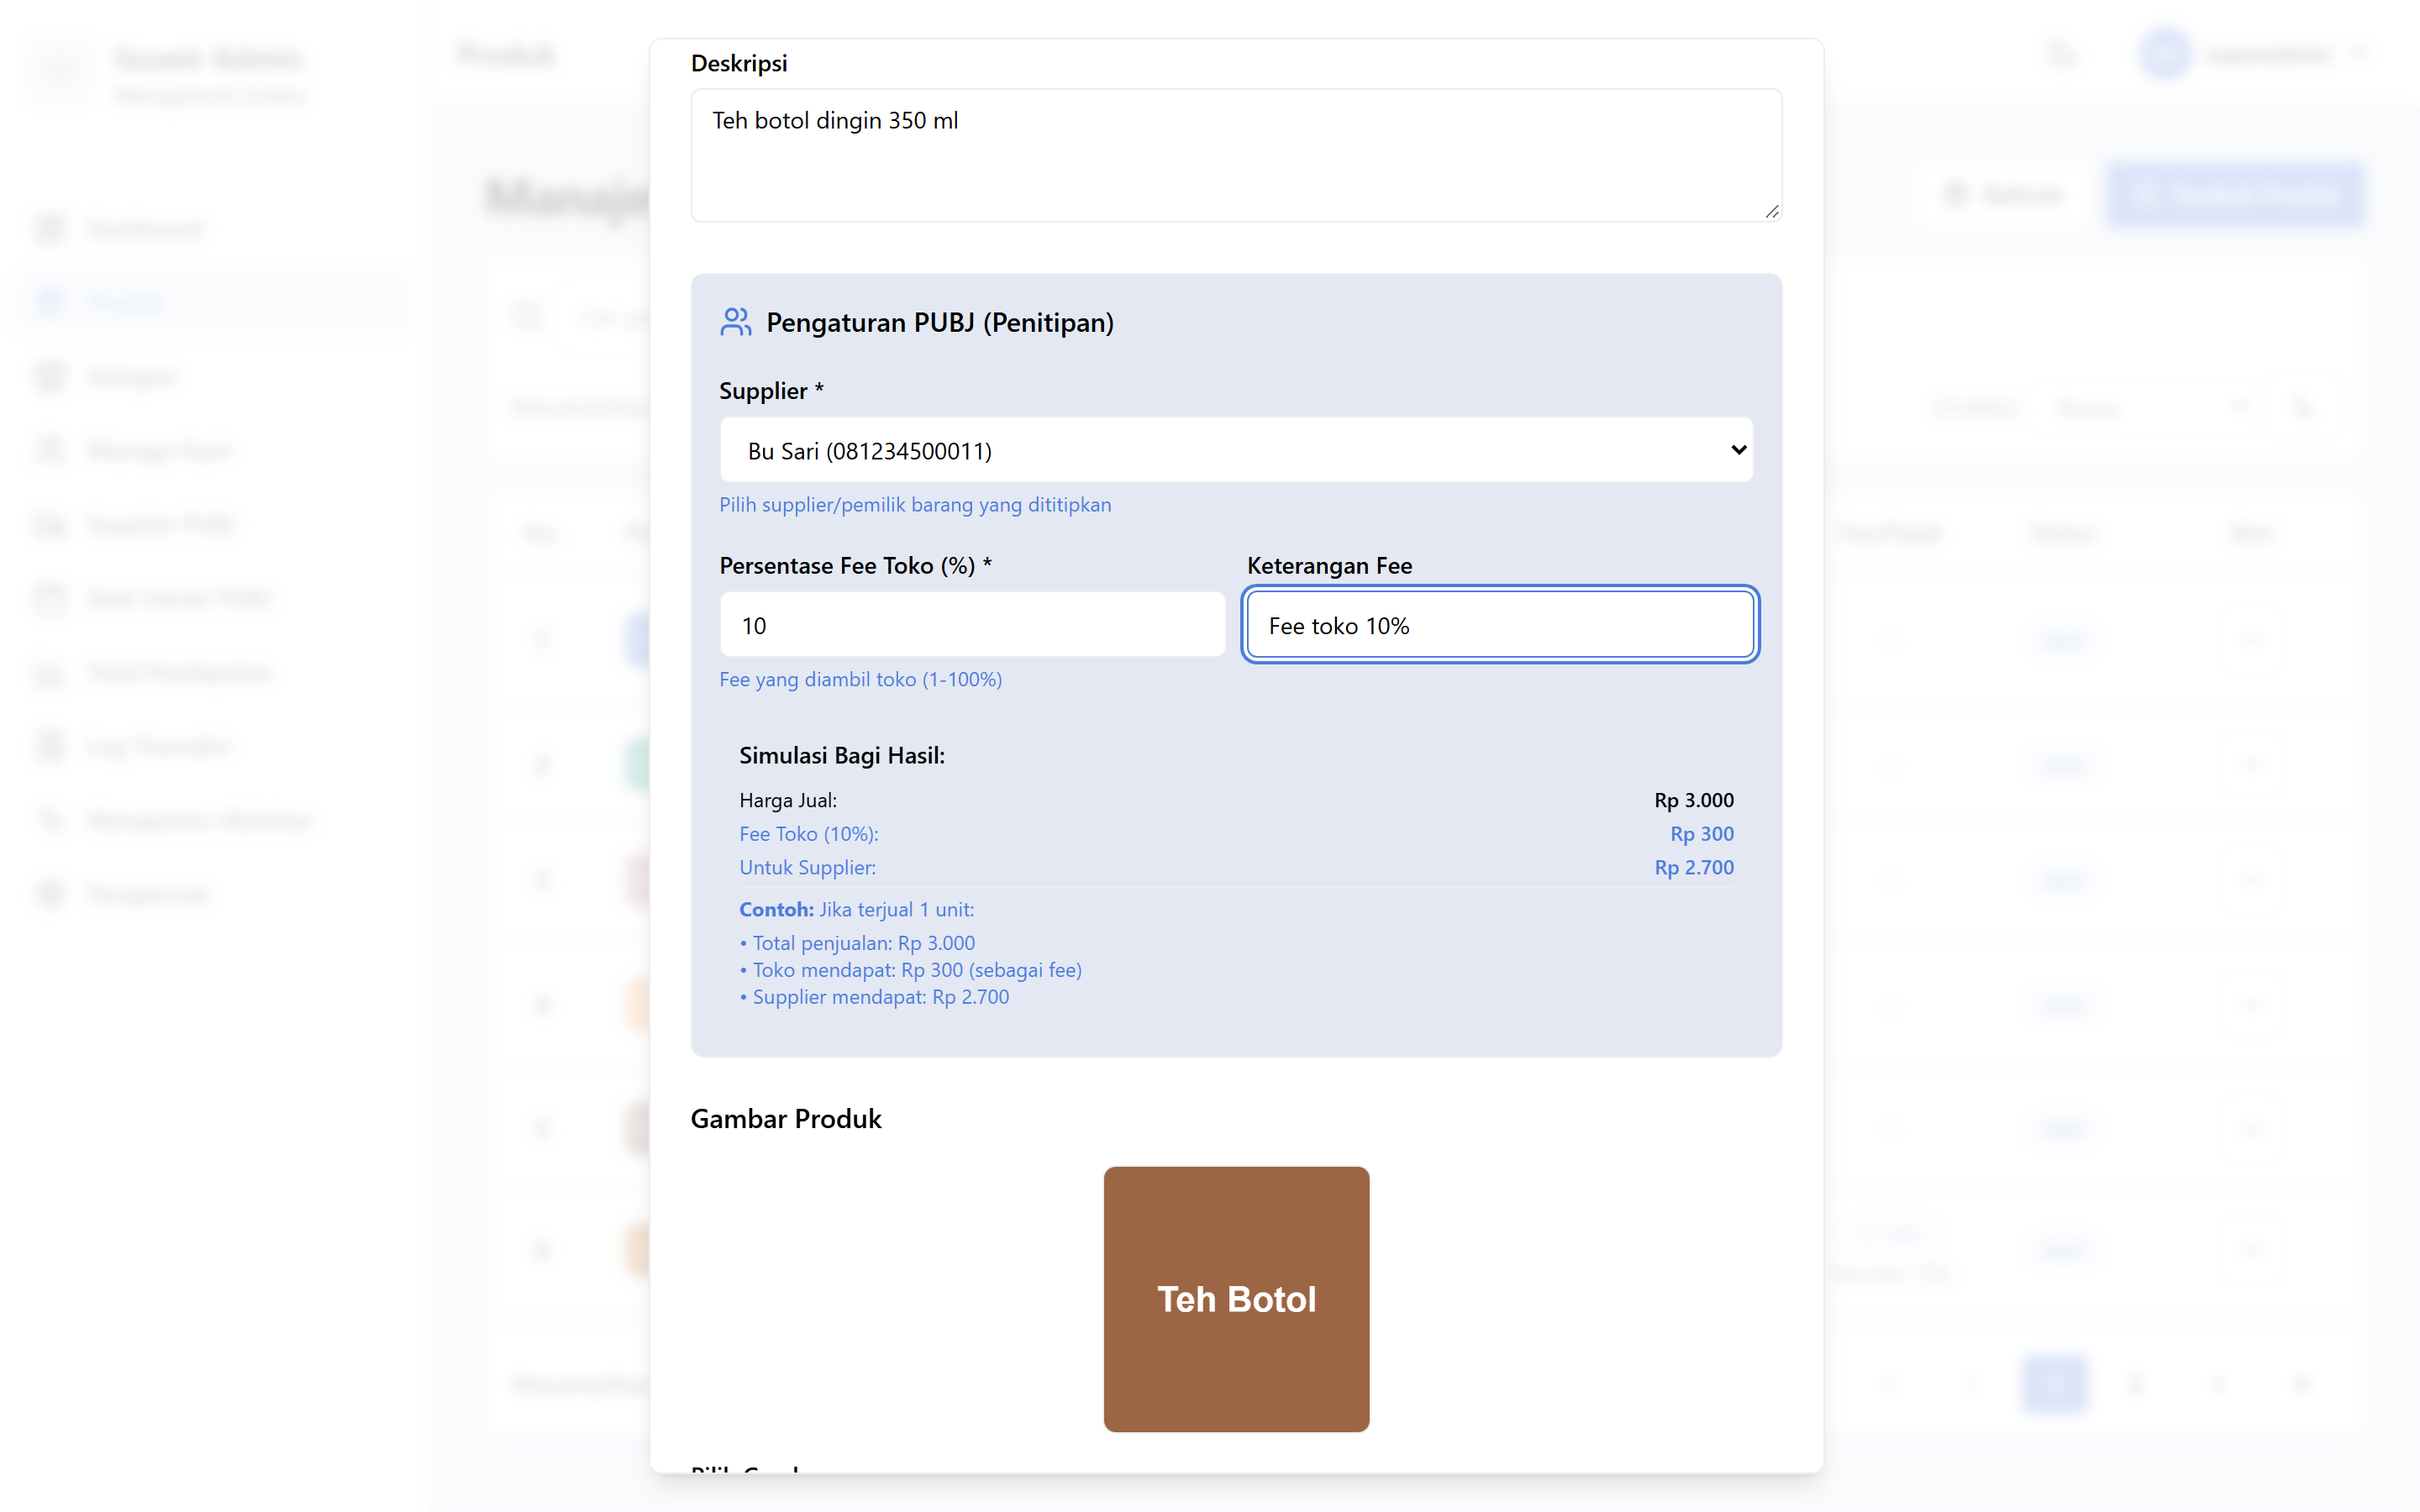
\includegraphics[width=0.99\linewidth,height=0.40\textheight,keepaspectratio,cfbox=garis 0.5pt 0pt]{img/17-produk-tambah-pubj.png}
\caption{Pengaturan PUBJ dengan simulasi bagi hasil fee toko 10\%.}
\end{figure}

\begin{catatan}
Kolom stok produk PUBJ tidak bisa diisi. Stoknya diambil otomatis dari \ui{Stok Harian PUBJ} hari ini.
\end{catatan}

\subsection{Mengubah produk}

\begin{enumerate}
  \item Tekan tombol tiga titik di kolom \ui{Aksi} pada baris produk.
  \item Pilih \ui{Edit}. Jendela \ui{Edit Produk} terbuka.
  \item Ubah nama, kategori, harga, deskripsi, atau gambar, lalu tekan \ui{Update Produk}.
\end{enumerate}

Stok tidak bisa diubah dari jendela \ui{Edit Produk}. Gunakan \ui{Tambah Stok} seperti di subbab berikut.

\begin{figure}[H]
\centering
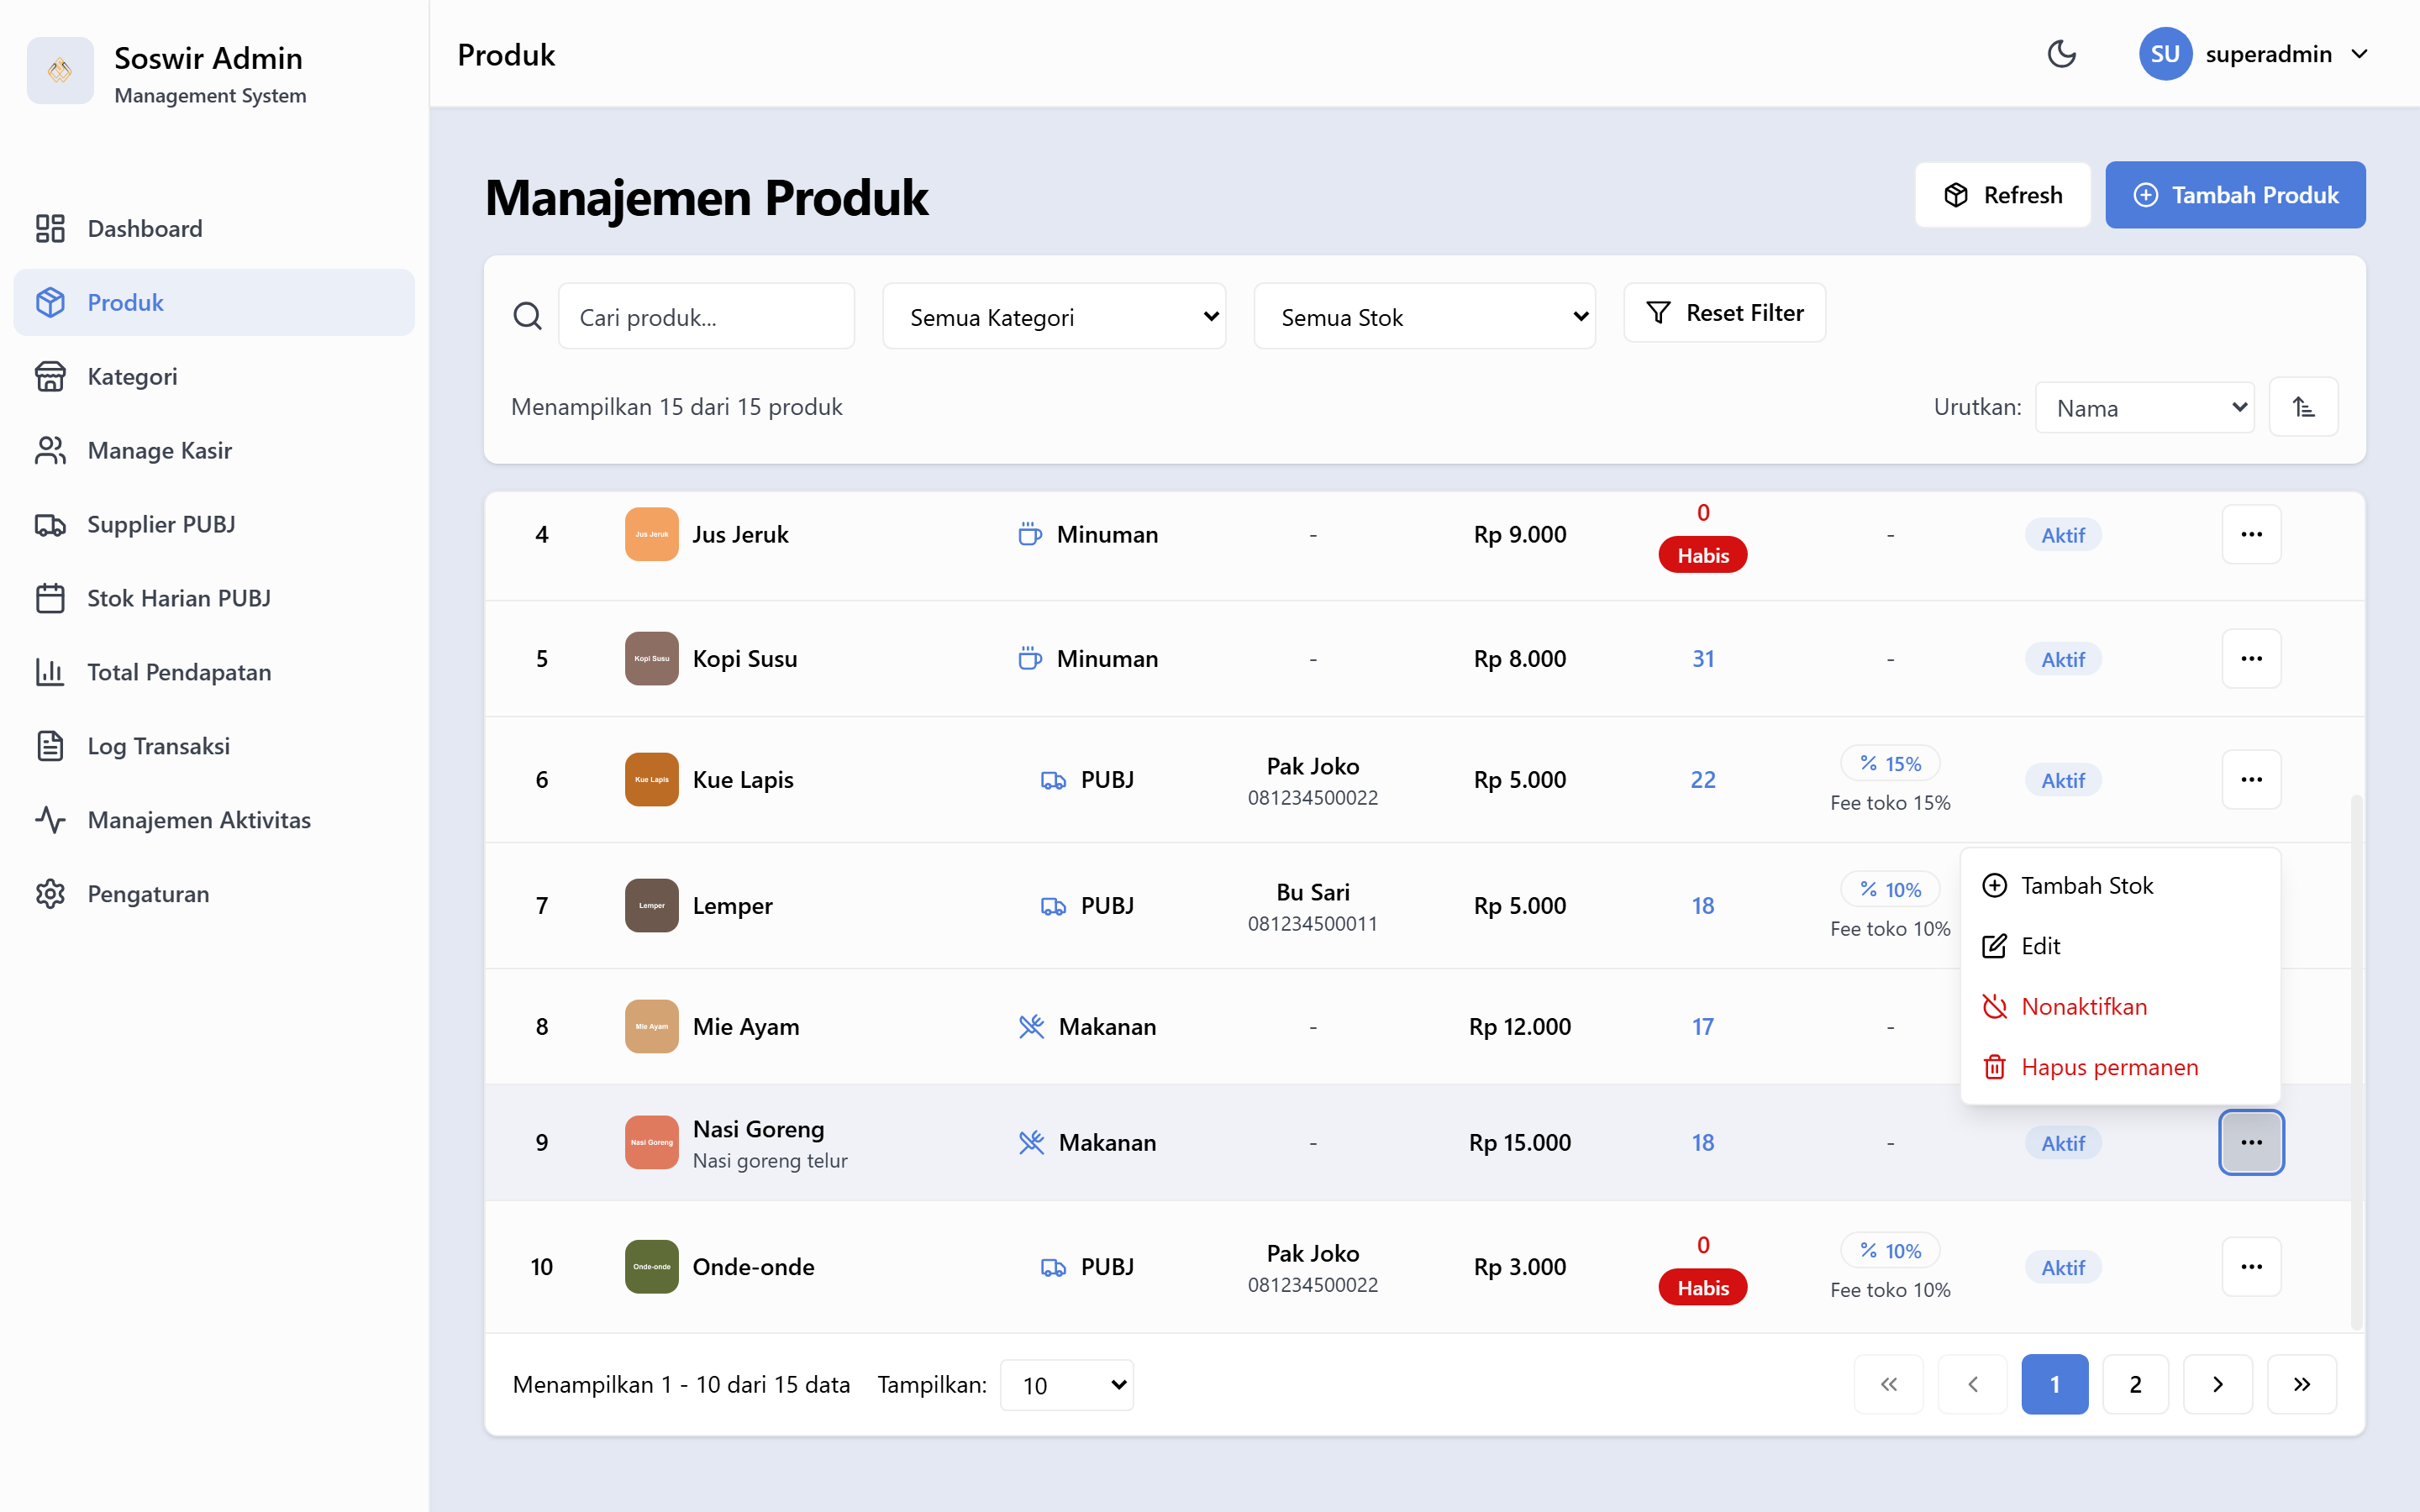
\includegraphics[width=0.99\linewidth,height=0.40\textheight,keepaspectratio,cfbox=garis 0.5pt 0pt]{img/18-produk-menu-aksi.png}
\caption{Menu aksi produk: \ui{Tambah Stok}, \ui{Edit}, \ui{Nonaktifkan}, dan \ui{Hapus permanen}.}
\end{figure}

\subsection{Menambah stok produk toko}

Pakai cara ini saat barang toko datang.

\begin{enumerate}
  \item Buka menu aksi produk, pilih \ui{Tambah Stok}.
  \item Isi \ui{Jumlah stok tambahan} dengan bilangan bulat lebih dari 0. Jendela menampilkan \ui{Stok saat ini} dan \ui{Stok setelah ditambah}.
  \item Tekan \ui{Tambah Stok}.
\end{enumerate}

\begin{figure}[H]
\centering
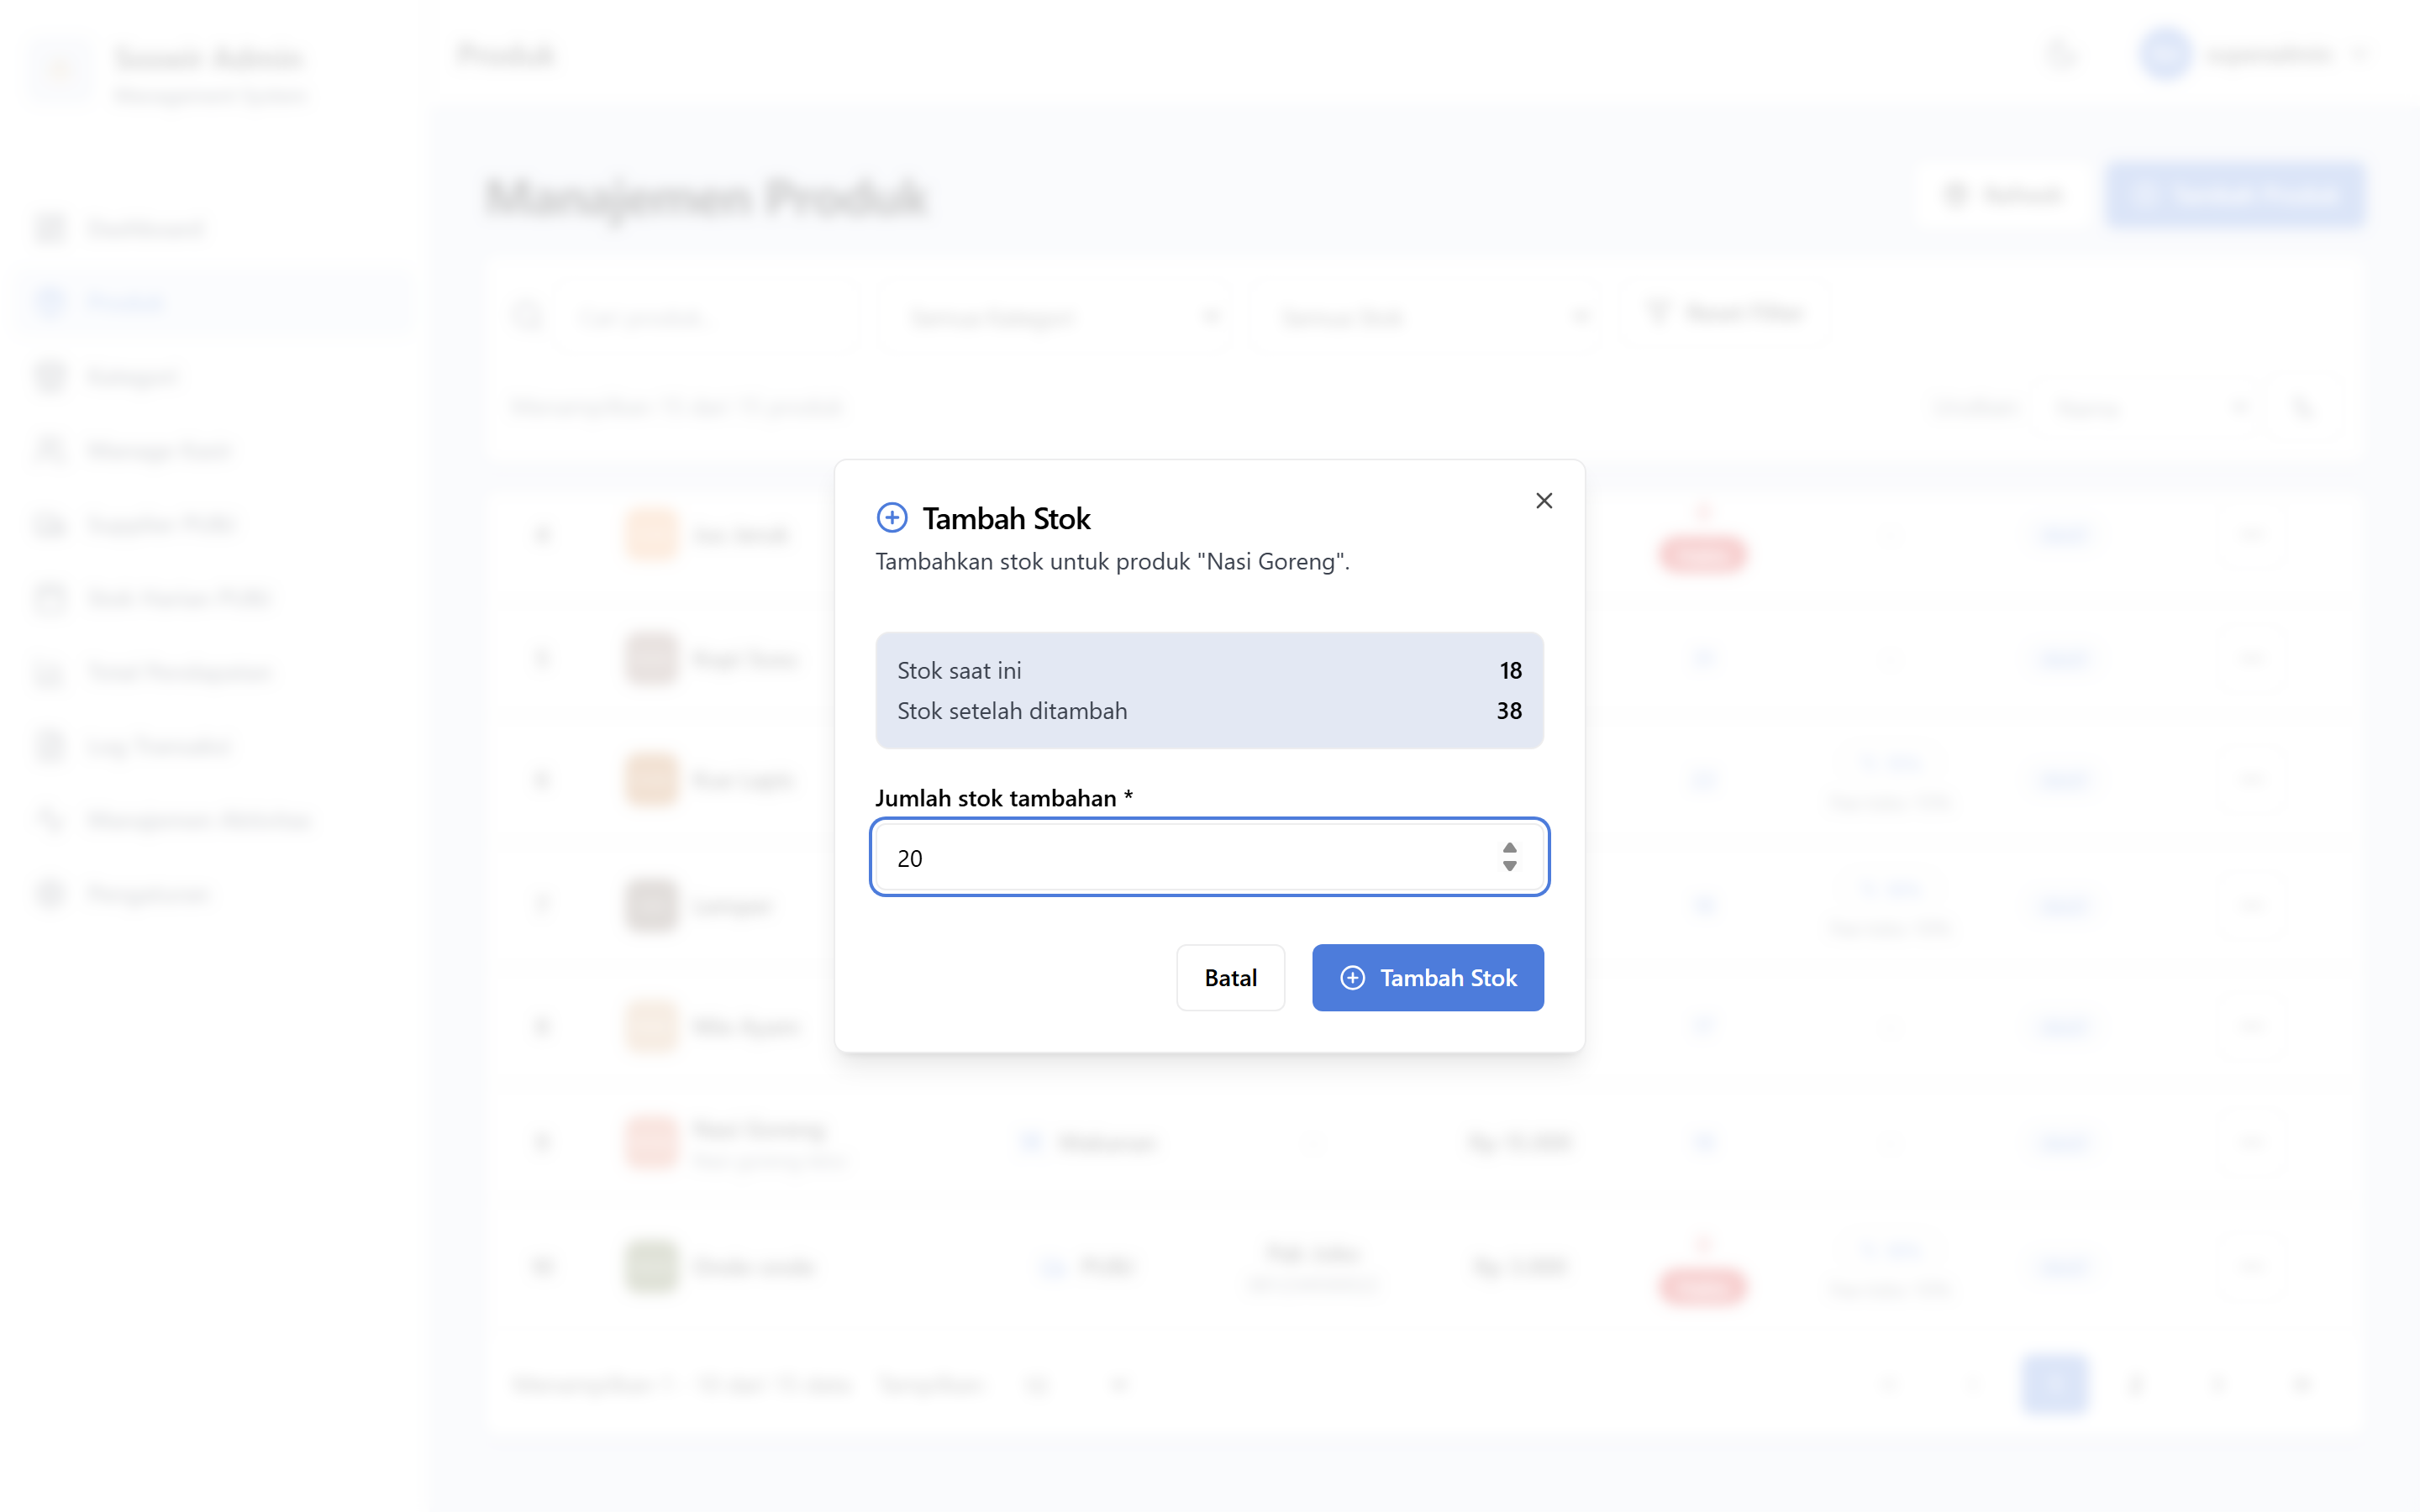
\includegraphics[width=0.99\linewidth,height=0.40\textheight,keepaspectratio,cfbox=garis 0.5pt 0pt]{img/19-produk-tambah-stok.png}
\caption{Jendela \ui{Tambah Stok}.}
\end{figure}

Pilihan \ui{Tambah Stok} tidak ada untuk produk PUBJ. Stok titipan ditambah lewat \ui{Stok Harian PUBJ}.

\subsection{Menonaktifkan dan mengaktifkan produk}

Produk yang tidak dijual sementara cukup dinonaktifkan. Produk nonaktif tidak muncul di kasir, tetapi datanya dan riwayat penjualannya tetap ada.

\begin{enumerate}
  \item Buka menu aksi produk, pilih \ui{Nonaktifkan}.
  \item Periksa nama produk di jendela \ui{Konfirmasi Perubahan Status}, lalu tekan \ui{Nonaktifkan}.
  \item Untuk menjual lagi, buka menu aksi yang sama dan pilih \ui{Aktifkan}.
\end{enumerate}

\begin{figure}[H]
\centering
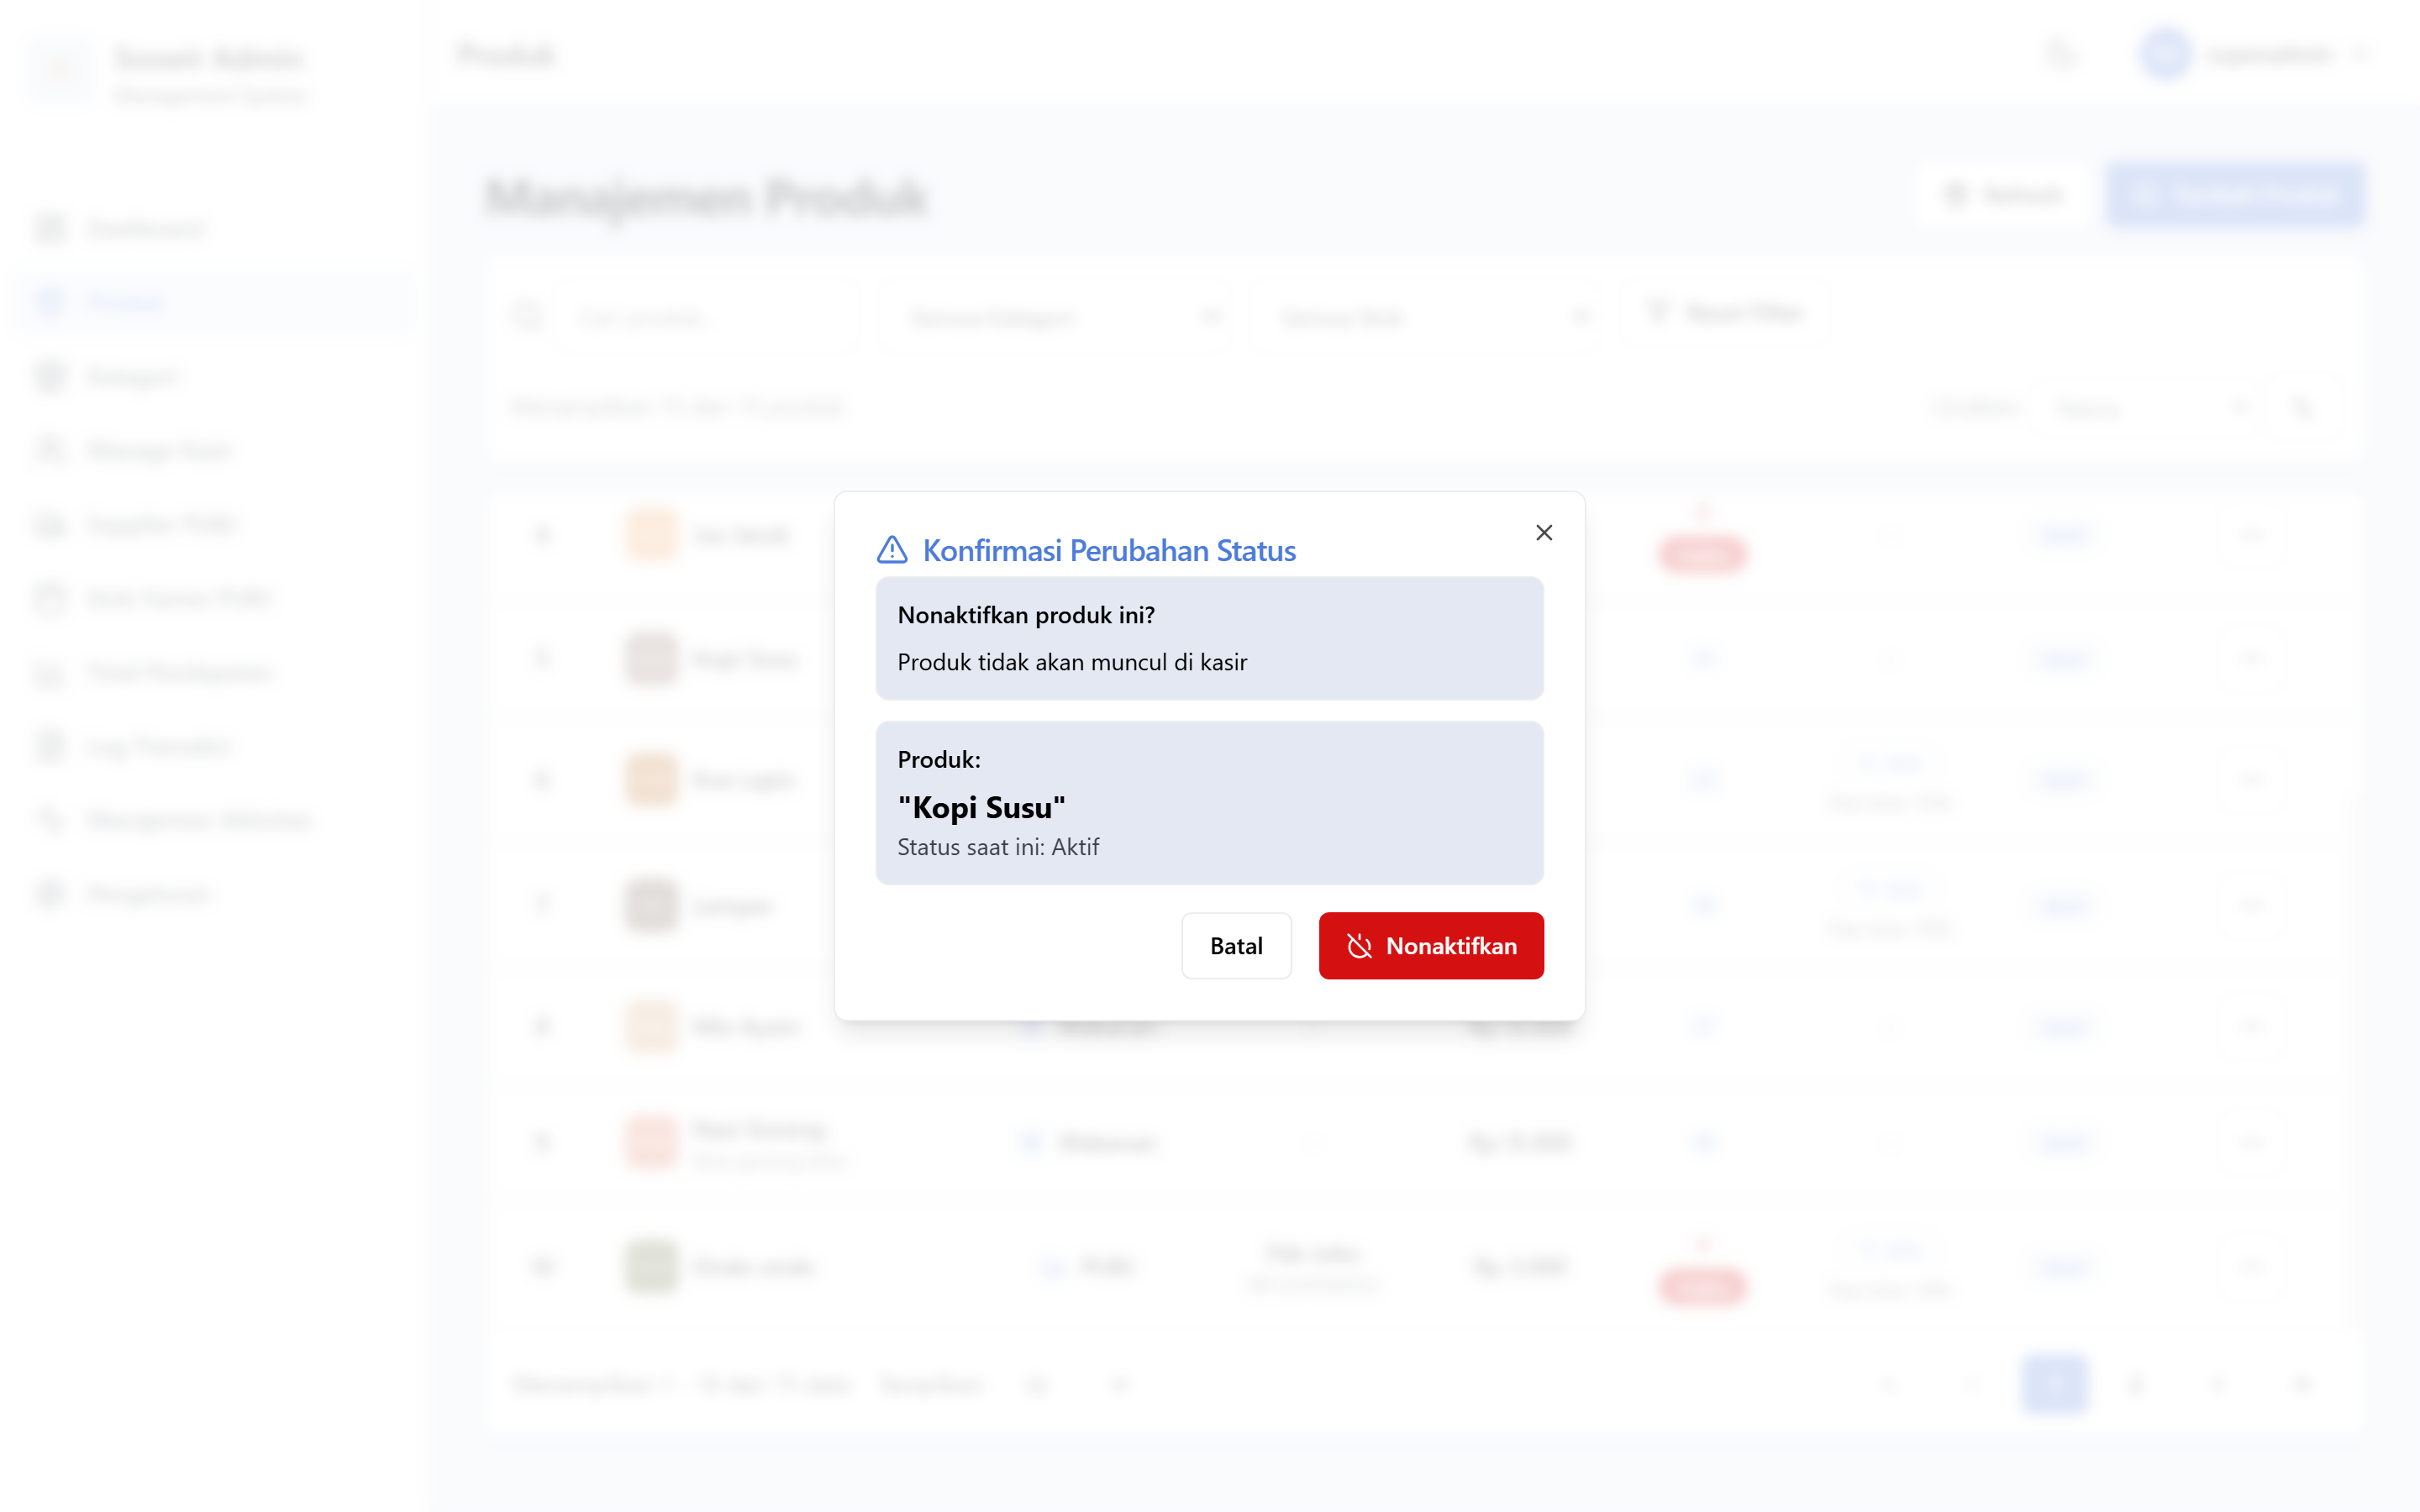
\includegraphics[width=0.99\linewidth,height=0.40\textheight,keepaspectratio,cfbox=garis 0.5pt 0pt]{img/20-produk-nonaktifkan.png}
\caption{Konfirmasi menonaktifkan produk.}
\end{figure}

\subsection{Menghapus produk secara permanen}

Hapus permanen menghilangkan produk dan gambarnya dari sistem, dan tidak bisa dibatalkan.

\begin{enumerate}
  \item Buka menu aksi produk, pilih \ui{Hapus permanen}.
  \item Baca peringatan di jendela \ui{Hapus Produk Secara Permanen}.
  \item Ketik password superadmin Anda di kolom \ui{Masukkan Password Anda untuk Konfirmasi}.
  \item Tekan \ui{Hapus Permanen}.
\end{enumerate}

\begin{figure}[H]
\centering
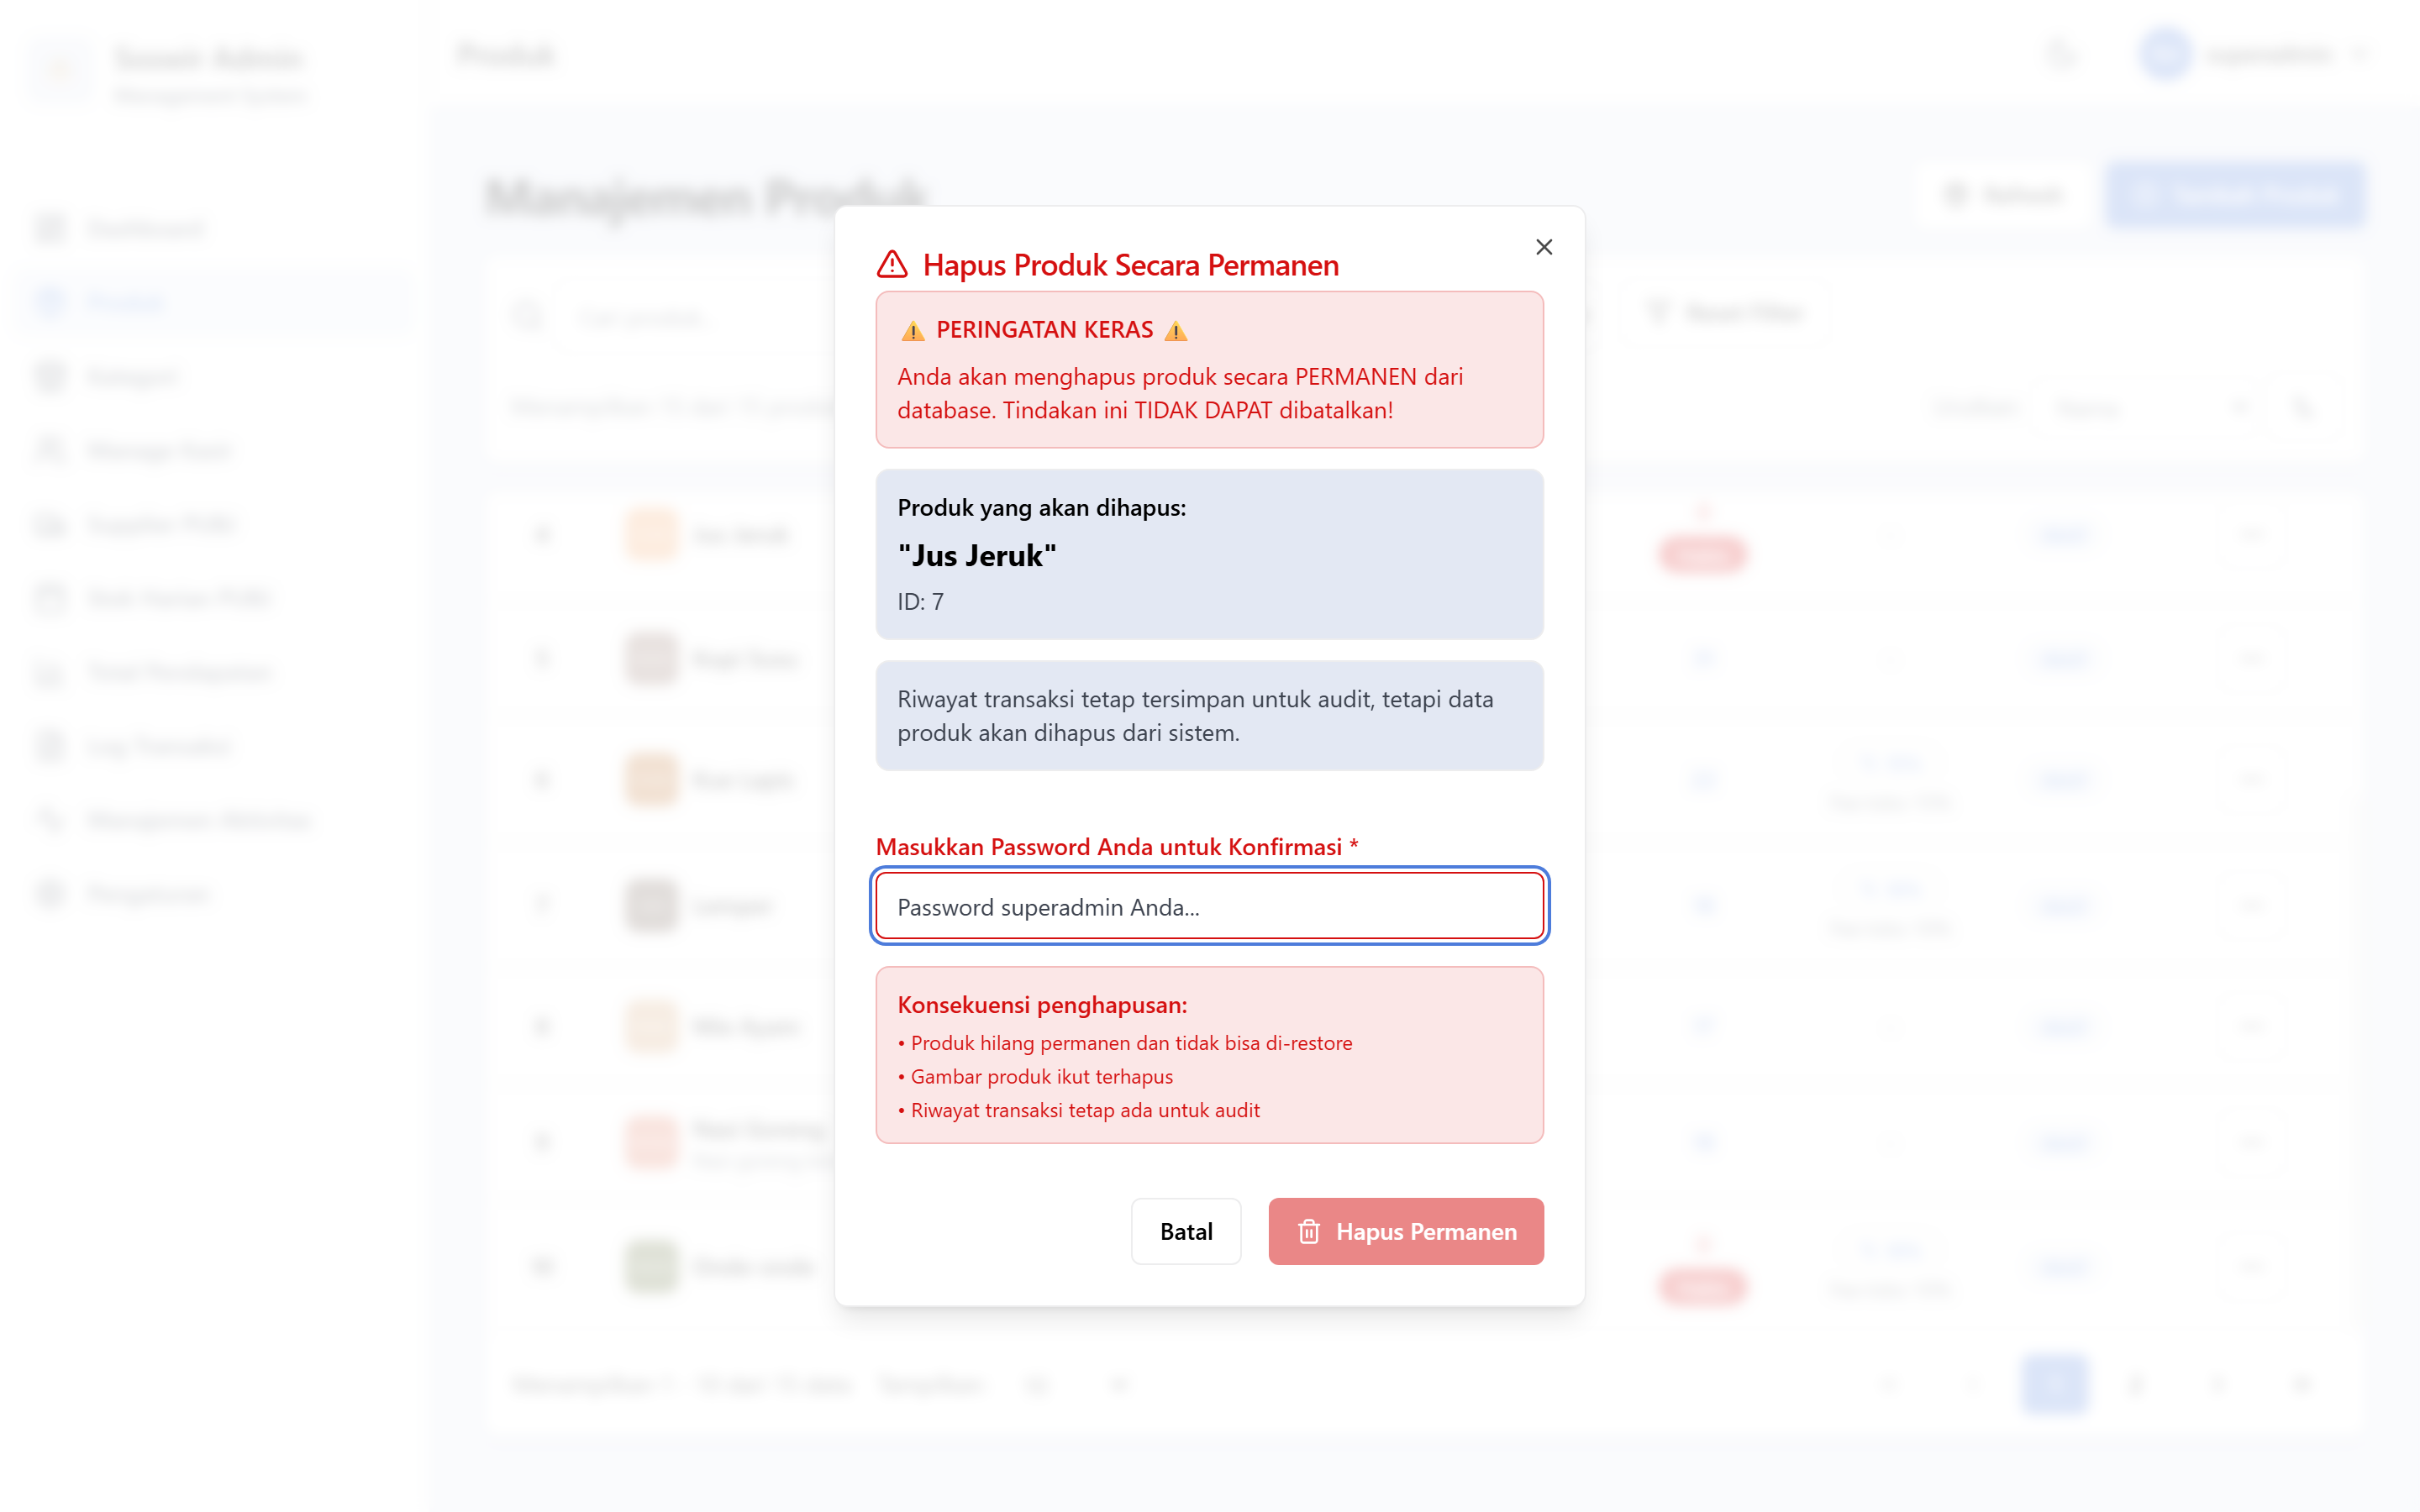
\includegraphics[width=0.99\linewidth,height=0.40\textheight,keepaspectratio,cfbox=garis 0.5pt 0pt]{img/21-produk-hapus-permanen.png}
\caption{Hapus permanen meminta password superadmin.}
\end{figure}

\begin{catatan}
Produk yang sudah pernah terjual atau sudah punya stok harian PUBJ tidak bisa dihapus permanen. Aplikasi menolak dan menyebut jumlah riwayat yang masih terkait. Untuk produk seperti itu, pakai \ui{Nonaktifkan}.
\end{catatan}

% ---------------------------------------------------------------
\section{Kategori}

Menu \ui{Kategori} membuka halaman \ui{Manajemen Kategori}. Setiap produk wajib masuk ke satu kategori.

Ada dua tipe kategori:

\begin{itemize}
  \item \ui{Toko}: barang milik toko sendiri. Seluruh hasil penjualan menjadi keuntungan toko, dan stoknya dikelola lewat \ui{Tambah Stok}.
  \item \ui{PUBJ}: barang titipan supplier. Toko hanya mengambil fee sesuai persentase tiap produk, sisanya menjadi hak supplier. Stoknya dicatat setiap hari lewat \ui{Stok Harian PUBJ}.
\end{itemize}

\begin{figure}[H]
\centering
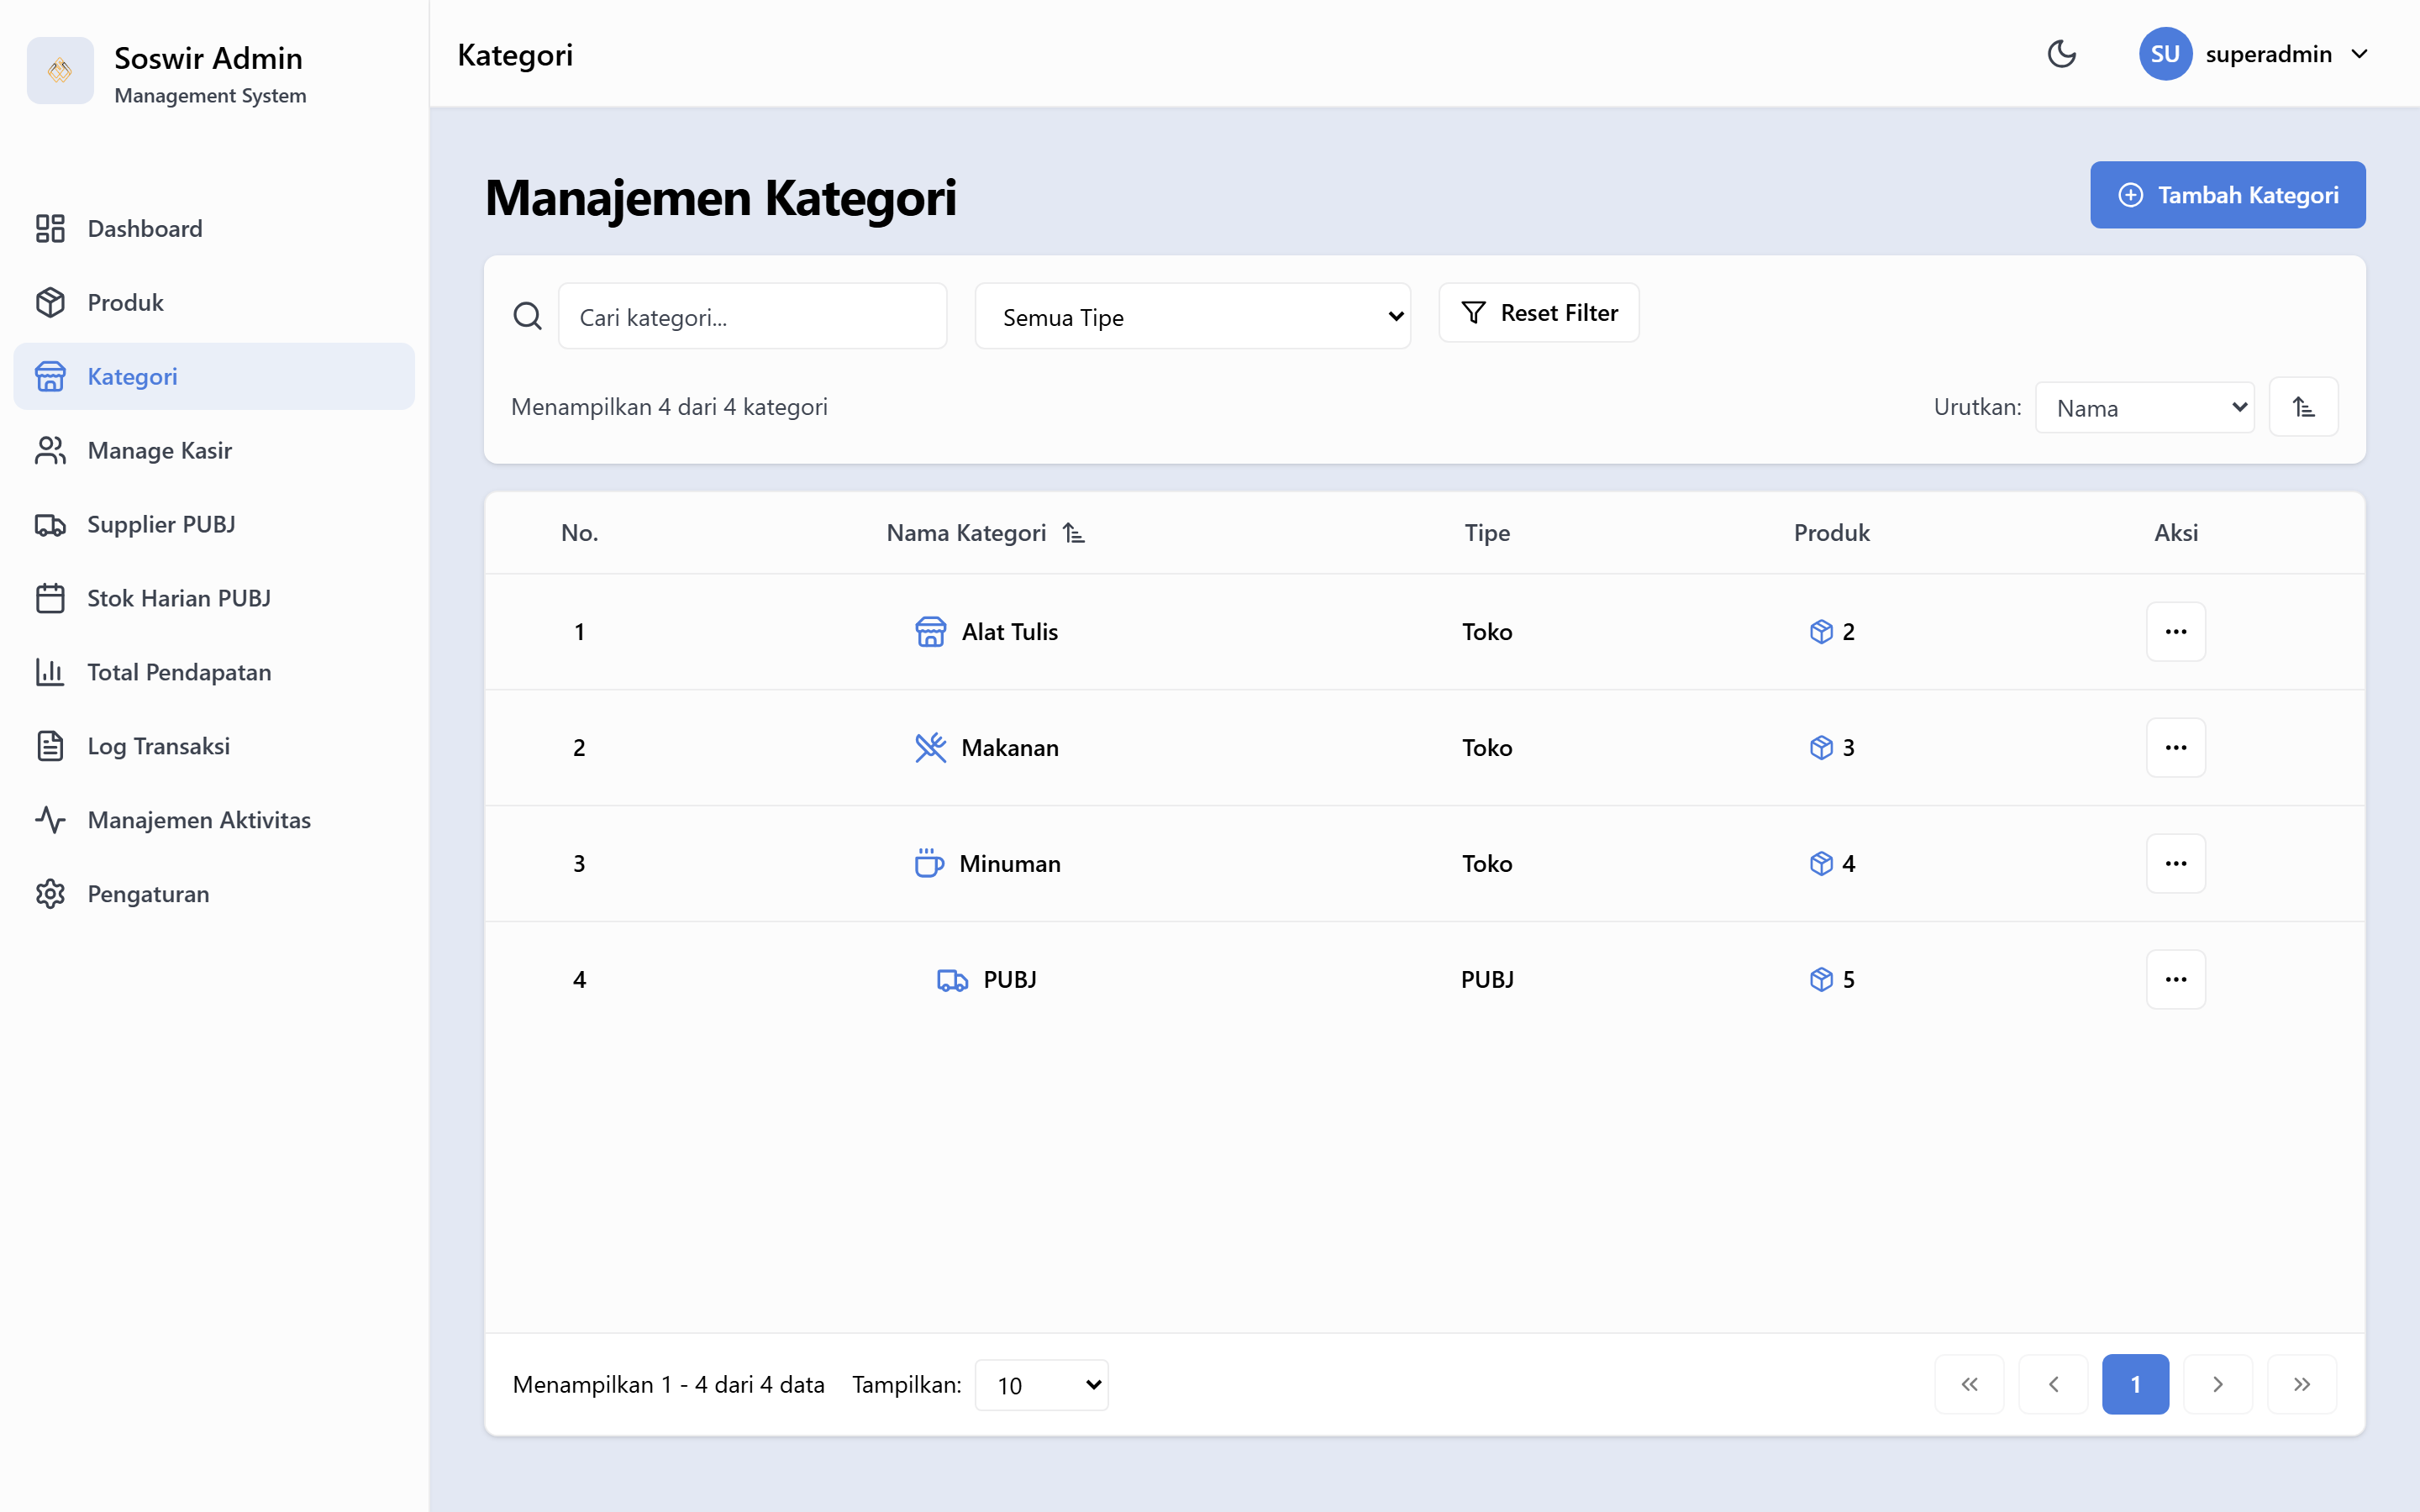
\includegraphics[width=0.99\linewidth,height=0.40\textheight,keepaspectratio,cfbox=garis 0.5pt 0pt]{img/22-kategori-daftar.png}
\caption{Daftar kategori beserta tipe dan jumlah produknya.}
\end{figure}

\subsection{Menambah dan mengubah kategori}

\begin{enumerate}
  \item Tekan \ui{Tambah Kategori}. Untuk mengubah, buka menu aksi kategori lalu pilih \ui{Edit}.
  \item Isi \ui{Nama} dan \ui{Deskripsi}.
  \item Atur sakelar \ui{Jenis Kategori}. Posisi mati berarti \ui{Produk Toko}; posisi menyala berarti \ui{Penitipan/Reseller (PUBJ)}.
  \item Tekan \ui{Simpan}.
\end{enumerate}

\begin{figure}[H]
\centering
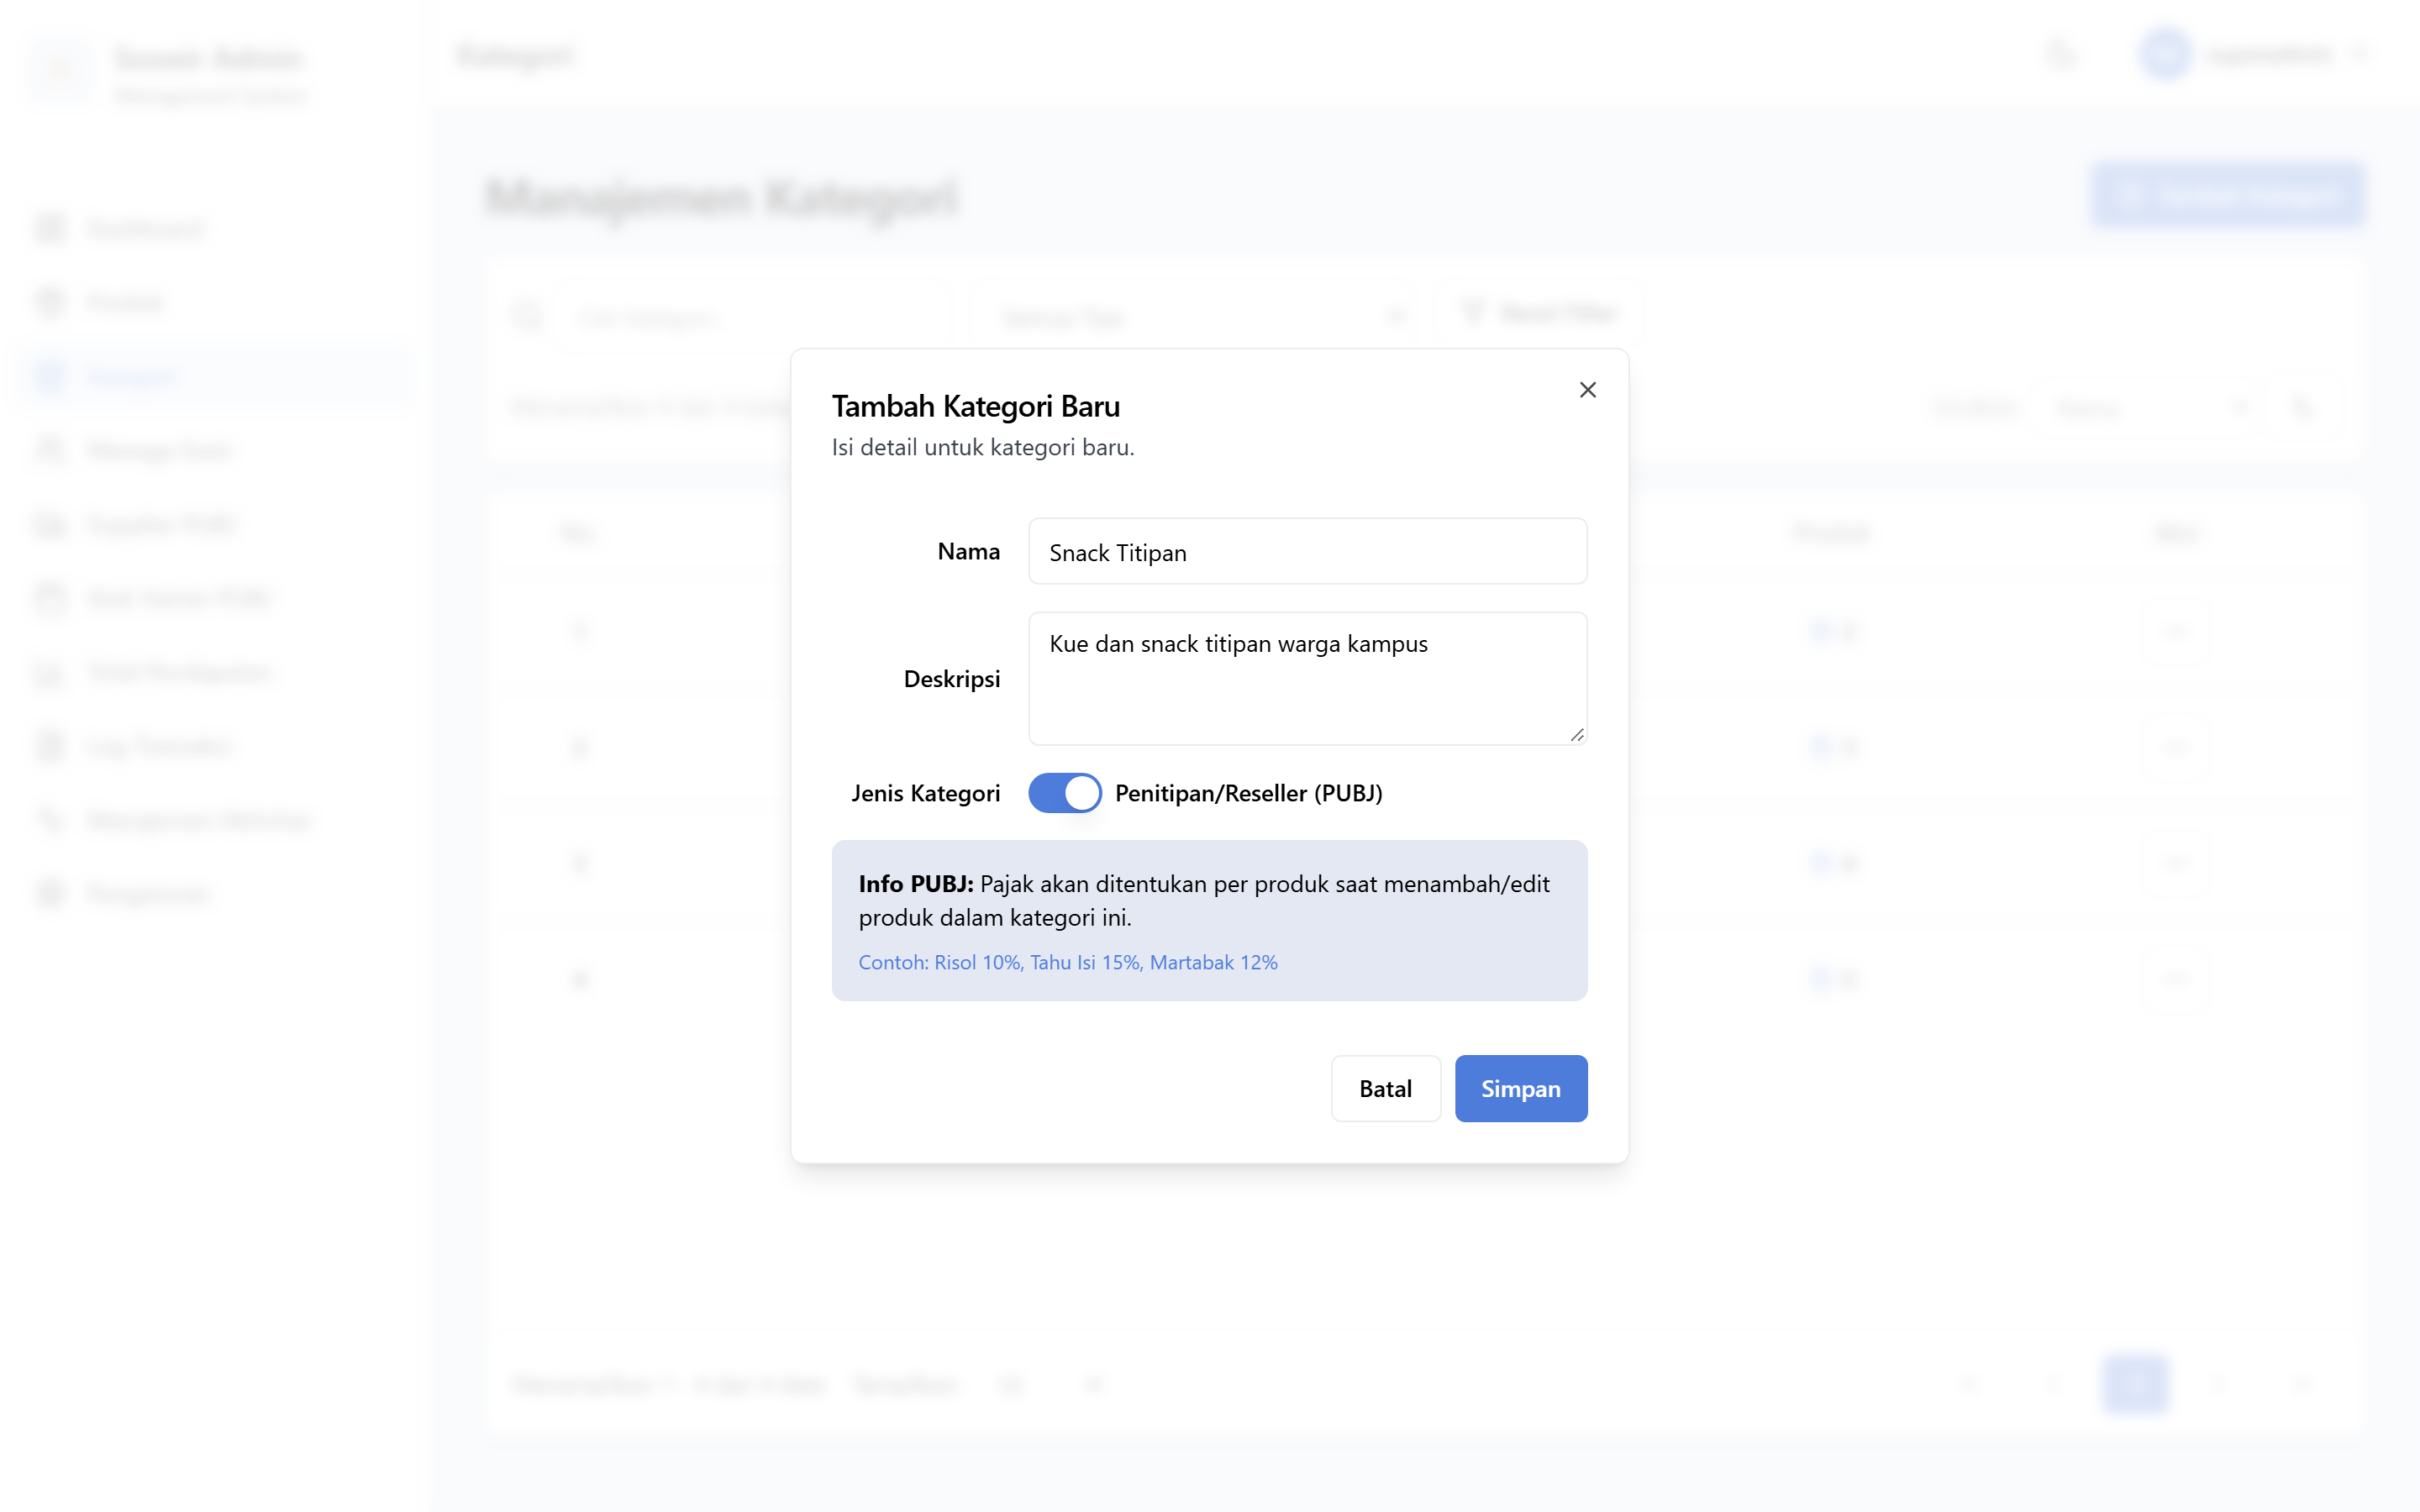
\includegraphics[width=0.99\linewidth,height=0.40\textheight,keepaspectratio,cfbox=garis 0.5pt 0pt]{img/23-kategori-tambah.png}
\caption{Jendela \ui{Tambah Kategori Baru} dengan jenis PUBJ.}
\end{figure}

\begin{catatan}
Pilihan \ui{Hapus} pada menu aksi kategori langsung menghapus tanpa jendela konfirmasi. Kategori yang masih dipakai produk tidak bisa dihapus; pindahkan dulu produknya ke kategori lain.
\end{catatan}

% ---------------------------------------------------------------
\section{Supplier PUBJ}

Menu \ui{Supplier PUBJ} menyimpan data pemilik barang titipan. Setiap produk PUBJ terhubung ke satu supplier.

\begin{figure}[H]
\centering
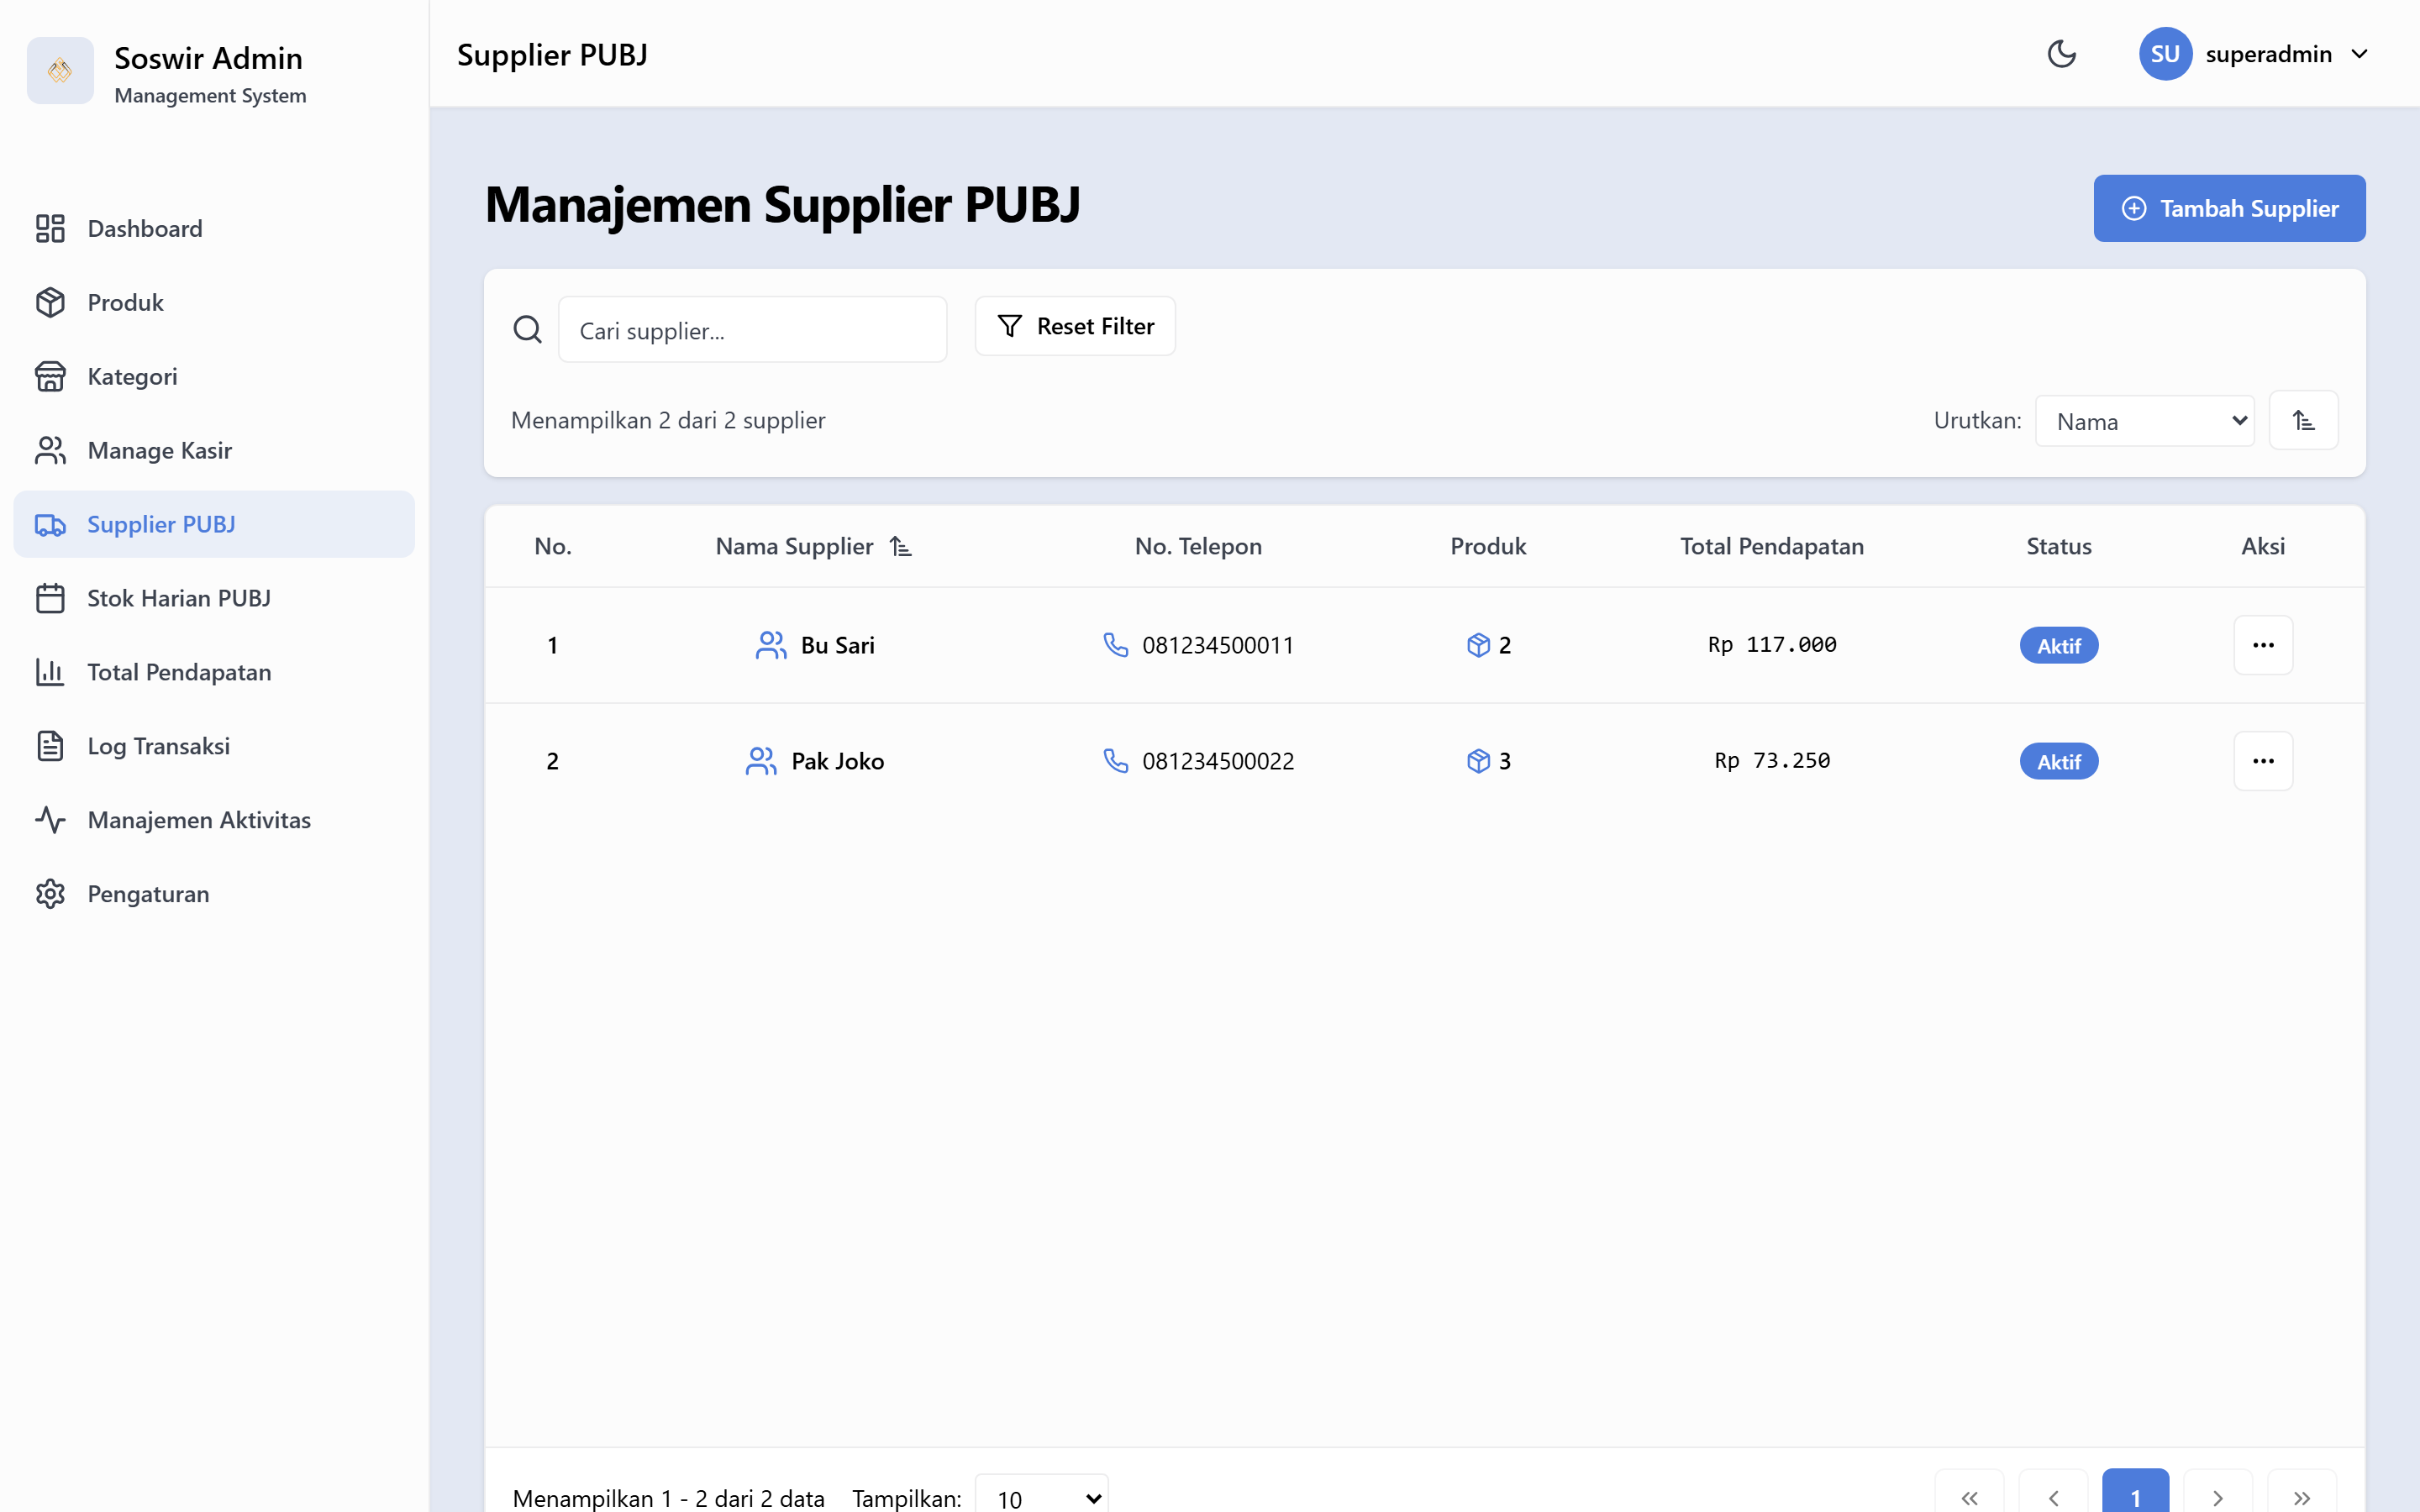
\includegraphics[width=0.99\linewidth,height=0.40\textheight,keepaspectratio,cfbox=garis 0.5pt 0pt]{img/24-supplier-daftar.png}
\caption{Halaman \ui{Manajemen Supplier PUBJ}. Kolom \ui{Total Pendapatan} adalah bagian supplier dari penjualan.}
\end{figure}

\subsection{Menambah dan mengubah supplier}

\begin{enumerate}
  \item Tekan \ui{Tambah Supplier}. Untuk mengubah, buka menu aksi supplier lalu pilih \ui{Edit}.
  \item Isi \ui{Nama Supplier}. Nama tidak boleh sama dengan supplier lain.
  \item Isi \ui{No. Telepon} bila ada.
  \item Tekan \ui{Tambah Supplier} (atau \ui{Update Supplier} saat mengubah).
\end{enumerate}

\begin{figure}[H]
\centering
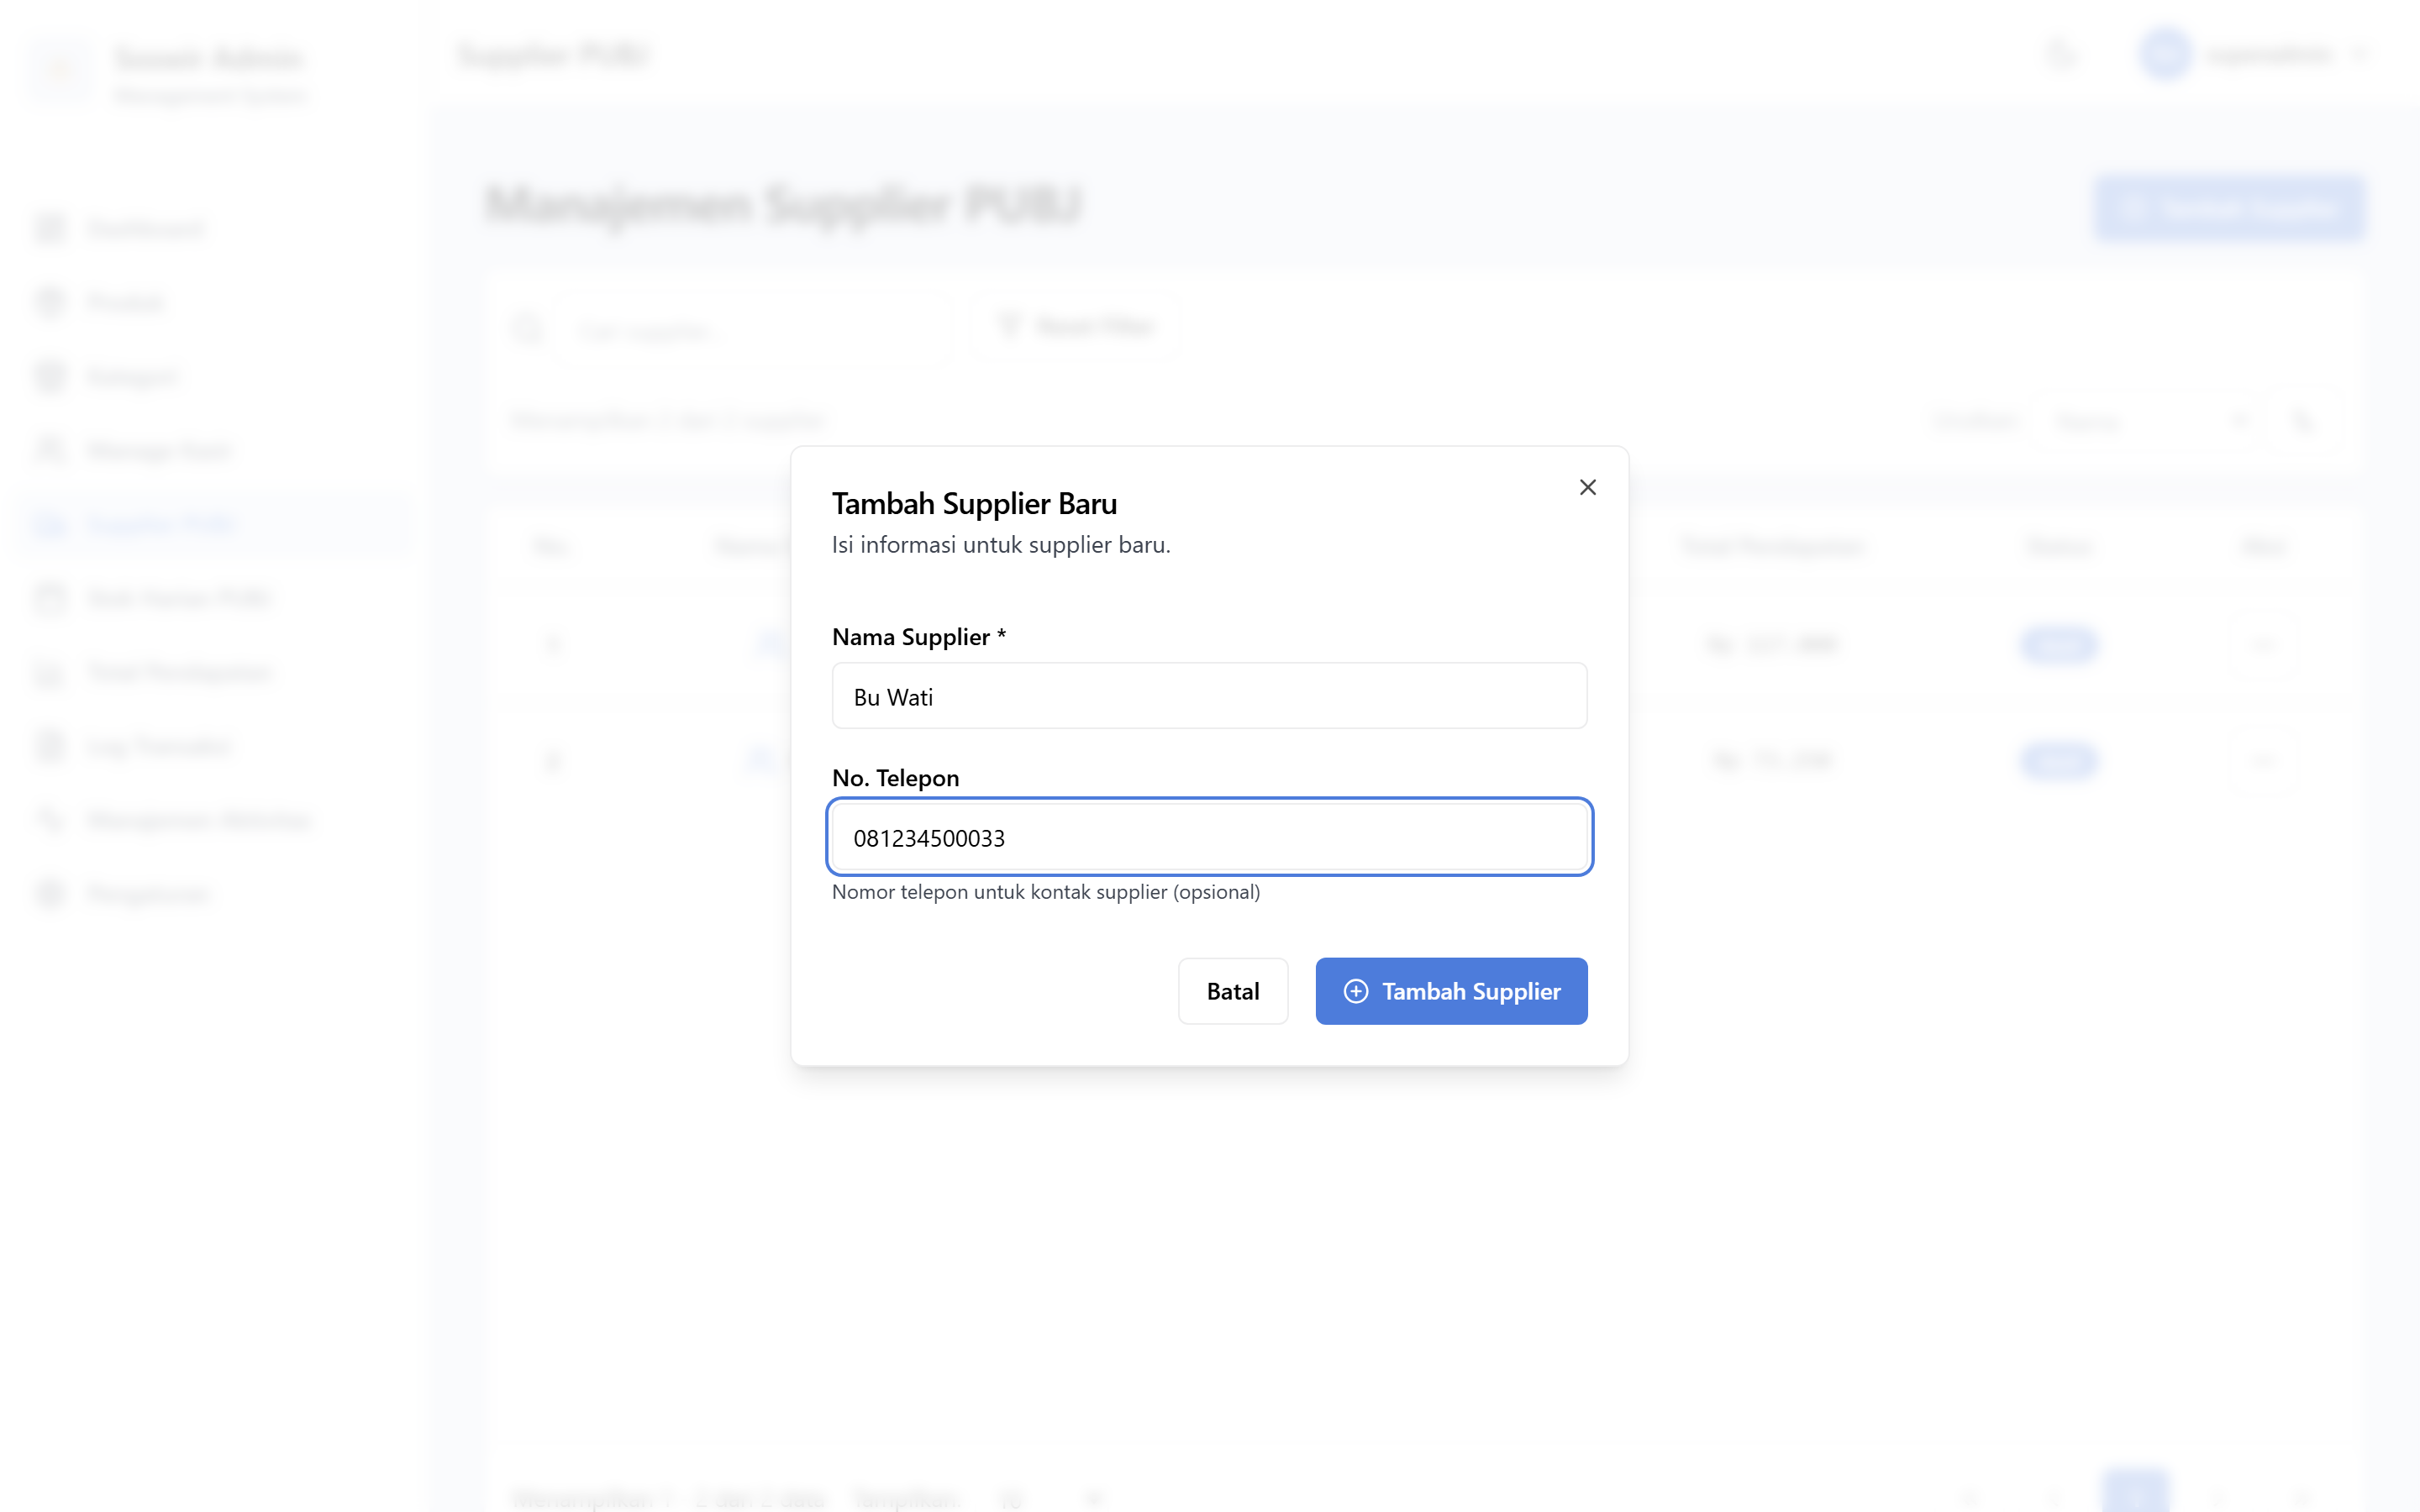
\includegraphics[width=0.99\linewidth,height=0.40\textheight,keepaspectratio,cfbox=garis 0.5pt 0pt]{img/25-supplier-tambah.png}
\caption{Jendela \ui{Tambah Supplier Baru}.}
\end{figure}

Pilihan \ui{Hapus} pada menu aksi meminta konfirmasi dulu. Data yang terkait dengan supplier itu akan dinonaktifkan.

\subsection{Melihat riwayat supplier}

\begin{enumerate}
  \item Buka menu aksi supplier, pilih \ui{Lihat Riwayat}.
  \item Jendela \ui{Riwayat Stok} menampilkan \ui{Rangkuman Historis}, \ui{Estimasi Total Pendapatan Supplier}, \ui{Estimasi Fee Toko}, dan tabel stok masuk per tanggal.
  \item Tekan \ui{Tutup} setelah selesai.
\end{enumerate}

\begin{figure}[H]
\centering
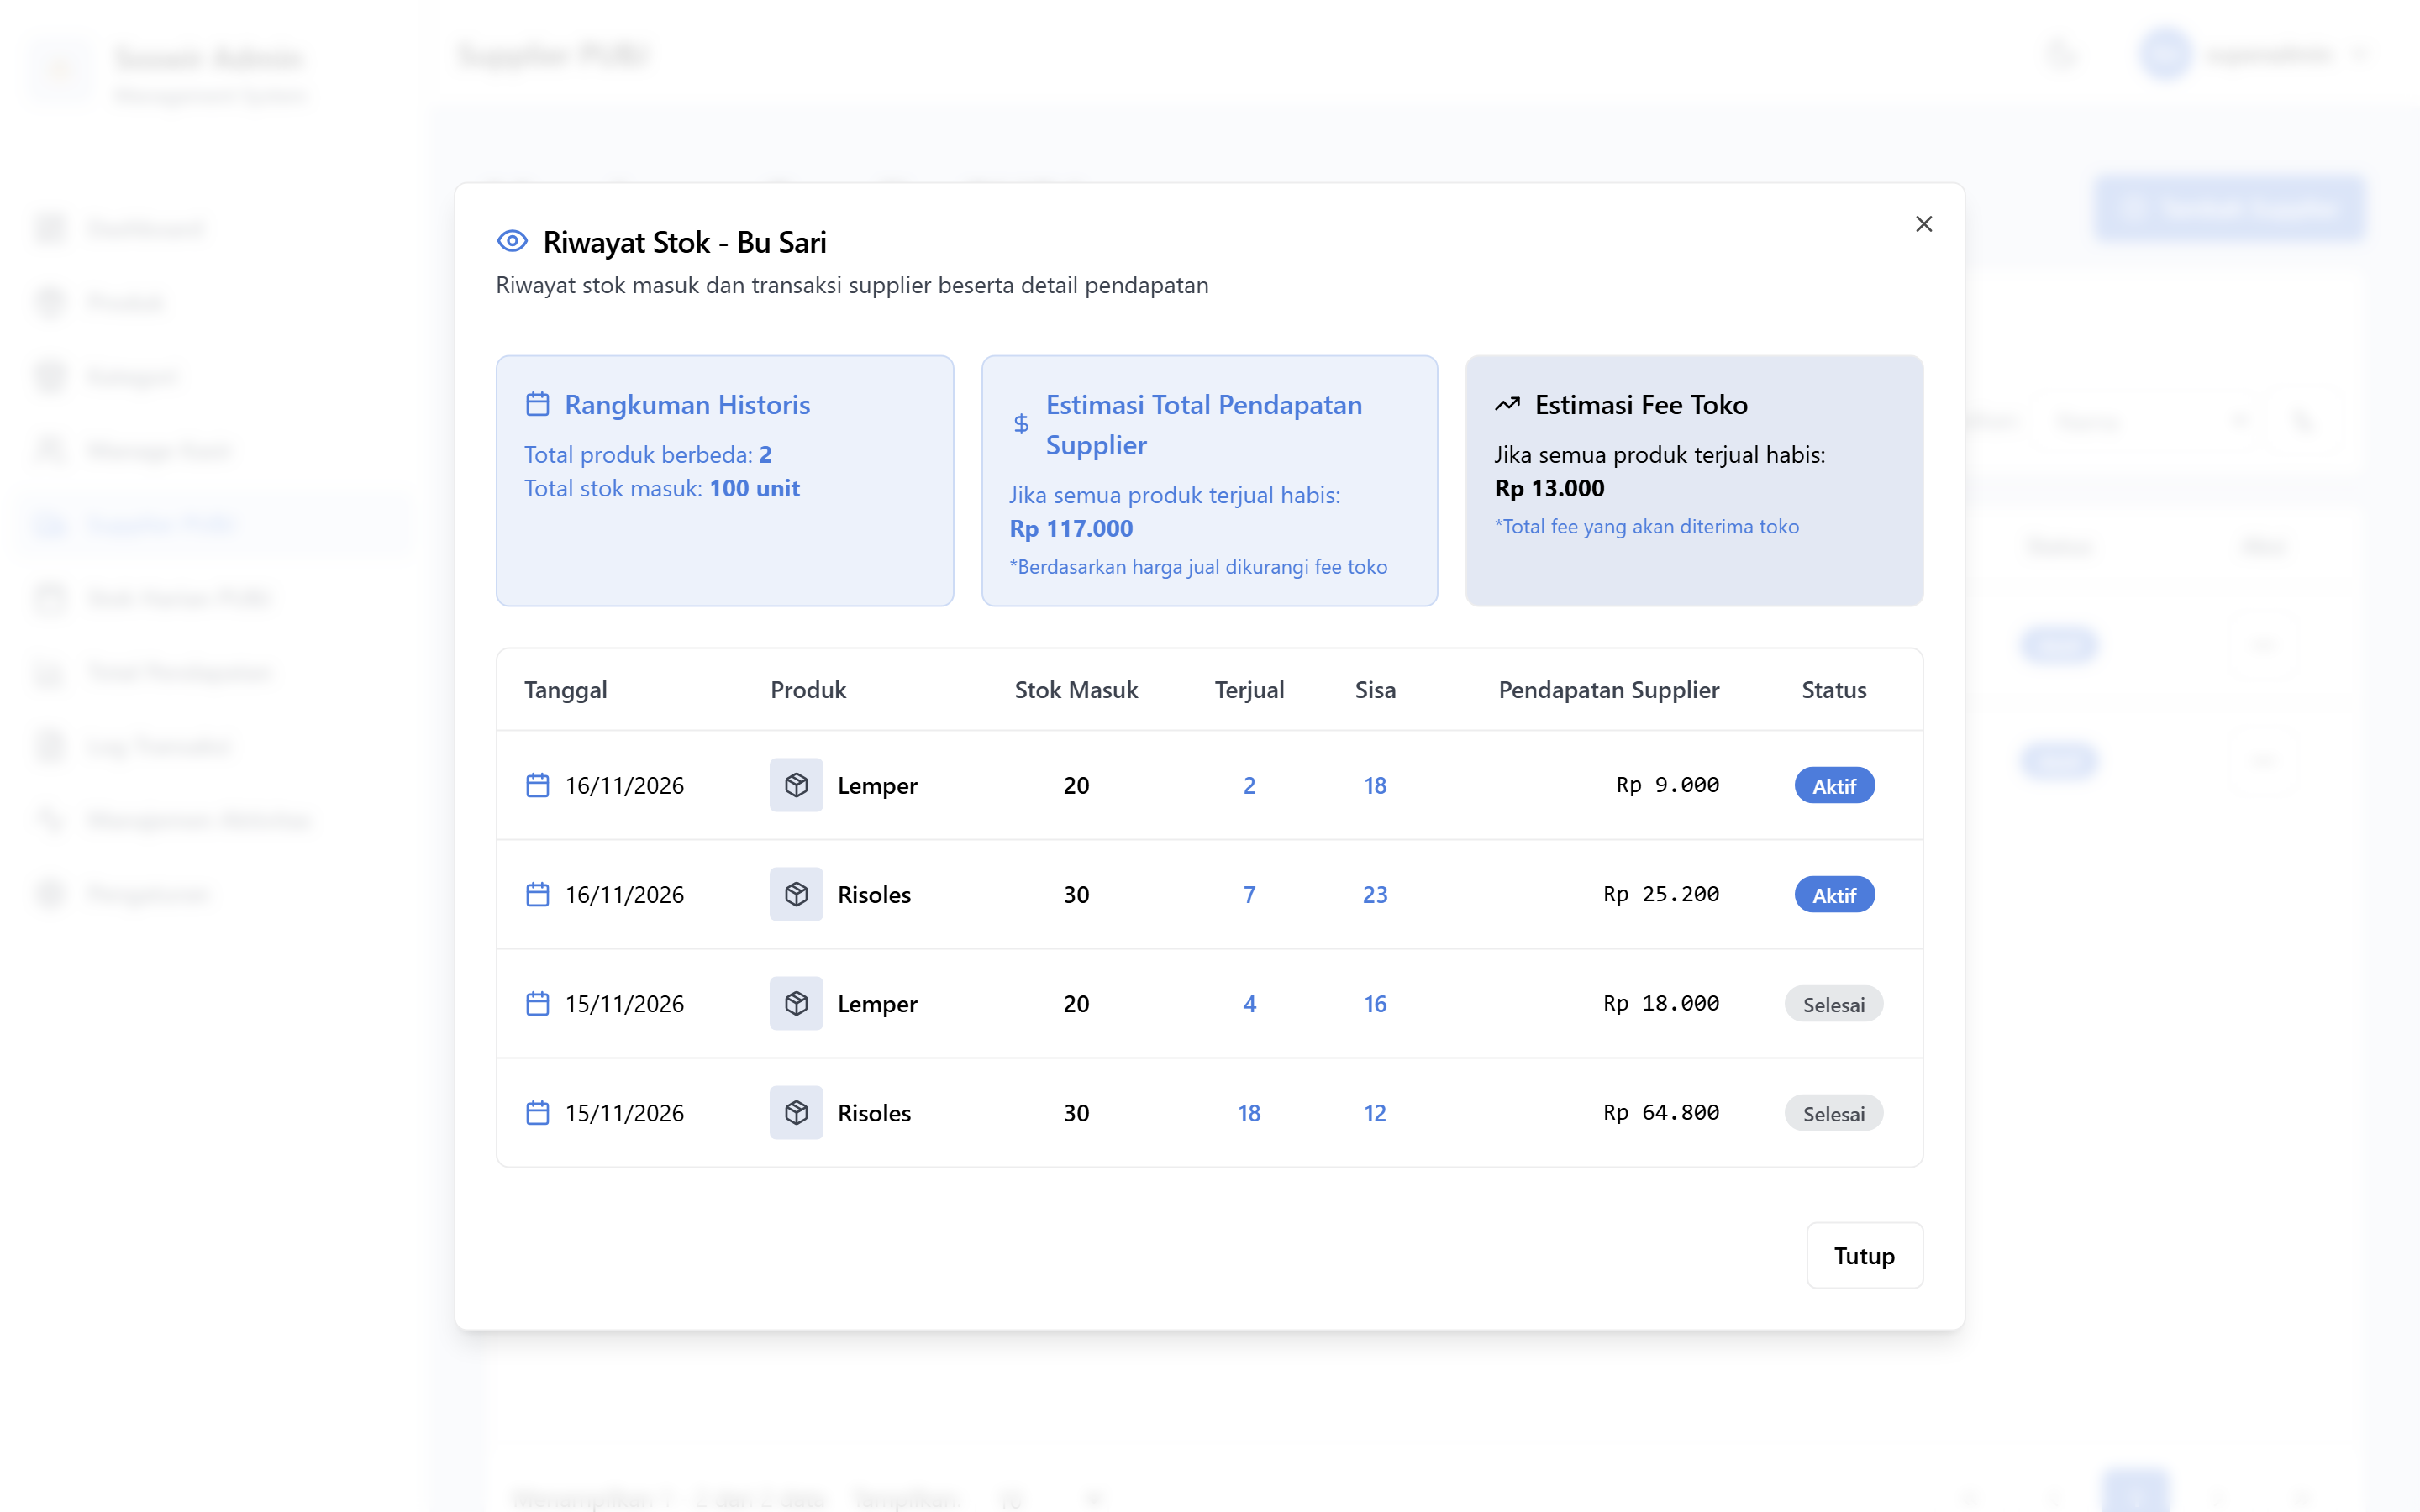
\includegraphics[width=0.99\linewidth,height=0.40\textheight,keepaspectratio,cfbox=garis 0.5pt 0pt]{img/26-supplier-riwayat.png}
\caption{Riwayat stok titipan Bu Sari.}
\end{figure}

Angka estimasi dihitung dengan anggapan semua barang terjual habis. Pendapatan yang benar-benar terjadi ada di kolom \ui{Pendapatan Supplier}.

% ---------------------------------------------------------------
\section{Stok Harian PUBJ}
\label{sec:stokharian}

Barang titipan datang setiap hari, jadi stoknya dicatat per hari. Satu catatan (entry) berisi satu produk dari satu supplier pada satu tanggal.

\begin{figure}[H]
\centering
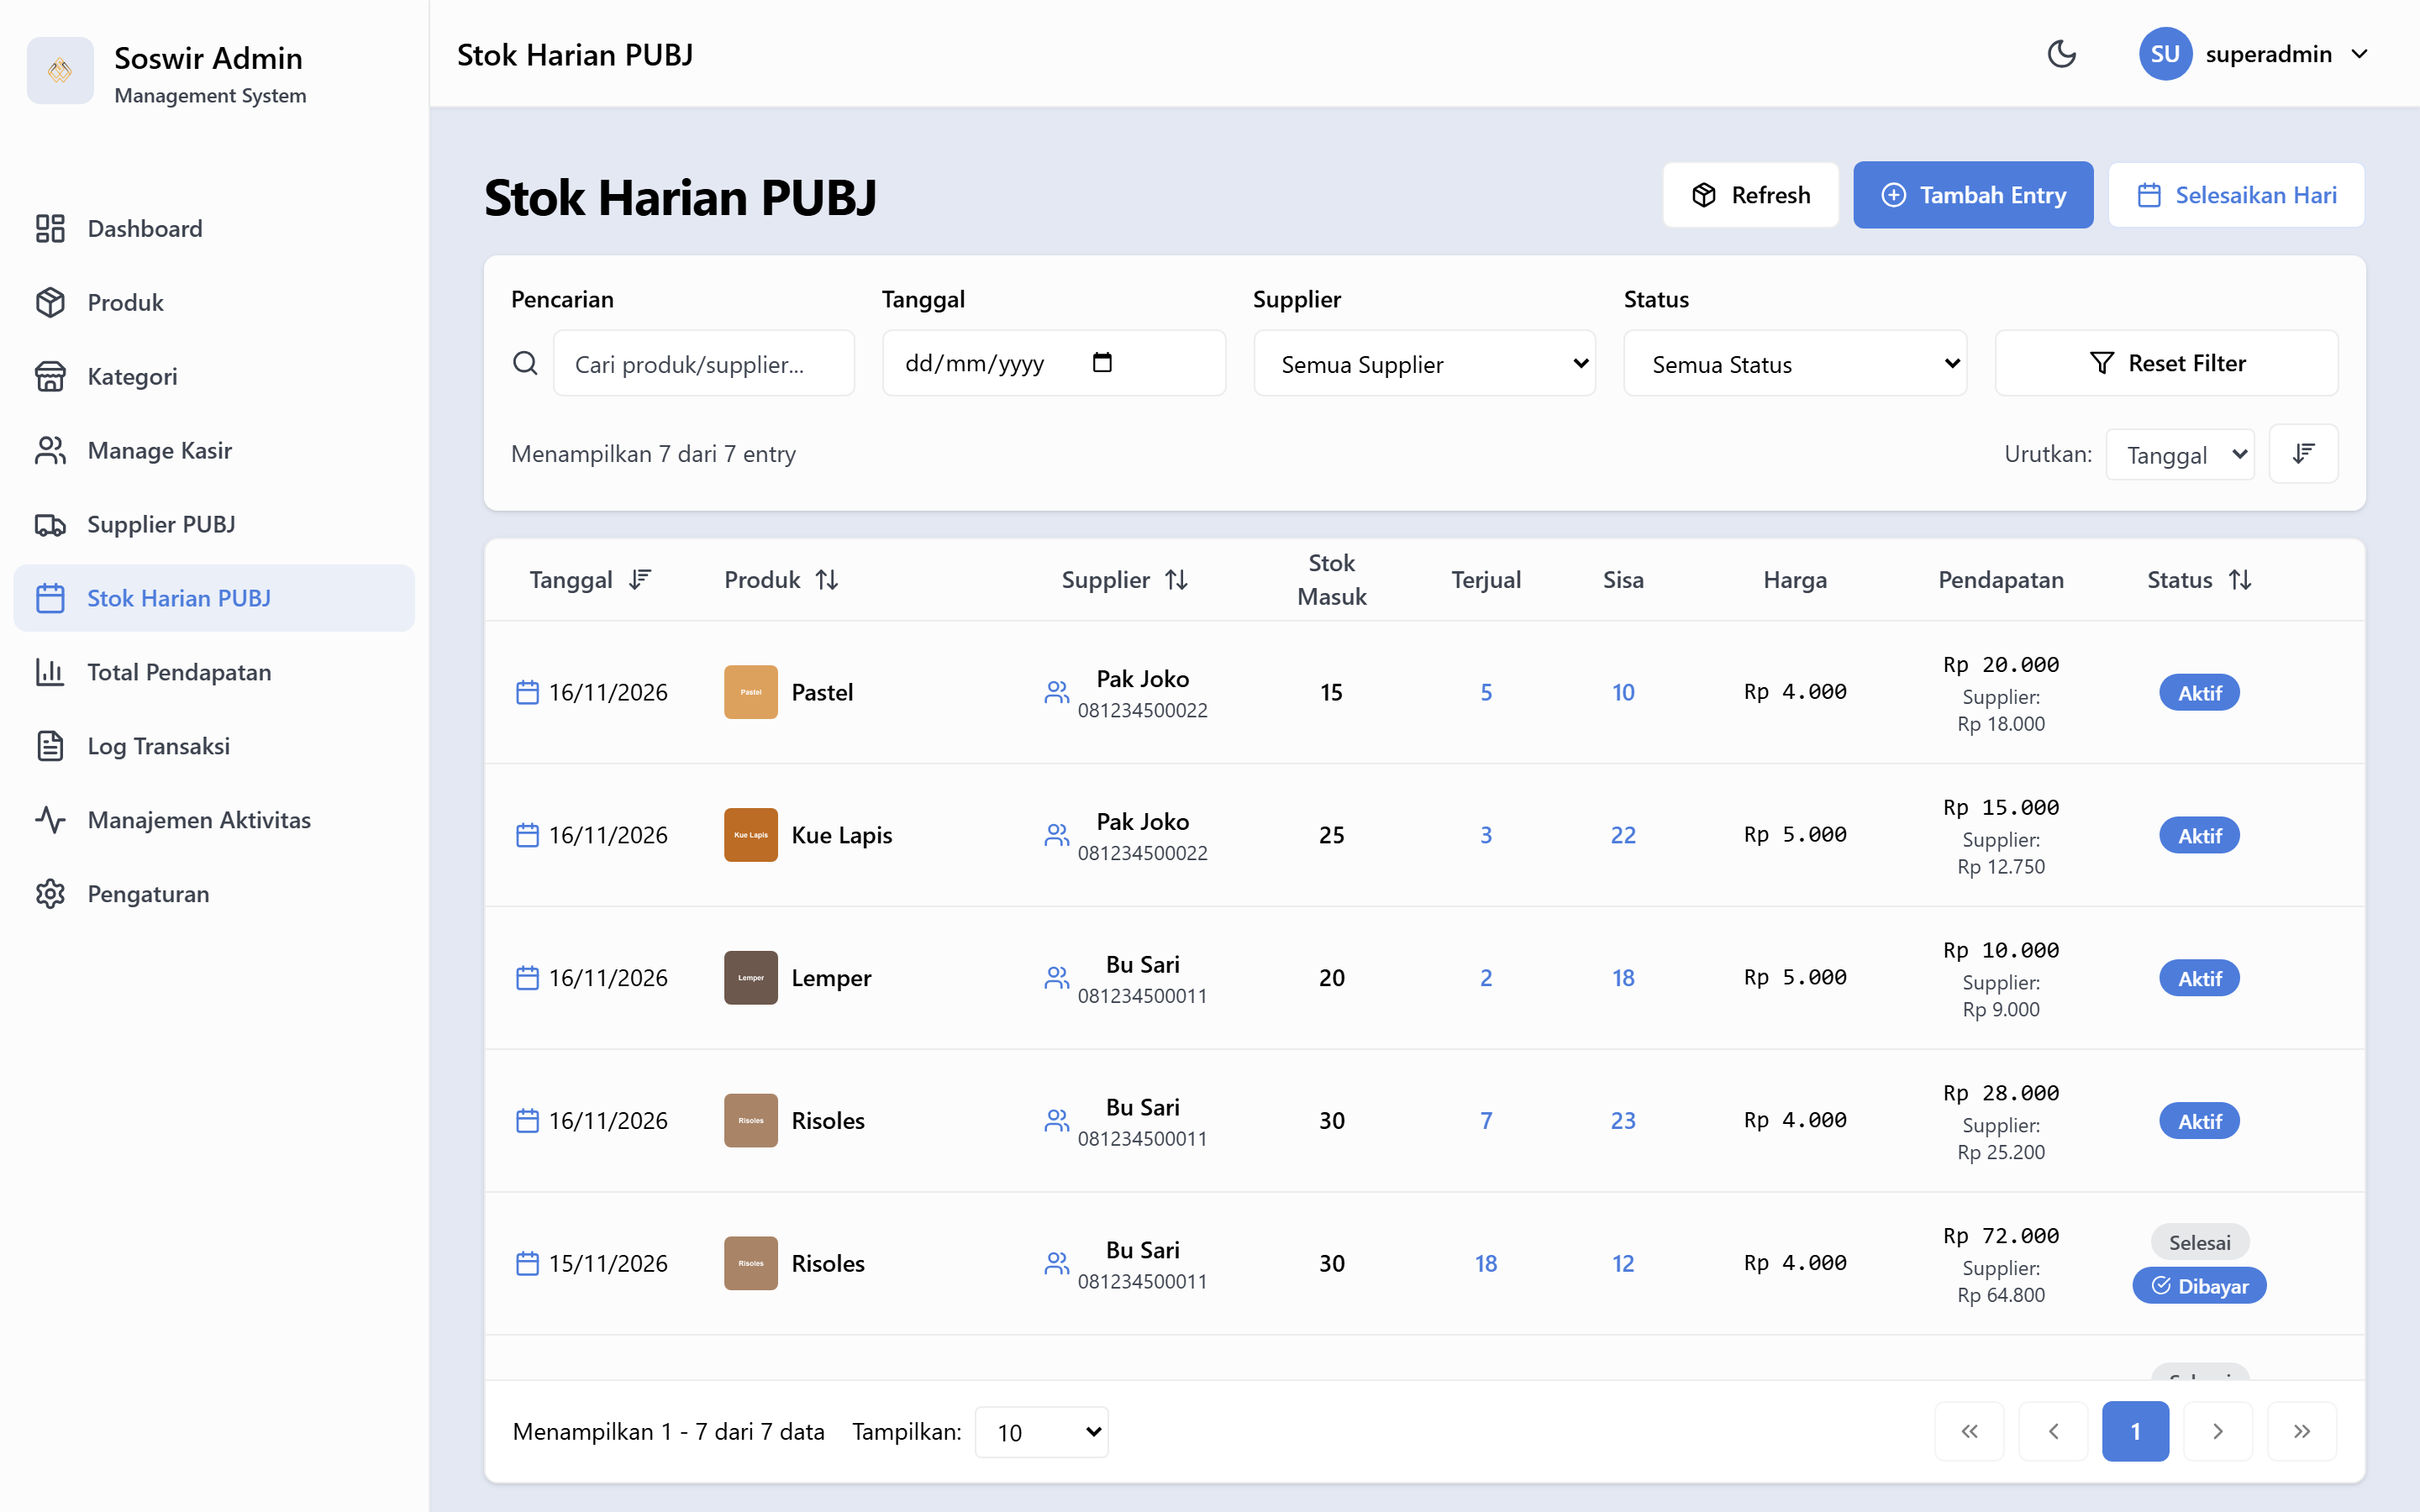
\includegraphics[width=0.99\linewidth,height=0.40\textheight,keepaspectratio,cfbox=garis 0.5pt 0pt]{img/27-stok-harian-daftar.png}
\caption{Halaman \ui{Stok Harian PUBJ}.}
\end{figure}

Arti kolom tabel:

\begin{itemize}
  \item \ui{Stok Masuk}: jumlah barang yang dititipkan hari itu.
  \item \ui{Terjual} dan \ui{Sisa}: barang yang sudah laku dan yang belum.
  \item \ui{Pendapatan}: hasil penjualan, dengan bagian \ui{Supplier} di bawahnya.
  \item \ui{Status}: \ui{Aktif} berarti masih bisa dijual; \ui{Selesai} berarti sudah ditutup. Entry yang selesai juga bertanda \ui{Belum Bayar} atau \ui{Dibayar}.
\end{itemize}

\begin{catatan}
Kasir hanya bisa menjual produk PUBJ yang punya entry \ui{Aktif} untuk hari ini. Setiap hari pukul 18:00 WIB, semua entry yang masih aktif ditutup otomatis menjadi \ui{Selesai}, dan sisa barangnya dianggap dikembalikan ke supplier. Besok pagi, catat stok masuk yang baru.
\end{catatan}

\subsection{Mencatat stok masuk hari ini}

\begin{enumerate}
  \item Tekan \ui{Tambah Entry}.
  \item \ui{Tanggal} terisi hari ini. Pilih \ui{Supplier}, lalu \ui{Produk} milik supplier tersebut.
  \item Isi \ui{Jumlah Stok Masuk} dengan bilangan bulat lebih dari 0. \ui{Catatan} boleh diisi.
  \item Tekan \ui{Simpan Entry}. Stok produk di kasir langsung bertambah.
\end{enumerate}

\begin{figure}[H]
\centering
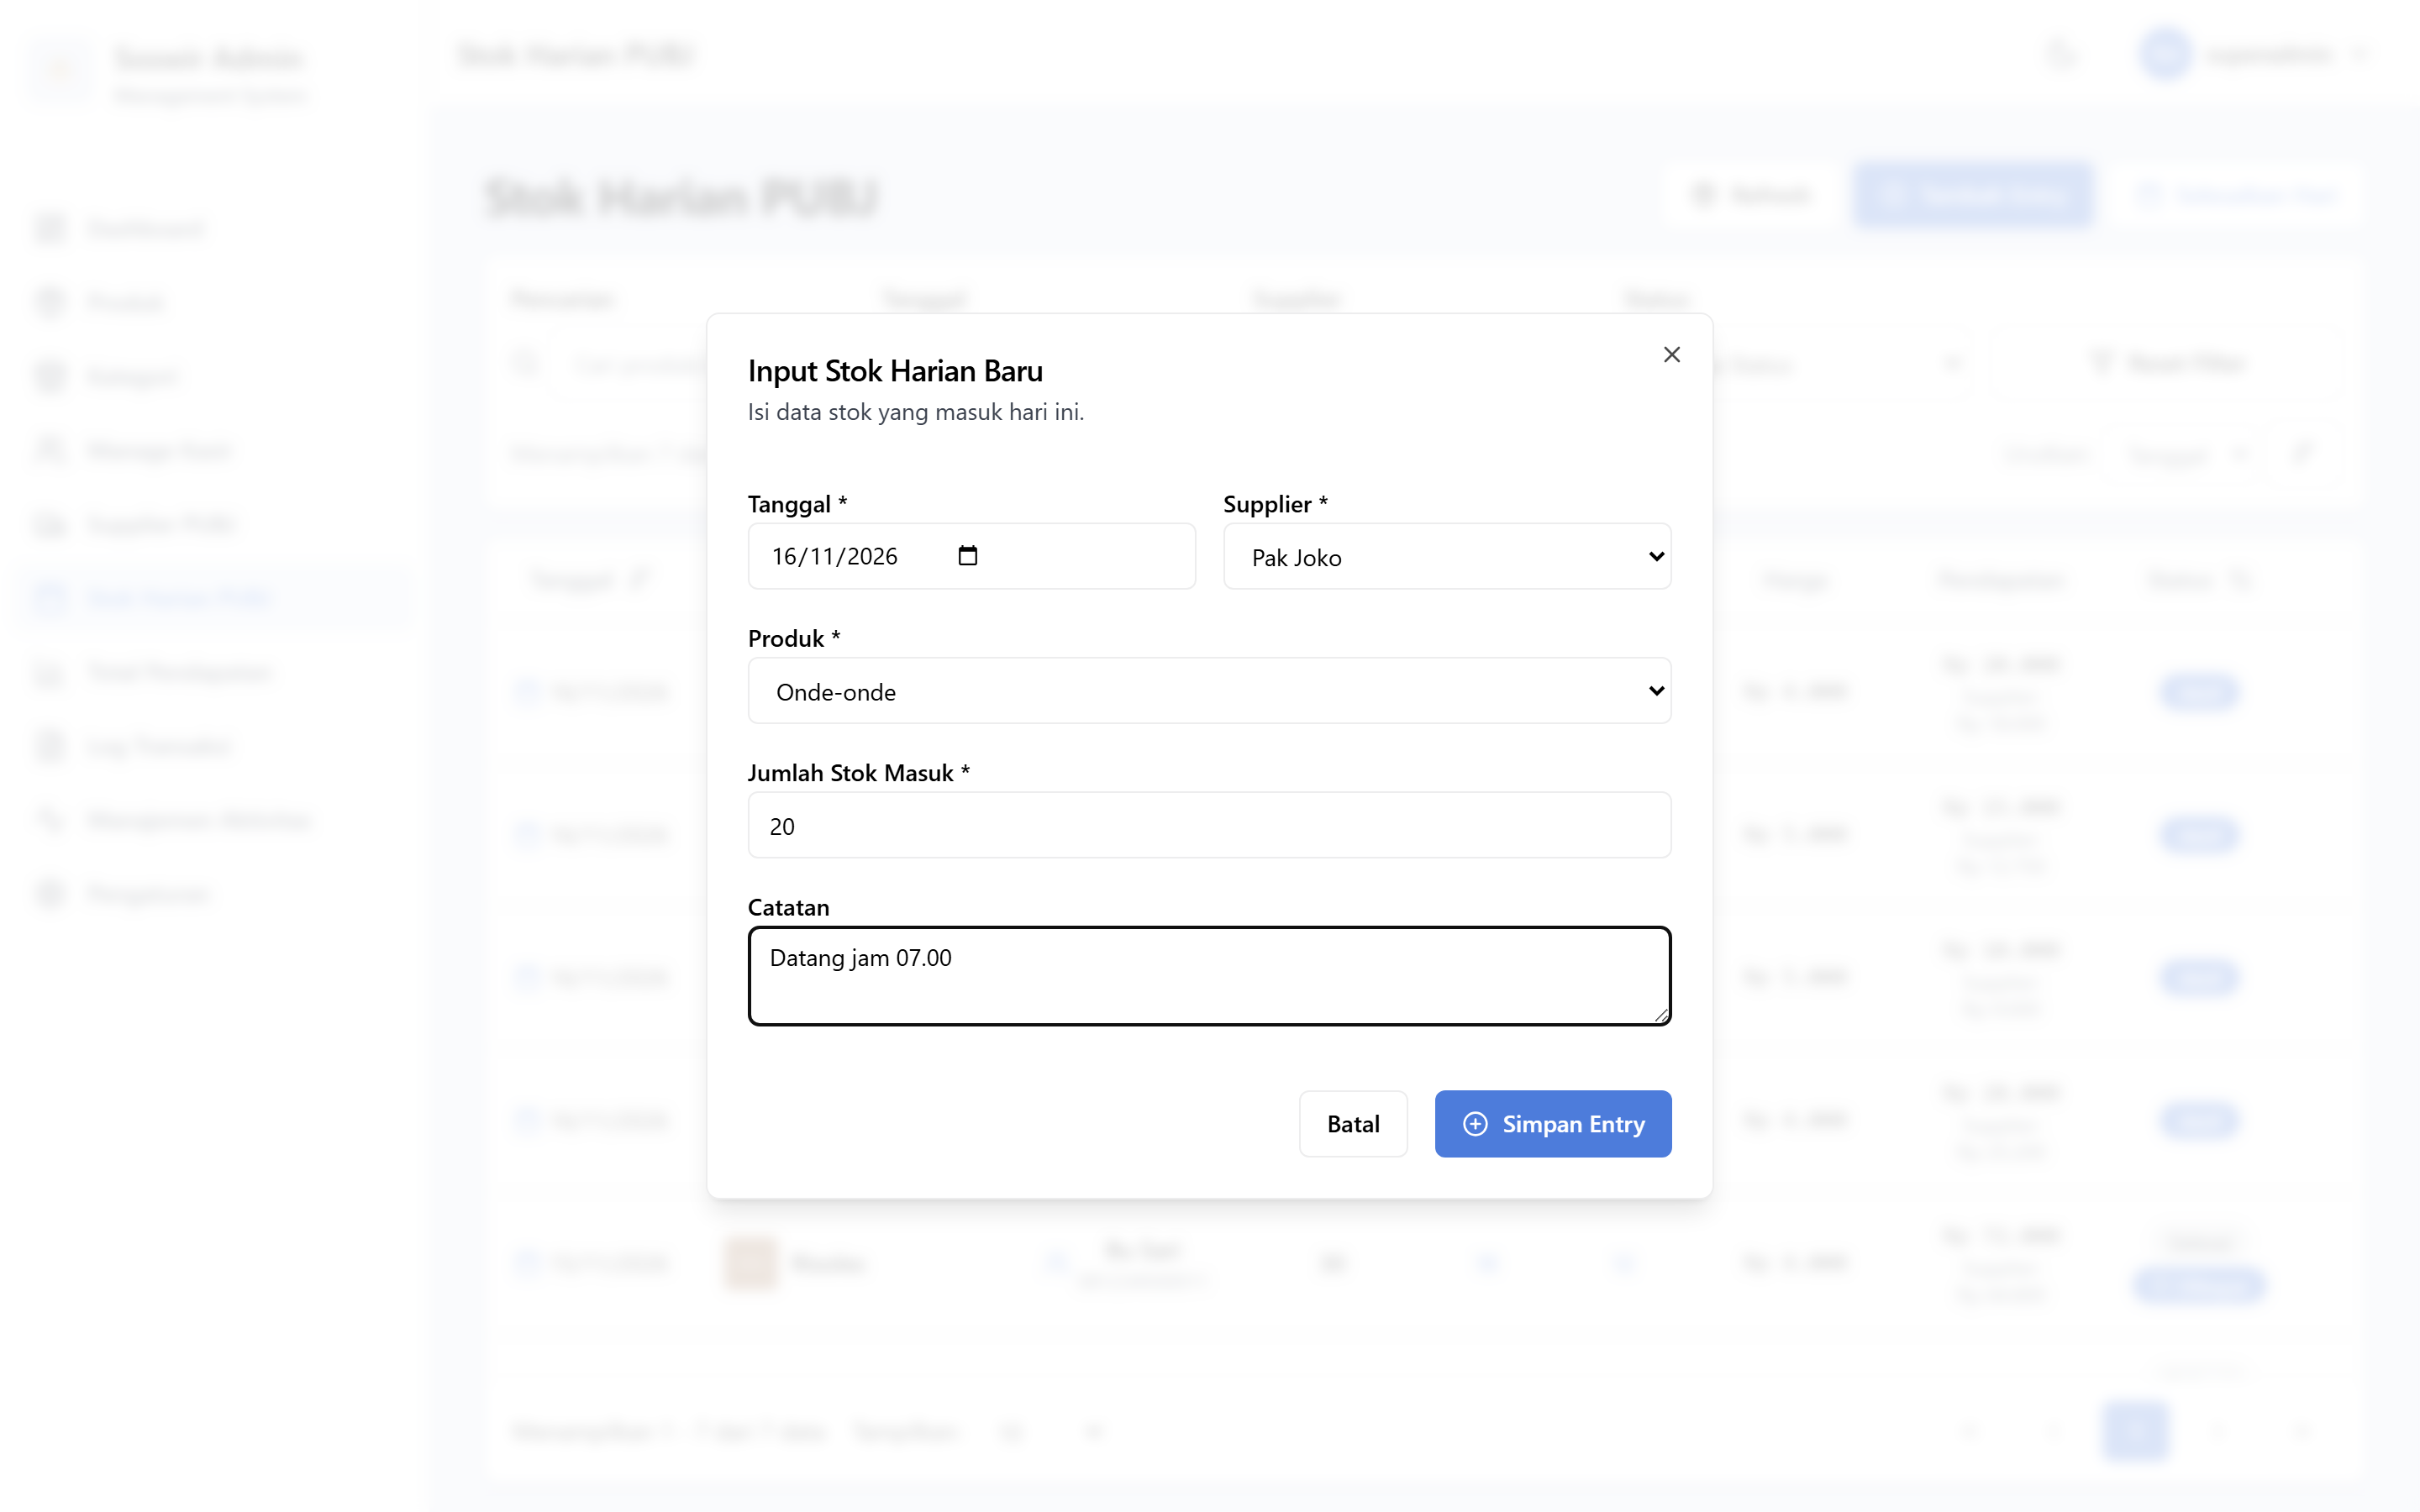
\includegraphics[width=0.99\linewidth,height=0.40\textheight,keepaspectratio,cfbox=garis 0.5pt 0pt]{img/28-stok-harian-tambah.png}
\caption{Jendela \ui{Input Stok Harian Baru}.}
\end{figure}

Satu produk dari supplier yang sama hanya boleh punya satu entry per tanggal. Kalau ada tambahan barang di hari yang sama, ubah entry yang sudah ada.

\subsection{Mengubah jumlah stok masuk}

\begin{enumerate}
  \item Buka menu aksi entry yang masih \ui{Aktif}, pilih \ui{Edit}.
  \item Ubah \ui{Jumlah Stok Masuk}. Jumlah ini tidak boleh lebih kecil dari barang yang sudah terjual.
  \item Tekan \ui{Update Entry}.
\end{enumerate}

\begin{figure}[H]
\centering
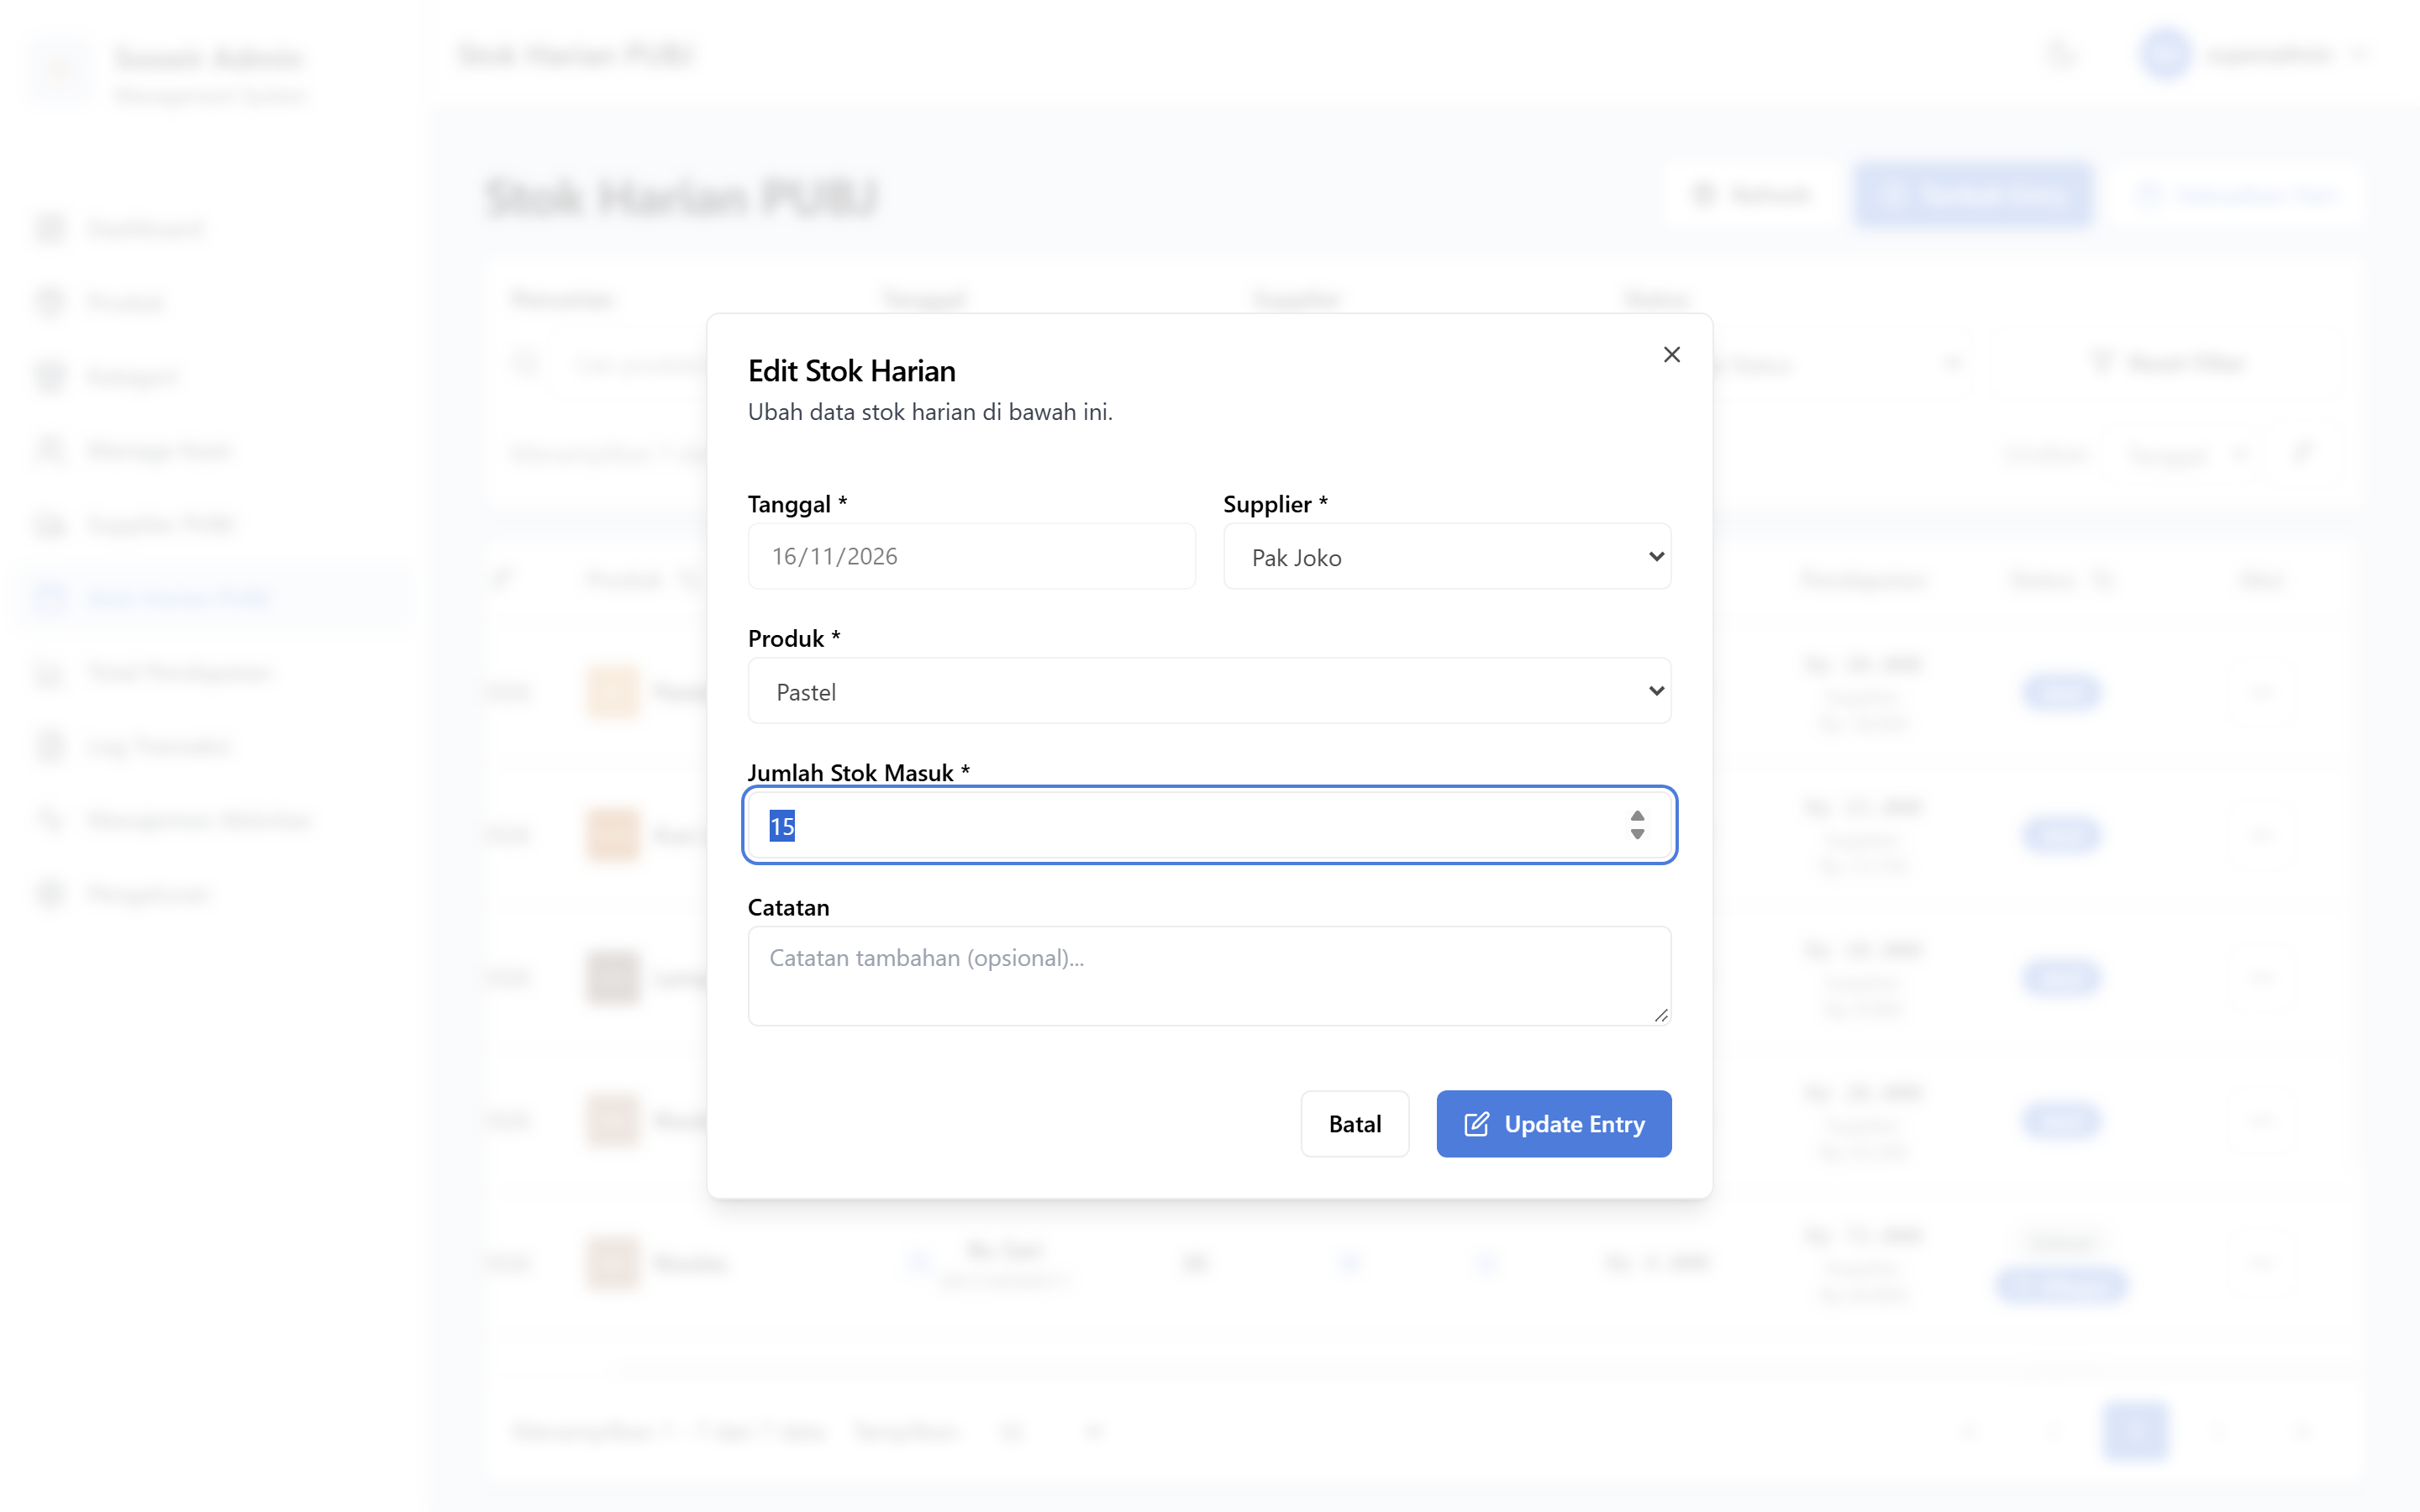
\includegraphics[width=0.99\linewidth,height=0.40\textheight,keepaspectratio,cfbox=garis 0.5pt 0pt]{img/29-stok-harian-edit.png}
\caption{Jendela \ui{Edit Stok Harian}. Tanggal, supplier, dan produk tidak bisa diganti.}
\end{figure}

\subsection{Menyelesaikan satu entry}

Pakai ini kalau sisa barang satu produk diambil kembali oleh supplier sebelum pukul 18:00.

\begin{enumerate}
  \item Buka menu aksi entry, pilih \ui{Selesaikan}.
  \item Periksa \ui{Stok Masuk}, \ui{Terjual}, dan \ui{Sisa} di jendela \ui{Selesaikan Stok Harian}.
  \item Tekan \ui{Selesaikan}. Produk itu tidak bisa dijual lagi hari ini.
\end{enumerate}

\begin{figure}[H]
\centering
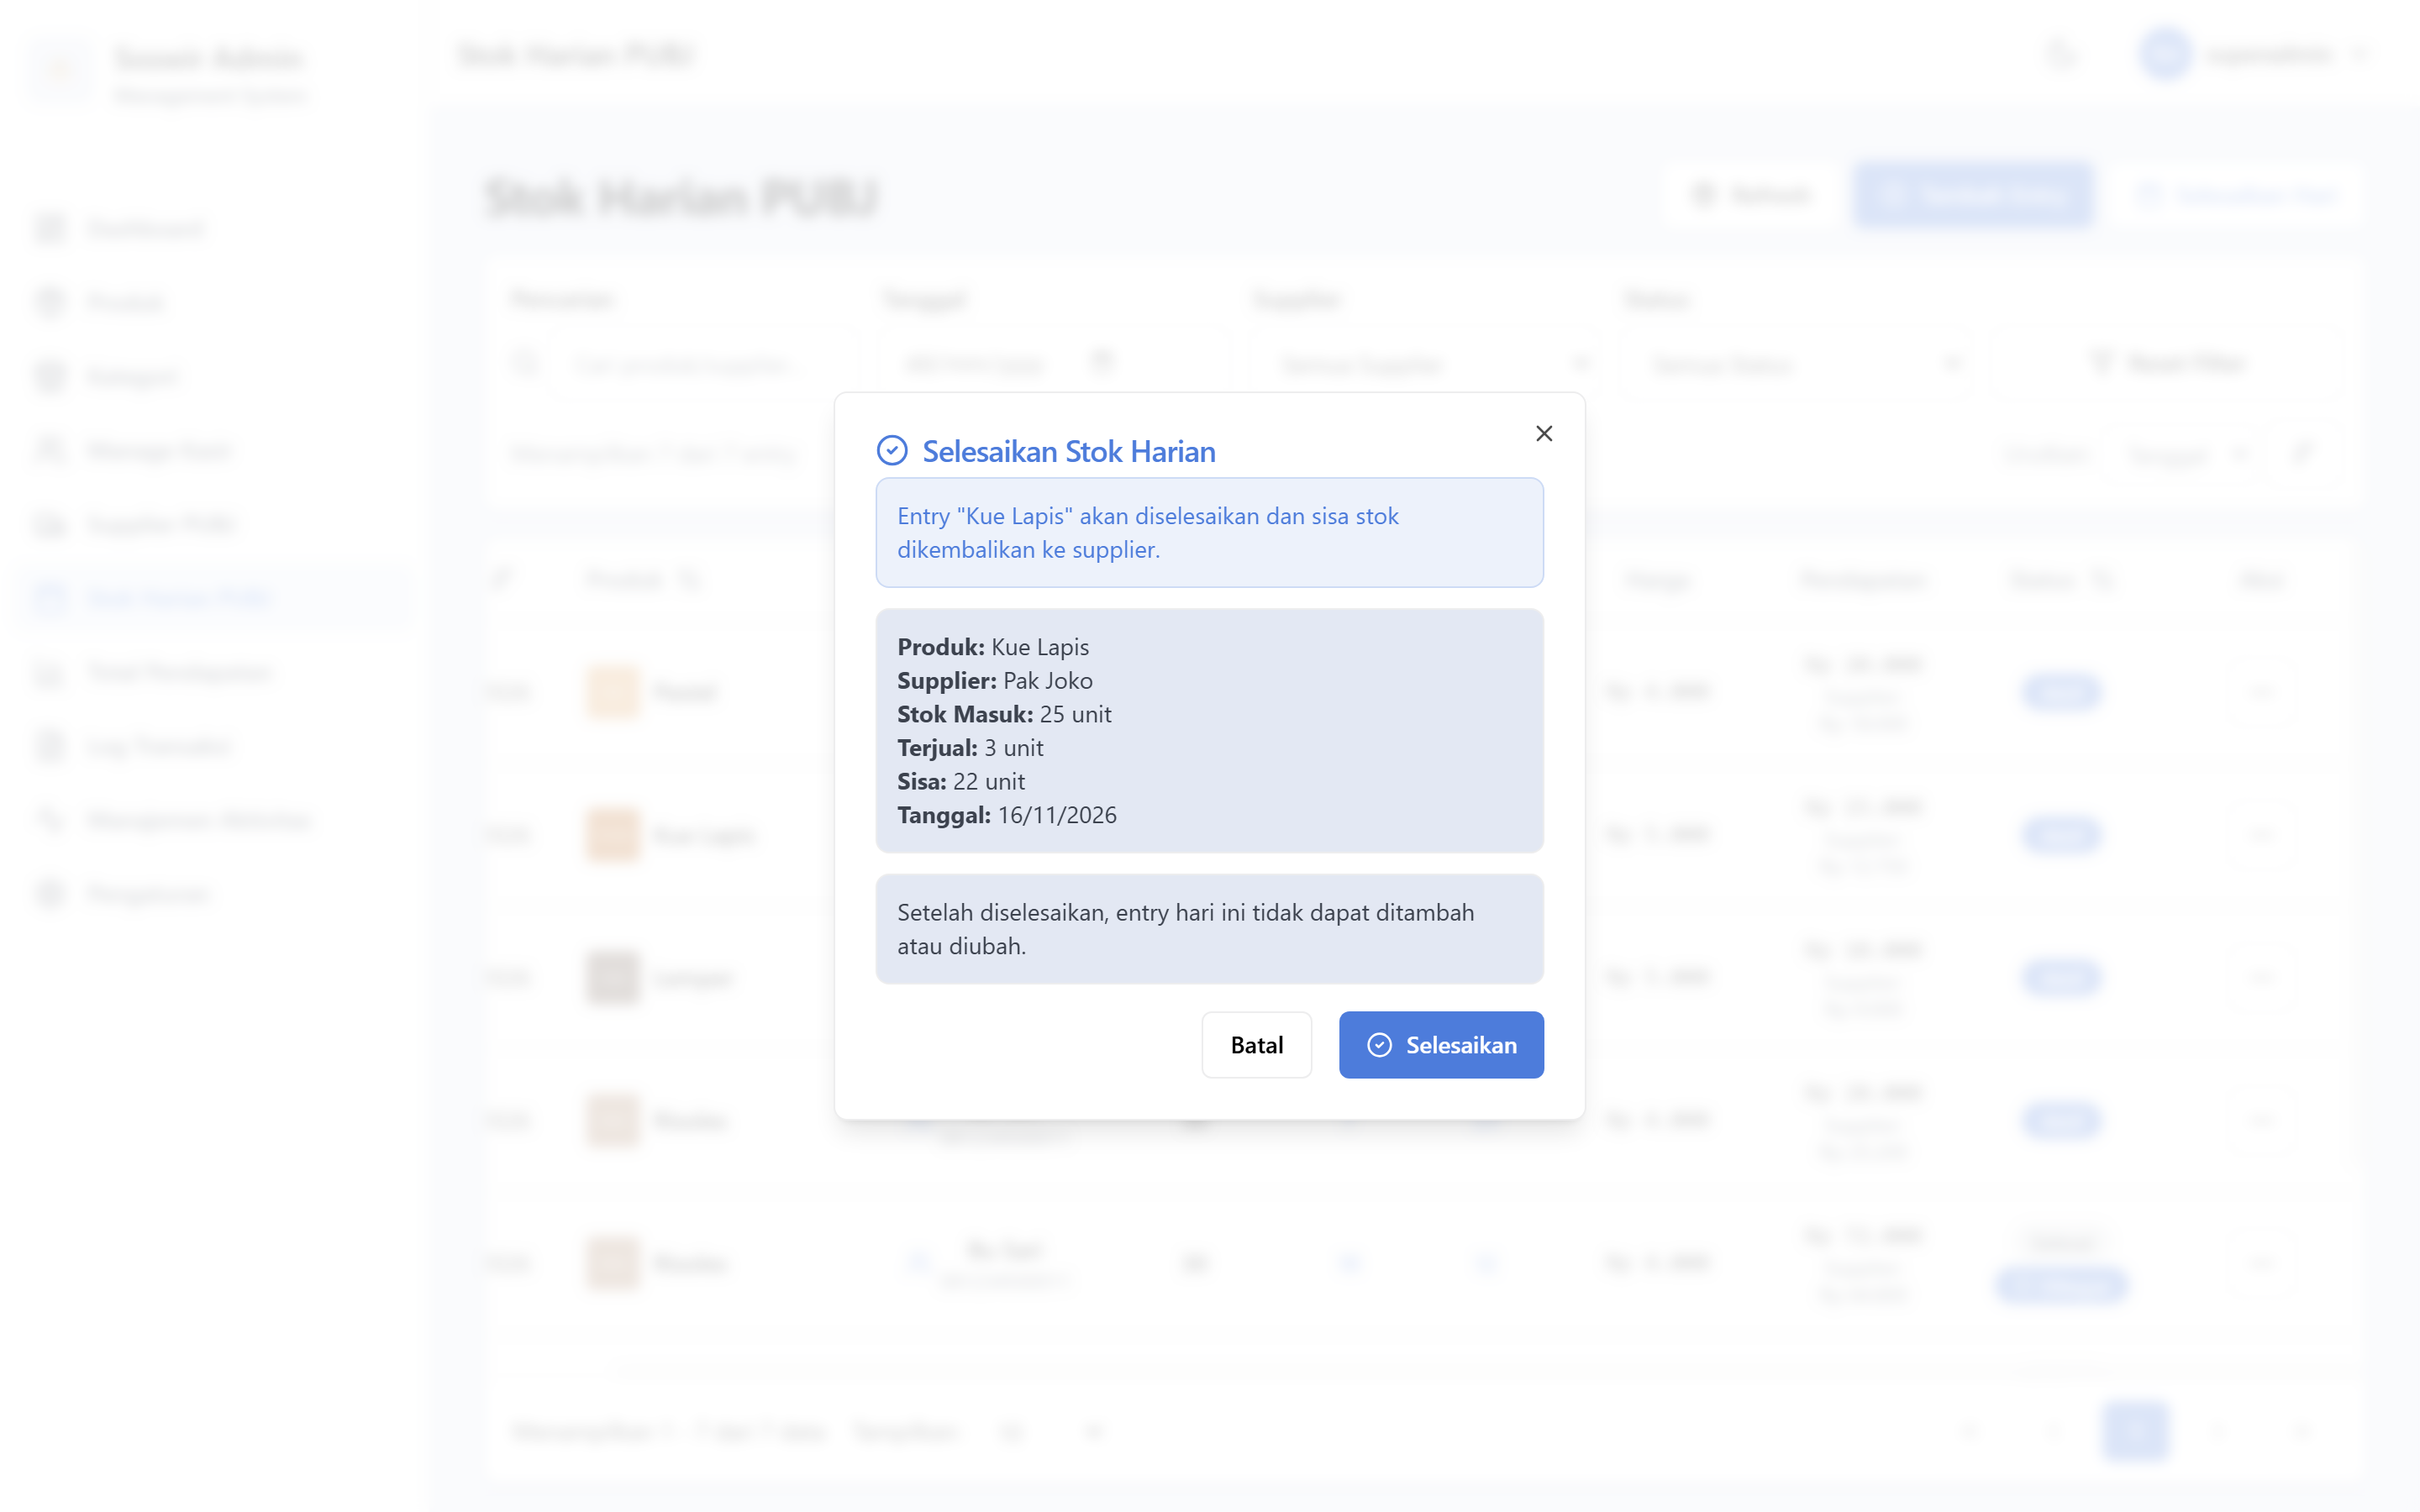
\includegraphics[width=0.99\linewidth,height=0.40\textheight,keepaspectratio,cfbox=garis 0.5pt 0pt]{img/30-stok-harian-selesaikan.png}
\caption{Konfirmasi menyelesaikan satu entry.}
\end{figure}

\subsection{Menutup semua entry hari ini}

Tombol \ui{Selesaikan Hari} menutup semua entry aktif sekaligus, misalnya saat toko tutup lebih awal dari pukul 18:00.

\begin{enumerate}
  \item Tekan \ui{Selesaikan Hari} di kanan atas.
  \item Periksa \ui{Total Entry}, \ui{Total Produk}, dan \ui{Total Stok Ditambahkan}.
  \item Tekan \ui{Selesaikan Semua}.
\end{enumerate}

\begin{figure}[H]
\centering
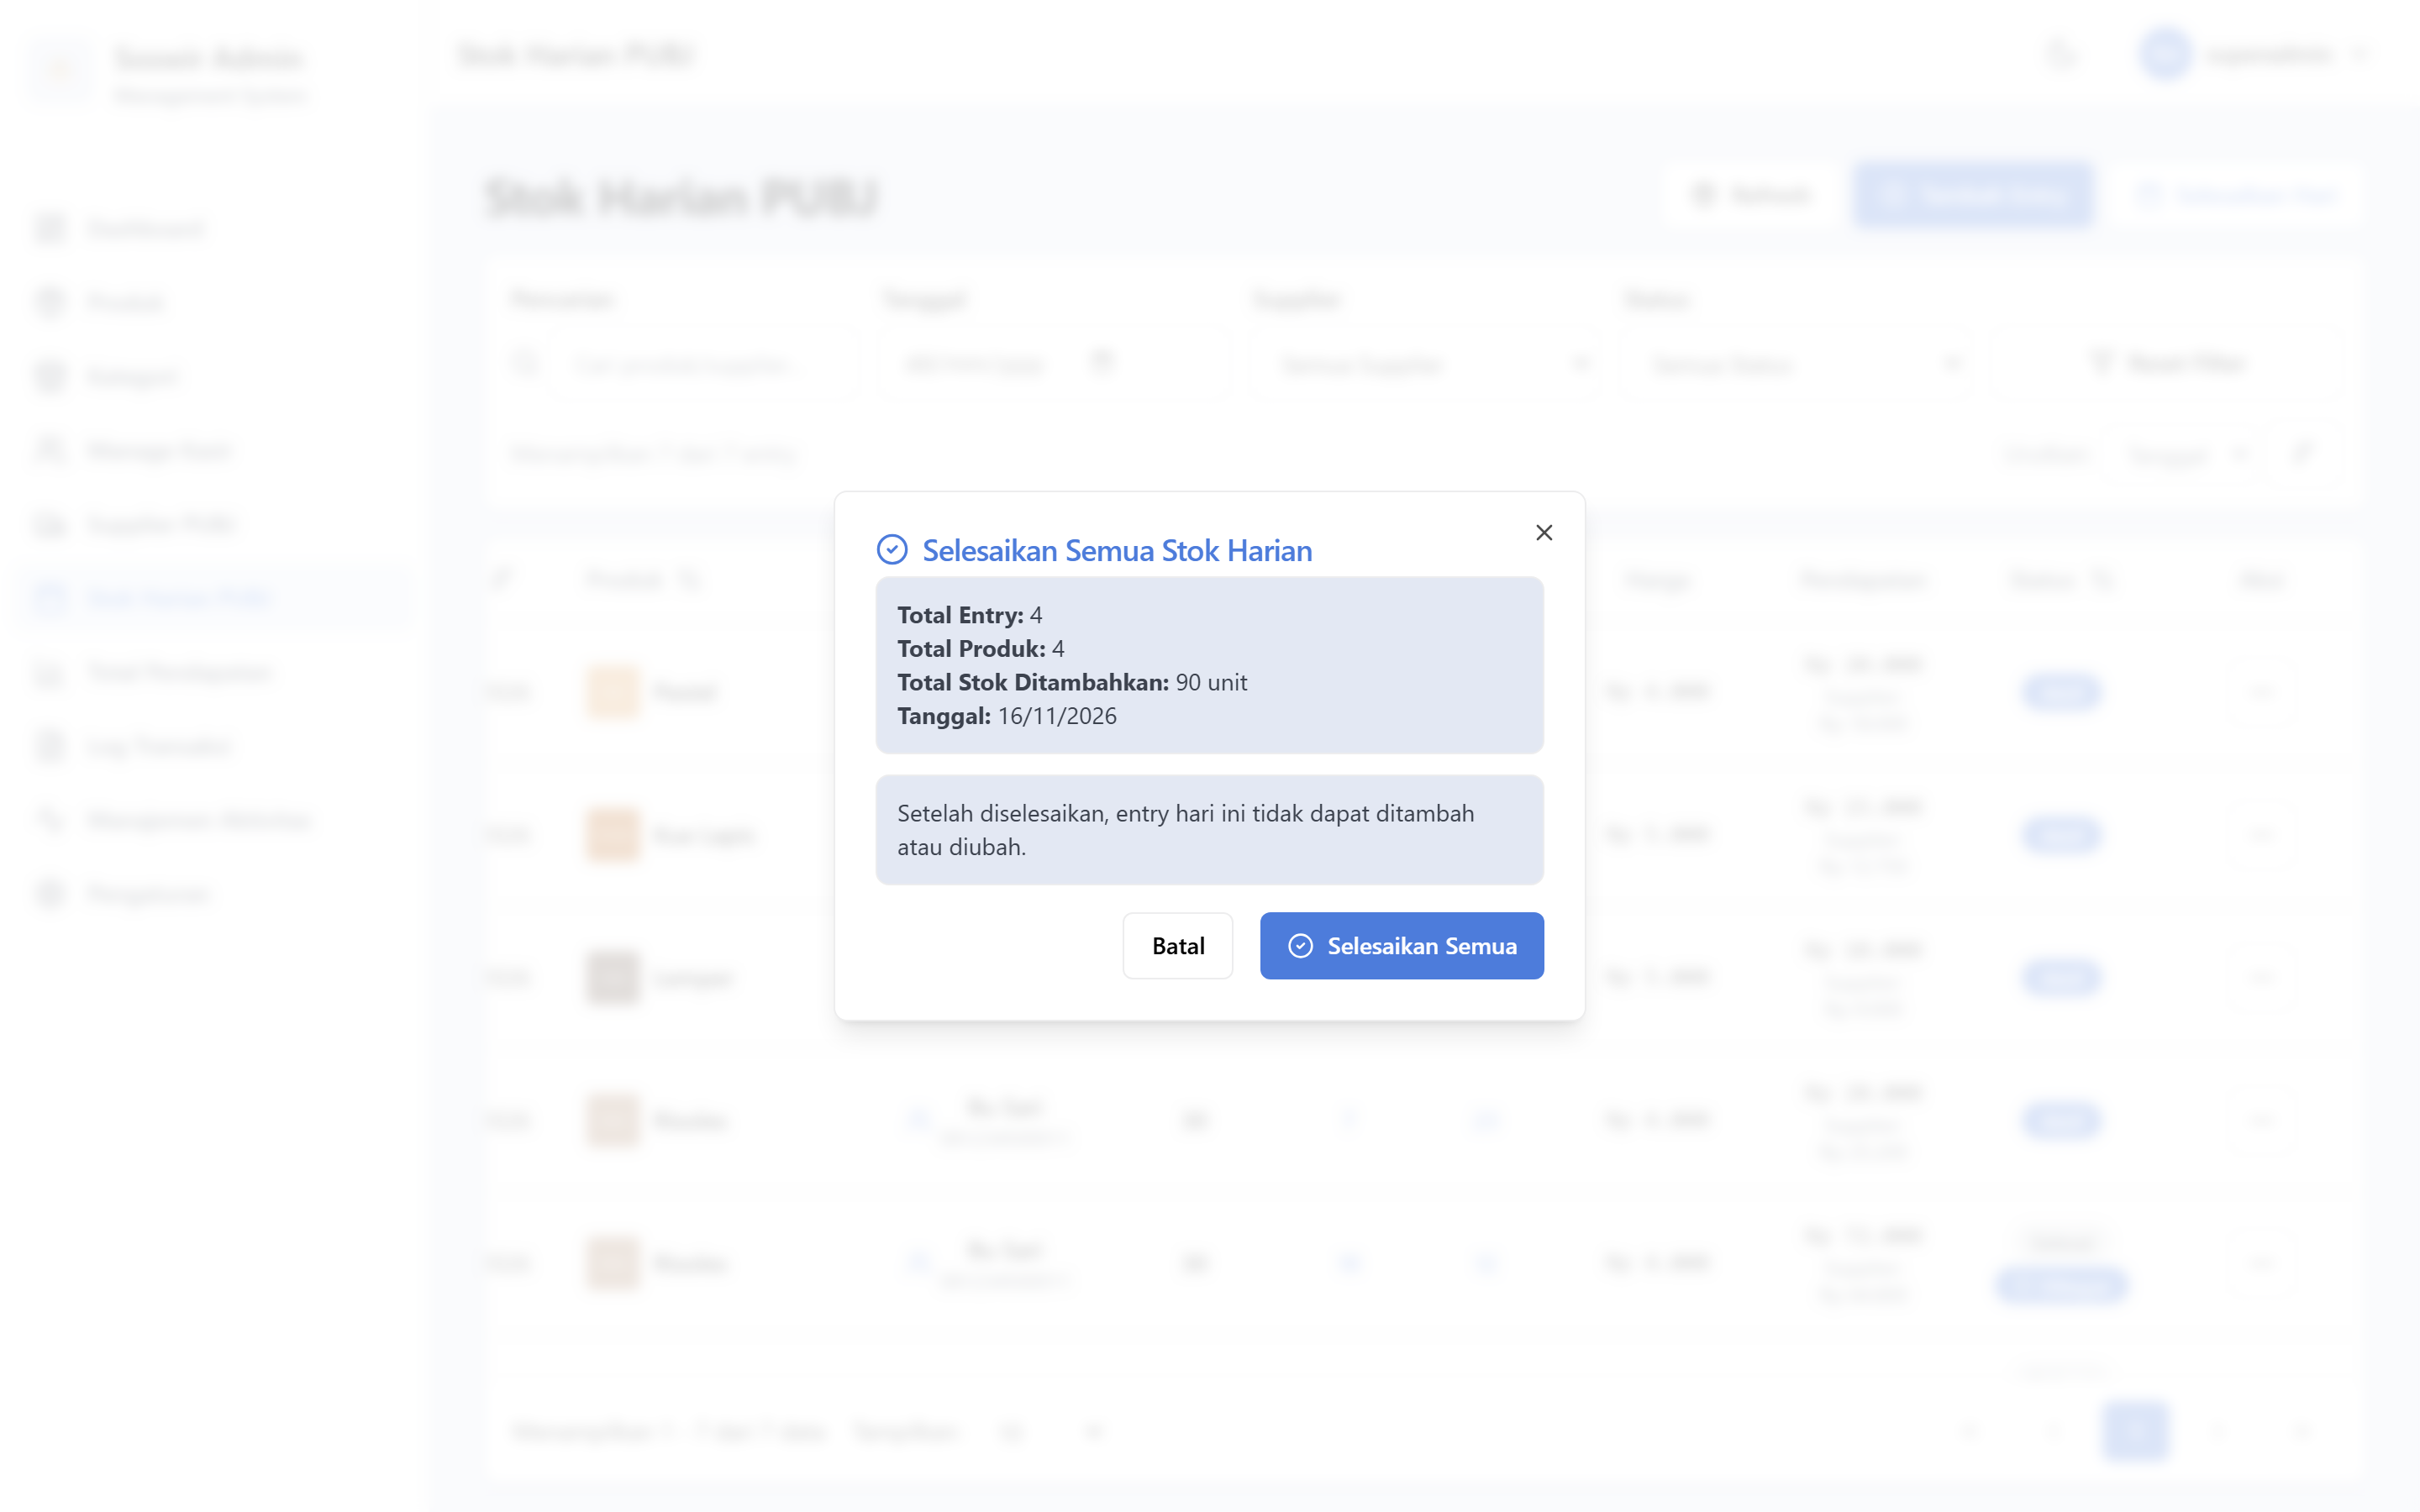
\includegraphics[width=0.99\linewidth,height=0.40\textheight,keepaspectratio,cfbox=garis 0.5pt 0pt]{img/31-stok-harian-selesaikan-hari.png}
\caption{Konfirmasi \ui{Selesaikan Semua Stok Harian}.}
\end{figure}

Setelah diselesaikan, entry hari itu tidak bisa ditambah atau diubah lagi.

\subsection{Menandai pembayaran ke supplier}

Setelah bagian supplier dibayarkan, tandai entry-nya supaya tidak terbayar dua kali.

\begin{enumerate}
  \item Cari entry berstatus \ui{Selesai} dan \ui{Belum Bayar}. Isi kotak \ui{Tanggal} untuk menampilkan entry hari tertentu.
  \item Buka menu aksi entry, pilih \ui{Tandai Dibayar}.
  \item Periksa \ui{Pendapatan Supplier}, lalu tekan \ui{Tandai Dibayar}.
\end{enumerate}

\begin{figure}[H]
\centering
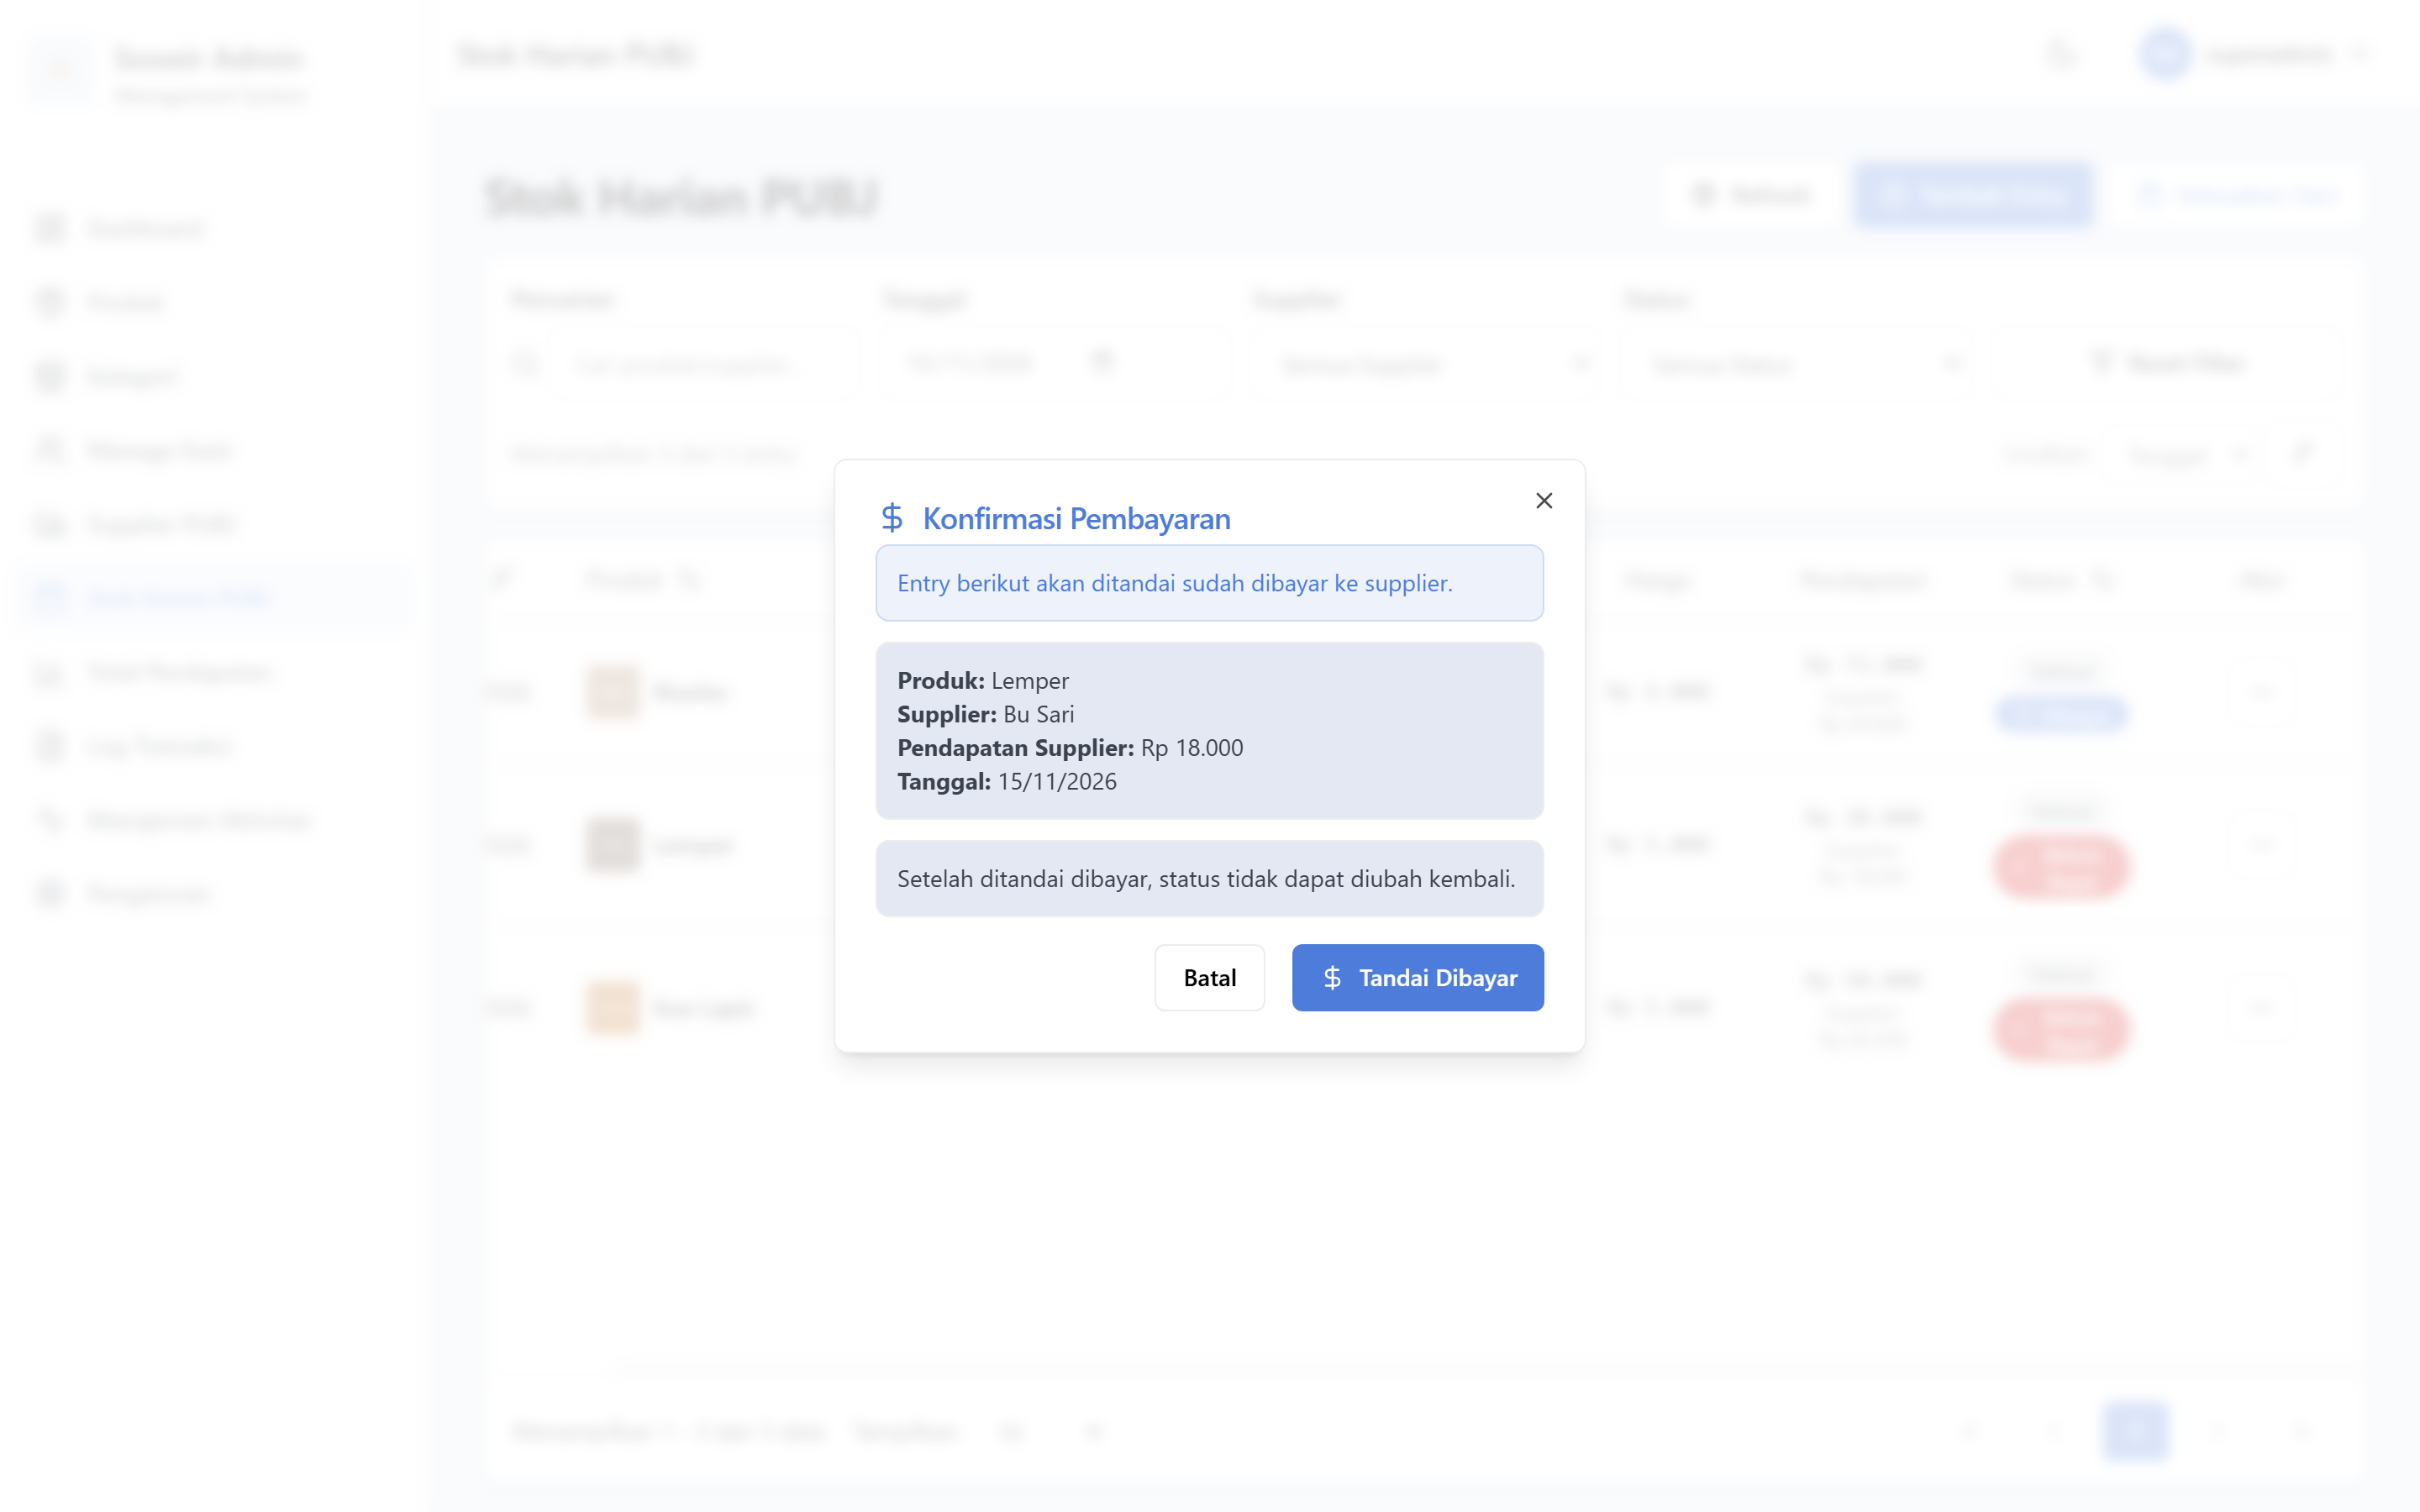
\includegraphics[width=0.99\linewidth,height=0.40\textheight,keepaspectratio,cfbox=garis 0.5pt 0pt]{img/32-stok-harian-tandai-dibayar.png}
\caption{Jendela \ui{Konfirmasi Pembayaran}.}
\end{figure}

Status \ui{Dibayar} tidak bisa dikembalikan, jadi pastikan uangnya memang sudah diserahkan.

% ---------------------------------------------------------------
\section{Manage Kasir}

Menu \ui{Manage Kasir} membuka halaman \ui{Manajemen Kasir}. Kasir dikelompokkan per sesi shift. Setiap kelompok menampilkan nama sesi, jam berlakunya, dan jumlah kasir.

\begin{figure}[H]
\centering
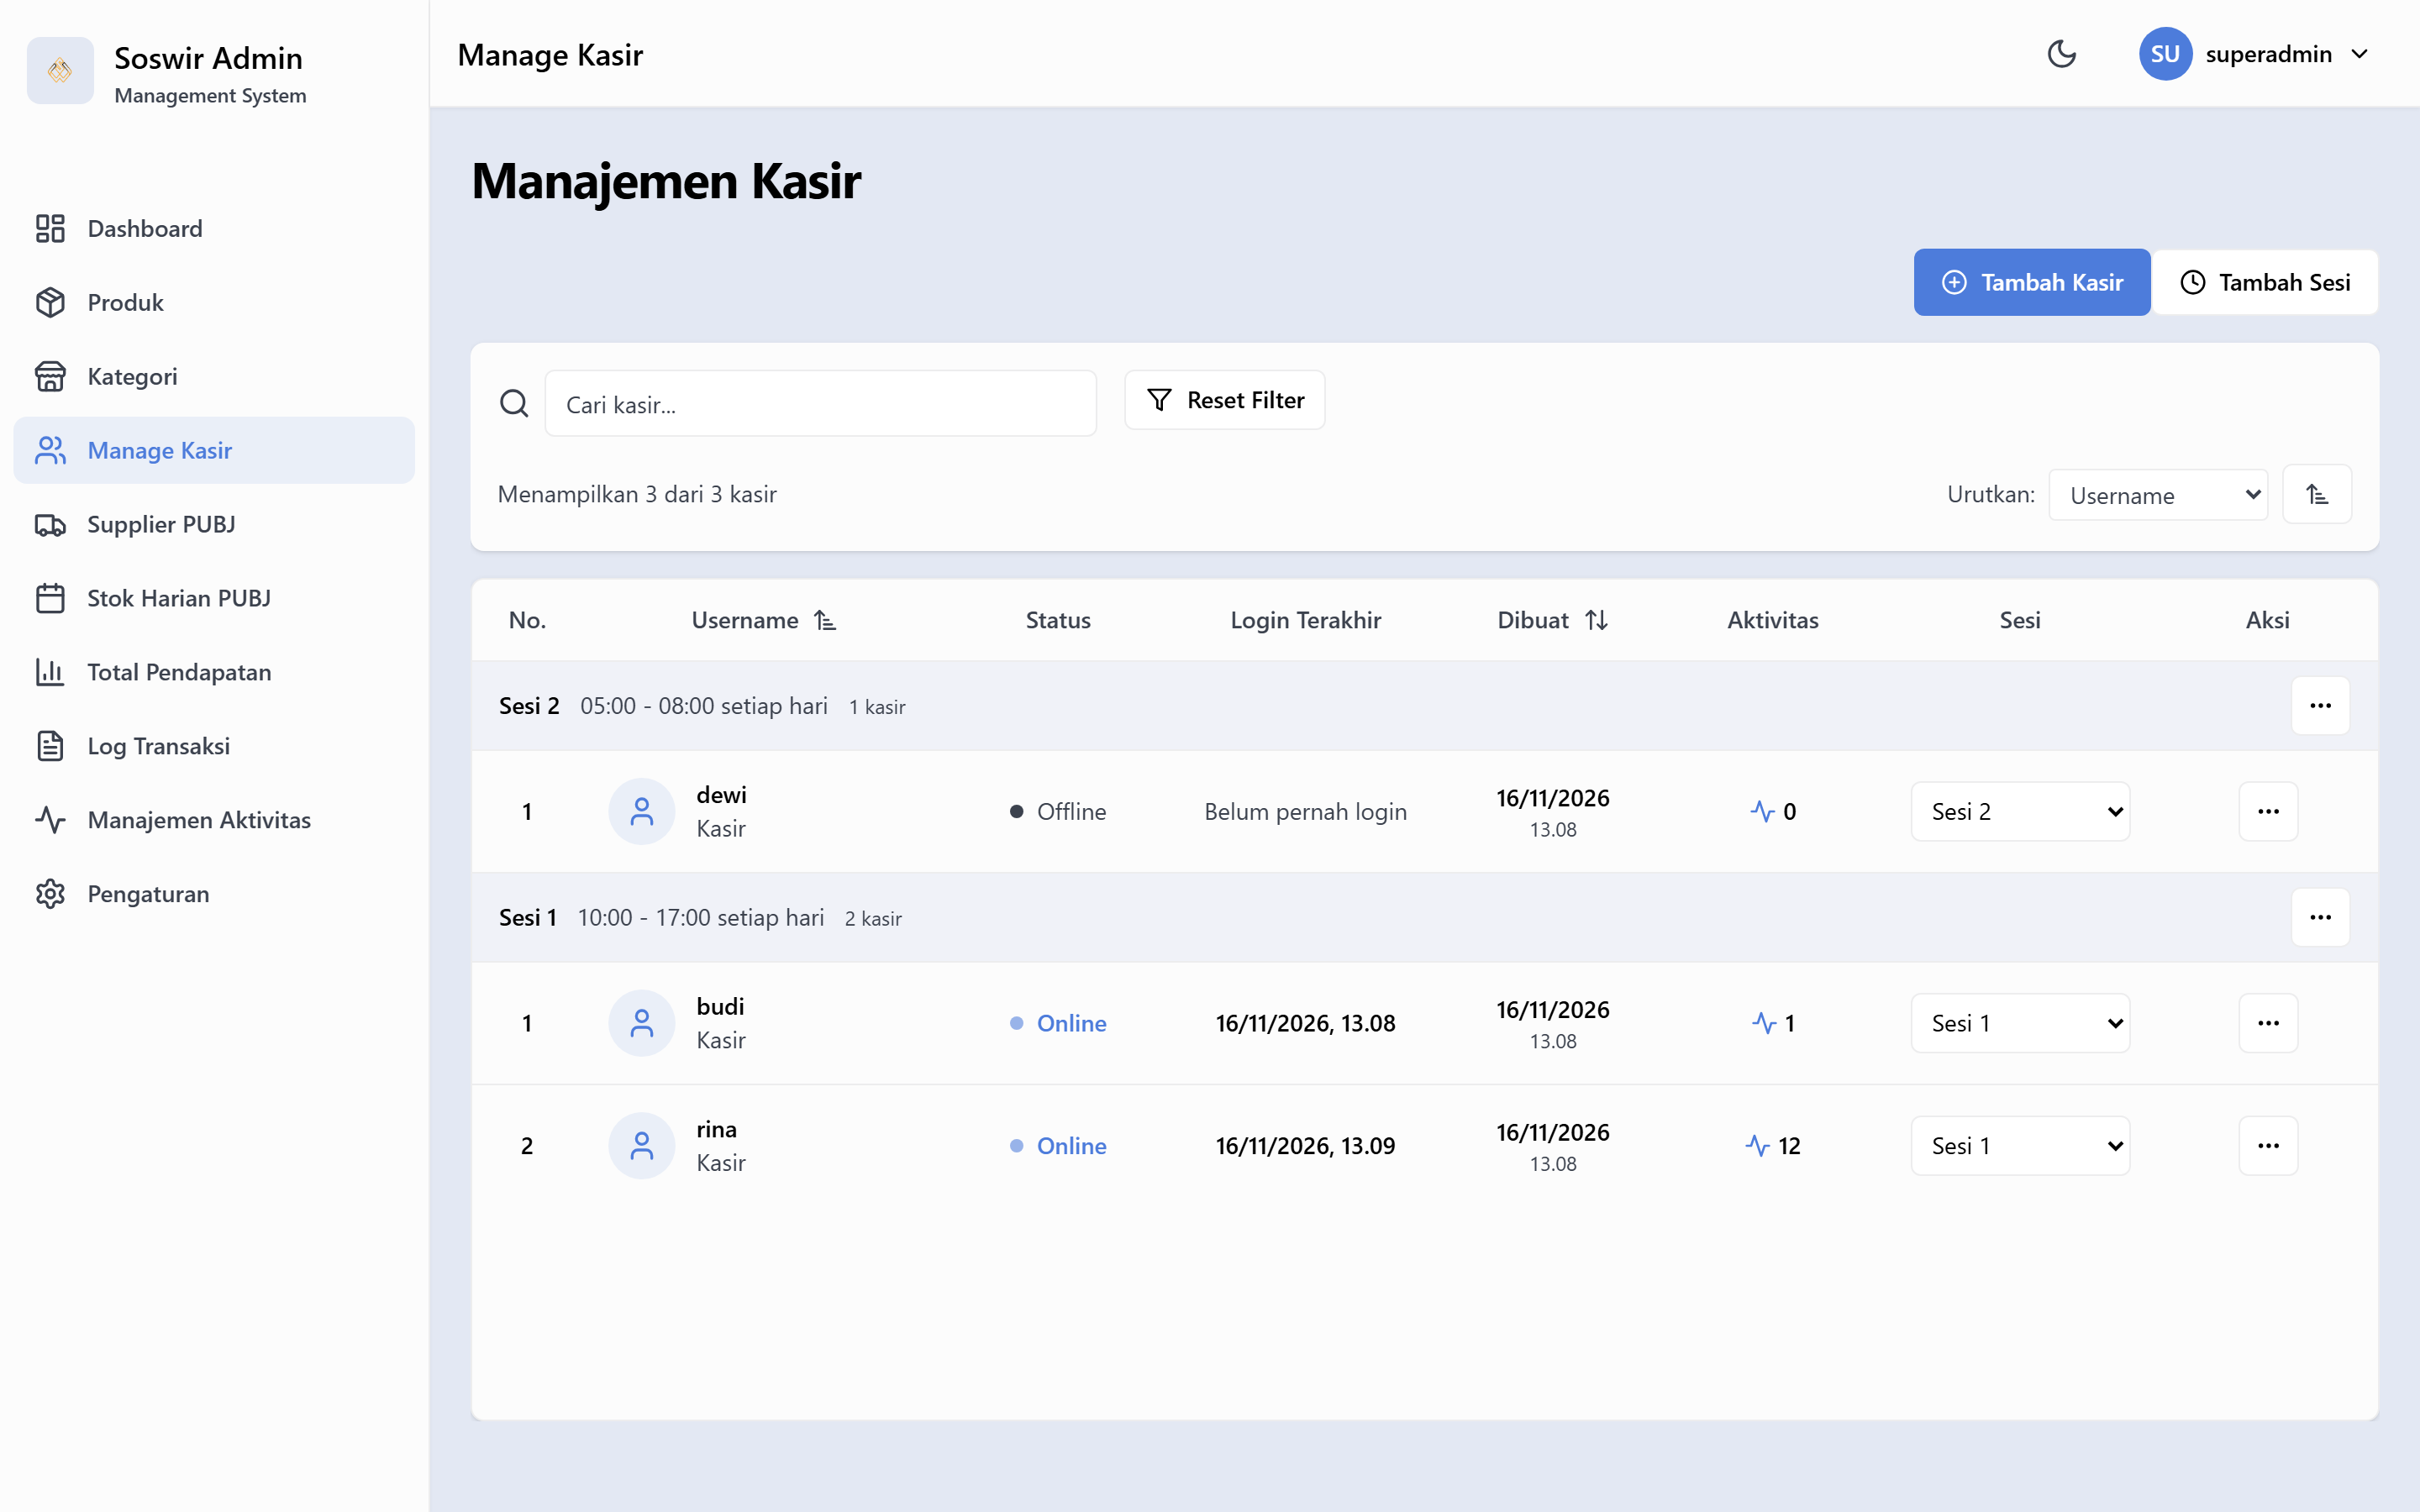
\includegraphics[width=0.99\linewidth,height=0.40\textheight,keepaspectratio,cfbox=garis 0.5pt 0pt]{img/33-kasir-daftar.png}
\caption{Daftar kasir per sesi. Kolom \ui{Status} menunjukkan kasir yang sedang \ui{Online}.}
\end{figure}

\subsection{Membuat sesi shift}

\begin{enumerate}
  \item Tekan \ui{Tambah Sesi}.
  \item Isi \ui{Nama sesi}, \ui{Jam mulai}, dan \ui{Jam selesai}. Jam berlaku setiap hari.
  \item Tekan \ui{Simpan}.
\end{enumerate}

\begin{figure}[H]
\centering
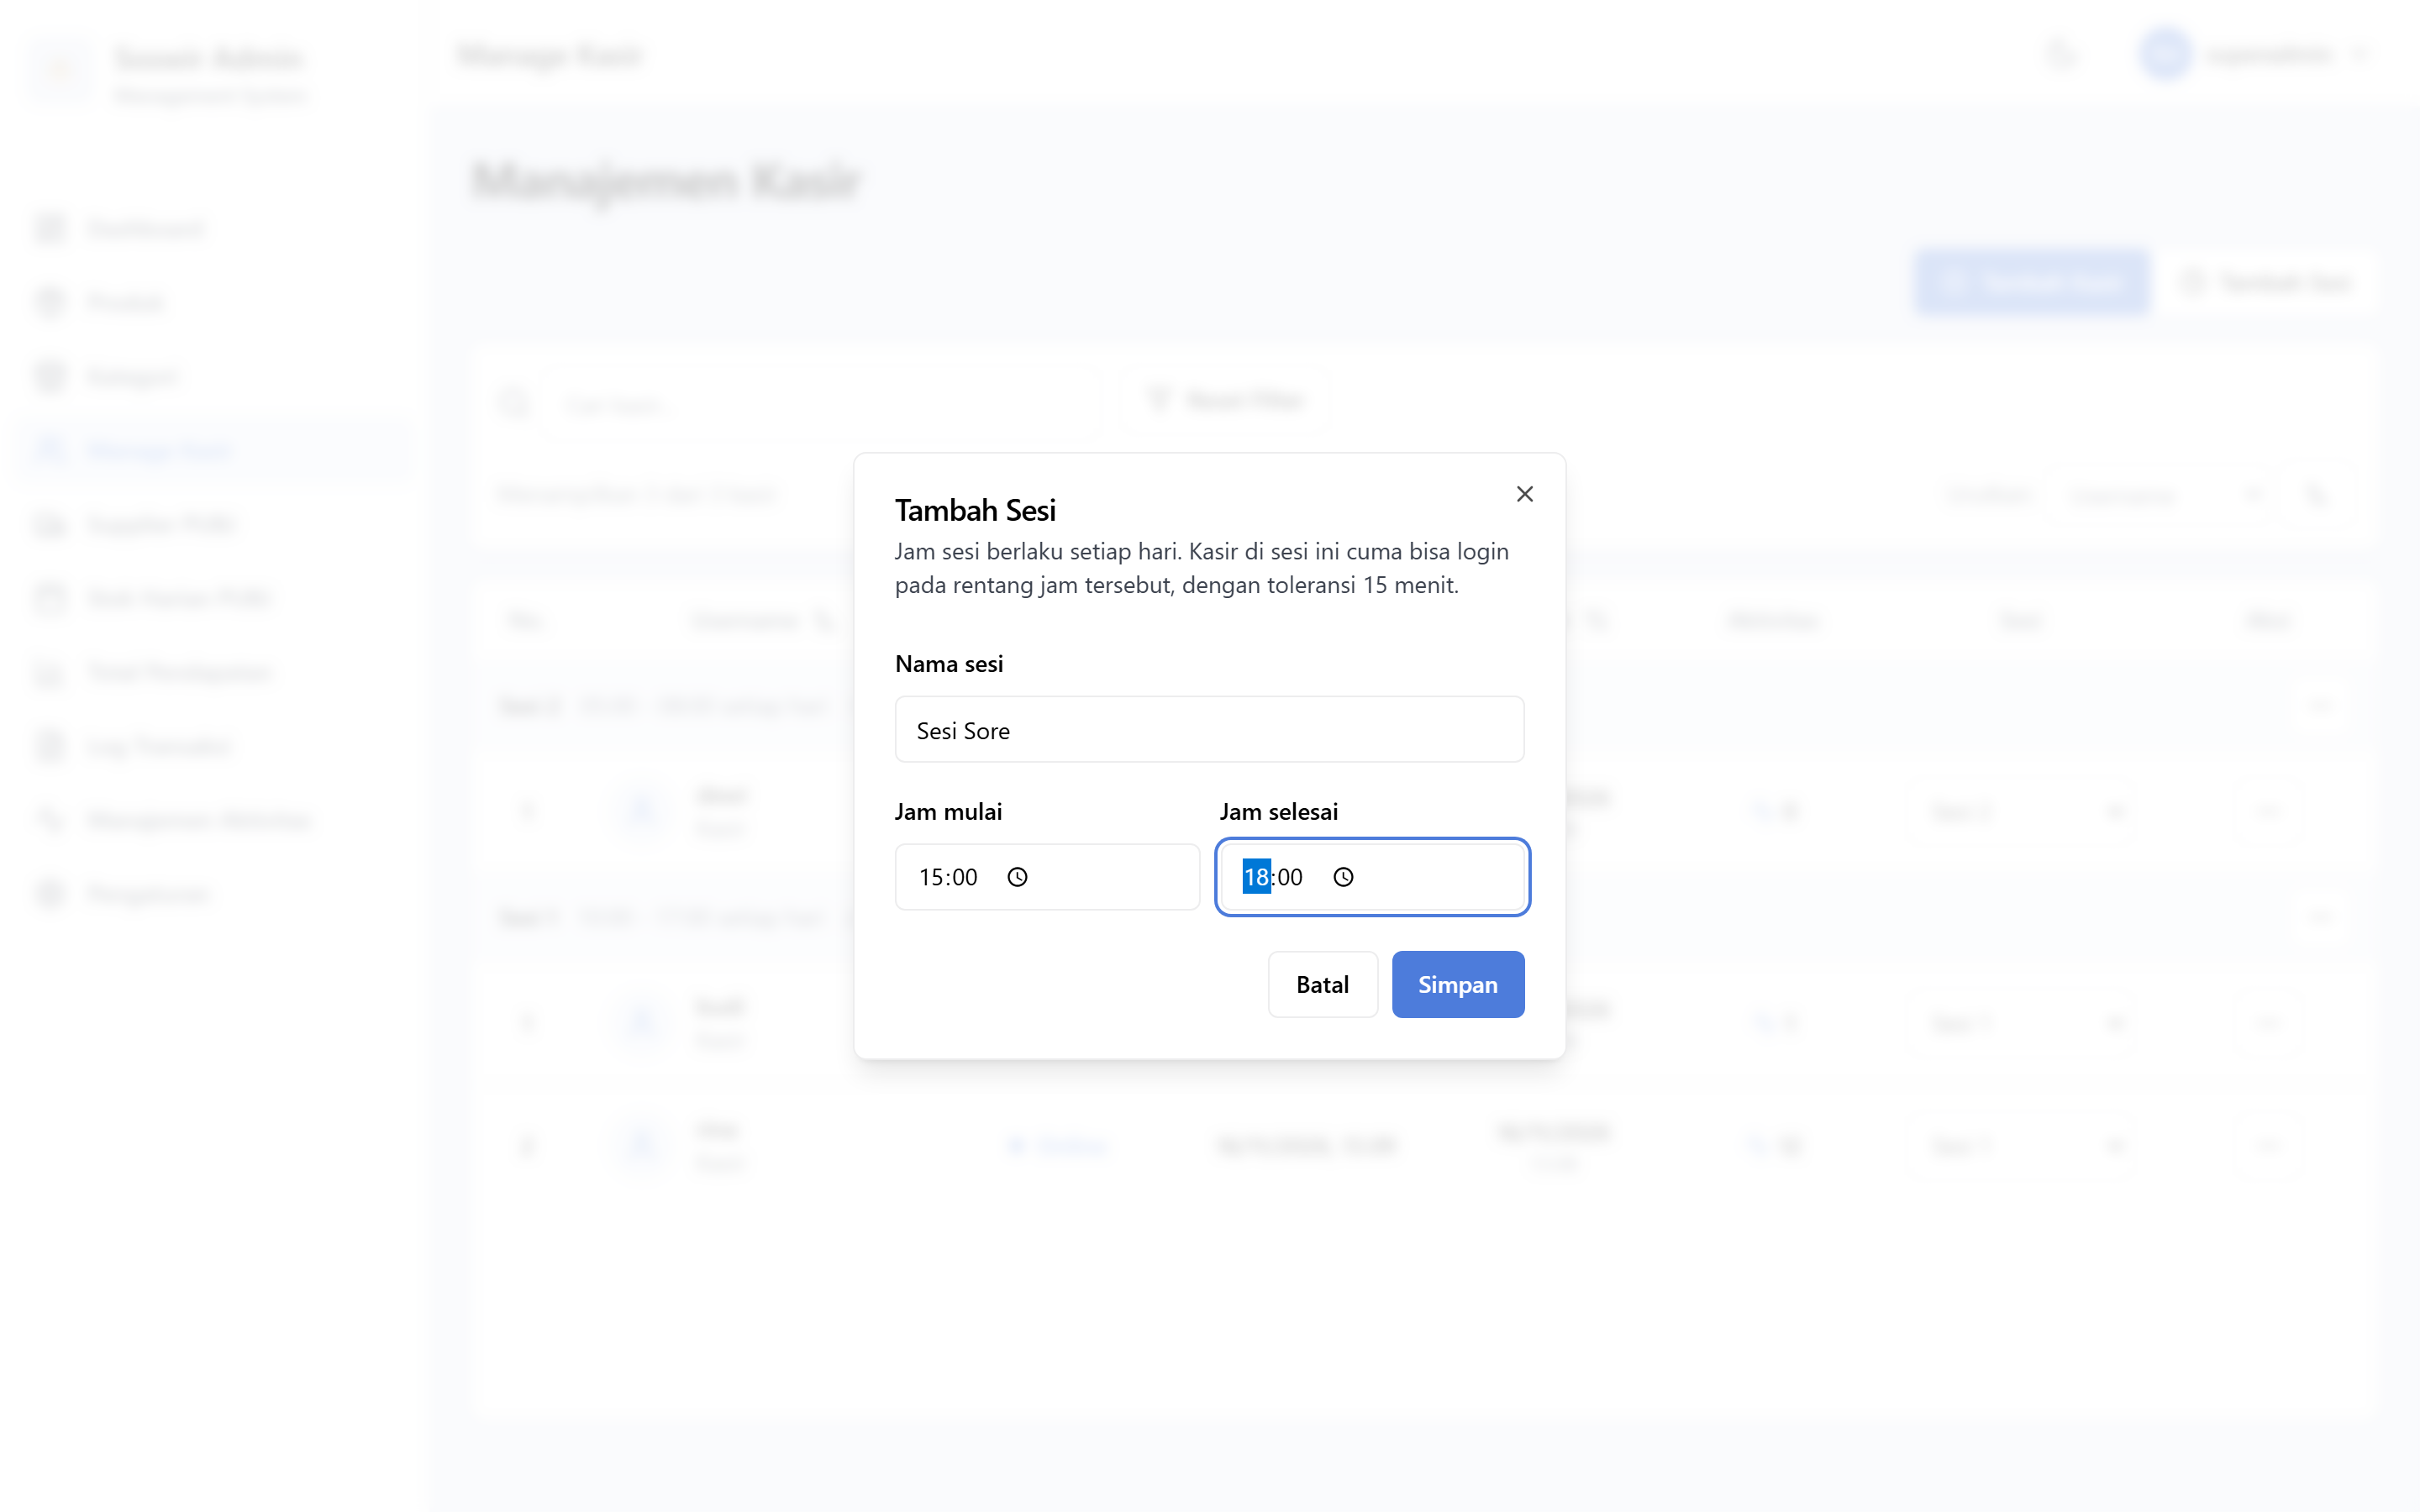
\includegraphics[width=0.99\linewidth,height=0.40\textheight,keepaspectratio,cfbox=garis 0.5pt 0pt]{img/35-sesi-tambah.png}
\caption{Jendela \ui{Tambah Sesi}.}
\end{figure}

Untuk mengubah atau menghapus sesi, tekan tombol tiga titik di baris judul sesi, lalu pilih \ui{Edit sesi} atau \ui{Hapus sesi}. Kasir di sesi yang dihapus menjadi tanpa jadwal dan tidak bisa masuk sampai dipindahkan ke sesi lain.

\subsection{Menambah kasir}

\begin{enumerate}
  \item Tekan \ui{Tambah Kasir}.
  \item Isi \ui{Username}, \ui{Password}, dan \ui{Konfirmasi}.
  \item Tekan \ui{Simpan}.
  \item Tempatkan kasir baru di sesinya, seperti di subbab berikut. Kasir baru masuk kelompok \ui{Belum ada sesi} dan belum bisa masuk.
\end{enumerate}

\begin{figure}[H]
\centering
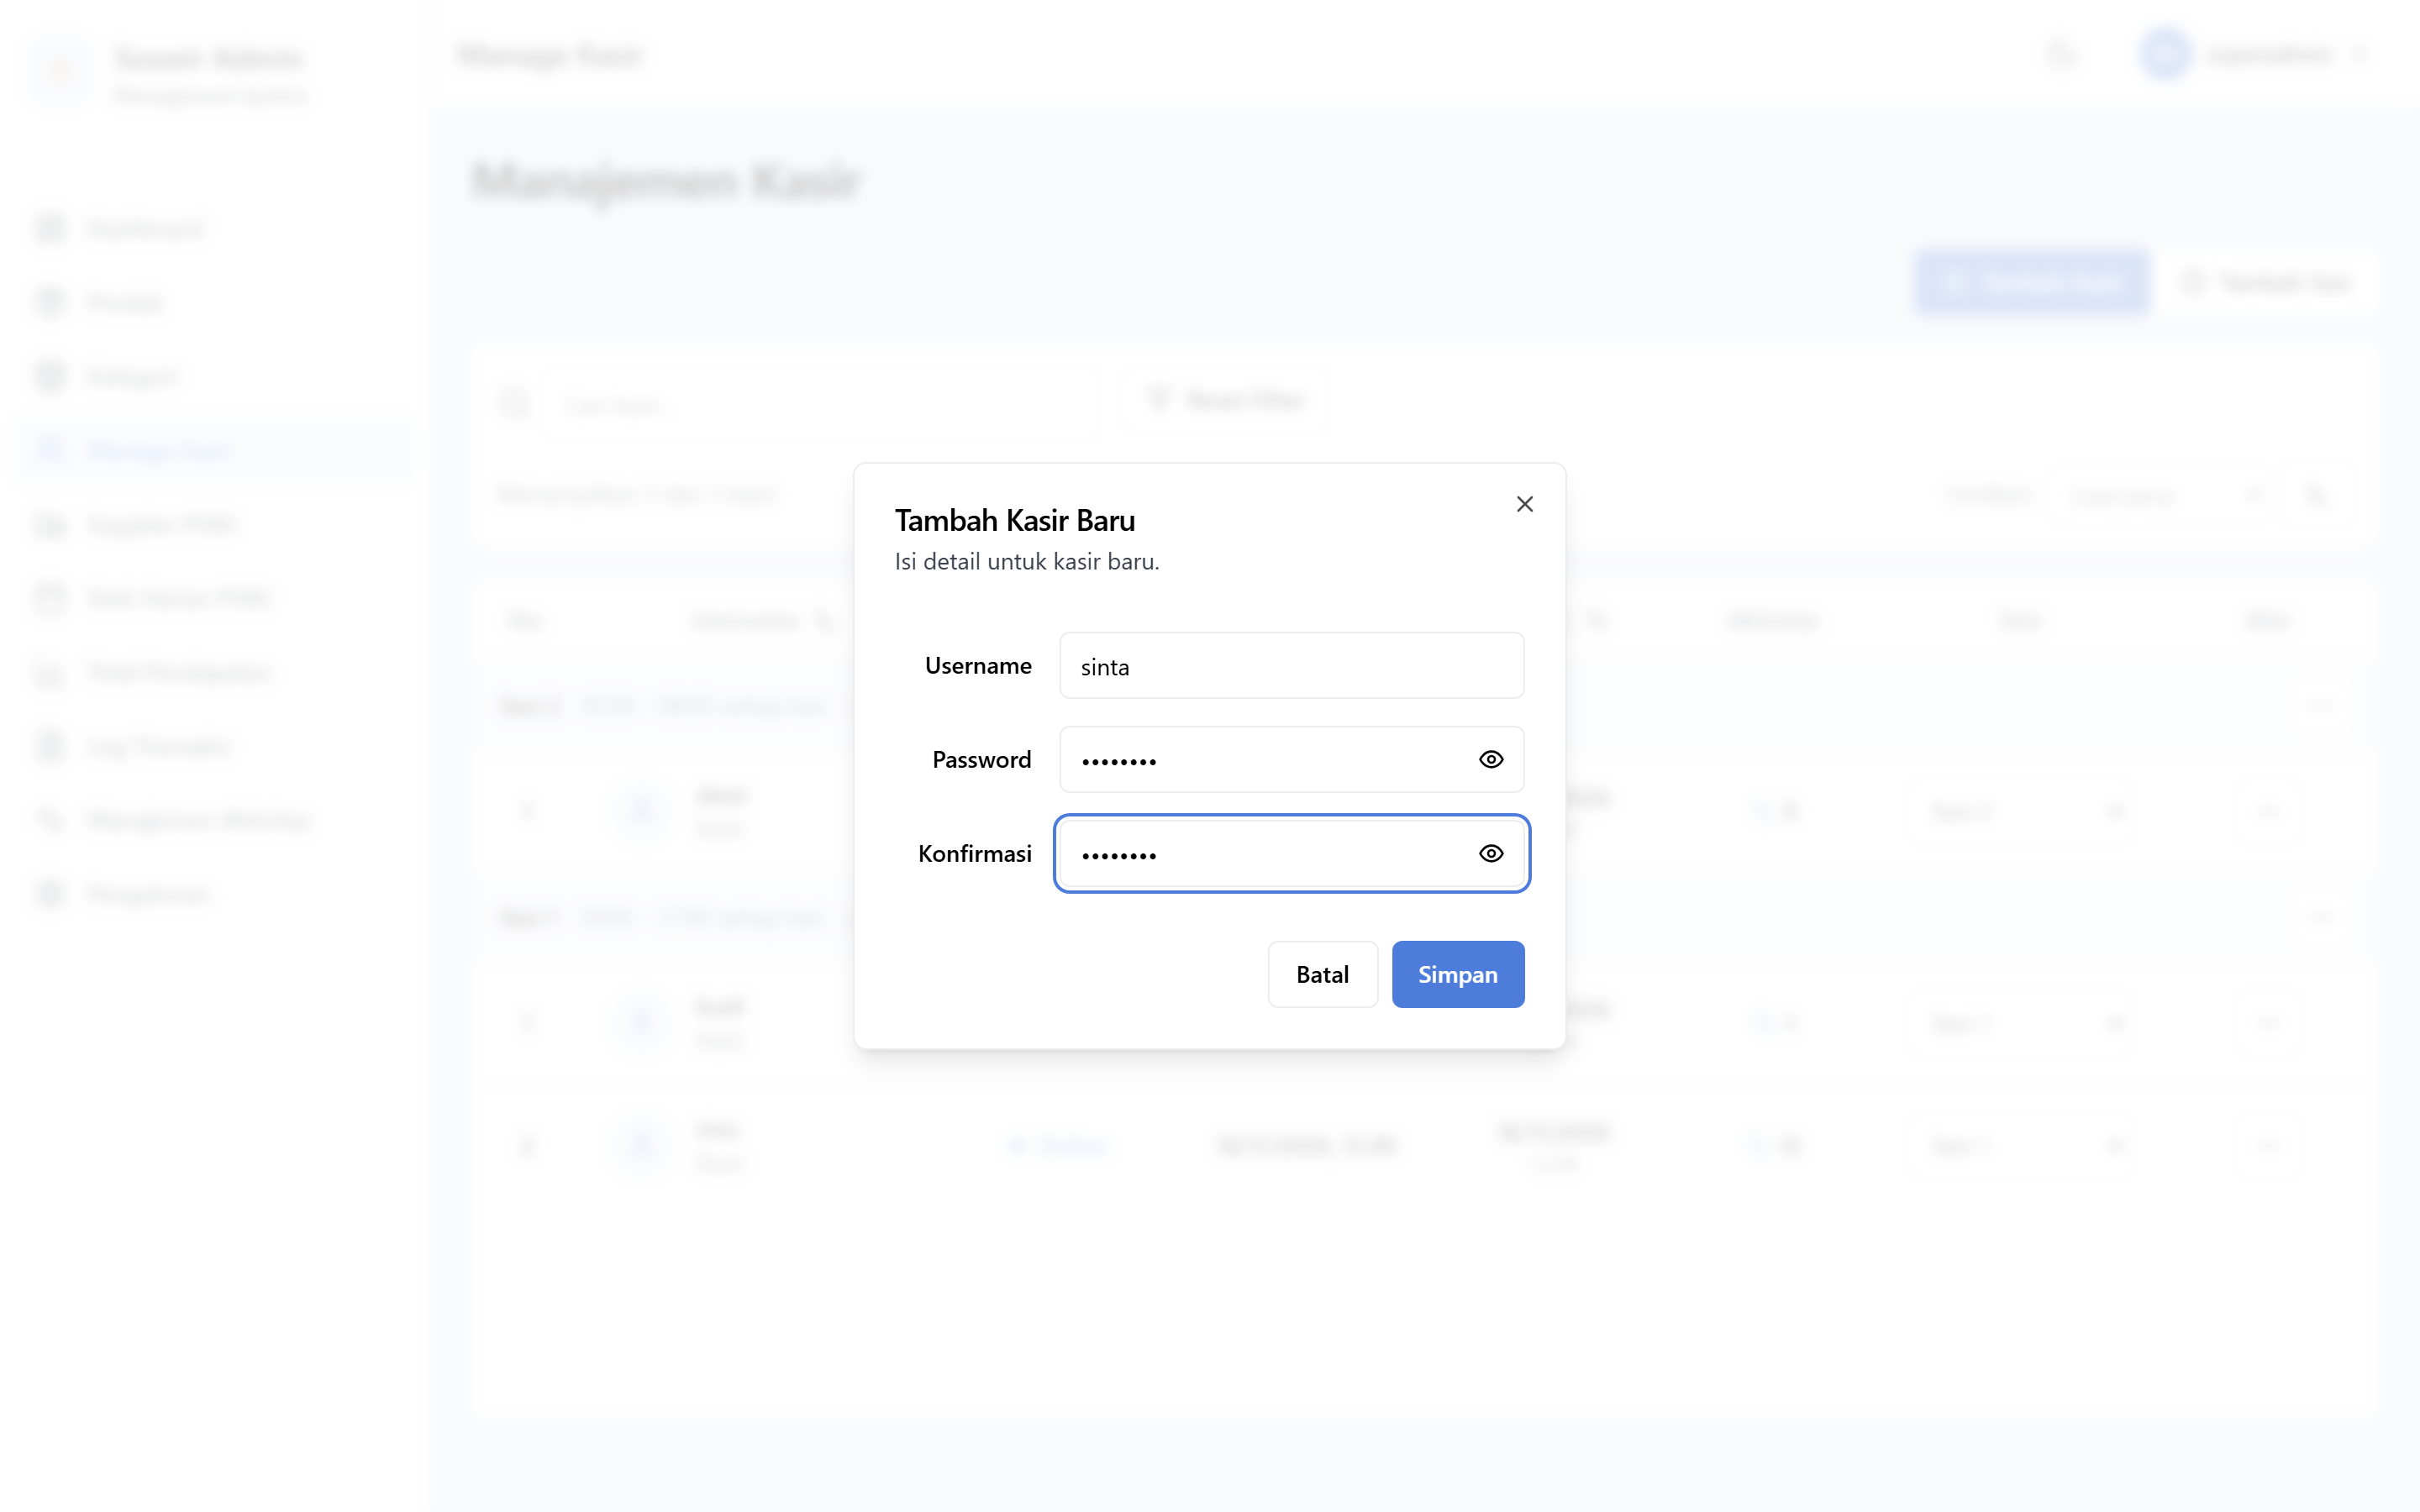
\includegraphics[width=0.99\linewidth,height=0.40\textheight,keepaspectratio,cfbox=garis 0.5pt 0pt]{img/34-kasir-tambah.png}
\caption{Jendela \ui{Tambah Kasir Baru}.}
\end{figure}

\subsection{Menempatkan kasir ke sesi}

Pada kolom \ui{Sesi} di baris kasir, pilih nama sesi dari daftar. Perubahan langsung tersimpan dan kasir pindah ke kelompok sesi tersebut. Pilihan \ui{Tanpa sesi} membuat kasir tidak bisa masuk.

\subsection{Mengubah kasir dan mengganti password kasir}

Kalau kasir lupa password, superadmin bisa membuatkan password baru.

\begin{enumerate}
  \item Buka menu aksi kasir, pilih \ui{Edit}.
  \item Ubah \ui{Username} bila perlu.
  \item Isi \ui{Password} dan \ui{Konfirmasi} dengan password baru. Biarkan kosong kalau tidak ingin mengganti password.
  \item Tekan \ui{Simpan}, lalu beri tahu kasir password barunya.
\end{enumerate}

\begin{figure}[H]
\centering
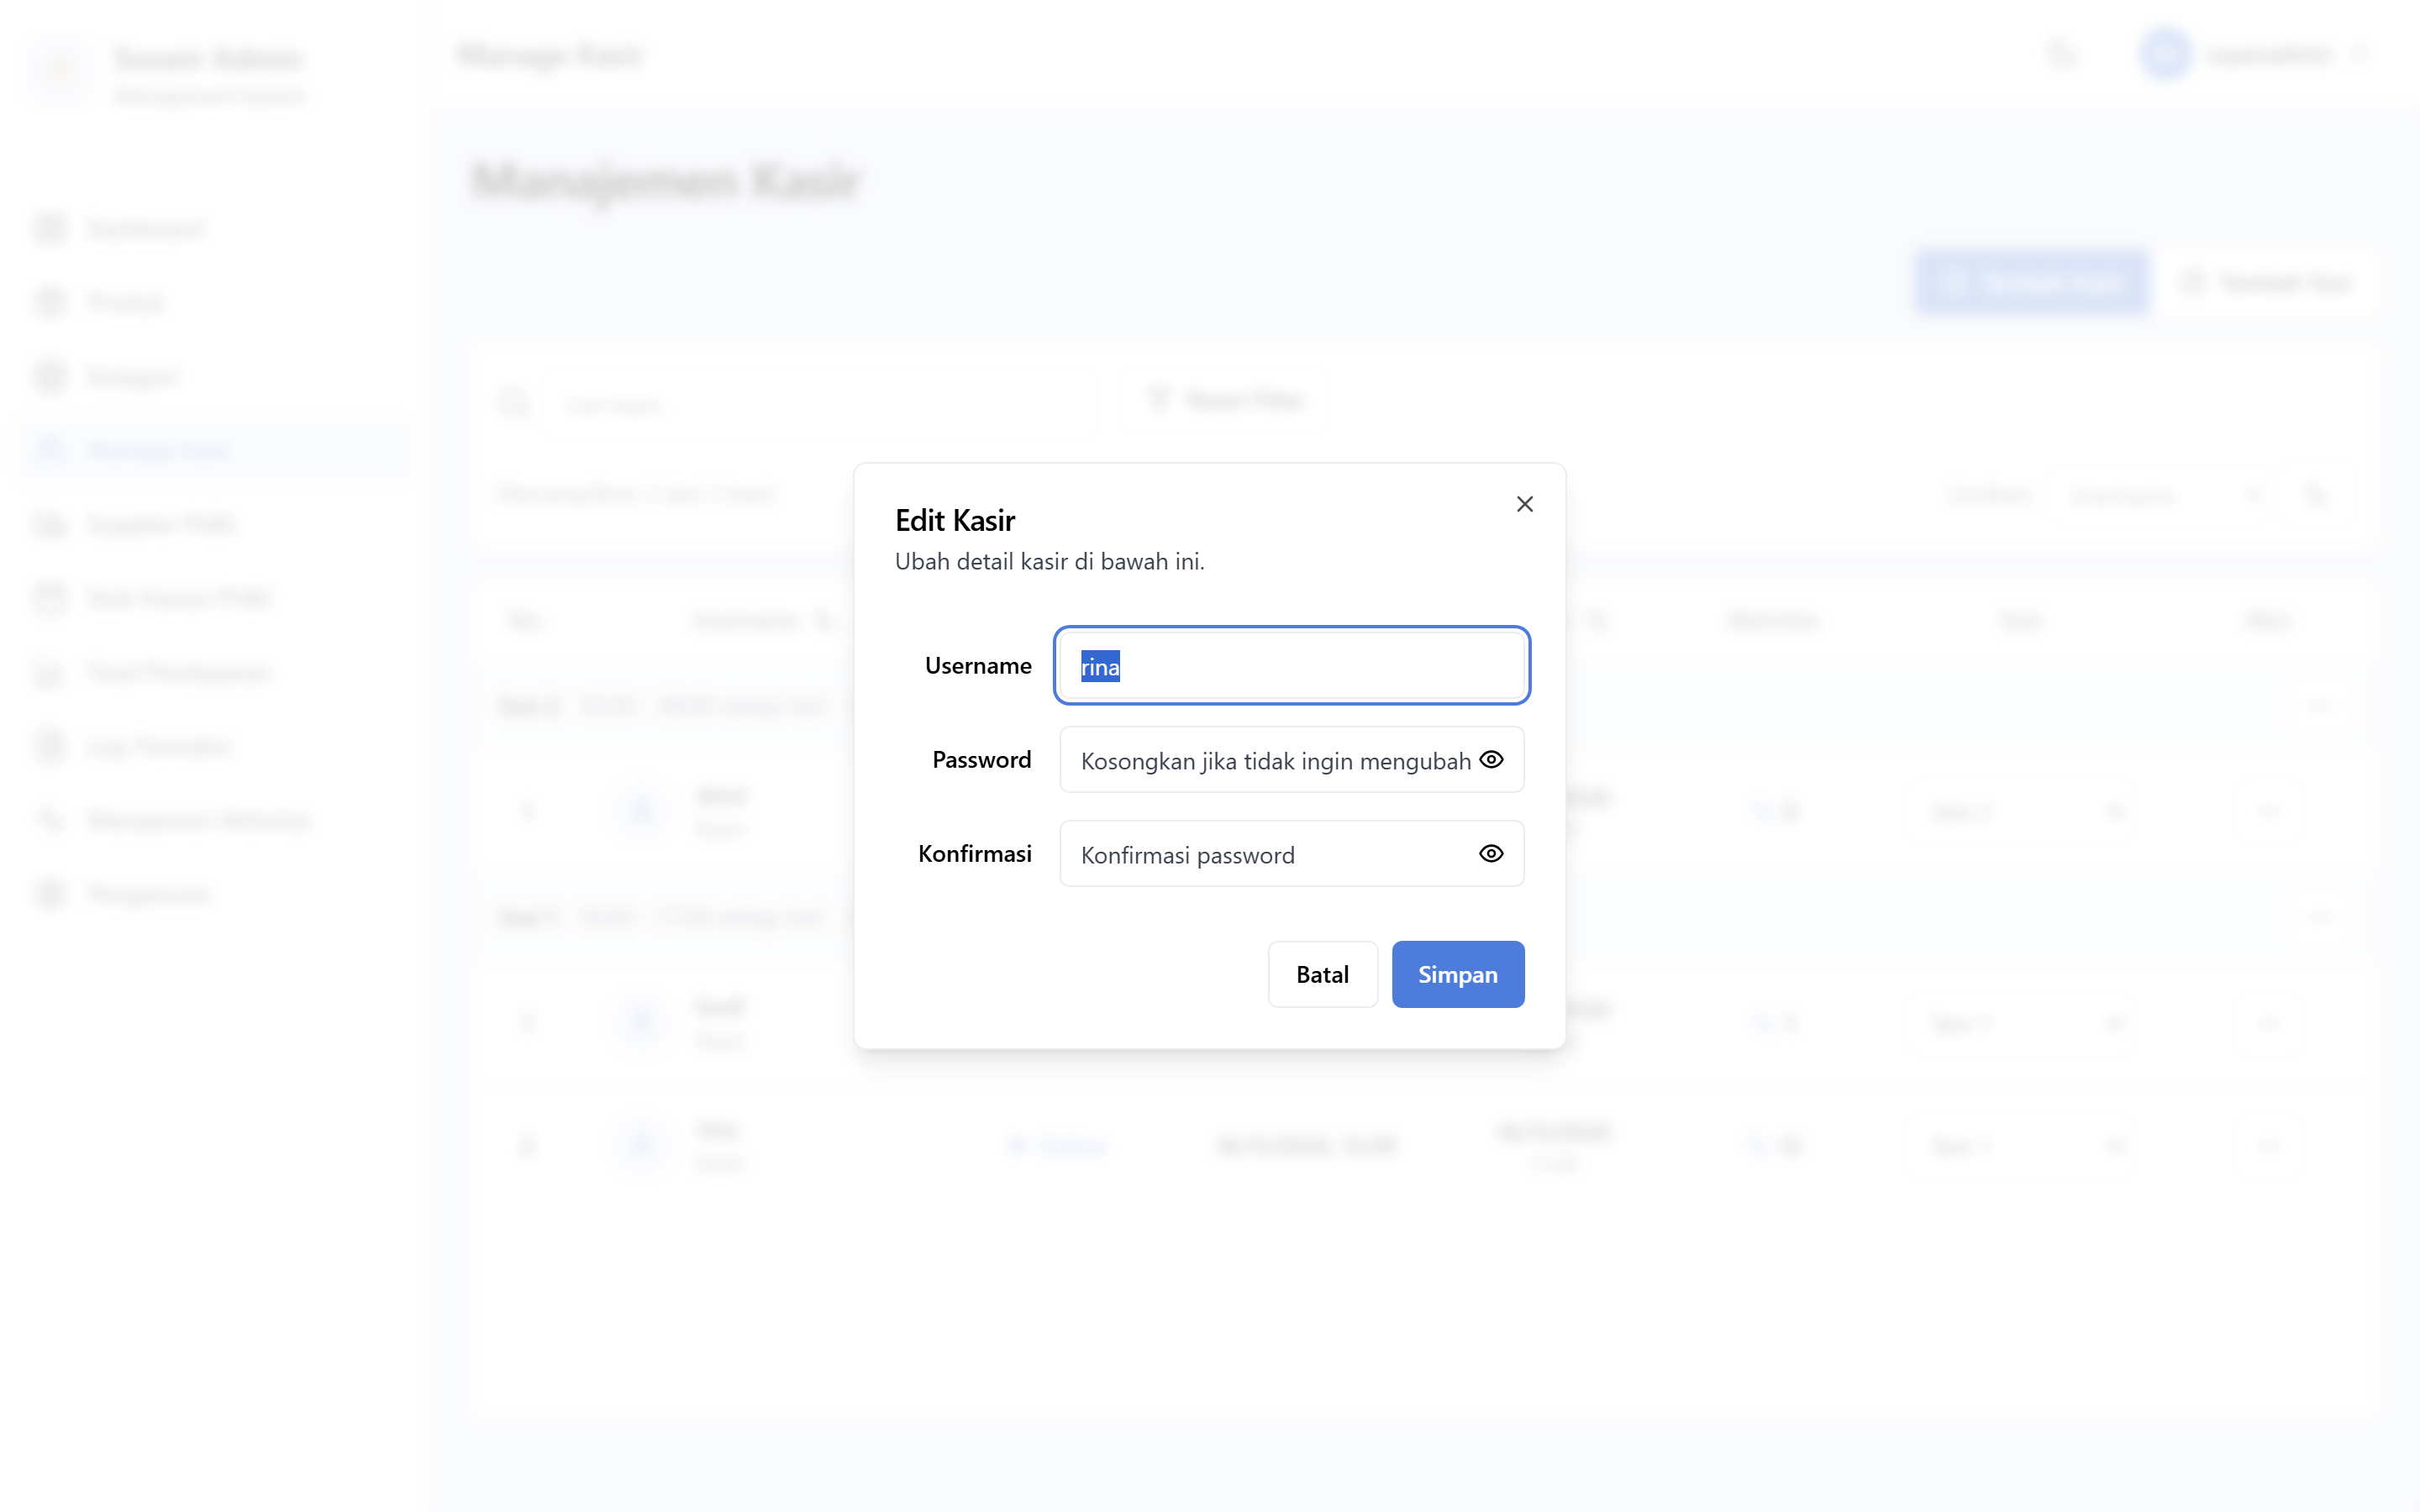
\includegraphics[width=0.99\linewidth,height=0.40\textheight,keepaspectratio,cfbox=garis 0.5pt 0pt]{img/36-kasir-edit.png}
\caption{Jendela \ui{Edit Kasir}.}
\end{figure}

\subsection{Melihat aktivitas kasir}

Pilih \ui{Lihat Aktivitas} pada menu aksi kasir. Jendela \ui{Detail Aktivitas} menampilkan 50 catatan terakhir: kapan kasir \ui{Login}, \ui{Logout}, dan halaman apa saja yang dibuka (\ui{Navigasi}).

\begin{figure}[H]
\centering
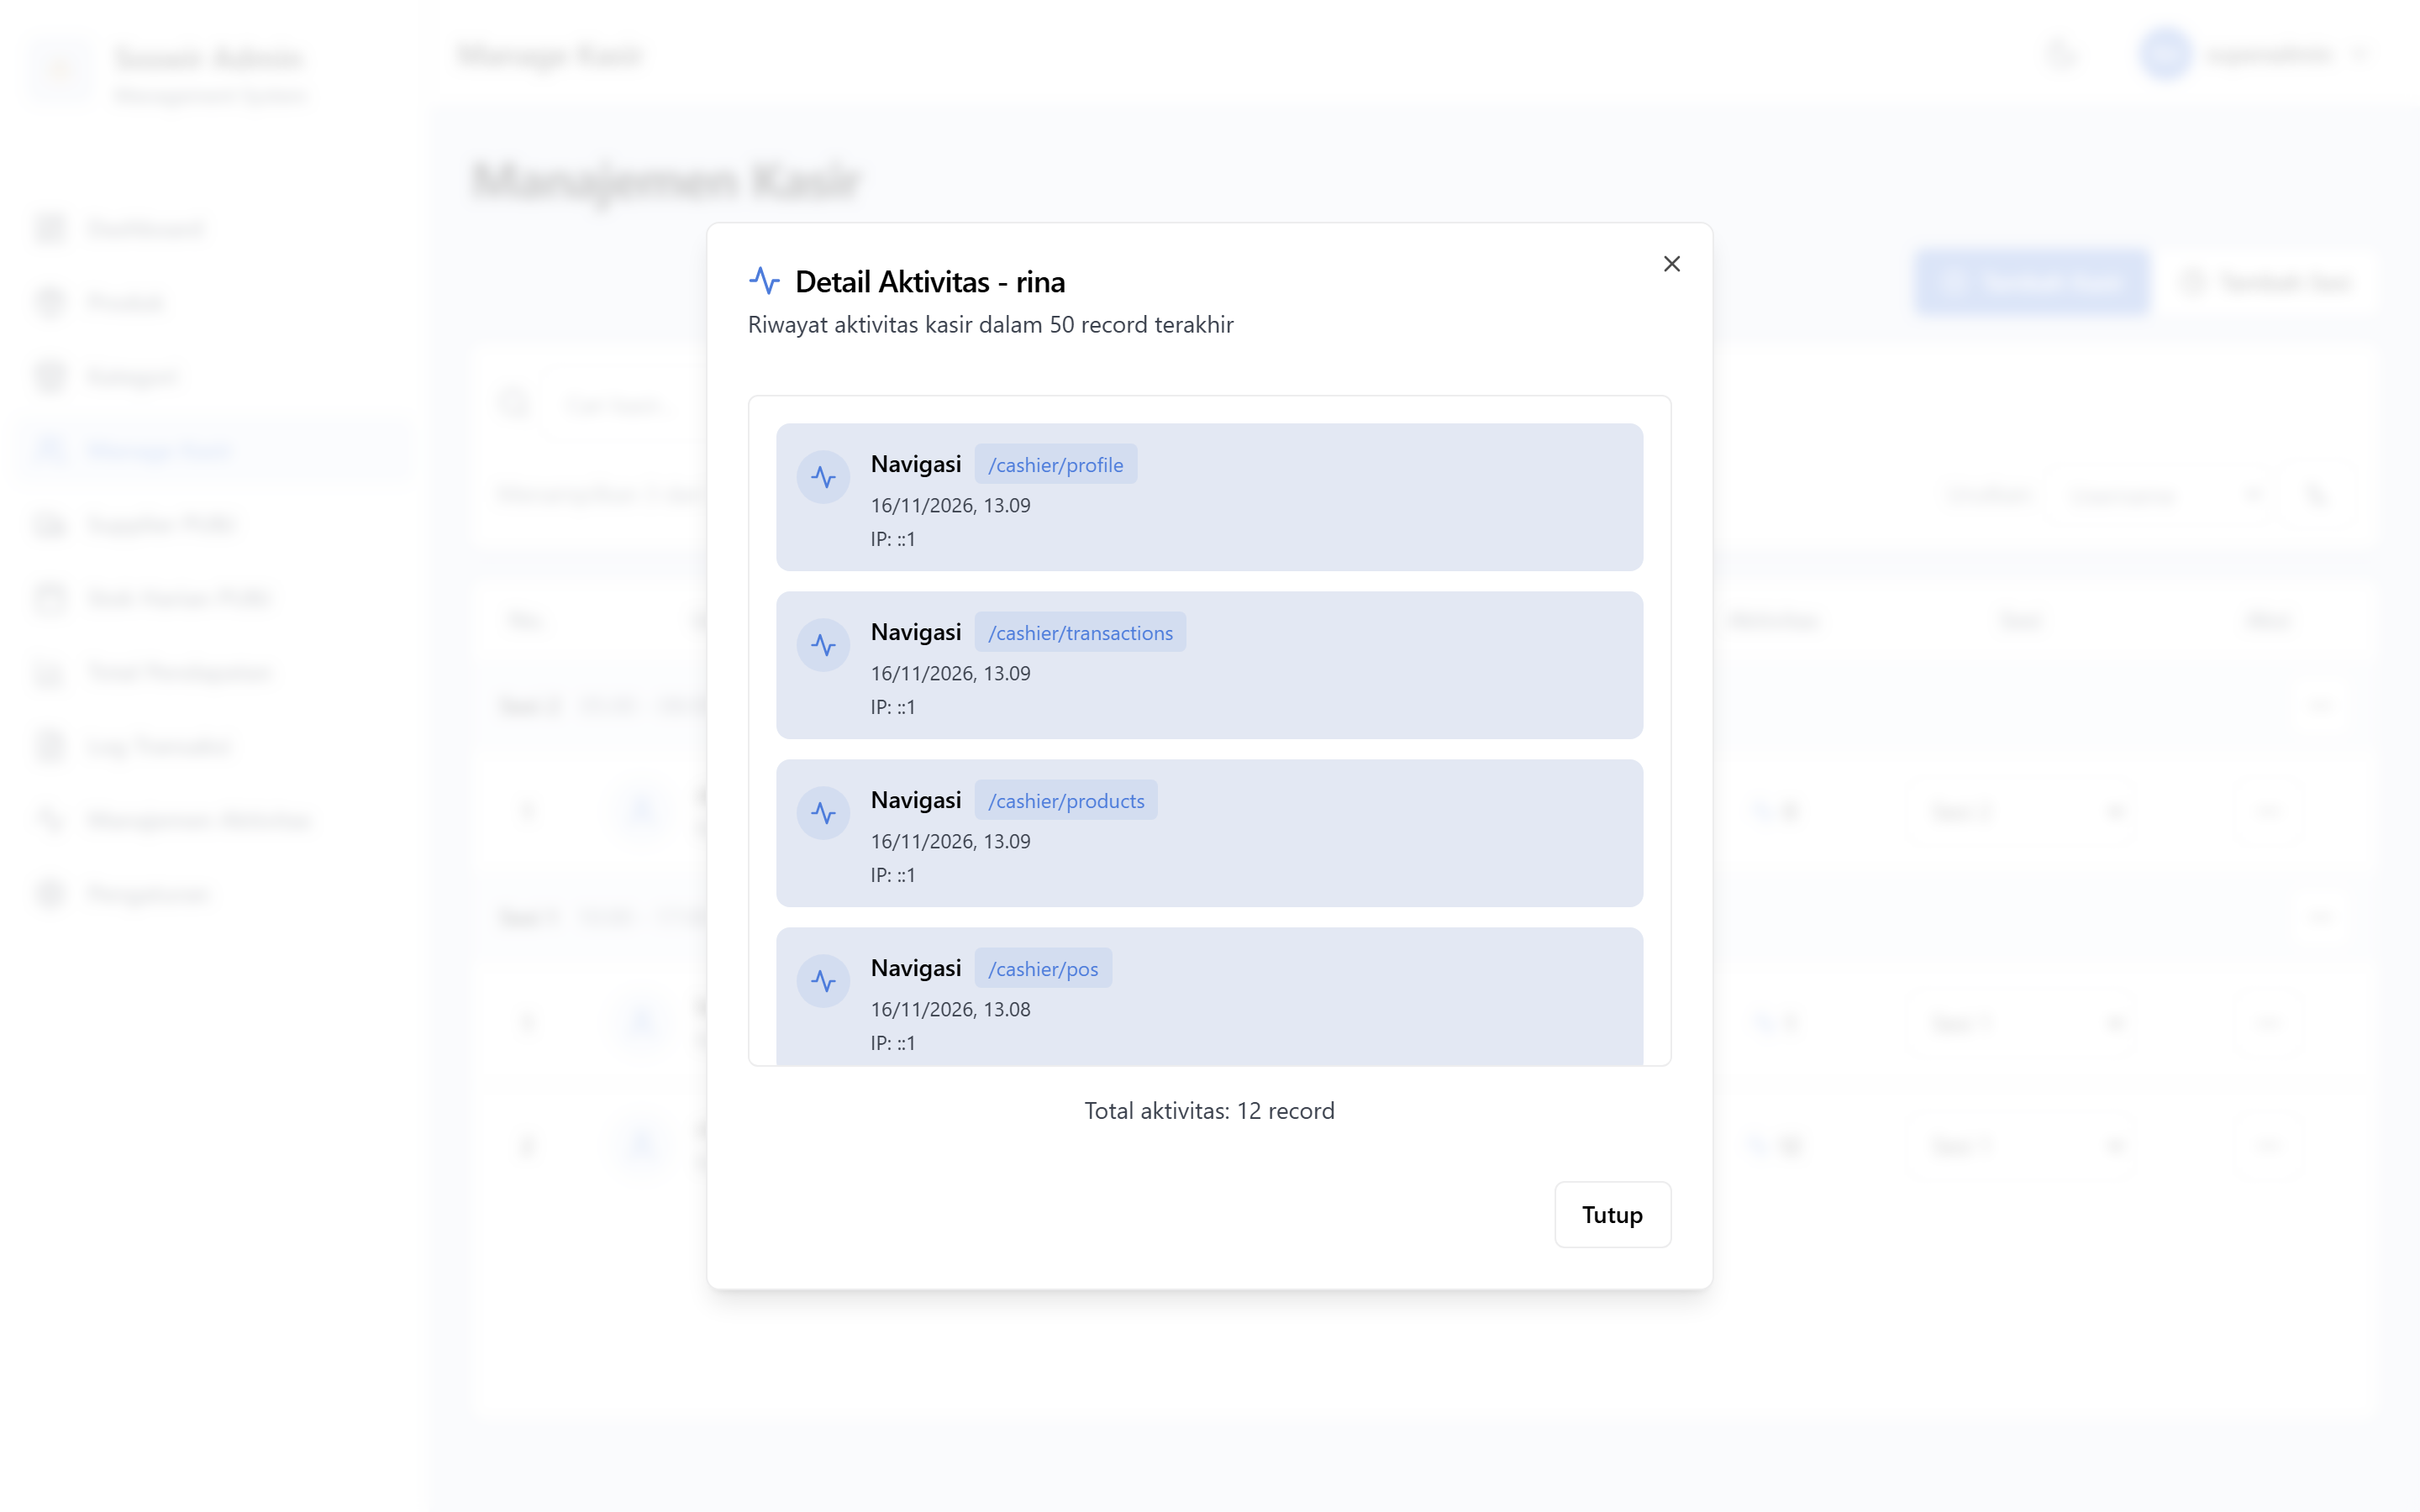
\includegraphics[width=0.99\linewidth,height=0.40\textheight,keepaspectratio,cfbox=garis 0.5pt 0pt]{img/37-kasir-aktivitas.png}
\caption{Riwayat aktivitas kasir.}
\end{figure}

\subsection{Menghapus kasir}

\begin{enumerate}
  \item Buka menu aksi kasir, pilih \ui{Hapus}.
  \item Setujui pertanyaan konfirmasi dari peramban.
\end{enumerate}

Kasir yang sudah pernah mencatat transaksi tidak bisa dihapus, karena riwayat penjualannya harus tetap ada. Aplikasi menampilkan pesan ``Kasir masih punya riwayat transaksi, tidak bisa dihapus''. Untuk kasir yang berhenti bekerja, ganti password-nya dan pindahkan ke \ui{Tanpa sesi} supaya tidak bisa masuk lagi.

\begin{figure}[H]
\centering
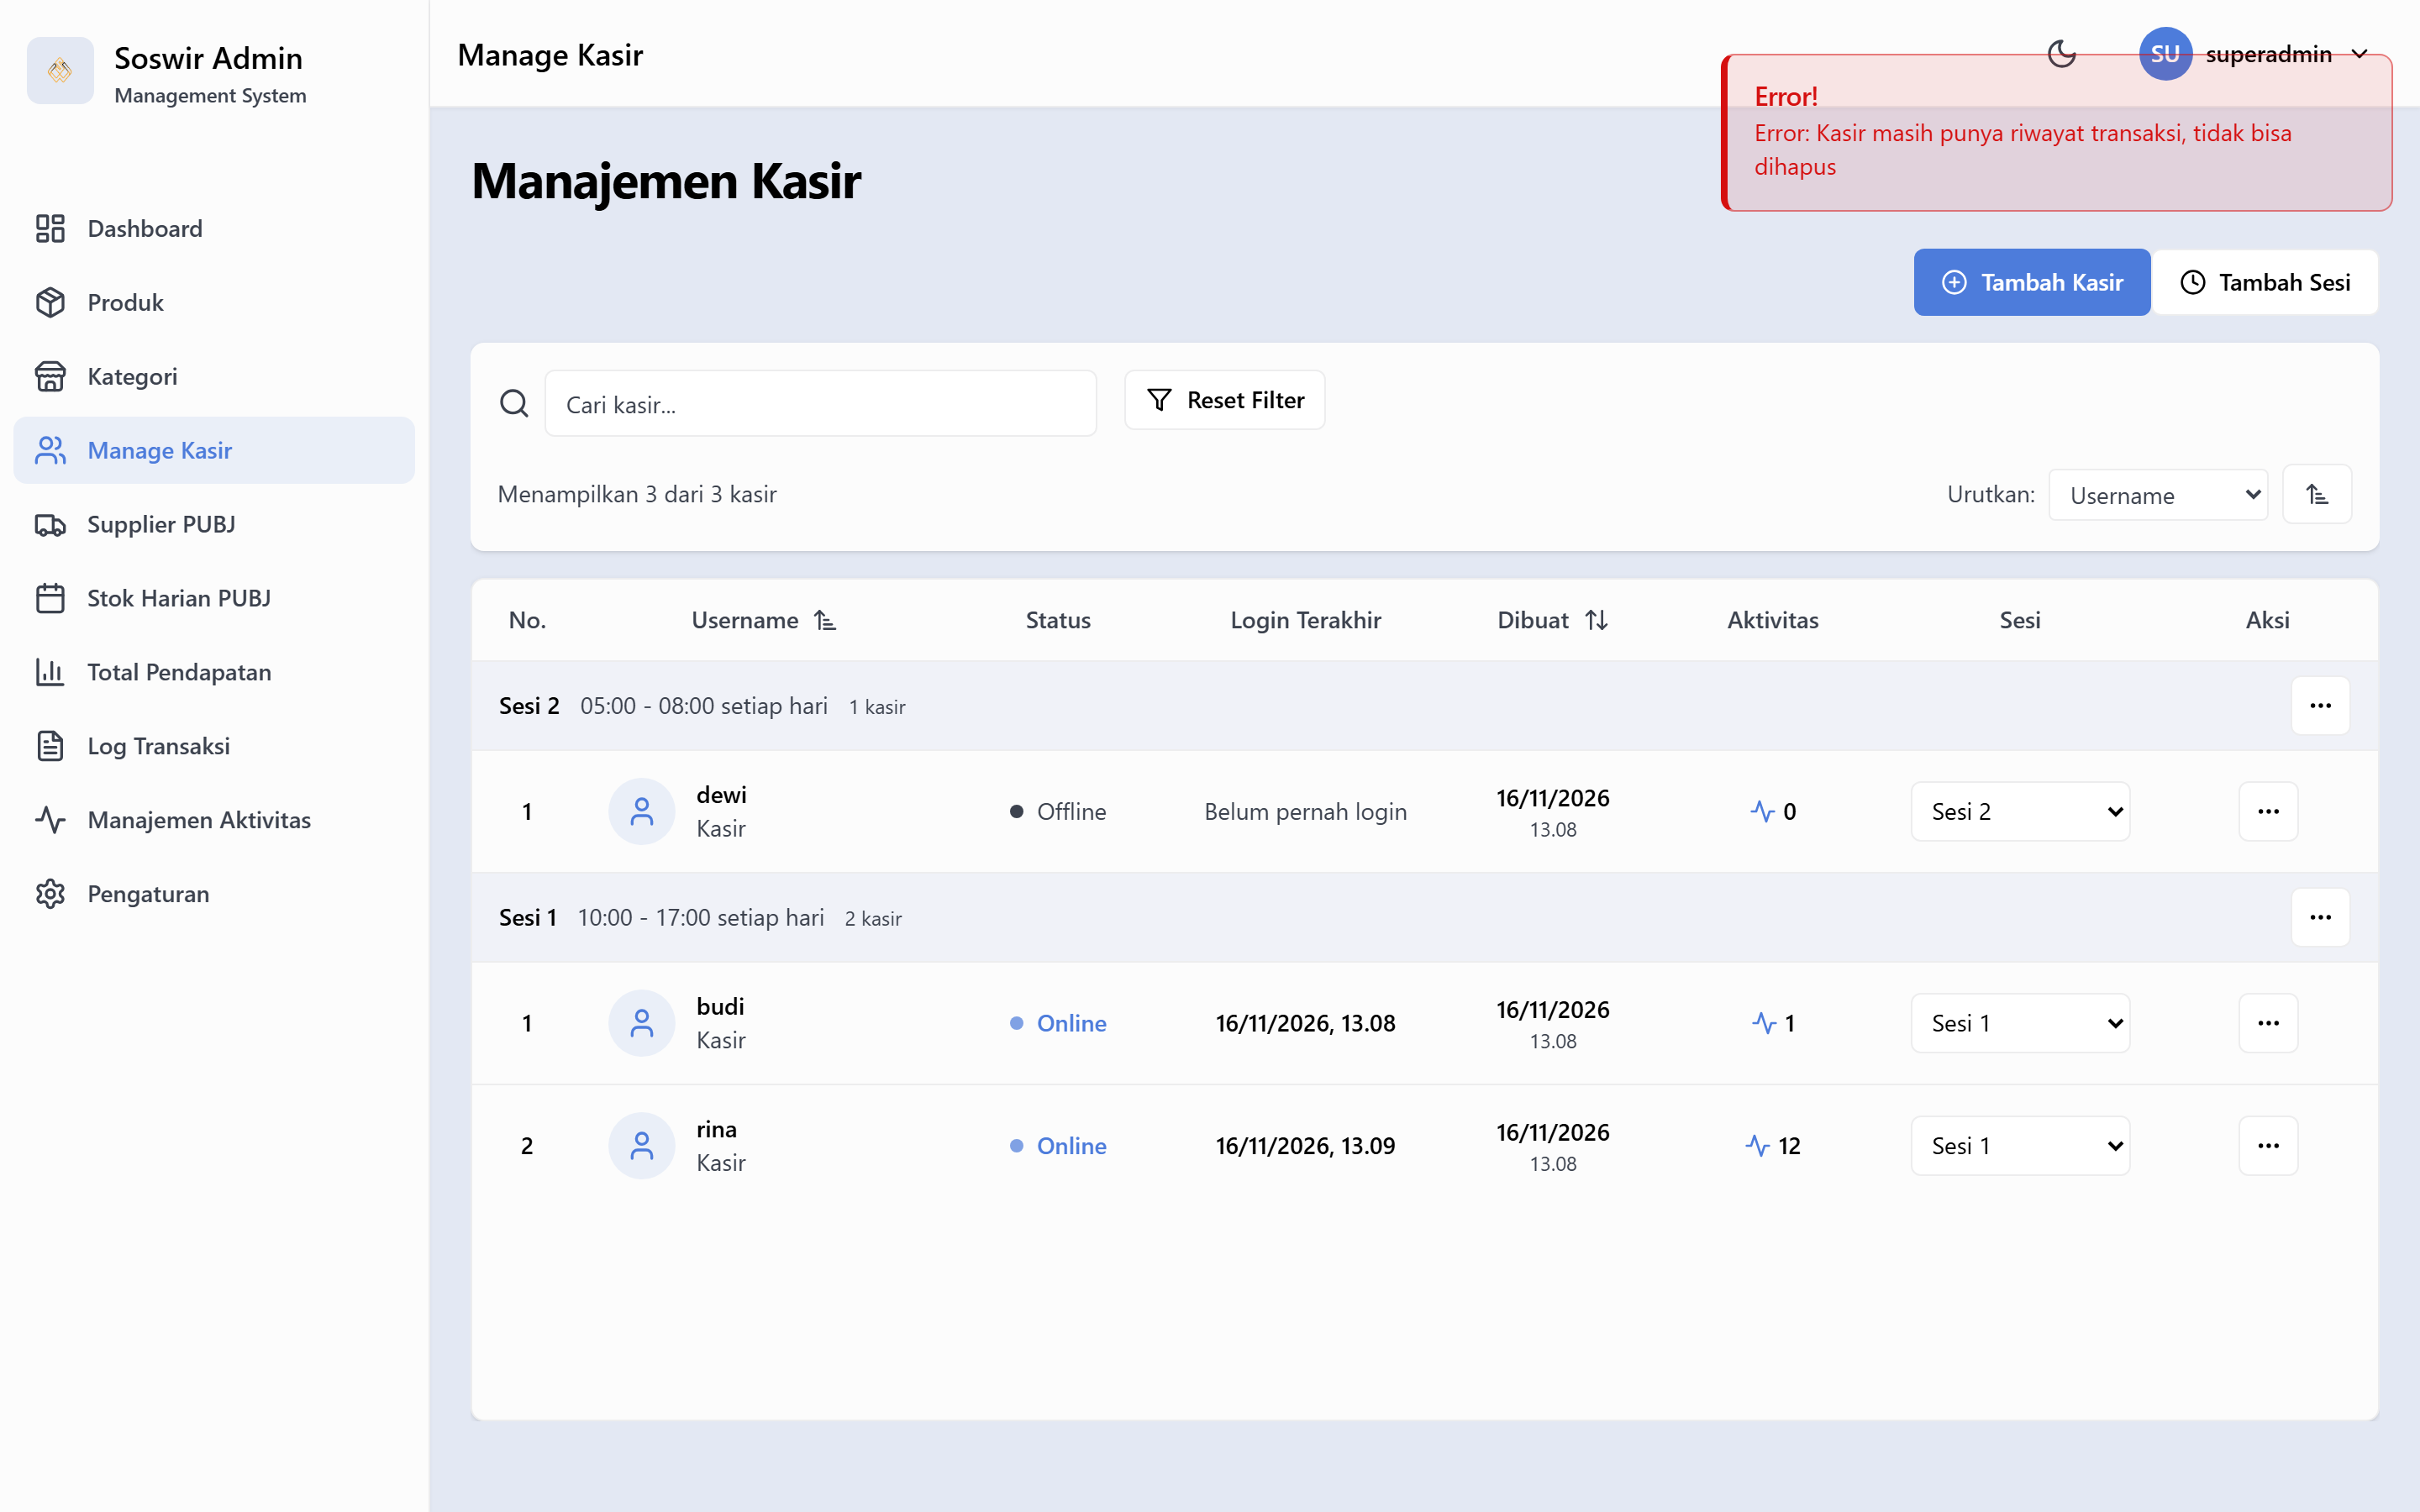
\includegraphics[width=0.99\linewidth,height=0.40\textheight,keepaspectratio,cfbox=garis 0.5pt 0pt]{img/38-kasir-hapus-ditolak.png}
\caption{Penghapusan kasir yang sudah punya transaksi ditolak.}
\end{figure}

% ---------------------------------------------------------------
\section{Laporan Pendapatan dan Transaksi}

\subsection{Total Pendapatan}

Menu \ui{Total Pendapatan} merangkum penjualan per hari, per bulan, dan per tahun.

\begin{figure}[H]
\centering
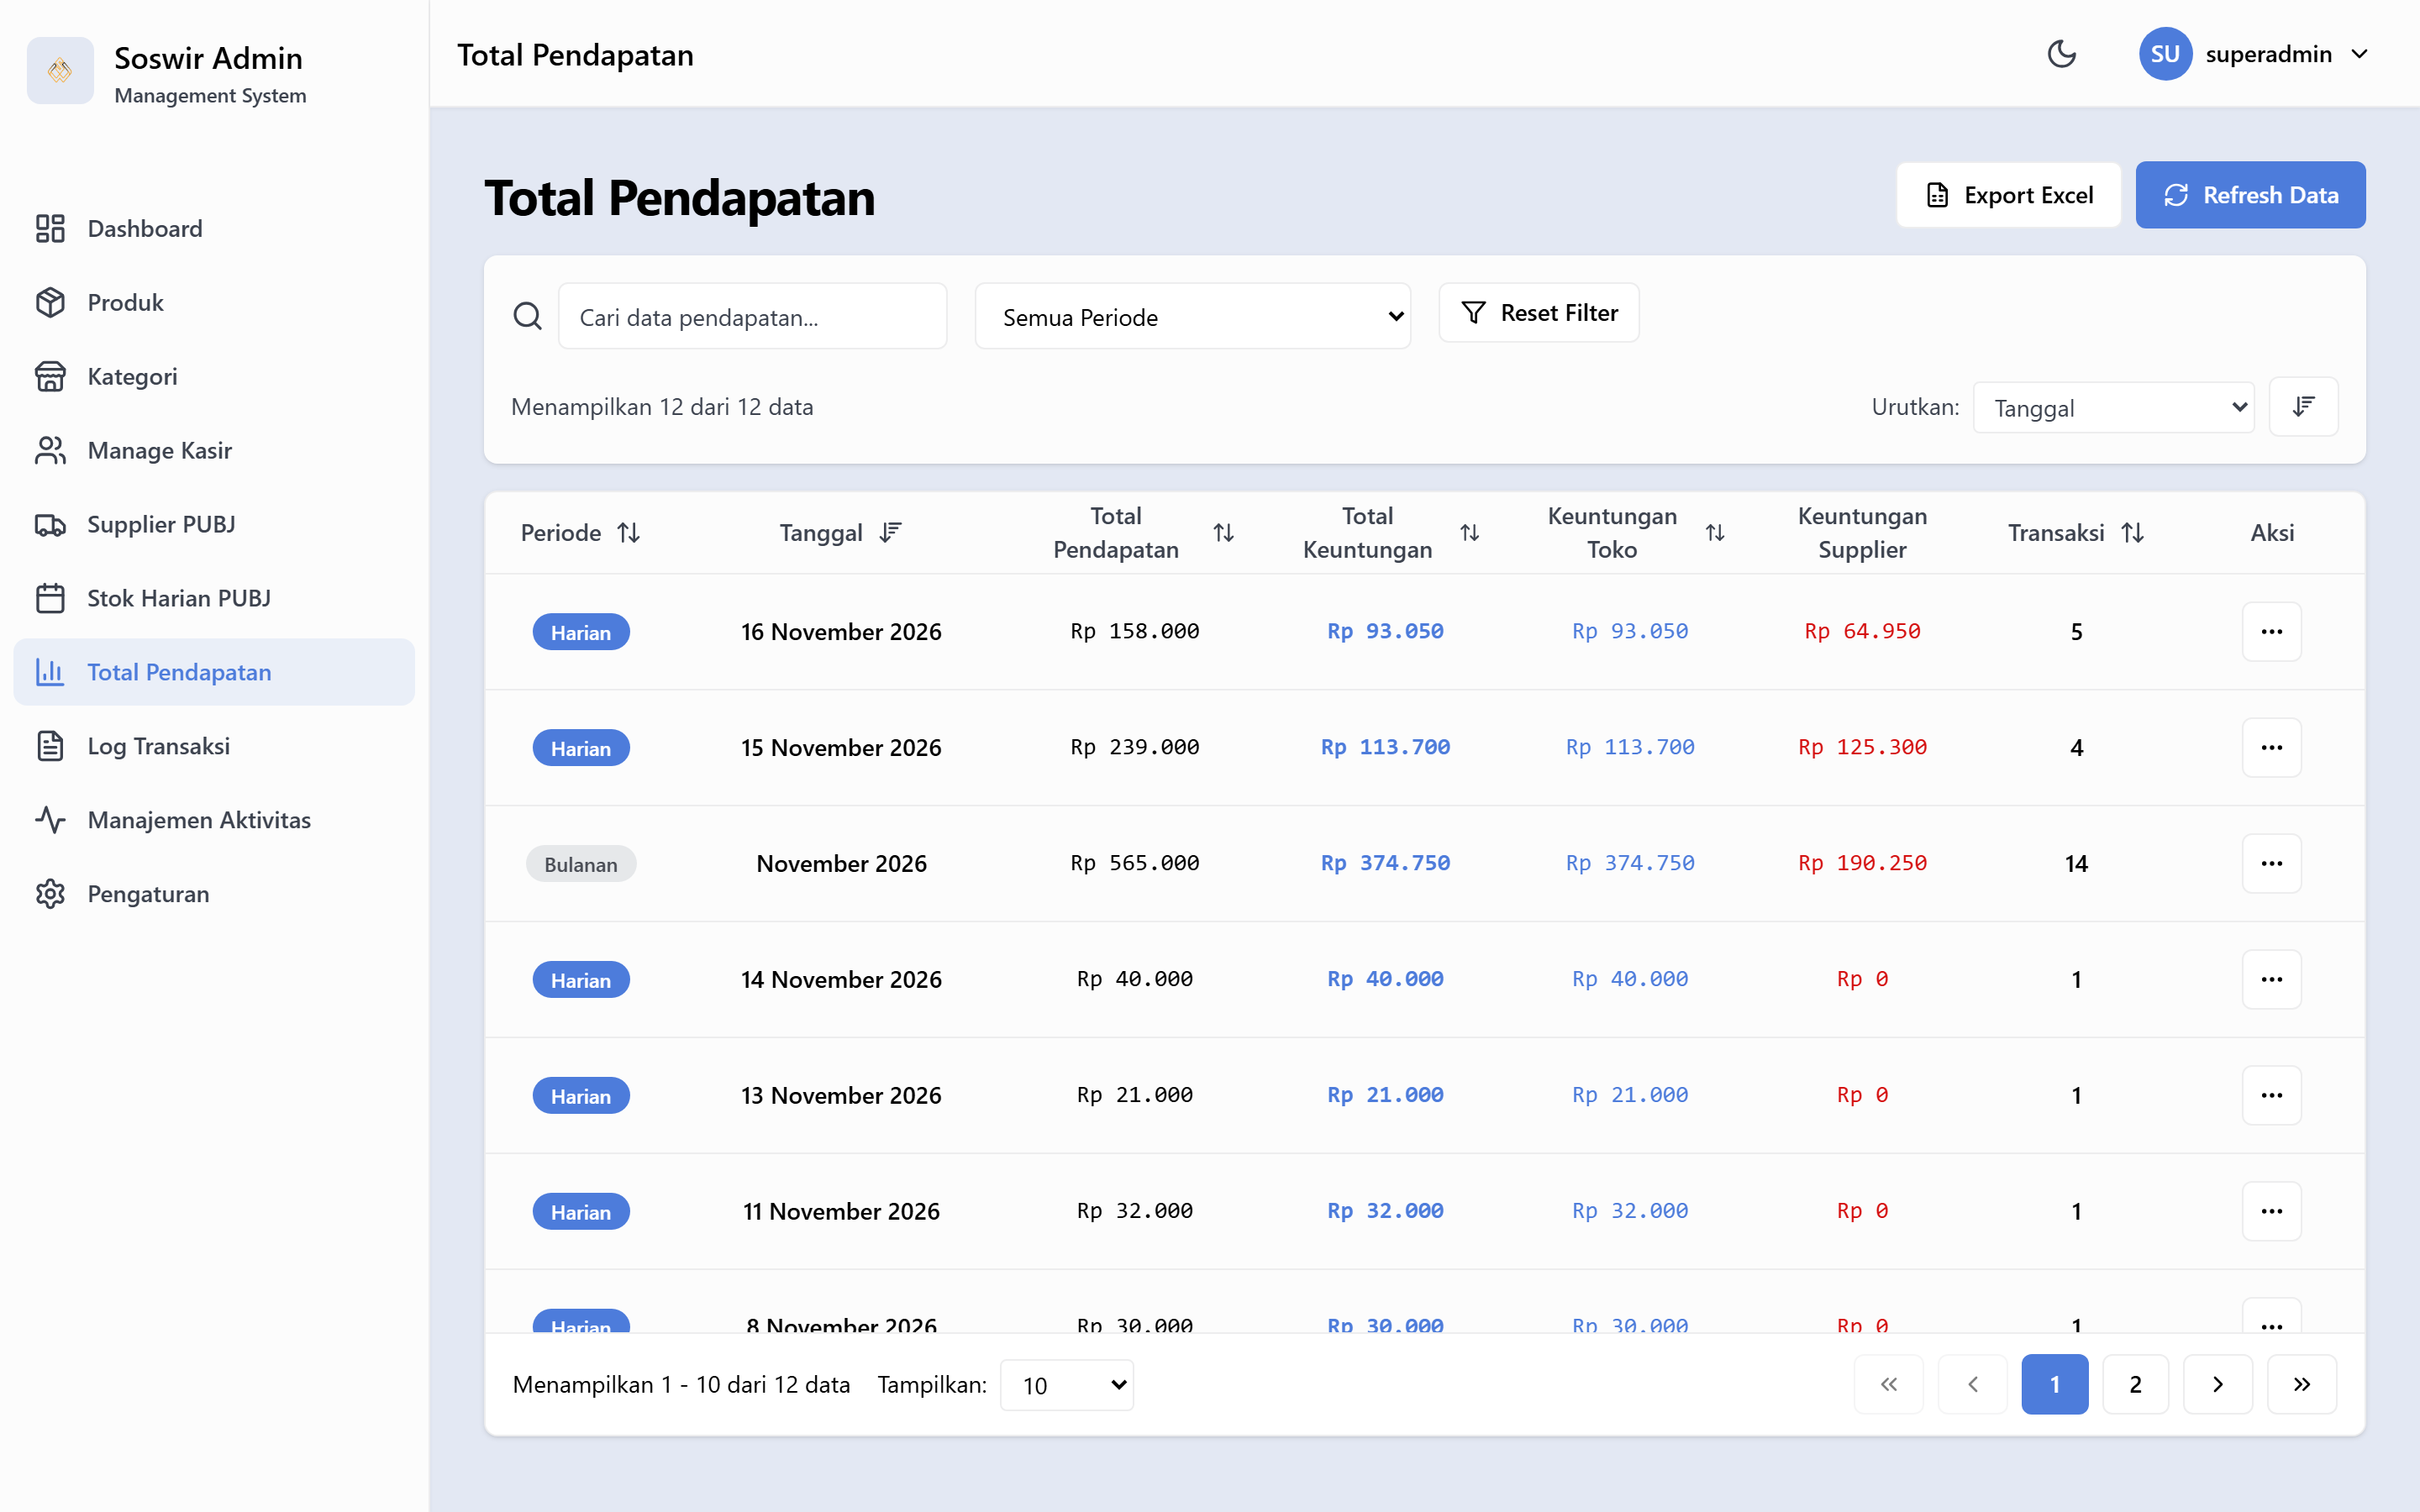
\includegraphics[width=0.99\linewidth,height=0.40\textheight,keepaspectratio,cfbox=garis 0.5pt 0pt]{img/39-pendapatan.png}
\caption{Halaman \ui{Total Pendapatan}.}
\end{figure}

\begin{itemize}
  \item \ui{Periode} menunjukkan jenis baris: \ui{Harian}, \ui{Bulanan}, atau \ui{Tahunan}. Pilih salah satunya di daftar \ui{Semua Periode} untuk menyaring.
  \item \ui{Total Pendapatan}: semua uang penjualan pada periode itu.
  \item \ui{Keuntungan Toko}: 100\% penjualan produk toko ditambah fee toko dari PUBJ. \ui{Total Keuntungan} menunjukkan angka yang sama.
  \item \ui{Keuntungan Supplier}: bagian supplier dari barang titipan.
  \item \ui{Transaksi}: jumlah transaksi pada periode itu.
\end{itemize}

Untuk melihat rincian satu periode, buka menu aksi baris tersebut lalu pilih \ui{Lihat Detail}. Jendela detail menampilkan setiap produk yang terjual beserta waktu, metode pembayaran, kasir, dan pembagian keuntungannya.

\begin{figure}[H]
\centering
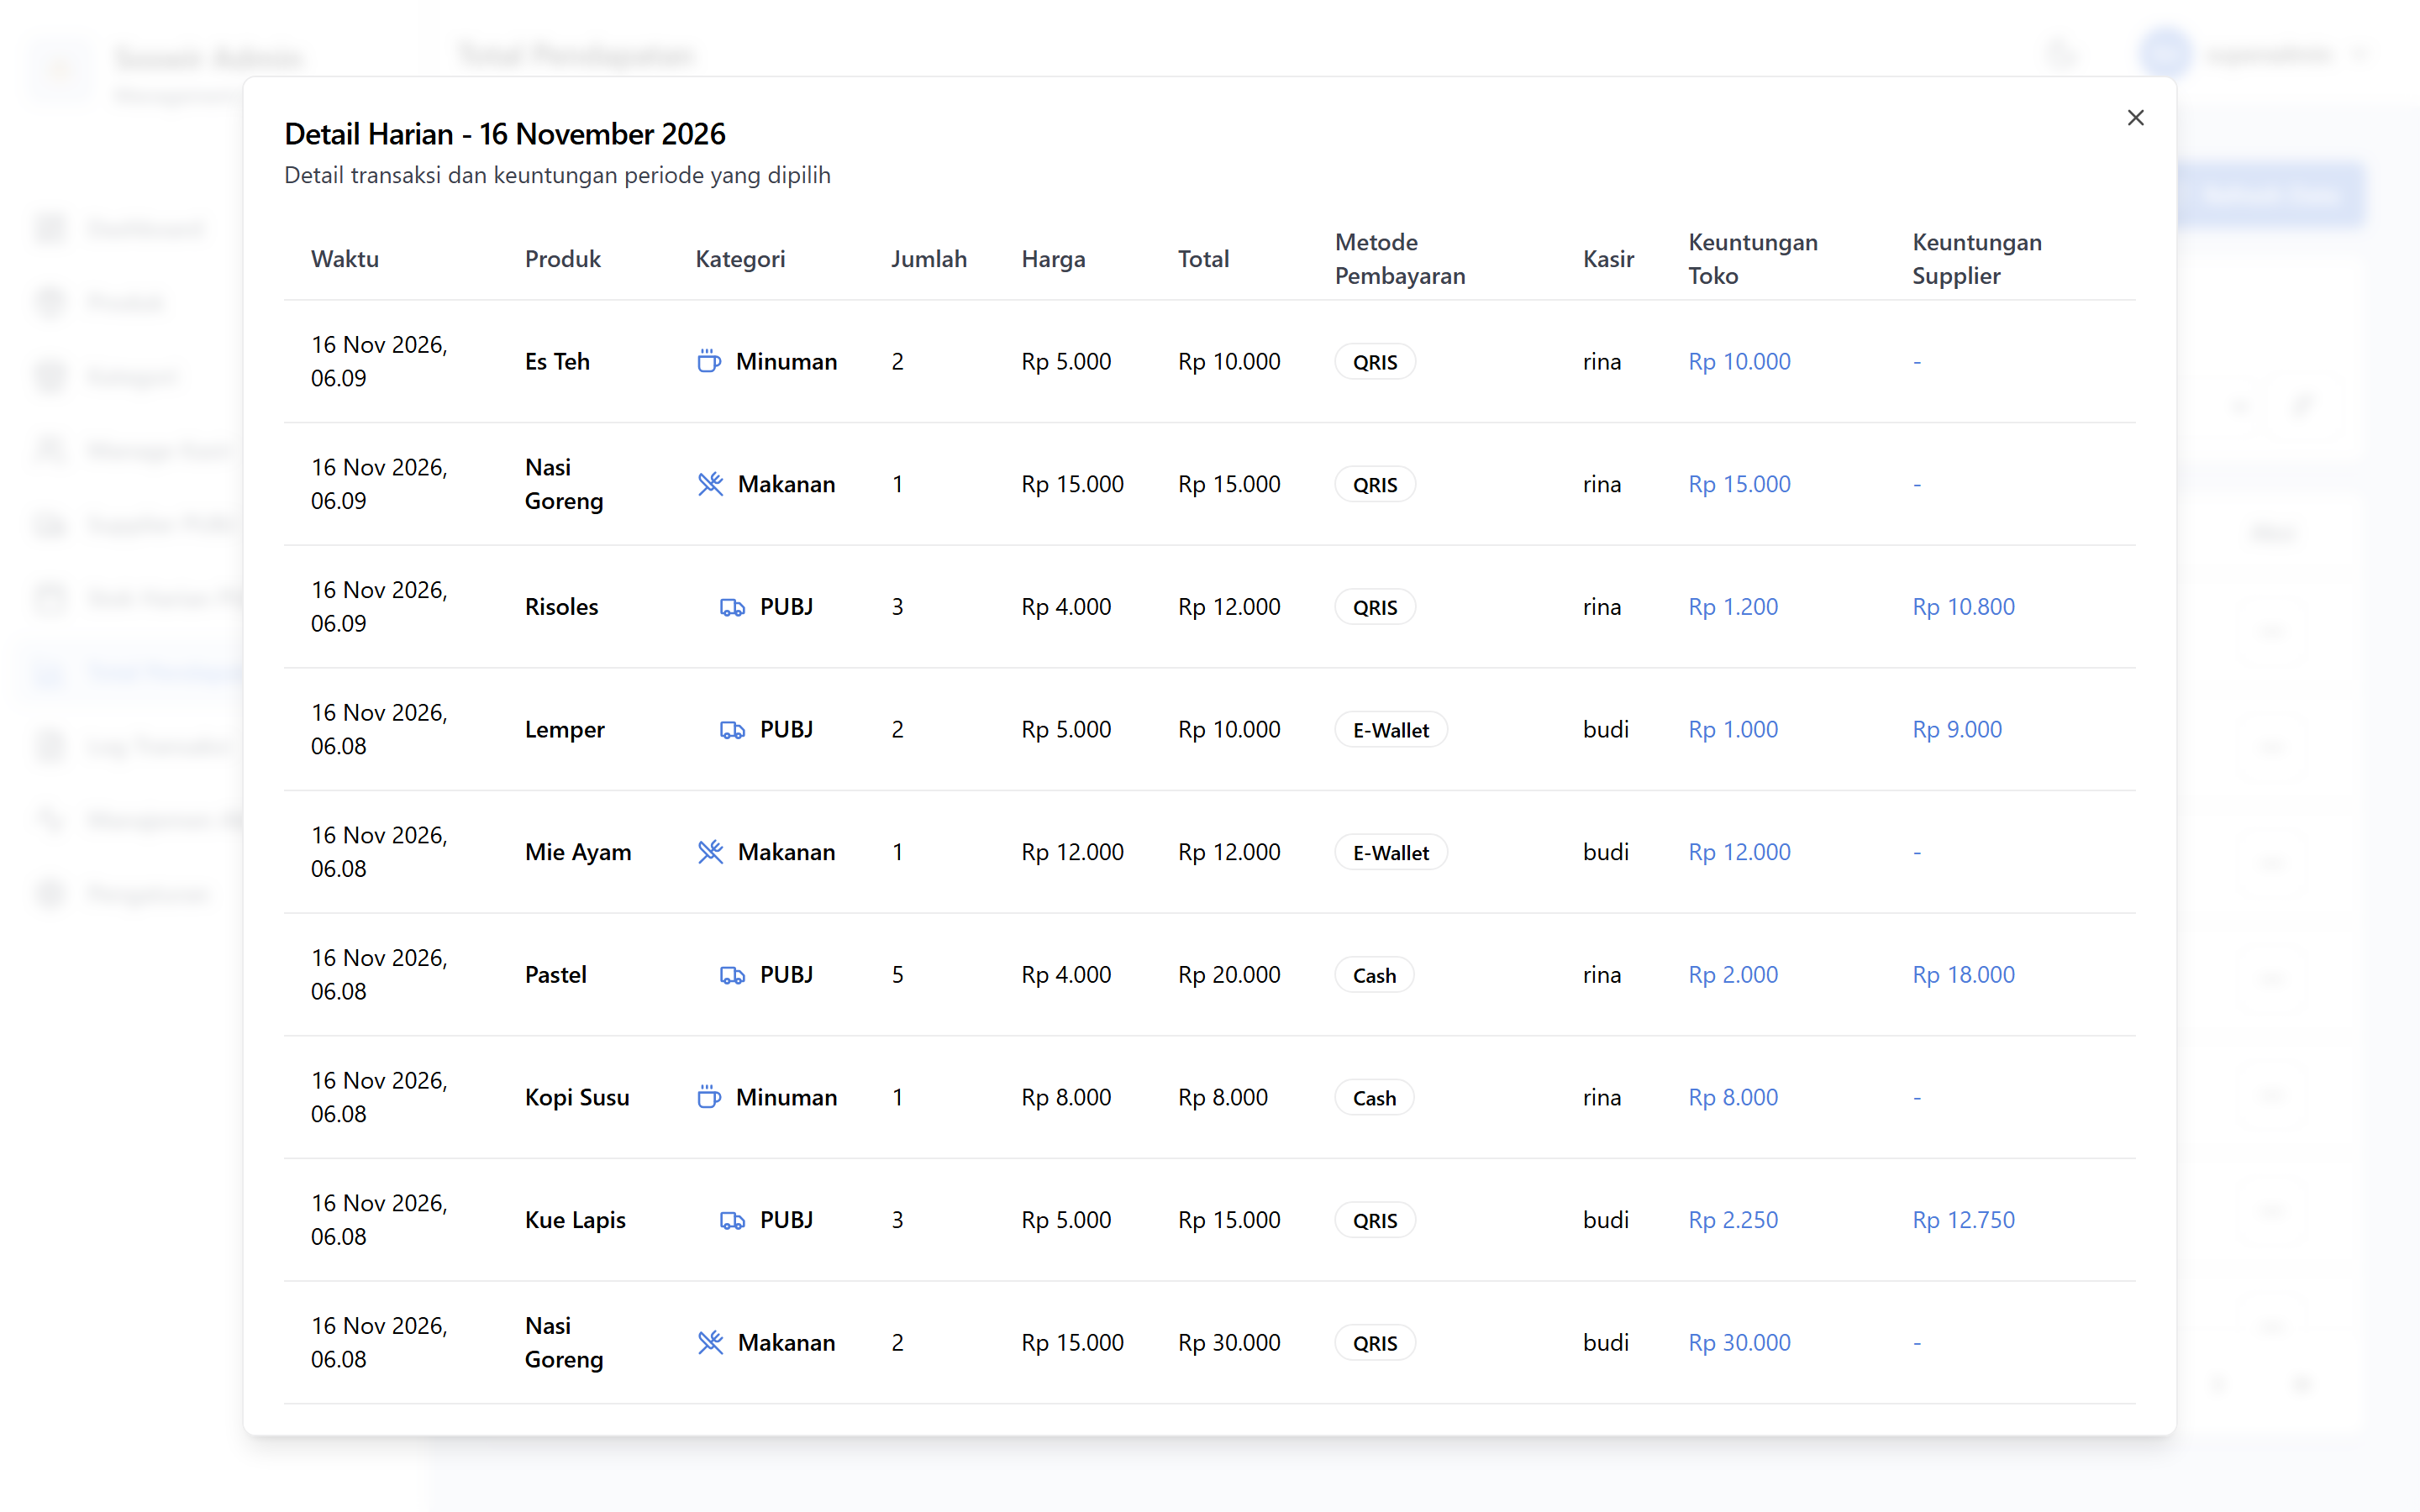
\includegraphics[width=0.99\linewidth,height=0.40\textheight,keepaspectratio,cfbox=garis 0.5pt 0pt]{img/40-pendapatan-detail.png}
\caption{Detail pendapatan harian.}
\end{figure}

\subsection{Ekspor Total Pendapatan ke Excel}

\begin{enumerate}
  \item Tekan \ui{Export Excel} di kanan atas halaman \ui{Total Pendapatan}.
  \item Pada \ui{Pilihan periode}, pilih \ui{Satu bulan}, \ui{Beberapa bulan}, atau \ui{Semua bulan}.
  \item Isi \ui{Bulan}, atau \ui{Bulan awal} dan \ui{Bulan akhir}.
  \item Tekan \ui{Export Excel}. File Excel terunduh ke komputer.
\end{enumerate}

\begin{figure}[H]
\centering
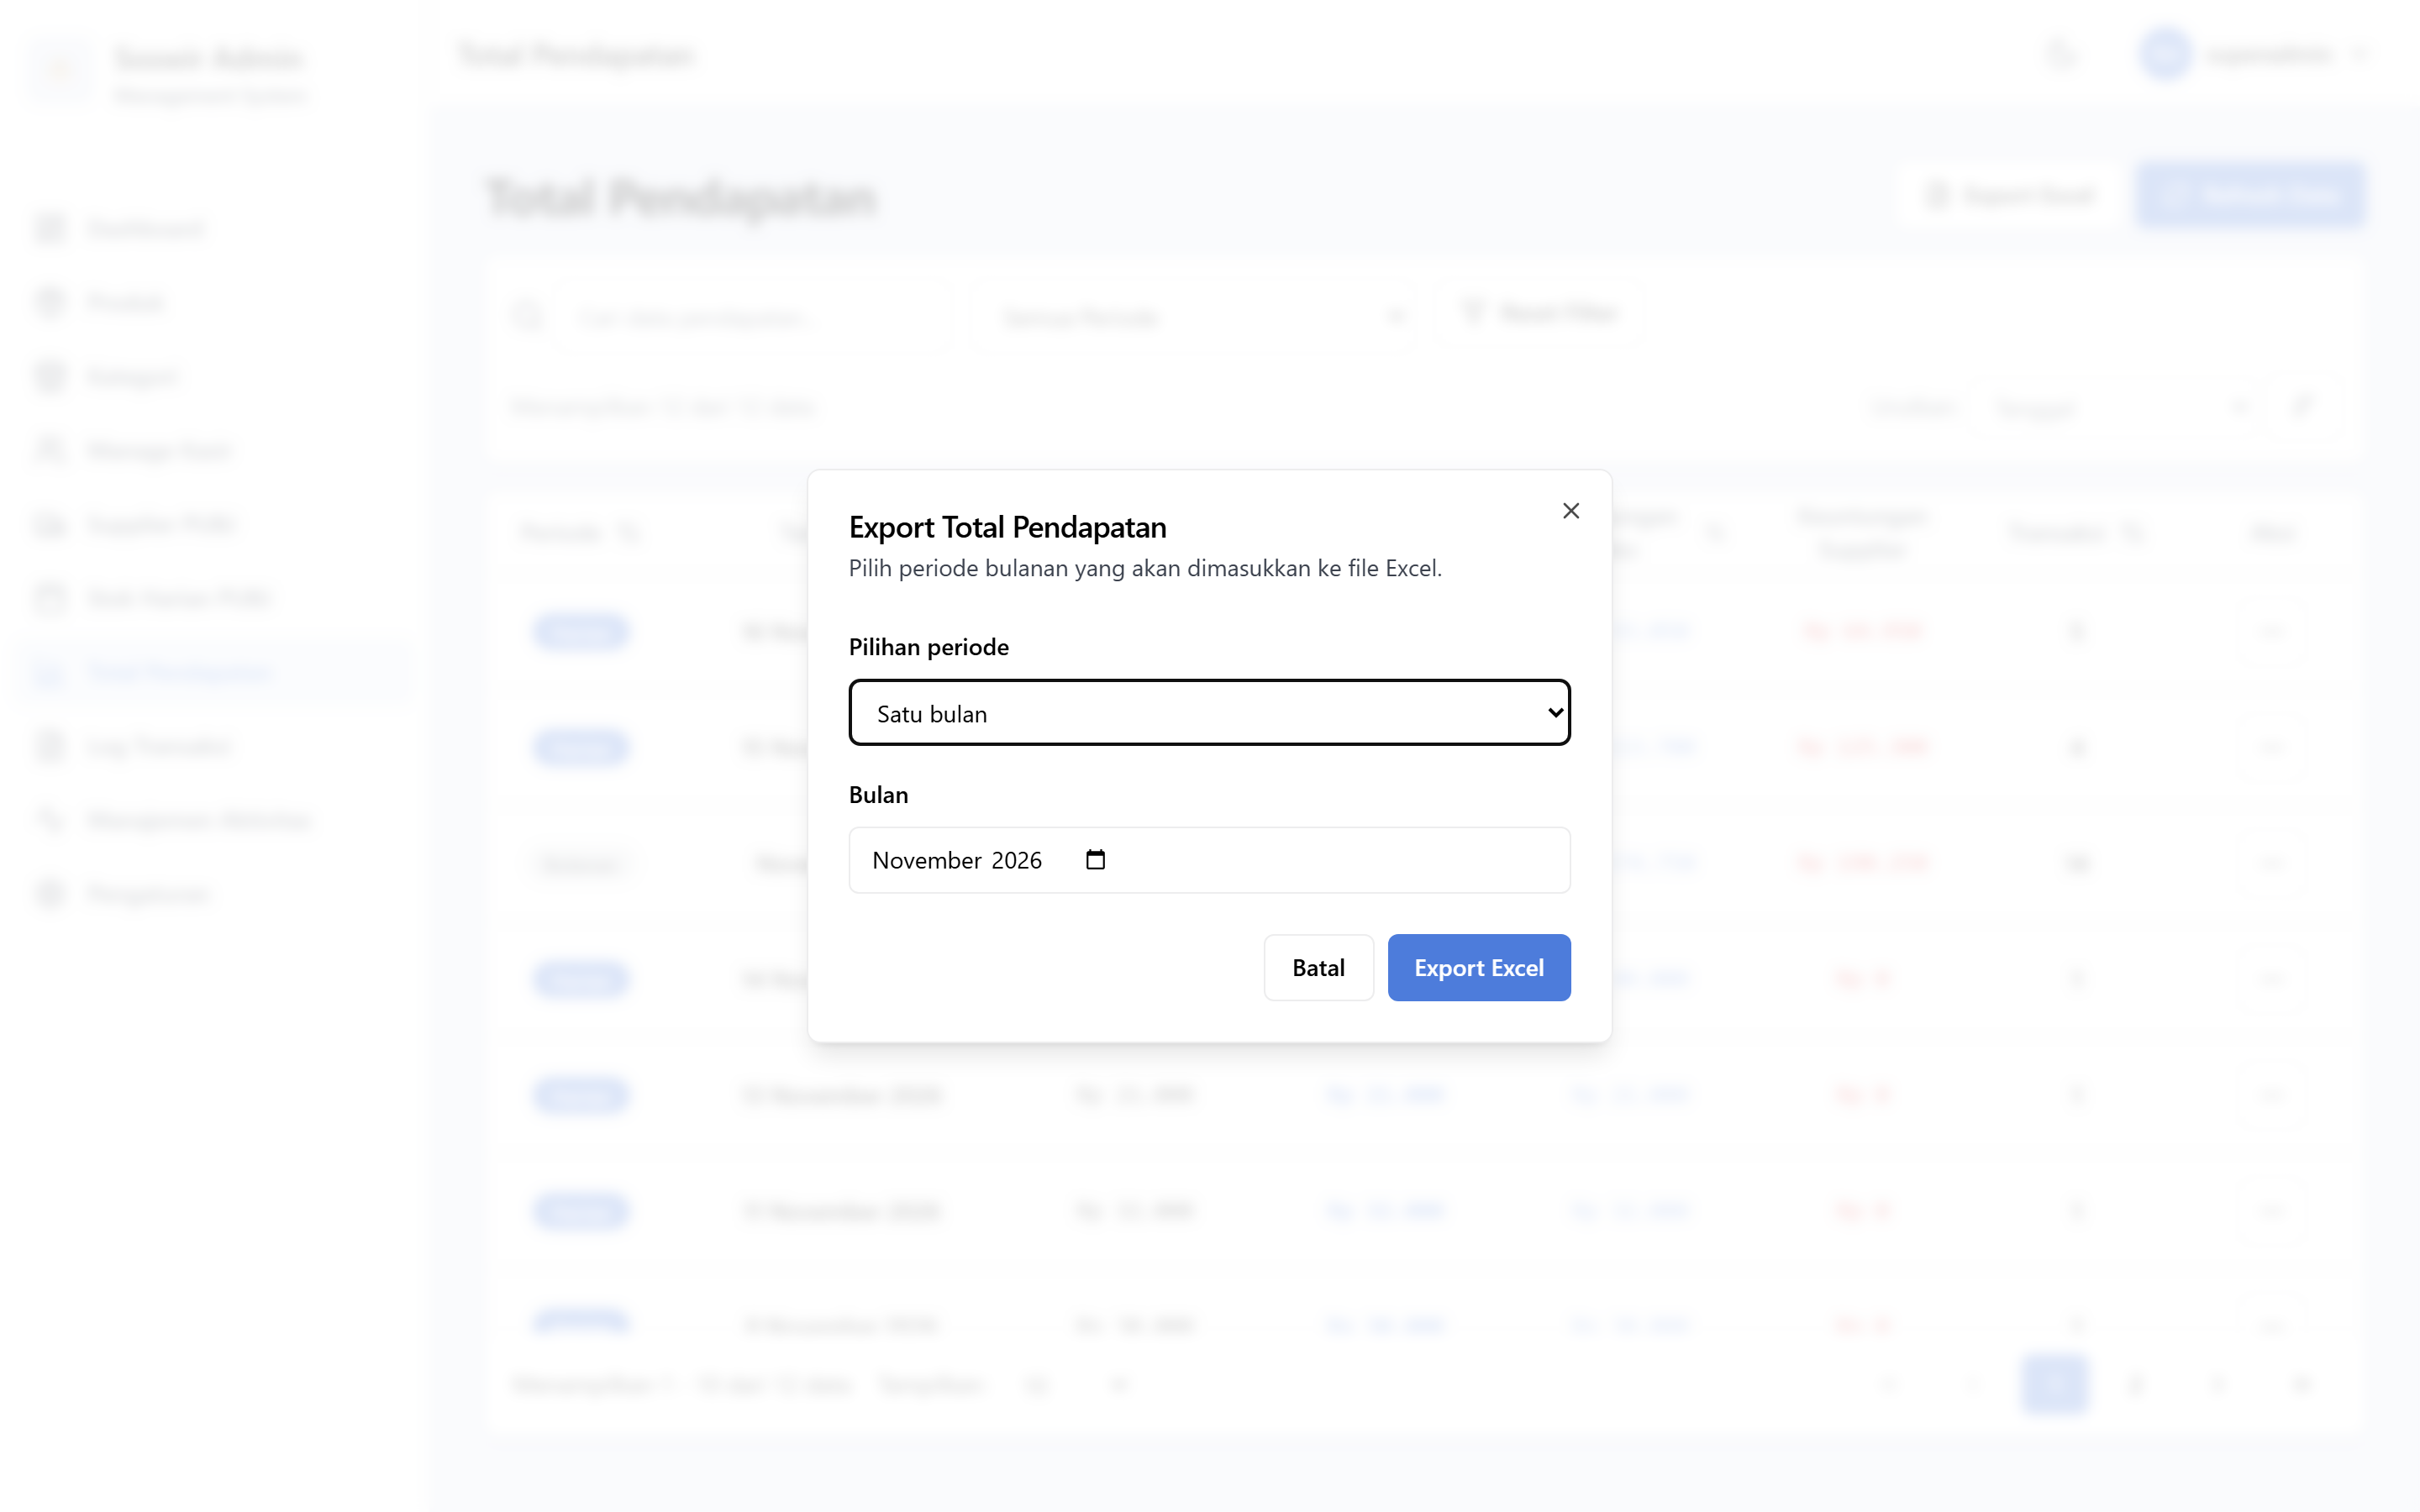
\includegraphics[width=0.99\linewidth,height=0.40\textheight,keepaspectratio,cfbox=garis 0.5pt 0pt]{img/41-pendapatan-ekspor.png}
\caption{Jendela \ui{Export Total Pendapatan}.}
\end{figure}

\subsection{Log Transaksi}

Menu \ui{Log Transaksi} berisi semua penjualan dari semua kasir. Satu baris adalah satu produk dalam satu transaksi, lengkap dengan kasir, metode pembayaran, \ui{Keuntungan Toko}, dan \ui{Keuntungan Supplier}.

\begin{enumerate}
  \item Cari lewat kotak \ui{Cari transaksi...}.
  \item Isi dua kotak tanggal untuk menampilkan transaksi dalam rentang tertentu. \ui{Reset} menghapus saringan.
  \item Atur urutan lewat \ui{Urutkan:}, misalnya berdasarkan \ui{Kasir} atau \ui{Total}.
\end{enumerate}

\begin{figure}[H]
\centering
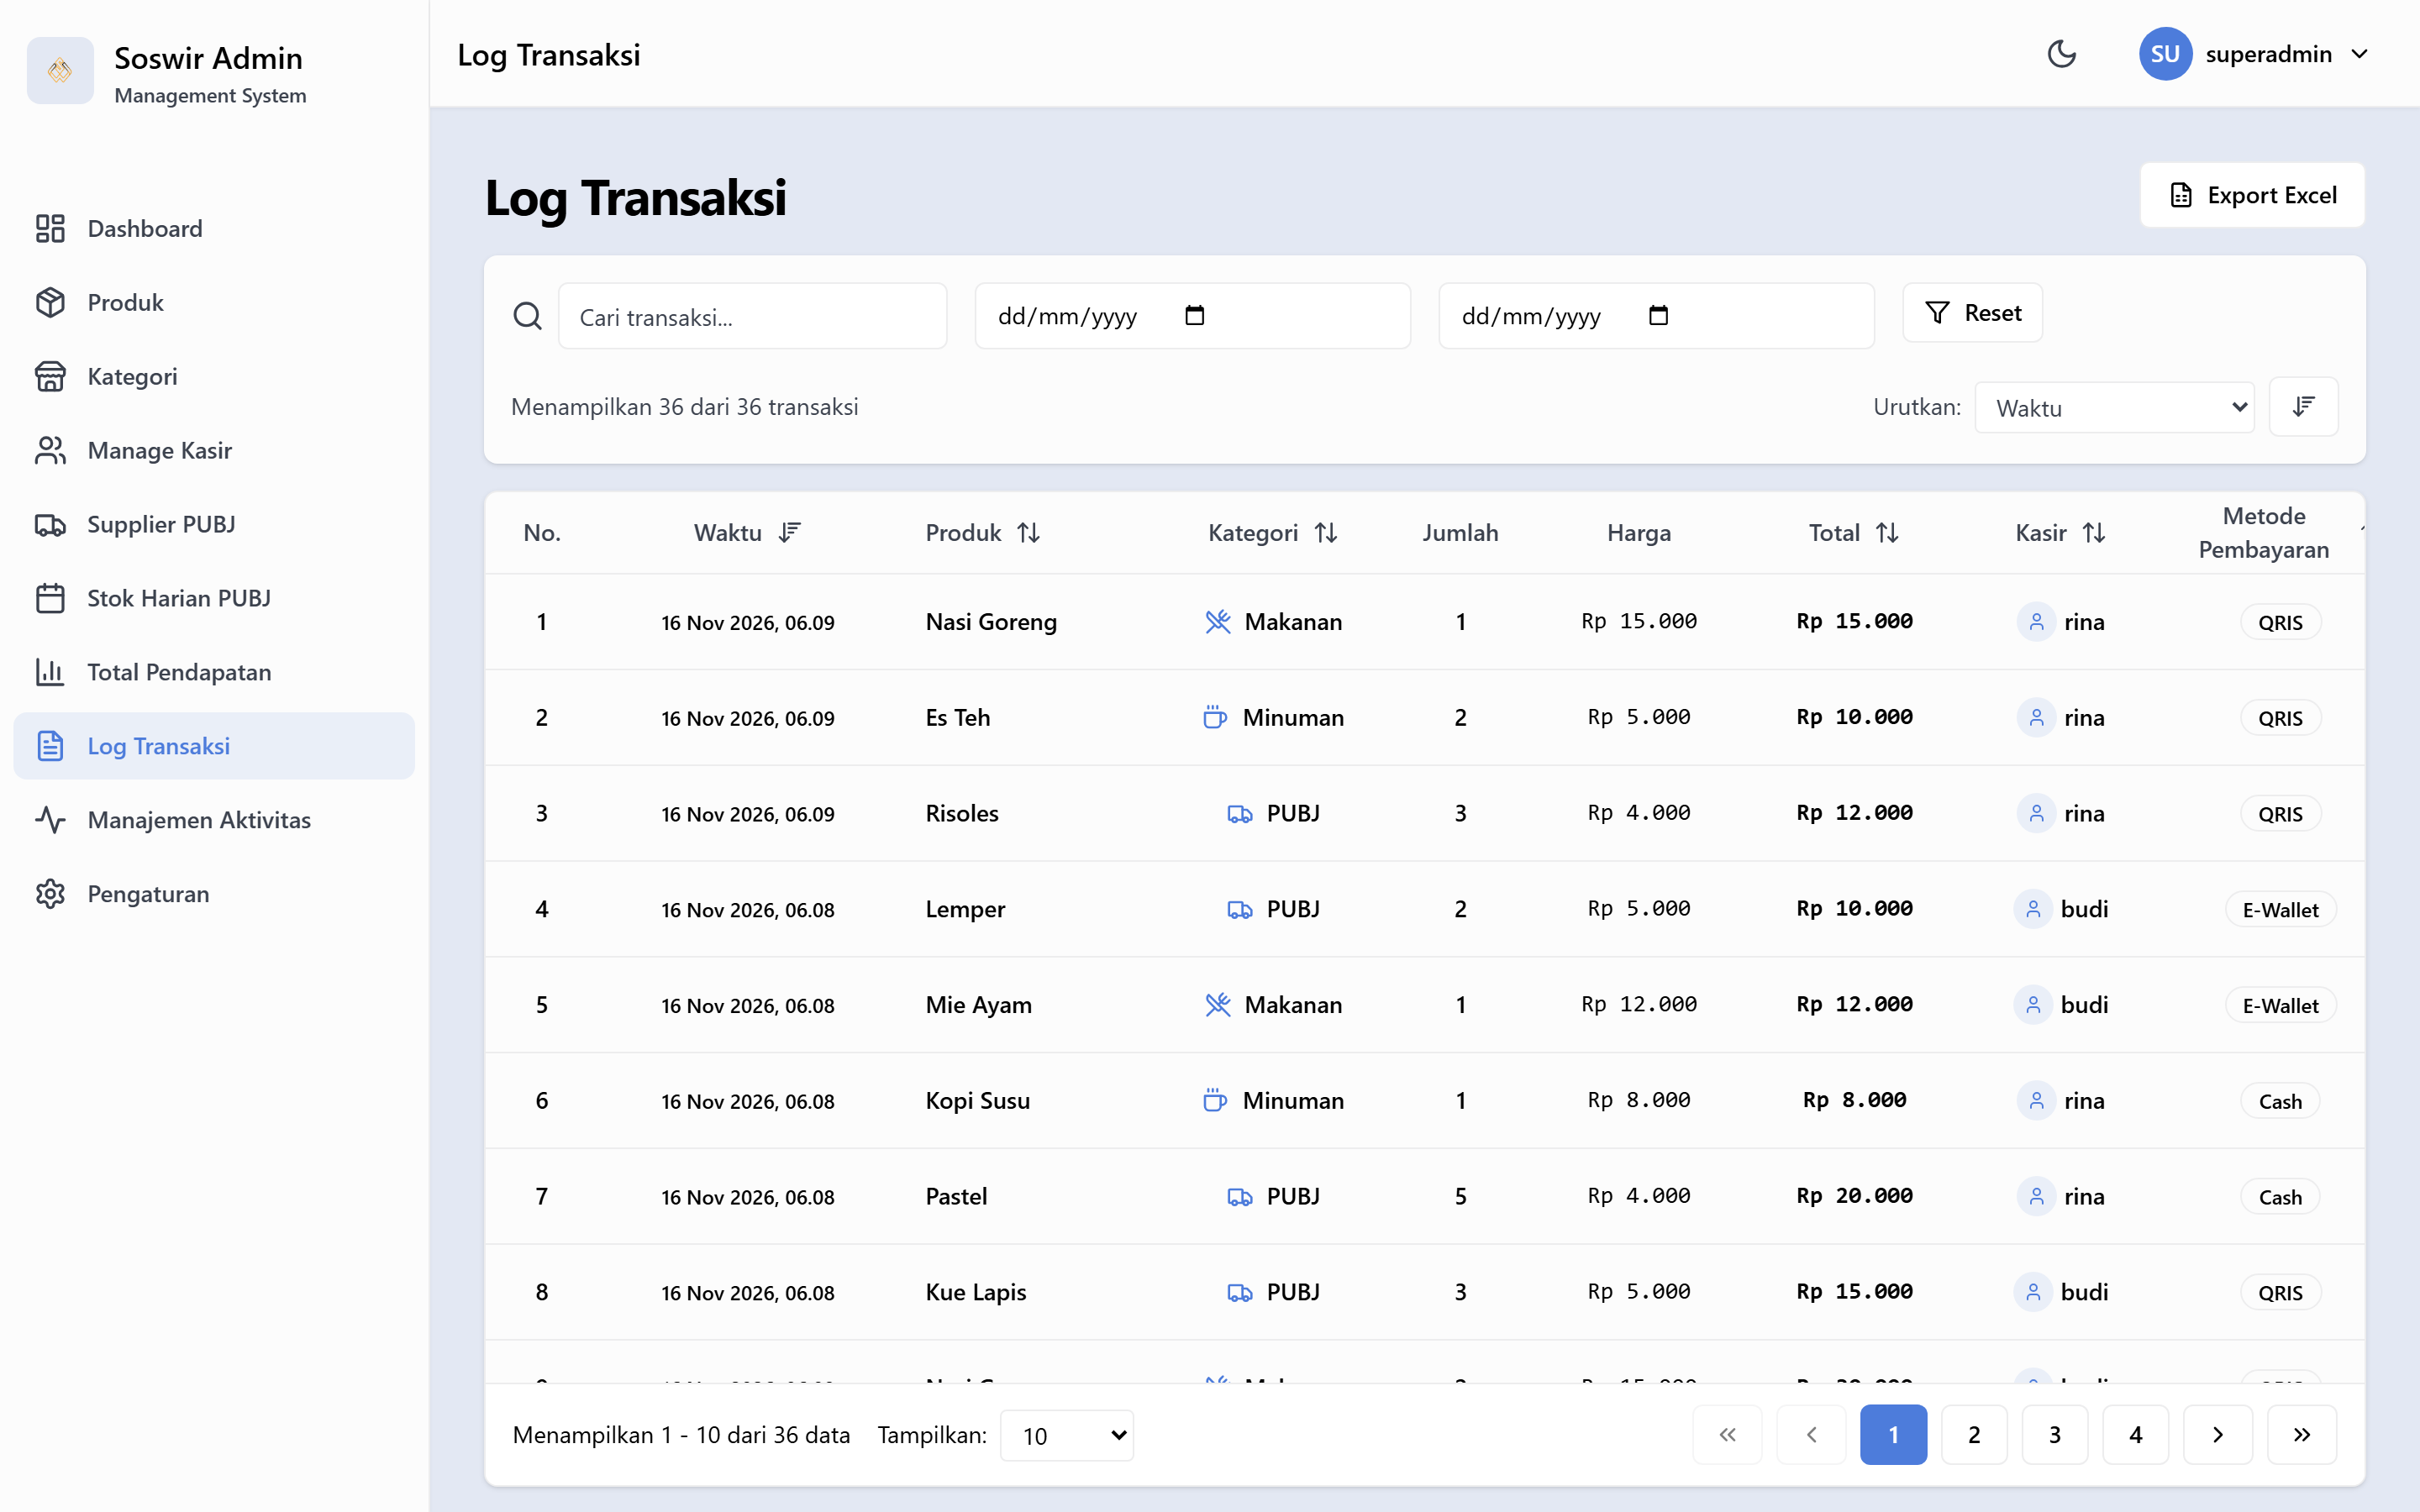
\includegraphics[width=0.99\linewidth,height=0.40\textheight,keepaspectratio,cfbox=garis 0.5pt 0pt]{img/42-log-transaksi.png}
\caption{Halaman \ui{Log Transaksi}.}
\end{figure}

\subsection{Ekspor Log Transaksi ke Excel}

\begin{enumerate}
  \item Tekan \ui{Export Excel} di halaman \ui{Log Transaksi}.
  \item Pilih \ui{Jenis laporan}: \ui{Rekap produk bulanan} (satu baris per produk per bulan) atau \ui{Detail per transaksi} (satu baris per produk dalam transaksi).
  \item Pilih \ui{Pilihan periode} dan bulannya, lalu tekan \ui{Export Excel}.
\end{enumerate}

\begin{figure}[H]
\centering
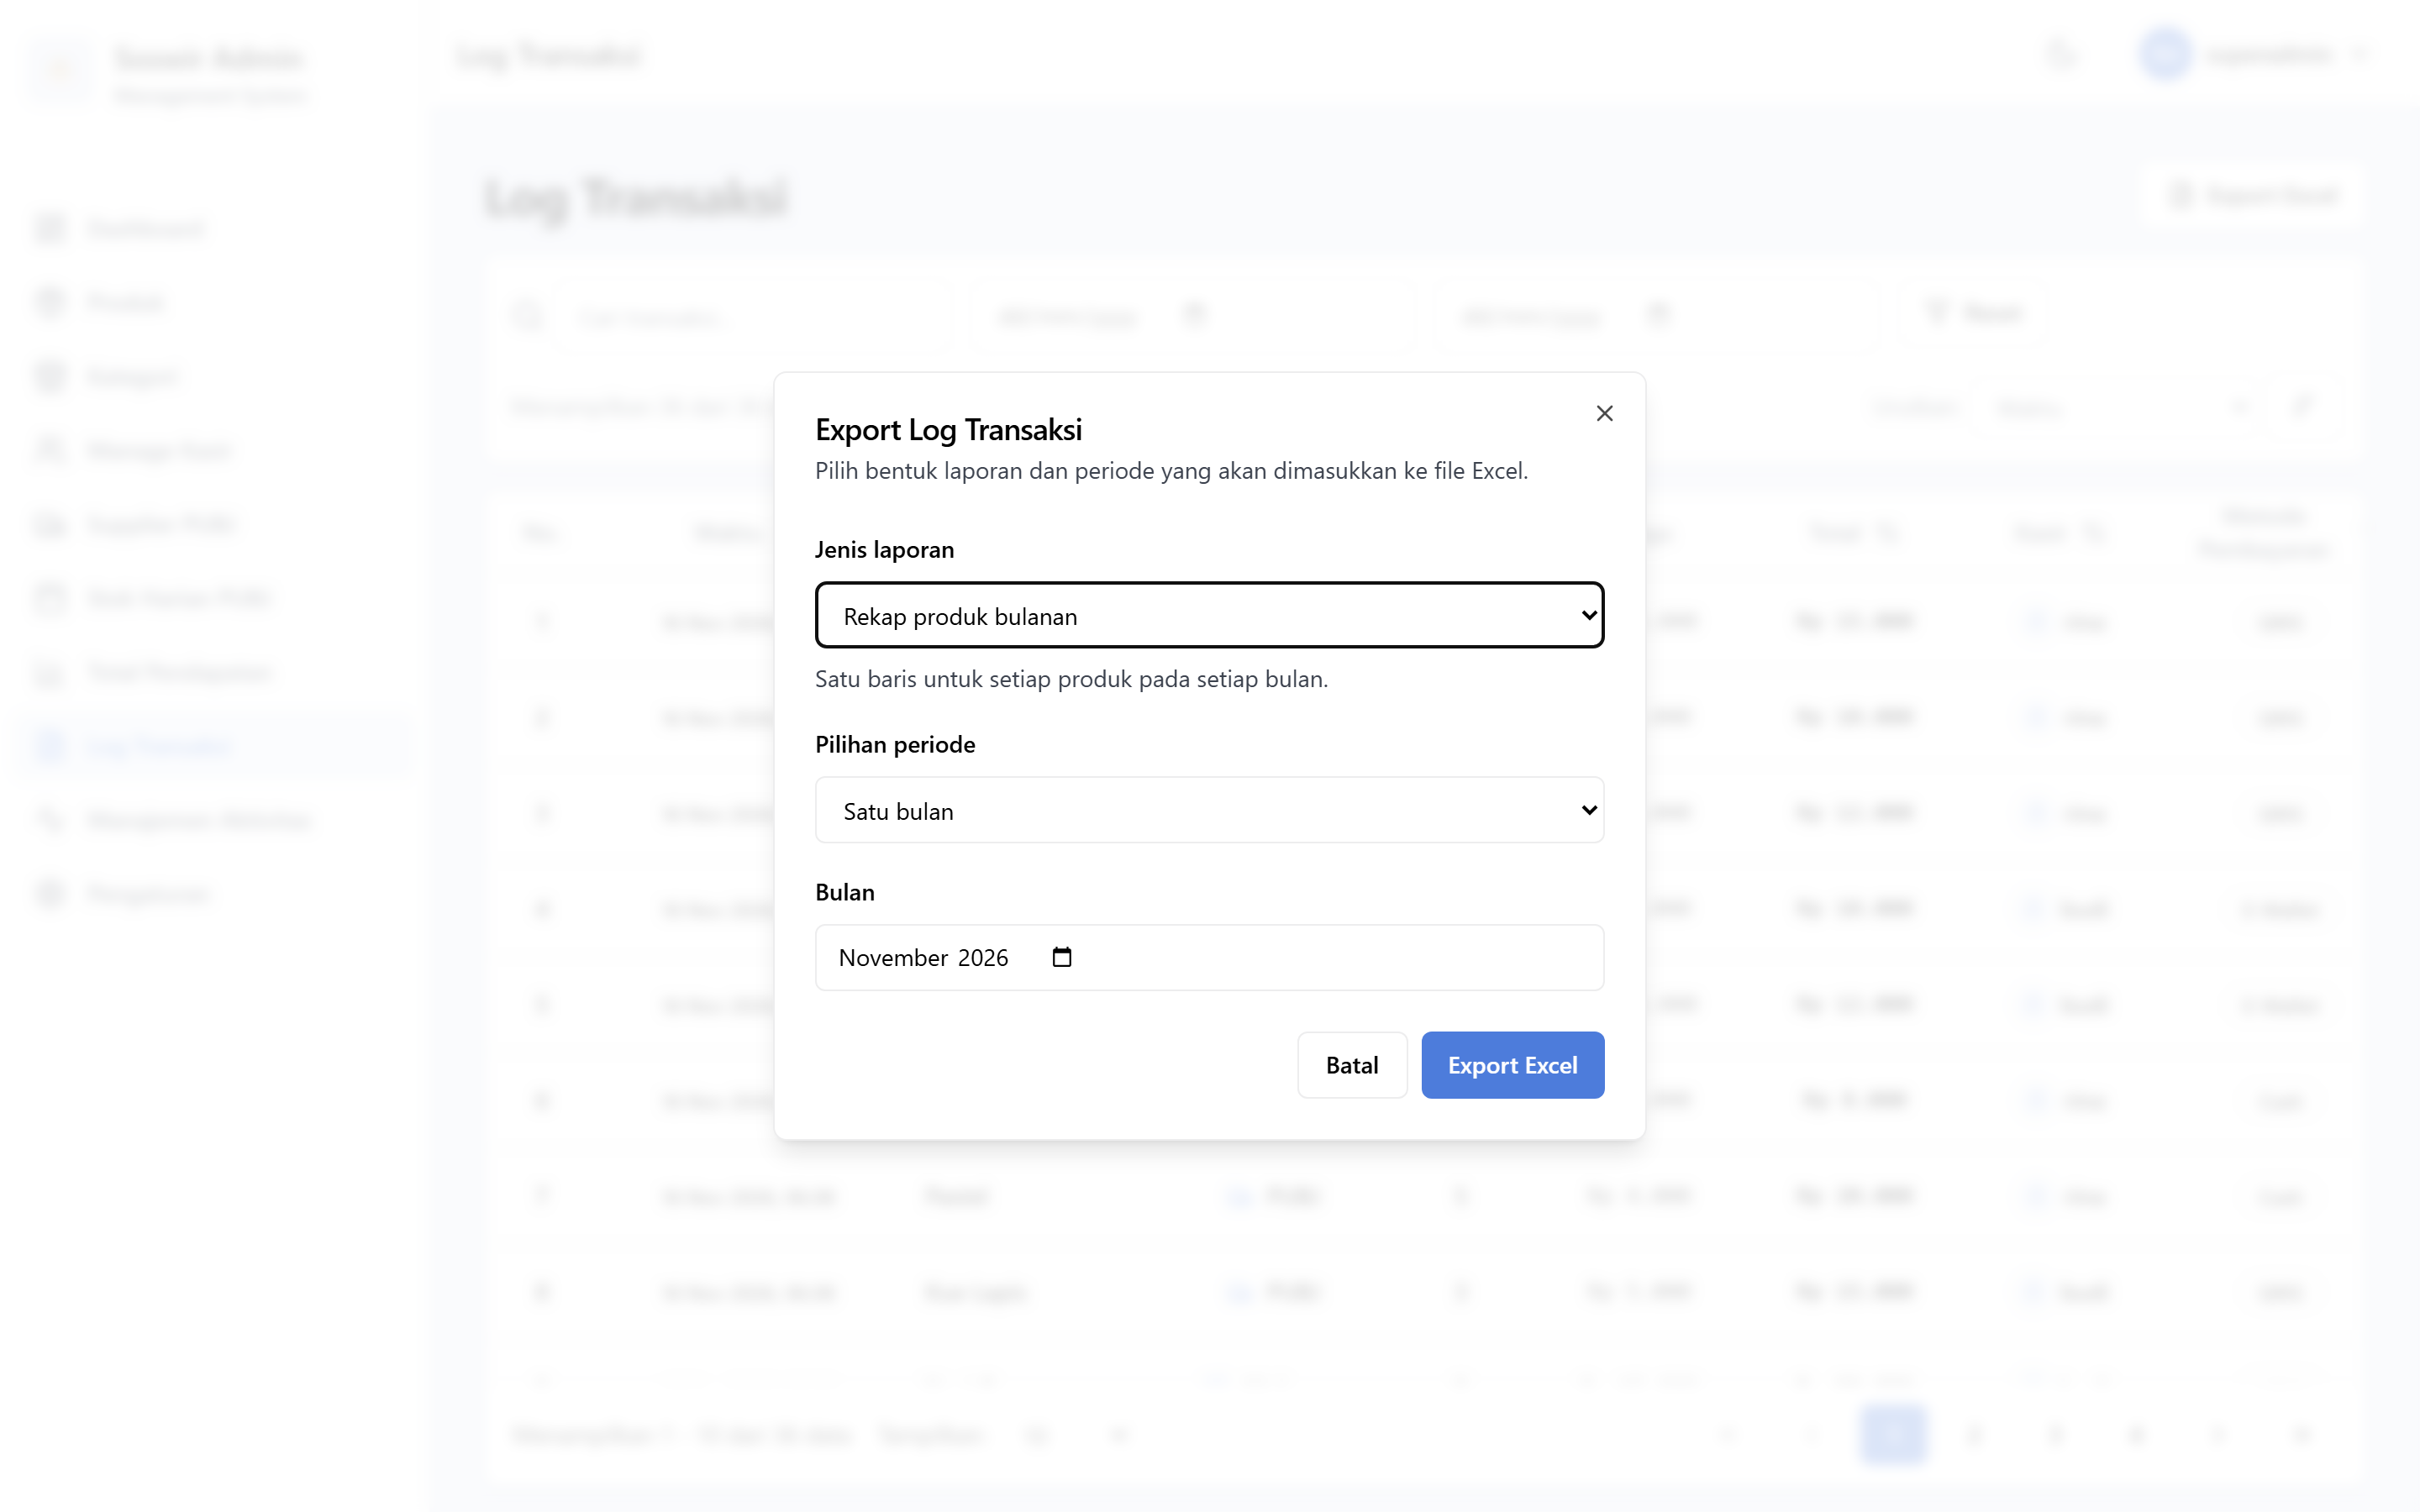
\includegraphics[width=0.99\linewidth,height=0.40\textheight,keepaspectratio,cfbox=garis 0.5pt 0pt]{img/43-log-transaksi-ekspor.png}
\caption{Jendela \ui{Export Log Transaksi}.}
\end{figure}

% ---------------------------------------------------------------
\section{Aktivitas dan Pengaturan}

\subsection{Manajemen Aktivitas}

Aplikasi mencatat aktivitas pengguna: masuk, keluar, dan halaman yang dibuka. Riwayat per kasir dilihat lewat \ui{Lihat Aktivitas} di \ui{Manage Kasir}. Halaman \ui{Manajemen Aktivitas} mengatur pembersihan catatan lama supaya data tidak menumpuk.

\begin{figure}[H]
\centering
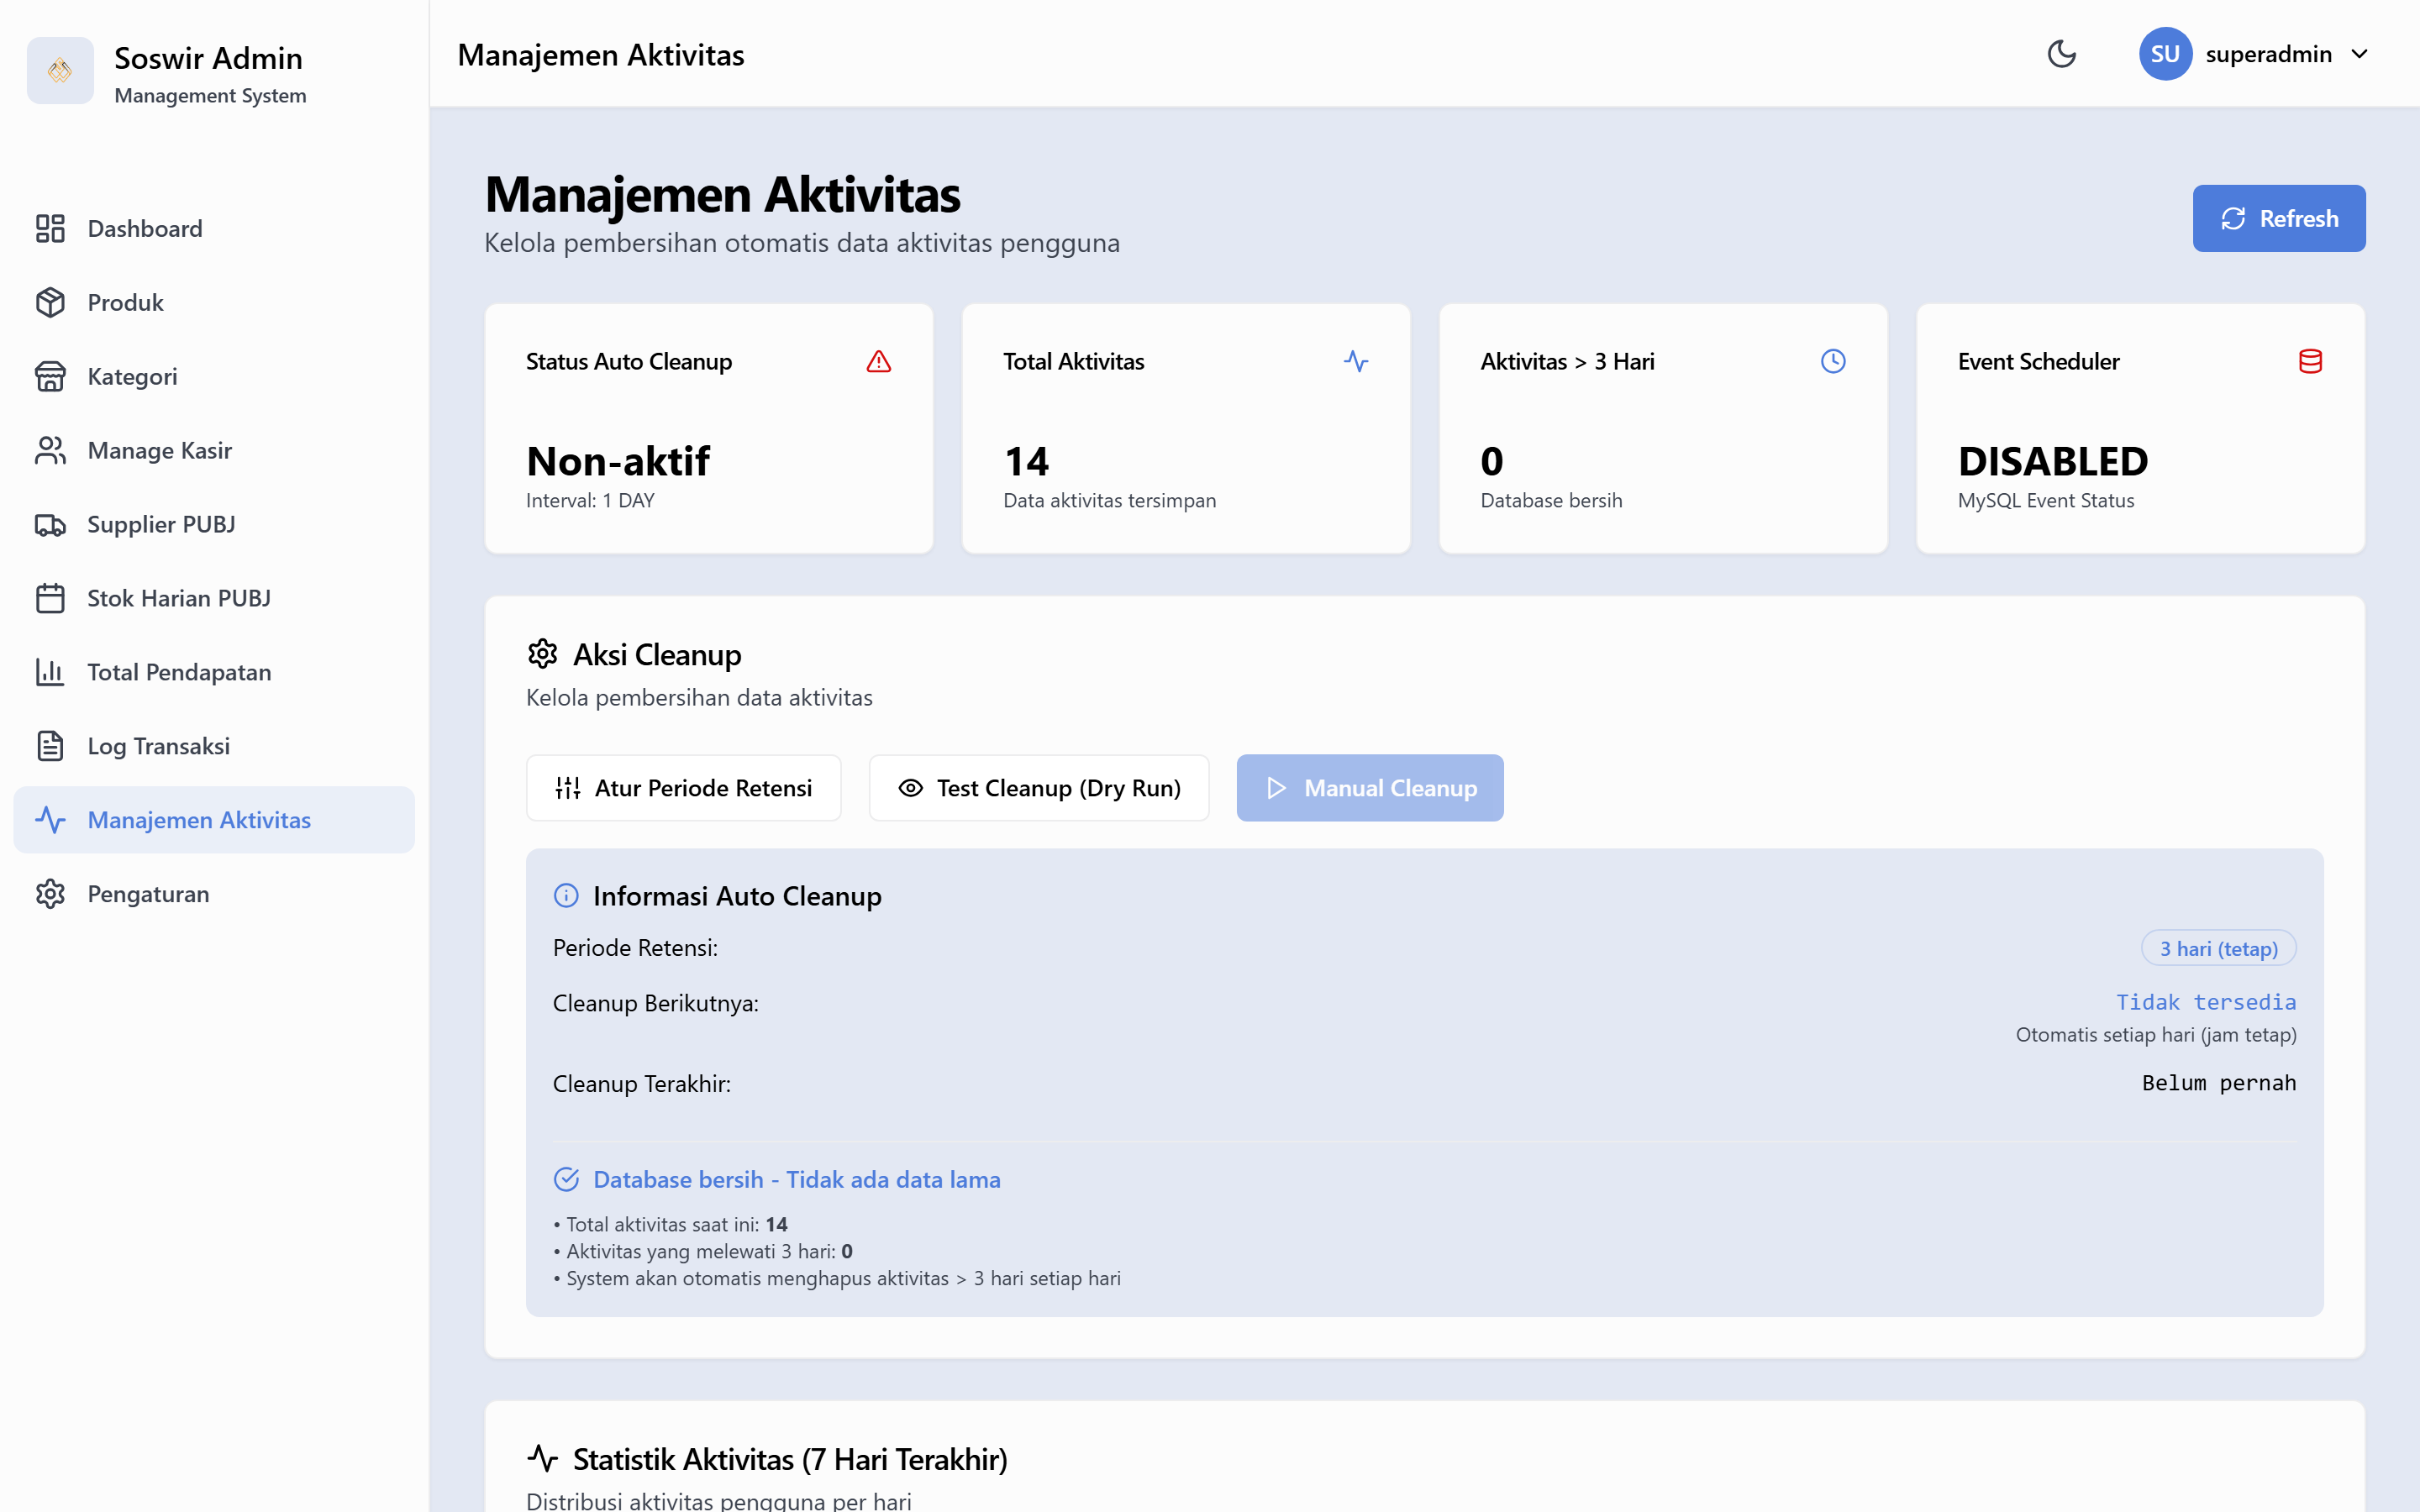
\includegraphics[width=0.99\linewidth,height=0.40\textheight,keepaspectratio,cfbox=garis 0.5pt 0pt]{img/44-aktivitas.png}
\caption{Halaman \ui{Manajemen Aktivitas}. Pada data contoh ini pembersihan otomatis sengaja dimatikan, sehingga statusnya \ui{Non-aktif}.}
\end{figure}

\begin{itemize}
  \item Catatan aktivitas yang lebih tua dari 3 hari dihapus otomatis setiap hari (\ui{Periode Retensi:} \ui{3 hari (tetap)}).
  \item \ui{Test Cleanup (Dry Run)} menunjukkan berapa catatan yang akan terhapus, tanpa menghapus apa pun.
  \item \ui{Manual Cleanup} menghapus catatan lama saat itu juga. Tombol ini hanya aktif kalau ada catatan yang melewati 3 hari.
  \item Riwayat transaksi tidak ikut terhapus. Yang dibersihkan hanya catatan aktivitas.
\end{itemize}

\subsection{Pengaturan toko}

Menu \ui{Pengaturan} membuka halaman \ui{Pengaturan Toko}.

\begin{enumerate}
  \item Isi \ui{Informasi Toko}: \ui{Nama Toko}, \ui{Email}, \ui{Alamat}, dan \ui{Nomor Telepon}.
  \item Isi \ui{Jam Operasional} Senin sampai Jumat, misalnya \texttt{07:00-17:00}.
  \item Tekan \ui{Simpan Pengaturan}.
\end{enumerate}

\begin{figure}[H]
\centering
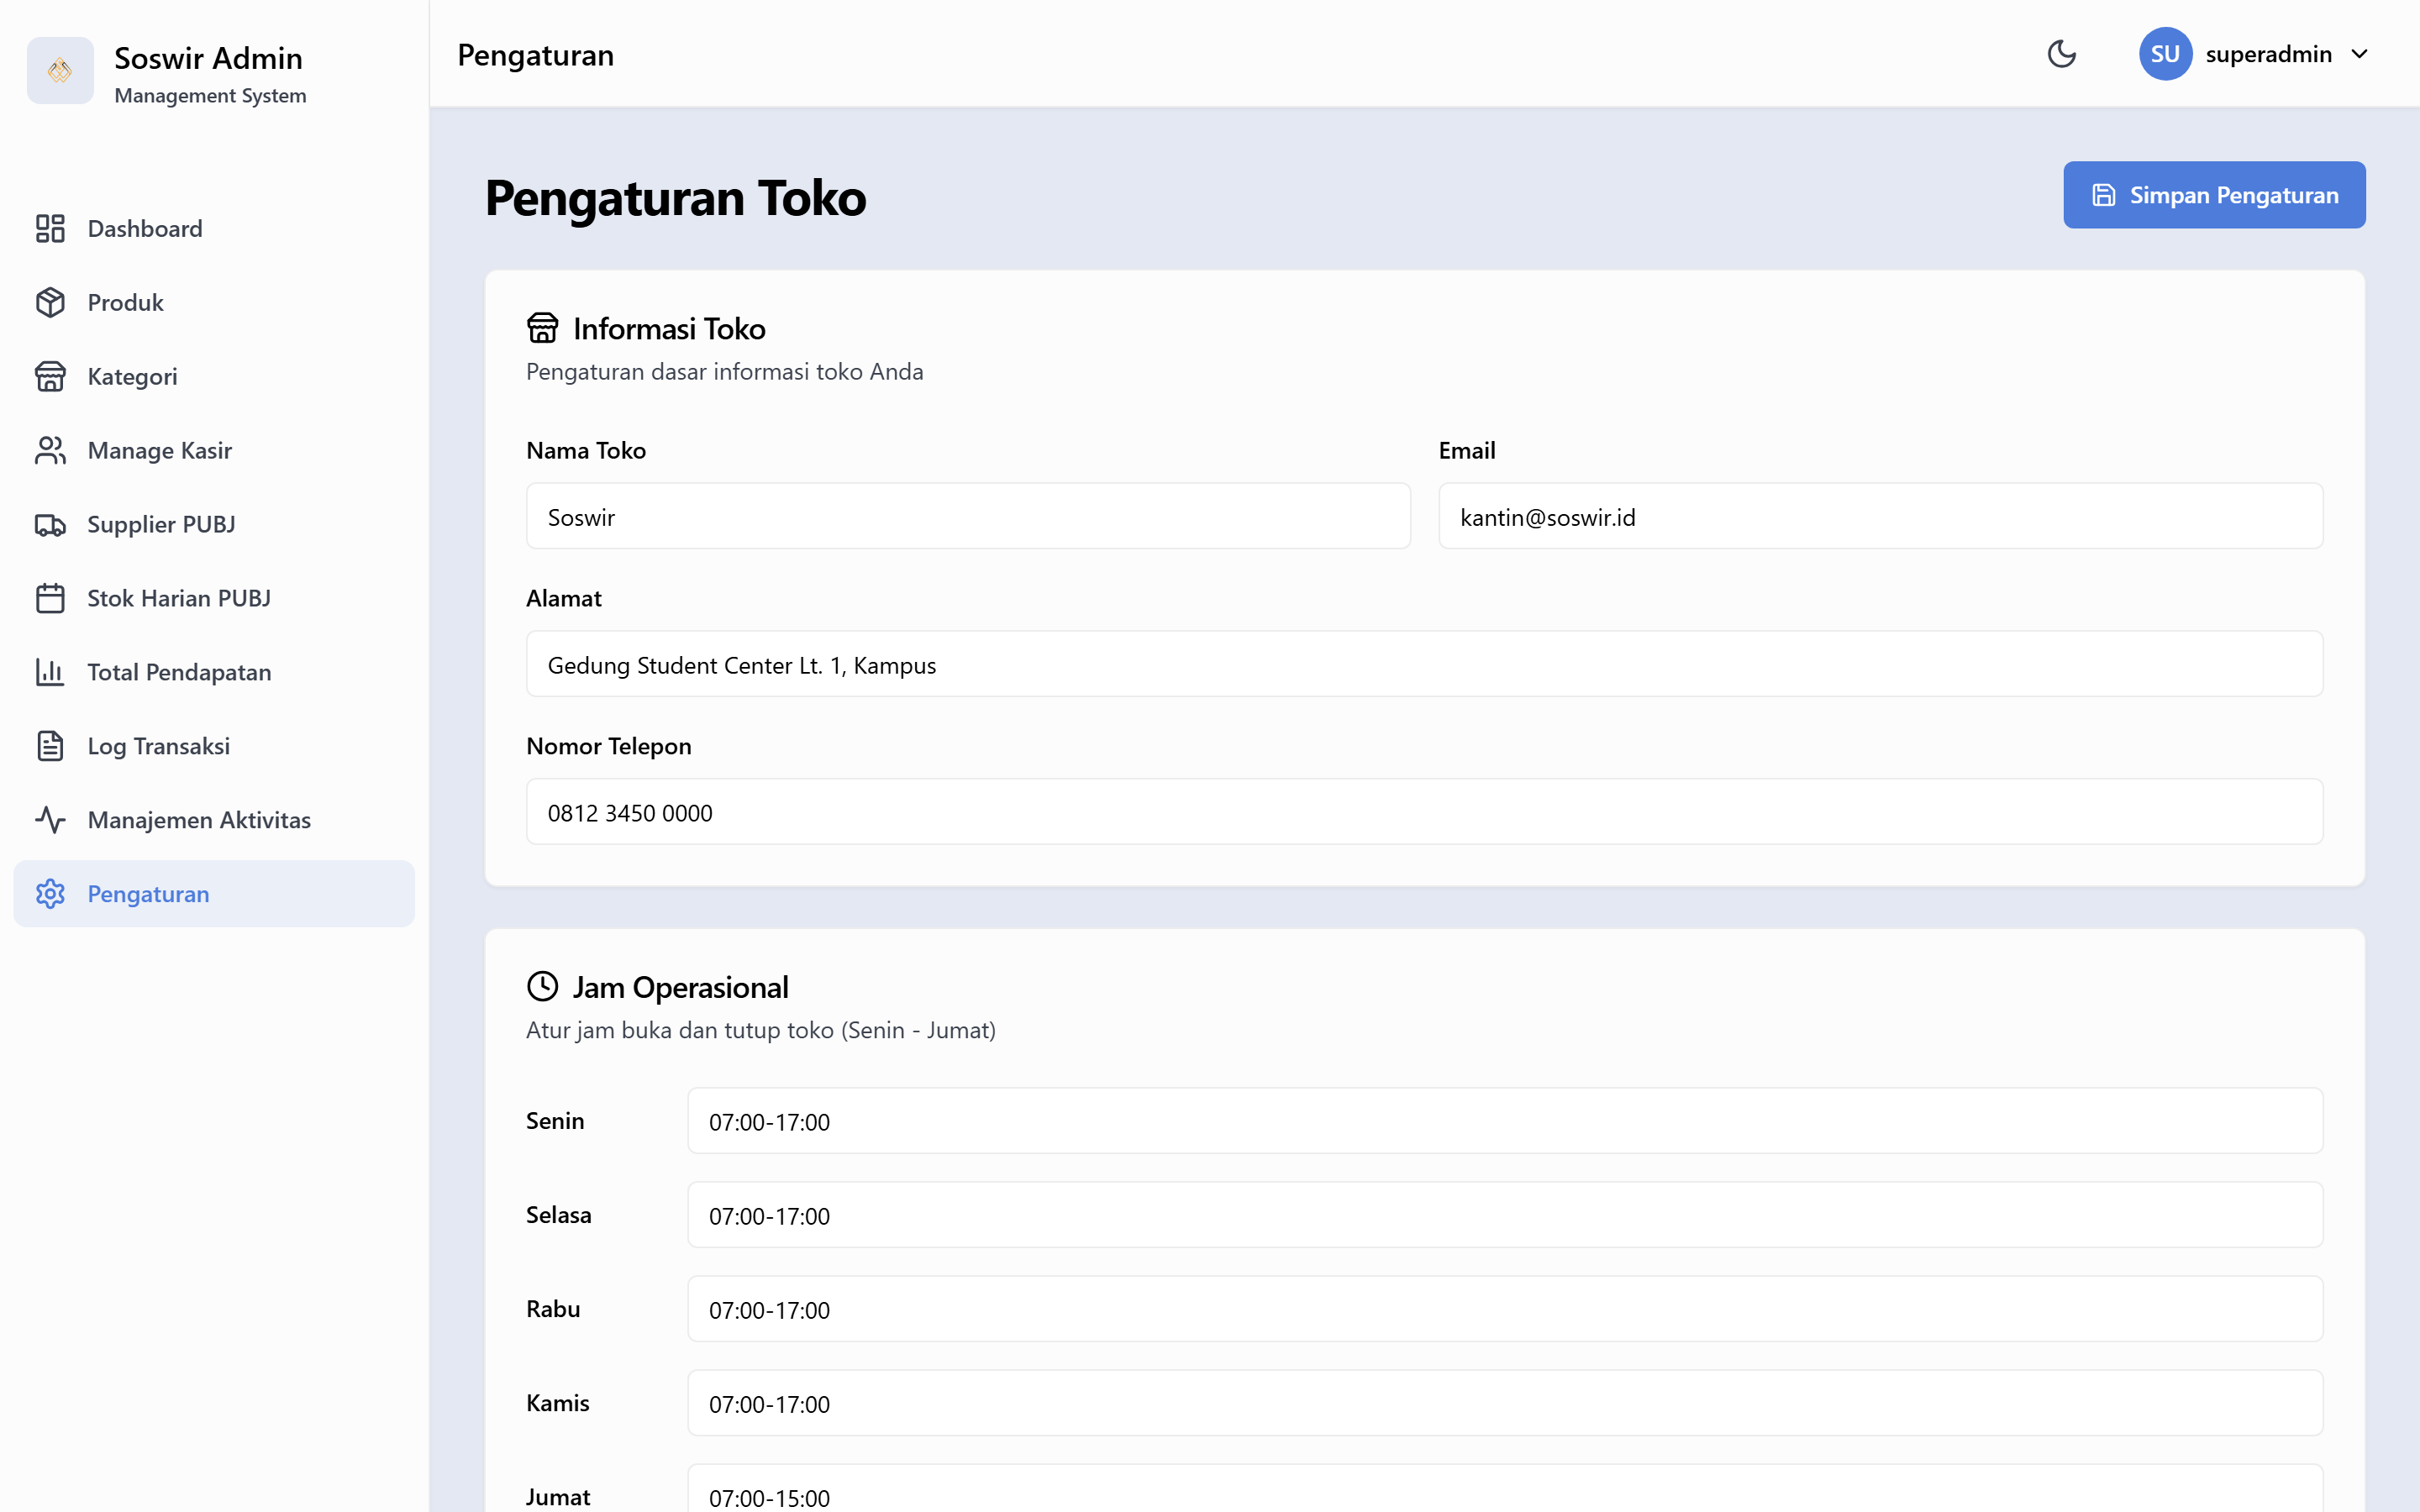
\includegraphics[width=0.99\linewidth,height=0.40\textheight,keepaspectratio,cfbox=garis 0.5pt 0pt]{img/45-pengaturan.png}
\caption{Halaman \ui{Pengaturan Toko}.}
\end{figure}

\begin{catatan}
Jam operasional di halaman ini hanya informasi toko. Jam masuk kasir diatur lewat sesi shift di \ui{Manage Kasir}.
\end{catatan}

% ---------------------------------------------------------------
\section{Tanya Jawab}

\subsection{Kasir lupa password}

Kasir tidak bisa mengatur ulang password sendiri. Superadmin membuka \ui{Manage Kasir}, memilih \ui{Edit} pada kasir tersebut, mengisi \ui{Password} dan \ui{Konfirmasi} yang baru, lalu menekan \ui{Simpan}. Kalau superadmin yang lupa password, hubungi pengelola aplikasi.

\subsection{Kasir tidak bisa masuk}

Baca pesan merah di halaman masuk.

\begin{itemize}
  \item ``Di luar jam shift Anda'': kasir mencoba masuk di luar jam sesinya. Tunggu sampai 15 menit sebelum jam mulai, atau minta superadmin memindahkan kasir ke sesi yang sesuai.
  \item ``Anda belum ditempatkan di sesi shift mana pun'': superadmin perlu memilih sesi di kolom \ui{Sesi} pada \ui{Manage Kasir}.
  \item ``Invalid credentials'': username atau password salah. Periksa huruf besar-kecil, atau minta superadmin membuatkan password baru.
\end{itemize}

\subsection{Barang titipan tidak bisa dijual}

Produk PUBJ hanya bisa dijual kalau hari ini ada entry \ui{Aktif} di \ui{Stok Harian PUBJ} dan sisanya masih ada. Setelah pukul 18:00 WIB entry ditutup otomatis, sehingga barang titipan tidak bisa dijual lagi sampai stok hari berikutnya dicatat.

\subsection{Gambar produk tidak muncul}

\begin{itemize}
  \item Pastikan file berformat JPG, PNG, atau WEBP dan ukurannya tidak lebih dari 5 MB.
  \item Buka \ui{Edit} pada produk tersebut, pilih ulang gambarnya, lalu tekan \ui{Update Produk}.
  \item Muat ulang halaman dengan tombol \ui{Refresh} atau tombol muat ulang peramban.
\end{itemize}

\subsection{Angka keuntungan toko berbeda dari total penjualan}

Itu wajar kalau ada penjualan barang titipan. Total penjualan menghitung seluruh uang yang diterima, sedangkan keuntungan toko hanya mengambil fee toko dari barang PUBJ. Selisihnya adalah hak supplier dan tampil sebagai keuntungan supplier.

\subsection{Produk tidak bisa dihapus}

Produk yang sudah pernah terjual atau punya stok harian tidak bisa dihapus permanen. Pilih \ui{Nonaktifkan} supaya produk tidak muncul lagi di kasir.

\end{document}
